% Borrador del escrito del trabajo de grado.
% Compilar con XeLaTeX:  make escrito   (o: latexmk -xelatex docs/escrito/escrito.tex)
% Cada capítulo está en capitulos/; las figuras se toman de figuras/limpias/, figuras/ y presentacion/img/.
\documentclass[11pt,a4paper,oneside]{report}

\usepackage[a4paper,margin=2.5cm]{geometry}
\usepackage{fontspec}
\usepackage[spanish,es-noshorthands,es-tabla]{babel}
\usepackage{amsmath,amssymb,amsthm,mathtools}
\usepackage{graphicx}
\usepackage{booktabs,tabularx,longtable,multirow}
\usepackage{xcolor}
\usepackage{enumitem}
\usepackage{microtype}
\usepackage{caption}
\usepackage{subcaption}
\usepackage{csquotes}
\usepackage[section]{placeins}
\usepackage[round,authoryear]{natbib}
\usepackage[algoruled,linesnumbered,spanish,onelanguage]{algorithm2e}
\usepackage[hidelinks]{hyperref}

% Primero las versiones sin títulos ni notas (los textos van en las leyendas del documento).
\graphicspath{{figuras/limpias/}{../../presentacion/img/}{figuras/}}
% Flotantes: más espacio en página para figuras, para que no se acumulen al final de un capítulo.
\renewcommand{\topfraction}{0.85}
\renewcommand{\bottomfraction}{0.6}
\renewcommand{\textfraction}{0.1}
\renewcommand{\floatpagefraction}{0.75}
\setcounter{topnumber}{3}
\setcounter{bottomnumber}{2}
\setcounter{totalnumber}{5}
\setlist{itemsep=2pt,topsep=4pt}
\captionsetup{font=small,labelfont=bf}
\setlength{\parskip}{0.35em}

% Notación musical y marcas del borrador
\newcommand{\fl}{\ensuremath{\flat}}
\newcommand{\sh}{\ensuremath{\sharp}}
\newcommand{\cuarto}{\ensuremath{\tfrac14}}
\newcommand{\edo}[1]{#1\nobreakdash-EDO}
\newcommand{\pv}[1][]{\textcolor{red!70!black}{\,[por verificar#1]}}
\newcommand{\pendiente}[1]{\textcolor{orange!80!black}{[Pendiente: #1]}}
\DeclareMathOperator{\mcd}{mcd}
\DeclareMathOperator{\round}{round}

\theoremstyle{definition}
\newtheorem{definicion}{Definición}[chapter]
\newtheorem{proposicion}[definicion]{Proposición}
\newtheorem{ejemplo}[definicion]{Ejemplo}

\begin{document}

\begin{titlepage}
  \centering
  {\large Universidad Nacional de Colombia, sede Bogotá\\
  Facultad de Ciencias · Departamento de Matemáticas\par}
  \vspace{3cm}
  {\LARGE\bfseries Microtonalidad en 24-EDO, bucles y ciclos armónicos\\[0.3em]
  en Angine de Poitrine:\\[0.3em] un análisis computacional del \emph{Vol.~II}\par}
  \vspace{1.5cm}
  {\large Trabajo de grado\par}
  \vspace{2cm}
  {\large Santiago Forero Rosales\par}
  \vspace{0.8cm}
  {\normalsize Director: Jorge Eliecer Camargo Mendoza\par}
  \vfill
  {\normalsize Bogotá, 2026\par}
  \vspace{0.5cm}
  {\small\textcolor{red!70!black}{Primer borrador. Las marcas en rojo («por verificar») y en naranja («Pendiente») señalan lo que falta comprobar o completar.}\par}
\end{titlepage}

\pagenumbering{roman}
\chapter*{Resumen}
\addcontentsline{toc}{chapter}{Resumen}

Angine de Poitrine es un dúo de Saguenay (Quebec) que toca con guitarra y bajo de trastes de cuarto de tono, construye
sus canciones con un looper y usa compases poco comunes. Este trabajo pregunta si su música encaja en un estilo
existente o si es una propuesta nueva, y responde la pregunta midiendo desde el audio. Para ello se construyó una
herramienta abierta que transcribe en 24-EDO (veinticuatro divisiones iguales de la octava): separa la guitarra y el
bajo, estima la altura con una saliencia armónica en una rejilla de 25 cents, usa la repetición del looper para
estabilizar la transcripción, segmenta la canción en compases y asigna a cada compás un acorde con las calidades de
Piston extendidas a 24-EDO, sus funciones (Riemann) y sus ejes (Lendvai). La salida principal es el \emph{tabroll}, un
piano roll de 24 filas por octava con los acordes debajo.

La herramienta se evaluó contra partituras corregidas de oído, con arbitrajes a ciegas y una canción reservada como
prueba ciega. La fundamental del acorde acierta en promedio el 85\,\% en los compases confiables, mientras que la
melodía acierta el 49\,\%; la diferencia se explica por la forma en que se decide la armonía (peso del bajo, suma
sobre las vueltas del loop, independencia de la octava y resolución por compás). Con esa base, cada canción del álbum
\emph{Vol.~II} se resumió en cuatro bloques de rasgos (armonía, escala, cuartos de tono y metro) y se comparó con seis
corpus de estilos mediante la distancia de Jensen-Shannon y un percentil de tipicidad, después de aplicar a los corpus
el error de medición de la propia herramienta, estimado con canciones de control.

Los resultados indican que la banda es un híbrido con un elemento propio. En armonía, ninguna canción es típica de
ningún corpus (máximo 17.7 sobre 50) y el 37.5\,\% de los casos queda sin vecino, frente al 5.2\,\% en piezas reales de
rock. En melodía, dos grados en cuarto de tono concentran entre el 48 y el 82\,\% de los cuartos de tono de cada
canción: son grados fijos de la escala, no adornos, y forman dos familias (frigia y dórica), de las cuales la dórica no
aparece en ningún corpus medido. En metro, los ciclos del looper muestran periodos de 20 y 28 corcheas, compatibles con
compases de 5 y de 7 tiempos. La conclusión es que la música de la banda no corresponde a un estilo existente, sino a
una recombinación de lenguajes conocidos con un rasgo nuevo: los cuartos de tono como grados fijos de la escala.

\medskip
\noindent\textbf{Palabras clave:} microtonalidad, 24-EDO, transcripción automática, recuperación de información musical,
armonía funcional, corpus de estilos, divergencia de Jensen-Shannon, Angine de Poitrine.

\chapter*{Abstract}
\addcontentsline{toc}{chapter}{Abstract}

\pendiente{traducir el resumen al inglés cuando el texto en español quede estable.}


\tableofcontents
\listoffigures
\listoftables

\cleardoublepage
\pagenumbering{arabic}
\chapter{Introducción}\label{cap:introduccion}

\section{Motivación}

En diciembre de 2025 KEXP grabó a Angine de Poitrine en el festival Trans Musicales de Rennes; el video, publicado en
febrero de 2026, pasaba de 7.5 millones de reproducciones en YouTube a fines de marzo \citep{kexp2026}. Lo que llama la atención al escucharla es una combinación poco frecuente: una guitarra y
un bajo con trastes de cuarto de tono, canciones que se construyen capa por capa con un looper y compases que no son los
habituales del rock. Esa combinación plantea la pregunta que
guía este trabajo:

\begin{quote}
\itshape ¿La música de Angine de Poitrine encaja en un estilo existente o es una propuesta nueva?
\end{quote}

Responderla de oído es difícil, porque la banda mezcla rasgos de tradiciones muy distintas. Responderla por computador
también lo es, porque las herramientas estándar de análisis musical piensan en doce notas por octava: \texttt{music21}
comprime toda altura a doce clases y los transcriptores automáticos redondean cada cuarto de tono al semitono más
cercano. Para esta música, medir en doce notas es borrar justamente lo que la hace distinta. Por eso el trabajo empieza
por construir una herramienta que mida en veinticuatro.

\section{Qué es un análisis computacional}

Un análisis computacional asigna a una pieza una macroestructura (resultados visuales, datos o patrones) a partir de un
programa que lee la información contenida en su registro. La obra musical es un objeto abstracto, una actividad, pero sus
registros existen en contextos concretos: una grabación, una partitura, un archivo. El programa permite reconstruir de
manera empírica, y repetible, el fundamento técnico de esos registros.

La entrada de un análisis así es siempre una representación, y ninguna representación es única. Un mismo audio en WAV y
en FLAC no contiene el mismo flujo de datos; un MP3 de baja calidad pierde información que un formato sin compresión
conserva; MusicXML y MIDI hacen explícitos los compases y las alturas, pero solo los que alguien decidió escribir. La
representación de una pieza queda indeterminada de tres maneras: por cómo se proyectan los datos, por qué datos se
seleccionan y por la información que se introduce desde fuera (o la incertidumbre sobre si existe). Por eso el diagrama
de análisis necesita revisión constante para reflejar las variaciones entre entradas, incluso cuando corresponden a la
misma pieza.

En ese sentido, el análisis computacional busca cómo una pieza establece sus propios principios explicativos. Para que sea
útil, su resultado debe tener una estructura temporal, contener menos información que la pieza que resume y cumplir un
protocolo explícito que limite los sesgos de quien analiza. En este trabajo, ese protocolo es concreto: la herramienta
nunca lee la partitura, la referencia se corrige de oído y a ciegas, el azar queda fijo y el error de la propia
herramienta se mide y se aplica a los corpus con que se compara.

\section{La banda}

Angine de Poitrine es un dúo formado en 2019 en Saguenay, Quebec. Sus integrantes usan los seudónimos Khn y Klek de
Poitrine: Khn toca la guitarra y el bajo microtonales y Klek, la batería \citep{weller2026,dunlevie2026}. Su música es rock instrumental del tipo que se
suele llamar \emph{math rock}: riffs en bucle que se superponen, en compases poco comunes. Su afinación es 24-EDO, es
decir, veinticuatro notas igualmente espaciadas por octava, el doble que la guitarra común; cada traste nuevo del
instrumento agrega un cuarto de tono (50 cents). El objeto de estudio es su álbum \emph{Vol.~II} (3 de abril de 2026)
completo, en el orden de sus pistas: Fabienk, Mata Zyklek, Sarniezz, Utzp, Yor Zarad y Angor.

El nombre de la banda es el término francés para la angina de pecho, el dolor torácico causado por la falta de
oxígeno en el corazón.

\section{Influencias declaradas y comparaciones}\label{sec:influencias}

Las influencias que se ponen a prueba provienen de tres fuentes distintas, y conviene separarlas desde el principio:

\begin{itemize}
  \item \textbf{Lo que dice la banda.} En la entrevista de \emph{Noize Magazine}, Khn cuenta que al principio tiraban más
  al rock turco y que siguen escuchando rock turco y música de Medio Oriente; que usa los cuartos de tono con un fraseo
  «más cubista, más a lo Zappa»; y que la armonía de casi todos sus temas se compara con el \emph{Überjam} de John
  Scofield o con «So What» de Miles Davis. Klek dice que su banda favorita es Gentle Giant
  \citep{noize}. En el podcast \emph{Aucard de Tours}, Khn describe una música construida sobre loops, con la
  repetición del techno en la estructura y no en el timbre, y con la idea de que la gente baile «en 5 y en 7»
  \citep{aucard2026}.
  \item \textbf{Lo que dicen los analistas.} Mathémusique (Paul Lascabettes) pone como precedente a King Gizzard and the
  Lizard Wizard, que en 2017 pasó de doce a veinticuatro notas en \emph{Flying Microtonal Banana}; la banda no lo cita
  \citep{mathemusique2026}. David Bennett afirma que en uno de sus temas los cuartos de tono se usan como en el maqam
  hijaz, «casi» un frigio dominante \citep{bennett2026}.
  \item \textbf{Una comparación propia.} Primus se eligió al estudiar su armonía. Ninguna fuente pública consultada lo
  cita como influencia de la banda; en este trabajo cumple el papel de control, porque es rock sin cuartos de tono.
\end{itemize}

Cada influencia apunta a una dimensión que se puede medir: el rock turco y el maqam a la escala; Zappa y Gentle Giant a
la melodía y la métrica; Scofield y Miles Davis a la armonía; el techno y los loops a la forma en ciclos; y la
declaración «en 5 y en 7» al metro. Así la pregunta general se descompone en preguntas que se contrastan dimensión por
dimensión.

\section{Hipótesis}

\begin{quote}
La banda puede ser típica en cada dimensión (armonía, melodía y ritmo) de un estilo distinto, pero atípica en la
combinación: una recombinación nueva de lenguajes existentes.
\end{quote}

La hipótesis nula correspondiente es que, una vez descontado el error de medición de la herramienta, el álbum no se
distingue del rock. La calibración del método con piezas reales de rock (capítulo~\ref{cap:resultados}) es lo que
permite rechazarla o no.

\section{Objetivos}

\paragraph{Objetivo general.} Decidir, a partir del audio, si la música de Angine de Poitrine cabe en un estilo
existente o constituye una propuesta nueva.

\paragraph{Objetivos específicos.}
\begin{enumerate}
  \item Transcribir desde el audio la melodía, el bajo, los compases y los acordes en 24-EDO.
  \item Medir los ciclos del looper y el uso de los cuartos de tono, con un control que estime el error de la propia
  herramienta.
  \item Evaluar la transcripción contra referencias corregidas de oído, con un protocolo a ciegas.
  \item Comparar cada dimensión con corpus de estilos y con repertorios de referencia, y combinar las comparaciones en
  un veredicto calibrado.
\end{enumerate}

\section{Aportes}

\begin{enumerate}
  \item \textbf{Una herramienta:} transcripción y análisis armónico abiertos en 24-EDO, desde el audio polifónico, guiados
  por la repetición del looper. Su salida es el tabroll.
  \item \textbf{Un método:} comparación con corpus reales de estilos por bloques de rasgos, con el error de la
  herramienta aplicado a los corpus y calibrada para no exagerar la novedad.
  \item \textbf{Un resultado:} una respuesta medida a la pregunta de si la banda es un estilo existente o una propuesta
  nueva.
\end{enumerate}

\section{Organización del documento}

El capítulo~\ref{cap:marco} presenta el marco matemático y musical: la medida de la altura en 24-EDO, las herramientas de
procesamiento de señales, la teoría armónica que se extiende y las medidas estadísticas de comparación. El
capítulo~\ref{cap:estado} resume el estado del arte y el vacío que cubre el trabajo. El capítulo~\ref{cap:datos}
describe los datos: el álbum, las referencias, los controles y los corpus. El capítulo~\ref{cap:metodologia} cuenta
cómo evolucionó el método y describe el algoritmo final, su evaluación y la comparación con estilos, y el
capítulo~\ref{cap:herramienta}, cómo está construida la herramienta y qué garantiza su reproducibilidad. El
capítulo~\ref{cap:resultados} presenta los resultados, el capítulo~\ref{cap:discusion} discute sus límites y el
capítulo~\ref{cap:conclusiones} cierra con las conclusiones y el trabajo futuro.

\chapter{Marco teórico}\label{cap:marco}

Este capítulo reúne las herramientas que usa el trabajo. La sección~\ref{sec:altura} define cómo se mide la altura en
24-EDO y la estructura algebraica de sus clases. La sección~\ref{sec:senal} resume el procesamiento de señales que lleva
del audio a las alturas. La sección~\ref{sec:armonia-teoria} presenta la teoría armónica que se extiende a 24-EDO, y la
sección~\ref{sec:estadistica}, las medidas con que se comparan canciones y estilos.

\section{La altura en 24-EDO}\label{sec:altura}

\subsection{Escala logarítmica y cents}

La percepción de la altura es aproximadamente logarítmica en la frecuencia: subir una octava es multiplicar la frecuencia
por dos. Para medir distancias de manera lineal se usa el \emph{cent}.

\begin{definicion}[Cents]
La distancia en cents entre una frecuencia $f$ y una frecuencia de referencia $f_0$ es
\[
  c(f, f_0) = 1200 \log_2\!\left(\frac{f}{f_0}\right).
\]
Una octava mide 1200 cents y un semitono del temperamento de doce notas, 100.
\end{definicion}

\begin{definicion}[$q$-EDO]
En el sistema $q$-EDO (\emph{equal divisions of the octave}) la octava se divide en $q$ pasos iguales. Cada paso mide
$1200/q$ cents y corresponde a la razón de frecuencias
\[
  \rho_q = 2^{1/q}, \qquad f_j = f_{\mathrm{ref}}\, 2^{j/q}.
\]
\end{definicion}

Para $q = 12$ se obtiene el temperamento igual usual. Para $q = 24$ cada paso mide 50 cents, un cuarto de tono, y la razón
entre pasos consecutivos es $\alpha = 2^{1/24} \approx 1.0293$: cada traste del instrumento de la banda sube la frecuencia
cerca de un 2.93\,\%. Esta rejilla es la que forma las filas del tabroll.

\subsection{MIDI fraccionario y clases de altura}

El estándar MIDI numera las teclas del piano con enteros y asigna el número 69 al La de 440~Hz \citep{midi1996}. Su
extensión continua permite números fraccionarios:
\[
  M(f) = 69 + 12 \log_2\!\left(\frac{f}{440}\right).
\]
Así, el Mi de la nota 52 subido 50 cents queda en $M = 52.5$: un cuarto de tono sobre Mi, que un sistema de doce notas
redondearía a Mi o a Fa. La clase de altura en 24-EDO se obtiene redondeando al medio semitono y reduciendo módulo la
octava:
\[
  \operatorname{pc}_{24}(M) = \round(2M) \bmod 24 \in \mathbb{Z}_{24}.
\]
Una altura cae en una casilla de 24-EDO si está a menos de 25 cents de su centro. Las clases pares son los doce grados
regulares (Do, Do\sh, Re, \dots) y las impares, los doce grados en cuarto de tono, que se escriben con «+»: Do+, Re+,
etc. Los grados se cuentan desde la tónica de la canción; por ejemplo, \fl2+ es el segundo grado rebajado un semitono y
subido un cuarto de tono.

Contar los grados desde la tónica $t$ equivale a aplicar la transposición $T_{-t}$, con $T_k(y) = y + k$ en
$\mathbb{Z}_{24}$, así que los perfiles y los grados de este trabajo son los mismos en cualquier tonalidad. Las
transposiciones y las inversiones $I_n(y) = n - y$ forman juntas el grupo diédrico $D_{24}$, de 48 elementos: las simetrías
de un polígono de 24 lados \citep{crans2009,flynn2025}. La herramienta usa solo las transposiciones, a propósito: una
inversión convierte una tríada mayor en una menor ($I_0$ lleva Do mayor a fa menor), y esa diferencia es una de las que
se quieren medir.

\subsection{Los dos campos de quintas}\label{sec:campos}

En 24-EDO la quinta justa temperada mide 700 cents, es decir, 14 pasos de cuarto de tono. El ciclo de quintas es la
órbita de una clase bajo la suma reiterada de 14 en $\mathbb{Z}_{24}$.

\begin{proposicion}\label{prop:campos}
El subgrupo de $\mathbb{Z}_{24}$ generado por $14$ es $\langle 14 \rangle = \langle 2 \rangle = \{0, 2, 4, \dots, 22\}$,
de orden 12. En consecuencia, el ciclo de quintas de 24-EDO se parte en dos órbitas disjuntas de doce clases: los grados
regulares (clases pares) y los grados en cuarto de tono (clases impares).
\end{proposicion}

\begin{proof}
En un grupo cíclico $\mathbb{Z}_n$, el subgrupo generado por $a$ es el generado por $\mcd(a, n)$ y tiene orden
$n / \mcd(a, n)$. Como $\mcd(14, 24) = 2$, se tiene $\langle 14 \rangle = \langle 2 \rangle$, de orden $24/2 = 12$. Sus
dos clases laterales, $\langle 2 \rangle$ y $1 + \langle 2 \rangle$, son las clases pares e impares, y la suma de 14
conserva la paridad.
\end{proof}

Cada órbita se llama un \emph{campo}. Alois Hába armonizaba dentro de un solo campo y pasaba de uno al otro por la
melodía, lo que se ha llamado «desplazamiento de campos» \citep{little2019}. En su tratado, Hába describe la gama de
cuartos de tono como dos mitades, los doce grados convencionales y los doce en cuarto de tono, y para pasar de una a otra
recomienda movimiento contrario en las voces extremas \citep[cap.~II]{haba1927}; \citet[cap.~3]{skinner2006} encuentra en
su \emph{Suite für vier Posaunen}, op.~72, acordes puramente convencionales que alternan con acordes puramente en cuarto
de tono, aunque la regla del movimiento contrario no siempre se cumple. El manual de Wyschnegradsky deja ver por qué
funciona esa regla: dos escalas de cuartos de tono en movimiento contrario que parten del unísono dan, paso a paso, todos
los intervalos tradicionales \citep[§11, p.~6]{wyschnegradsky2017}. Cada voz cambia de campo en cada paso, pero las dos lo
hacen a la vez, así que nunca quedan en campos distintos. En las figuras del círculo de 24-EDO
(capítulo~\ref{cap:resultados}) el anillo exterior es el campo regular y el interior, el de cuarto de tono; cada grado
«+» queda junto a su vecino regular.

La misma imagen aparece en Ivan Wyschnegradsky. En su \emph{Manuel d'harmonie à quarts de ton} (1932) describe los doce
grados nuevos como la relación entre dos escalas cromáticas, una transportada un cuarto de tono, que se parecen a dos
peines cuyos dientes encajan \citep[§3, p.~1]{wyschnegradsky2017}. En el mismo manual observa que el ciclo de terceras
neutras recorre las 24 notas y se parte en dos ciclos de quintas, separados por una tercera neutra
\citep[§10, p.~5]{wyschnegradsky2017}. Es la proposición~\ref{prop:campos} vista desde la tercera neutra: como
$\mcd(7, 24) = 1$, sumar 7 recorre todo $\mathbb{Z}_{24}$, y sumar 7 dos veces es sumar 14, la quinta, que no sale del
campo. Charles Ives la llevó al instrumento en sus \emph{Three Quarter-Tone Pieces}
(1923--1924), para dos pianos afinados a un cuarto de tono de distancia \citep{ives1968}: un piano toca solo el campo
regular y el otro, solo el de cuarto de tono \citep{flynn2025}.

\begin{proposicion}\label{prop:z12}
La aplicación $\iota : \mathbb{Z}_{12} \to \mathbb{Z}_{24}$, $\iota(r) = 2r$, es un monomorfismo de grupos cuya imagen es
el campo regular $\langle 2 \rangle$. En consecuencia, todo análisis en doce notas se reproduce dentro de 24-EDO, y el
campo de cuarto de tono es la clase lateral $1 + \iota(\mathbb{Z}_{12})$, que ningún análisis en doce notas puede ver.
\end{proposicion}

\begin{proof}
$\iota(r + s) = 2(r + s) = \iota(r) + \iota(s)$ módulo 24, y $\iota(r) = 0$ en $\mathbb{Z}_{24}$ implica $24 \mid 2r$, es
decir, $12 \mid r$, de modo que $r = 0$ en $\mathbb{Z}_{12}$. La imagen tiene 12 elementos, todos pares, así que es
$\langle 2 \rangle$.
\end{proof}

\subsection{Razones justas y su aproximación en 24-EDO}

Los intervalos «naturales» de la serie armónica corresponden a razones de enteros pequeños: la octava $2/1$, la quinta
$3/2$, la tercera mayor $5/4$. Un sistema $q$-EDO aproxima cada razón $r$ por el paso más cercano.

\begin{proposicion}
Sea $c(r) = 1200 \log_2 r$ el tamaño en cents de la razón $r$. Su mejor aproximación en $q$-EDO,
$\hat c(r) = \tfrac{1200}{q} \round\!\bigl(\tfrac{q}{1200} c(r)\bigr)$, cumple $|c(r) - \hat c(r)| \le 600/q$. Además,
el error en 24-EDO nunca es mayor que el error en 12-EDO.
\end{proposicion}

\begin{proof}
La primera afirmación es la cota del redondeo al múltiplo más cercano de $1200/q$. Para la segunda, la rejilla de 12-EDO
está contenida en la de 24-EDO (proposición~\ref{prop:z12}), así que el punto más cercano en la rejilla fina está al
menos tan cerca como el más cercano en la gruesa.
\end{proof}

La tabla~\ref{tab:razones} muestra por qué 24-EDO no es solo «12-EDO con más notas»: aproxima intervalos de la serie
armónica que 12-EDO no tiene, como la tercera neutra $11/9$ y la segunda neutra $12/11$, presentes en el maqam árabe. Los nombres de los
intervalos nuevos son los de \citet[§6, pp.~2--3]{wyschnegradsky2017}: segunda, tercera, sexta y séptima neutras (3, 7,
17 y 21 cuartos de tono), a medio camino entre la menor y la mayor.

\begin{table}[ht]
  \centering
  \caption{Algunas razones justas y su aproximación en 12-EDO y en 24-EDO (en cents).}\label{tab:razones}
  \begin{tabular}{@{}llrrr@{}}
    \toprule
    Intervalo & Razón & Justo & 12-EDO (error) & 24-EDO (error) \\
    \midrule
    Quinta justa & $3/2$ & 702.0 & 700 ($-2.0$) & 700 ($-2.0$) \\
    Tercera mayor & $5/4$ & 386.3 & 400 ($+13.7$) & 400 ($+13.7$) \\
    Tercera menor & $6/5$ & 315.6 & 300 ($-15.6$) & 300 ($-15.6$) \\
    Tercera neutra & $11/9$ & 347.4 & 300 o 400 ($\pm 50$) & 350 ($+2.6$) \\
    Segunda neutra & $12/11$ & 150.6 & 100 o 200 ($\pm 50$) & 150 ($-0.6$) \\
    Cuarta del 11.º armónico & $11/8$ & 551.3 & 500 o 600 ($\pm 50$) & 550 ($-1.3$) \\
    \bottomrule
  \end{tabular}
\end{table}

\section{Microtonalidad, modos y looper}\label{sec:contexto-musical}

\subsection{Modos}

Un \emph{modo} es una escala de siete grados con un centro. Los modos que aparecen en este trabajo se distinguen por
los grados 2, 3, 6 y 7, medidos en semitonos sobre la tónica:

\begin{itemize}
  \item \textbf{Dórico:} 1, 2, \fl3, 4, 5, 6, \fl7. Es un menor con la sexta mayor; «So What» de Miles Davis, que la banda
  menciona, está en dórico.
  \item \textbf{Frigio:} 1, \fl2, \fl3, 4, 5, \fl6, \fl7. Es un menor con la segunda rebajada, de sonido «oriental» o
  «flamenco».
  \item \textbf{Frigio dominante:} 1, \fl2, 3, 4, 5, \fl6, \fl7. Es el frigio con la tercera mayor; entre \fl2 y 3 queda
  una segunda aumentada. Es la escala más cercana, en doce notas, al maqam hijaz.
  \item \textbf{Mixolidio:} 1, 2, 3, 4, 5, 6, \fl7. Es un mayor con la séptima rebajada, frecuente en el rock.
\end{itemize}

En 24-EDO cada uno de esos grados puede aparecer además en su versión neutra, un cuarto de tono por encima de la
rebajada, con el nombre que \citet[§6]{wyschnegradsky2017} da a esos intervalos: \fl2+, \fl3+, \fl6+ y \fl7+ son la
segunda, la tercera, la sexta y la séptima neutras. La herramienta no fuerza un nombre de doce notas: describe el modo por la versión de los grados 2, 3, 6 y 7 que
más suena (por ejemplo «\fl2+, 3, \fl6+, \fl7»).

\subsection{La microtonalidad en otras tradiciones}

\paragraph{Maqam árabe.} La teoría árabe del siglo XX describe sus escalas sobre una rejilla de 24 cuartos de tono \citep{touma1996},
aunque la afinación real de cada intervalo varía según el maqam y la región. Varios maqamat usan segundas y terceras
neutras (por ejemplo rast y bayati). Hijaz, el que menciona David Bennett, se caracteriza por la segunda aumentada entre
el segundo y el tercer grado, y en doce notas se parece al frigio dominante \citep{touma1996}.

\paragraph{Makam turco.} La teoría de Arel, Ezgi y Uzdilek divide el tono en nueve comas de Holder (la octava en 53
partes), lo que da intervalos que no caen en 24-EDO. Por eso SymbTr guarda las alturas en comas \citep{karaosmanoglu2012}
y los estudios de altura del makam usan histogramas finos \citep{bozkurt2008,gedik2010}.

\paragraph{Radif persa.} El radif es el repertorio clásico de la música persa, organizado en siete \emph{dastgah} y cinco
\emph{avaz} \citep{farhat1990}. La notación moderna usa dos alteraciones microtonales: el \emph{koron}, que baja una nota
aproximadamente un cuarto de tono, y el \emph{sori}, que la sube \citep{kanani2025}.

\paragraph{Alois Hába.} El compositor checo Alois Hába (1893--1973) escribió obras en cuartos, quintos y sextos de
tono, y en 1927 publicó la \emph{Neue Harmonielehre}, una teoría de la armonía para los sistemas de tercios, cuartos,
sextos y doceavos de tono \citep{haba1927,choroscian2018}. Su música en cuartos de tono se ha estudiado en los cuartetos
de cuerda \citep{choroscian2018}, en las obras para violín solo \citep{jin2015} y en la suite para cuatro trombones
\citep{skinner2006}; desde 1924 enseñó cuartos de tono en el Conservatorio de Praga y trabajó con la casa Förster en
pianos y armonios de cuarto y sexto de tono \citep{spurny2021}. Su idea de armonizar dentro de un campo y desplazarse
entre campos por la melodía es la que se pone a prueba en la sección~\ref{sec:res-haba}.

\paragraph{King Gizzard and the Lizard Wizard.} En \emph{Flying Microtonal Banana} (2017) la banda australiana usó
guitarras y bajos con trastes de cuarto de tono, es decir, el mismo 24-EDO que Angine de Poitrine; la nota de
lanzamiento del álbum termina con «24-TET EVERYBODY» \citep{kinggizzard2017}. Es el precedente más
cercano en el rock y por eso entra en la comparación (sección~\ref{sec:repertorios}).

\subsection{El looper}

Un looper es un dispositivo que graba una frase y la reproduce en bucle mientras el músico toca encima; cada nueva capa
se suma a las anteriores (\emph{overdub}). Una canción construida así tiene tres propiedades que el método aprovecha y
que, a la vez, lo dificultan:
\begin{enumerate}
  \item \textbf{Periodicidad:} dentro de una sección, el audio se repite con un periodo fijo, el largo del bucle. Esto
  permite promediar entre vueltas (sección~\ref{sec:met-consenso}).
  \item \textbf{Tempo constante:} el bucle no cambia de velocidad, de modo que la alineación con la partitura puede
  ajustarse a una recta por sección (sección~\ref{sec:evaluacion}).
  \item \textbf{Capas del mismo instrumento:} varias guitarras grabadas por la misma persona, con el mismo timbre, suenan a
  la vez. Ningún separador de fuentes las distingue, y ese es el cuello de botella de la melodía
  (sección~\ref{sec:res-separacion}).
\end{enumerate}

\section{Del audio a las alturas}\label{sec:senal}

\subsection{Transformada de Fourier de tiempo corto}

Un audio digital es una sucesión de amplitudes $x[n] = x(n/f_s)$, con $f_s$ la frecuencia de muestreo. Para saber qué
frecuencias suenan en cada instante, la señal se divide en ventanas y a cada una se le aplica la transformada discreta
de Fourier:
\begin{align*}
  X(m, k) &= \sum_{n=0}^{N-1} x[n + mH]\, w[n]\, e^{-2\pi i k n / N}, &
  f_k &= \frac{k f_s}{N},
\end{align*}
donde $w$ es la ventana, $N$ su tamaño y $H$ el salto entre ventanas. El espectrograma $S(m,k) = |X(m,k)|^2$ muestra
cómo cambia el contenido frecuencial en el tiempo. Una ventana larga mejora la resolución en frecuencia y empeora la
temporal; en este trabajo la ventana del análisis de altura es de 4096 muestras (186~ms a 22\,050~Hz), lo que hace que
las notas se detecten ligeramente antes de su ataque real (sección~\ref{sec:circulo-vivo}).

\subsection{Saliencia armónica}

Una nota de guitarra no es una sola frecuencia: tiene una fundamental $f$ y armónicos en $2f, 3f, \dots$. La
\emph{saliencia armónica} estima, para cada altura candidata $p$ y cada instante $t$, cuánta evidencia hay de que esa
altura suene, sumando la energía de sus armónicos con pesos decrecientes:
\[
  \Sigma(t, p) = \sum_{h=1}^{H} \beta^{\,h-1}\, \bigl| X\bigl(t,\, h f_p\bigr) \bigr|,
\]
con $H = 10$ armónicos, $\beta = 0.82$ y una altura candidata cada 25 cents, la mitad de un paso de 24-EDO. A diferencia
de un estimador de una sola voz, la saliencia mira todas las alturas a la vez, lo que permite seguir la melodía en una
textura polifónica \citep{salamon2012}.

\subsection{pYIN y el seguimiento de la altura}

pYIN \citep{mauch2014} estima la frecuencia fundamental de una sola voz buscando cada cuánto se repite la onda, a partir
del método YIN \citep{decheveigne2002}, y elige entre las lecturas posibles el camino más probable con un modelo oculto
de Markov. Funciona bien en una línea monofónica, pero entrega una sola altura por instante.

\subsection{El algoritmo de Viterbi}

El algoritmo de Viterbi \citep{viterbi1967} encuentra, en una sucesión de estados con puntajes locales y costos de
transición, la sucesión de puntaje máximo. Sea $\{1, \dots, N\}$ el conjunto de estados (las alturas candidatas), $e_t(j)$
el puntaje de estar en el estado $j$ en el instante $t$ y $c(i, j) \ge 0$ el costo de pasar de $i$ a $j$. El puntaje de un
camino $x = (x_1, \dots, x_T)$ es
\[
  J(x) = \sum_{t=1}^{T} e_t(x_t) - \sum_{t=2}^{T} c(x_{t-1}, x_t).
\]

\begin{proposicion}[Principio de optimalidad]\label{prop:viterbi}
Sea $\delta_1(j) = e_1(j)$ y, para $t \ge 2$,
\[
  \delta_t(j) = e_t(j) + \max_{i} \bigl[\delta_{t-1}(i) - c(i, j)\bigr].
\]
Entonces $\delta_t(j)$ es el máximo de $J$ sobre los caminos de longitud $t$ que terminan en $j$, y
$\max_x J(x) = \max_j \delta_T(j)$. El camino óptimo se recupera guardando en cada paso el $i$ que realiza el máximo.
\end{proposicion}

\begin{proof}
Por inducción en $t$. Para $t = 1$ es la definición. Si la afirmación vale en $t - 1$, todo camino de longitud $t$ que
termina en $j$ se escribe como un camino de longitud $t - 1$ que termina en algún $i$, seguido del paso $i \to j$. Su
puntaje es el del prefijo más $e_t(j) - c(i, j)$. Para $i$ fijo, el mejor prefijo vale $\delta_{t-1}(i)$ por hipótesis de
inducción, así que el máximo sobre todos los caminos es $e_t(j) + \max_i [\delta_{t-1}(i) - c(i,j)] = \delta_t(j)$.
\end{proof}

El cálculo cuesta $O(T N^2)$ operaciones, o $O(T N W)$ si los saltos se limitan a $W$ estados. En este trabajo los
estados son las alturas candidatas cada 25 cents más un estado «sin altura»; el puntaje local es
$e_t(j) = \log\bigl(1 + \Sigma(t, p_j)/\theta\bigr)$, con $\theta$ el percentil 55 de la saliencia máxima; el costo de
transición es $c(i, j) = 0.01\, |i - j|$ (0.01 por paso de 25 cents, con saltos de hasta 96 pasos), y entrar o salir del
estado sin altura cuesta 1. El contorno resultante sigue la altura con más evidencia sin dar saltos innecesarios.

\subsection{Pulso y compases por programación dinámica}

El mismo principio sirve para el ritmo. \citet{ellis2007} plantea el seguimiento del pulso como la búsqueda de una
sucesión de instantes $t_1 < t_2 < \dots$ que caigan sobre ataques fuertes y estén separados aproximadamente por el
periodo $\tau_0$ del tempo:
\[
  C(t) = o(t) + \max_{\tau \in [\tau_0/2,\, 2\tau_0]} \Bigl[ C(t - \tau) - \alpha \log^2\!\bigl(\tau/\tau_0\bigr) \Bigr],
\]
donde $o(t)$ es la envolvente de ataques y $\alpha$ controla qué tan rígido es el tempo. Por la
proposición~\ref{prop:viterbi}, el máximo de $C$ se obtiene en una pasada y los pulsos se recuperan hacia atrás. La
división en compases se resuelve igual, sobre la sucesión de pulsos (sección~\ref{sec:met-compases}).

\subsection{Timbre: escala Mel y MFCC}

La escala Mel aproxima cómo agrupa el oído las frecuencias \citep{stevens1937}:
$\operatorname{mel}(f) = 2595 \log_{10}(1 + f/700)$. Un banco de filtros triangulares en esa escala resume el
espectrograma en bandas, y la transformada coseno discreta del logaritmo de sus energías da los coeficientes cepstrales
en escala Mel (MFCC) \citep{davis1980}. Los MFCC describen el timbre, no la nota; en este trabajo solo se usaron en el
primer algoritmo (sección~\ref{sec:primer-algoritmo}).

\section{Teoría armónica extendida a 24-EDO}\label{sec:armonia-teoria}

\subsection{Calidades de acorde según Piston}

\citet{piston1987} clasifica los acordes por sus intervalos sobre la fundamental. En 24-EDO aparece una calidad que no
existe en doce notas: la tríada con \emph{tercera neutra}, a 350 cents, justo entre la menor y la mayor. Wyschnegradsky
la llama \emph{neutral fifth chord} y la describe como dos terceras neutras superpuestas, entre el acorde mayor y el
menor, y simétrica como el aumentado y el disminuido
\citep[§16, p.~8]{wyschnegradsky2017}. La
tabla~\ref{tab:calidades} muestra las ocho calidades que usa la herramienta.

\begin{table}[ht]
  \centering
  \caption{Calidades de acorde de Piston extendidas a 24-EDO.}\label{tab:calidades}
  \begin{tabular}{llc}
    \toprule
    Calidad & Tercera (o intervalo característico) & Pasos de \cuarto{} de tono \\
    \midrule
    5 (quinta sola) & — & — \\
    m (menor) & 3.ª menor, 300 cents & 6 \\
    \textbf{n (neutra)} & \textbf{3.ª neutra, 350 cents} & \textbf{7} \\
    M (mayor) & 3.ª mayor, 400 cents & 8 \\
    disminuida · aumentada & 3.ª menor · 3.ª mayor & 6 · 8 \\
    sus2 · sus4 & 2.ª · 4.ª & 4 · 10 \\
    \bottomrule
  \end{tabular}
\end{table}

Piston distingue además grados tonales (I, IV, V), casi tonal (II) y modales (III y VI), y propone una medida del centro
en tres partes para música sin dominante, que este trabajo adapta (sección~\ref{sec:armonia-metodo}). Piston deja fuera
las escalas microtonales \citep[p.~474]{piston1987}; por eso, en este trabajo, los grados en cuarto de tono reciben una
función \emph{neutra}.

\subsection{Tríadas, transformaciones y campos}\label{sec:triadas-campos}

Con fundamental $x \in \mathbb{Z}_{24}$, las tríadas mayor, menor y neutra son $\{x, x+8, x+14\}$, $\{x, x+6, x+14\}$ y
$\{x, x+7, x+14\}$ \citep{flynn2025}.

\begin{proposicion}\label{prop:neutra}
Las tríadas mayor y menor tienen sus tres notas en un mismo campo, el de su fundamental. La tríada neutra tiene siempre
notas en los dos campos: la fundamental y la quinta en el campo de $x$, y la tercera neutra en el otro.
\end{proposicion}

\begin{proof}
Los intervalos 6, 8 y 14 son pares, así que $x+6$, $x+8$ y $x+14$ tienen la paridad de $x$. El 7 es impar, así que $x+7$
tiene la paridad contraria.
\end{proof}

Por eso un acorde con tercera neutra es, por construcción, una mezcla vertical de campos en el sentido de la
sección~\ref{sec:res-haba}: no se puede tocar sin una nota de cada campo.

En la teoría neorriemanniana, las transformaciones $P$ (paralela: Do mayor $\to$ do menor), $R$ (relativa: Do mayor $\to$
la menor) y $L$ (intercambio de sensible: Do mayor $\to$ mi menor) cambian una sola nota de la tríada y conservan las
otras dos. Cada una es una inversión $I_n$ cuyo eje pasa entre las dos notas que se conservan, es decir, $n$ es la suma de
esas dos notas \citep{crans2009}. \citet{flynn2025} las llevan a 24-EDO y muestran que, sobre las tríadas mayores y
menores, actúan por separado en cada campo, como dos copias del grupo de doce notas. La razón es de paridad.

\begin{proposicion}\label{prop:plr}
Si $X$ es una tríada mayor o menor, $P(X)$, $L(X)$ y $R(X)$ tienen su fundamental en el mismo campo que $X$, y entre
tríadas mayores y menores solo una transposición $T_k$ con $k$ impar cambia de campo. Sobre una tríada neutra, en
cambio, $P$ la deja igual y $L$ y $R$ siempre cambian de campo.
\end{proposicion}

\begin{proof}
Por la proposición~\ref{prop:neutra}, las tres notas de una tríada mayor o menor tienen la misma paridad; la suma $n$ de
dos de ellas es par, e $I_n(y) = n - y$ conserva la paridad de $y$. $T_k$ conserva la paridad si y solo si $k$ es par. En
la tríada neutra, $P$ conserva la fundamental y la quinta: $n = 2x + 14$ las intercambia y deja fija la tercera $x + 7$,
así que la tríada no cambia. $L$ y $R$ conservan la tercera neutra y una nota del campo de $x$, así que $n$ es impar e
$I_n$ cambia la paridad de cada nota.
\end{proof}

Lo que hace $P$ con la tríada neutra es la simetría que señala Wyschnegradsky: la inversión que intercambia la fundamental
y la quinta deja el acorde igual, como pasa con el aumentado y el disminuido.

\subsection{Funciones de Riemann}

\citet{riemann1893} agrupa los acordes en tres funciones: \emph{tónica}, el reposo; \emph{subdominante}, el
alejamiento; y \emph{dominante}, la tensión que pide volver. La herramienta asigna a cada grado una función con criterios
explícitos: \fl III, III y VI son tónica relativa; \fl VII es dominante modal (subtónica, sin sensible); II mayor es
dominante de la dominante; \fl II es la napolitana; \fl VI, la mixtura; y \sh IV, el tritono, queda sin función.

\subsection{Ejes de Lendvai}

\citet{lendvai1971}, en su análisis de Bartók, agrupa las doce clases por terceras menores en tres ejes. Medido en
semitonos sobre el centro, el eje de un grado es el grado módulo 3. Cada eje tiene una rama principal (polo y contrapolo,
a un tritono) y una secundaria; un polo puede reemplazar a su contrapolo sin cambiar de función
(tabla~\ref{tab:ejes}).

\begin{table}[ht]
  \centering
  \caption{Ejes de Lendvai sobre el centro tonal.}\label{tab:ejes}
  \begin{tabular}{lll}
    \toprule
    Eje & Rama principal (polo, contrapolo) & Rama secundaria \\
    \midrule
    Tónica & I, \sh IV & VI, \fl III \\
    Subdominante & IV, VII & II, \fl VI \\
    Dominante & V, \fl II & III, \fl VII \\
    \bottomrule
  \end{tabular}
\end{table}

En lenguaje de grupos, los tres ejes son las clases laterales del subgrupo $\langle 3 \rangle = \{0, 3, 6, 9\}$ de
$\mathbb{Z}_{12}$ (las terceras menores sobre el centro): $\langle 3 \rangle$, $1 + \langle 3 \rangle$ y
$2 + \langle 3 \rangle$. Con el centro en 0, la clase $\langle 3 \rangle = \{\mathrm{I}, \fl\mathrm{III}, \sh\mathrm{IV},
\mathrm{VI}\}$ es el eje de tónica; $1 + \langle 3 \rangle = \{\fl\mathrm{II}, \mathrm{III}, \mathrm{V}, \fl\mathrm{VII}\}$,
el de dominante; y $2 + \langle 3 \rangle = \{\mathrm{II}, \mathrm{IV}, \fl\mathrm{VI}, \mathrm{VII}\}$, el de
subdominante.

\paragraph{Extensión a 24-EDO (propuesta de este trabajo).} Un grado en cuarto de tono cae entre dos ejes vecinos.

\begin{proposicion}
La tercera menor mide 6 pasos de cuarto de tono, y el subgrupo $\langle 6 \rangle = \{0, 6, 12, 18\}$ de $\mathbb{Z}_{24}$
tiene seis clases laterales. Tres de ellas están contenidas en el campo regular $\langle 2 \rangle$ y son la imagen, por
$\iota$, de los tres ejes de Lendvai; las otras tres están en el campo de cuarto de tono y forman tres ejes nuevos, a los
que este trabajo llama \emph{ejes neutros}.
\end{proposicion}

\begin{proof}
$|\mathbb{Z}_{24} : \langle 6 \rangle| = 24/4 = 6$. Como $6$ es par, cada clase lateral $a + \langle 6 \rangle$ tiene todos
sus elementos con la paridad de $a$; las de $a = 0, 2, 4$ son pares y las de $a = 1, 3, 5$, impares. Además
$\iota(\langle 3 \rangle) = \langle 6 \rangle$ y $\iota(b + \langle 3 \rangle) = 2b + \langle 6 \rangle$, así que las tres
clases pares son las imágenes de los ejes de doce notas.
\end{proof}

Cada eje neutro queda entre dos ejes de Lendvai: T--D (1+, \fl3+, \sh4+, 6+), D--S (\fl2+, 3+, 5+, \fl7+) y S--T (2+, 4+,
\fl6+, 7+). El eje y la función de Riemann solo difieren en cuatro grados: III y \fl II son dominante para Lendvai, VII es
subdominante y \sh IV es tónica.

\section{Medidas de comparación}\label{sec:estadistica}

\subsection{Perfiles de 24 clases}

Una canción, o un compás, se resume en un perfil que dice qué fracción del tiempo suena cada clase. Si la nota $j$ ocupa
el intervalo $[a_j, b_j)$ y cae en la clase $r$,
\[
  h_r = \sum_{j:\, \operatorname{pc}_{24}(j) = r} (b_j - a_j), \qquad
  v_r = \frac{h_r}{\sum_{s=0}^{23} h_s}, \qquad v \in \mathbb{R}^{24},\ v_r \ge 0,\ \textstyle\sum_r v_r = 1.
\]
El mismo procedimiento, aplicado a las fundamentales de los acordes por compás y contado desde la tónica, da el
\emph{reparto de fundamentales} de una canción.

Los corpus de estilos están en doce notas, así que hay que llevar los perfiles de 24 clases a 12. Se usan dos
proyecciones, según el bloque:
\begin{itemize}
  \item En la armonía, la fundamental en cuarto de tono se lleva al grado de abajo, y la fracción de tiempo en que eso
  ocurre se informa aparte (columna «¼\,\%» de la matriz).
  \item En la escala, cada cuarto de tono se reparte mitad y mitad entre sus dos vecinos:
  $v^{(12)}_r = v_{2r} + \tfrac12 v_{2r-1} + \tfrac12 v_{2r+1}$, con índices módulo 24.
\end{itemize}

\subsection{Divergencias de Kullback-Leibler y de Jensen-Shannon}

La divergencia de Kullback-Leibler entre dos distribuciones $P$ y $Q$ es
\[
  D_{\mathrm{KL}}(P \,\|\, Q) = \sum_i P_i \log_2 \frac{P_i}{Q_i}.
\]
No es simétrica y puede ser infinita si $Q_i = 0$; por
eso se usa la divergencia de Jensen-Shannon \citep{lin1991}:
\[
  D_{\mathrm{JS}}(P, Q) = \tfrac12 D_{\mathrm{KL}}(P \,\|\, M) + \tfrac12 D_{\mathrm{KL}}(Q \,\|\, M),
  \qquad M = \tfrac12 (P + Q).
\]
Con logaritmos en base 2, $0 \le D_{\mathrm{JS}} \le 1$: vale 0 si las distribuciones coinciden y 1 si no comparten
masa. Su raíz cuadrada es una métrica. Por ejemplo, el reparto de fundamentales de «My Name Is Mud» (Primus) queda a
0.15 del centro del rock (figura~\ref{fig:formulas}).

\begin{figure}[htbp]
  \centering
  \begin{subfigure}{0.48\textwidth}\centering
    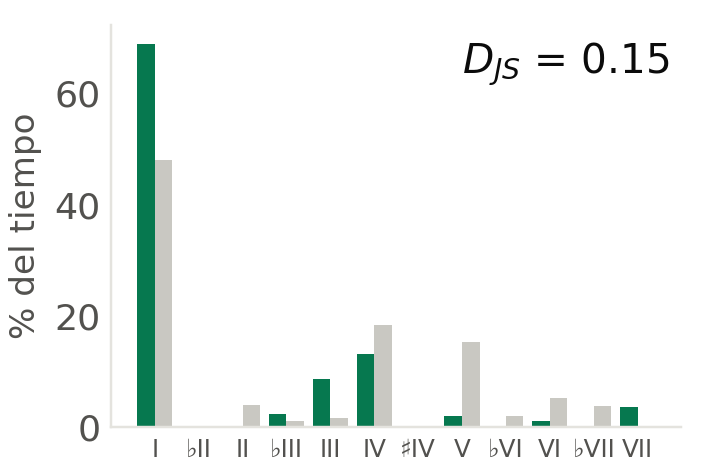
\includegraphics[width=\linewidth]{formula_js.png}
    \caption{Jensen-Shannon. Verde: fundamentales de «My Name Is Mud»; gris: centro del rock ($D_{\mathrm{JS}}=0.15$).}
  \end{subfigure}\hfill
  \begin{subfigure}{0.48\textwidth}\centering
    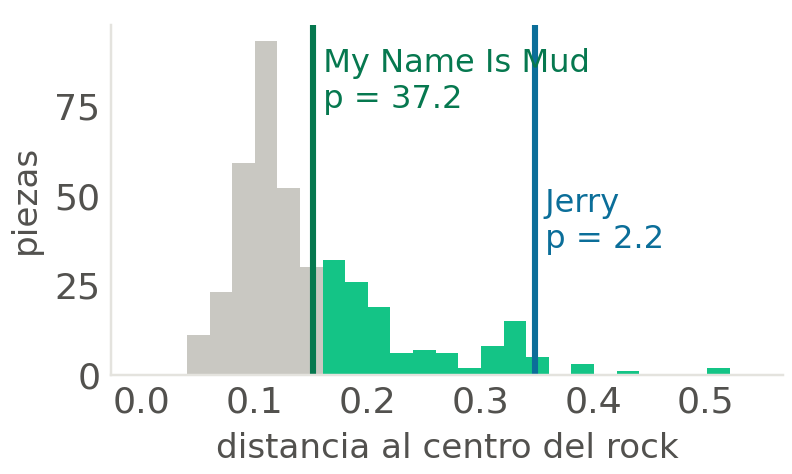
\includegraphics[width=\linewidth]{formula_percentil.png}
    \caption{Percentil. Gris: distancias de las piezas de rock a su centro; verde: las más lejanas que «My Name Is Mud» ($p=37.2$).}
  \end{subfigure}\\[0.8em]
  \begin{subfigure}{0.48\textwidth}\centering
    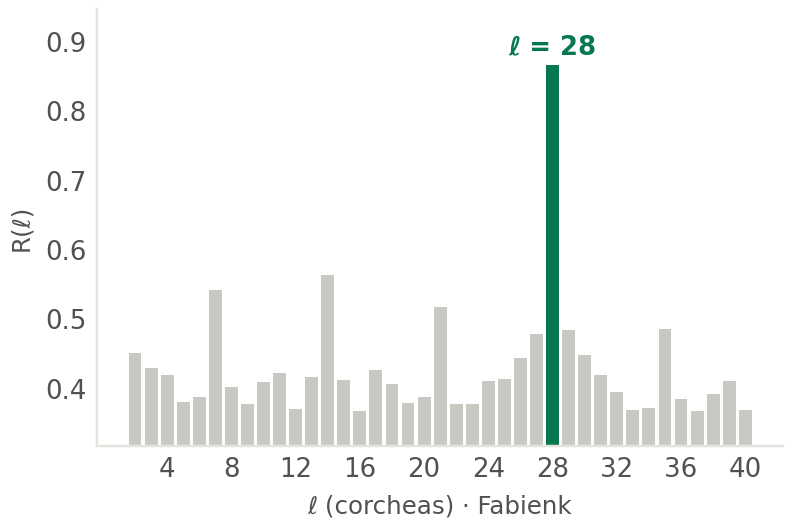
\includegraphics[width=\linewidth]{formula_repeticion.png}
    \caption{Repetición: $R(\ell)$ de «Jerry Was a Race Car Driver»; el pico en 8 corcheas es un compás de 4/4.}
  \end{subfigure}\hfill
  \begin{subfigure}{0.48\textwidth}\centering
    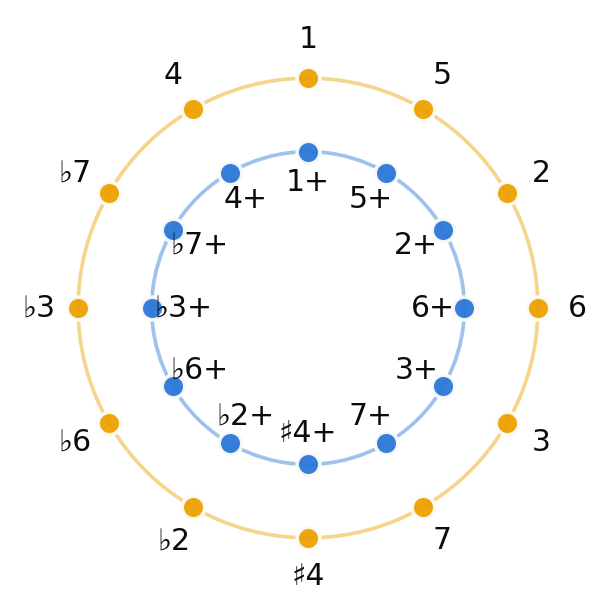
\includegraphics[width=\linewidth]{formula_campos.png}
    \caption{Los dos campos de quintas de 24-EDO: amarillo, el regular; azul, el de cuarto de tono.}
  \end{subfigure}
  \caption{Las medidas de comparación, ilustradas con canciones de Primus.}\label{fig:formulas}
\end{figure}

Las propiedades anteriores se deducen de la entropía de Shannon, $H(P) = -\sum_i P_i \log_2 P_i$ (con $0 \log 0 = 0$),
que mide en bits qué tan repartida está una distribución.

\begin{proposicion}[Desigualdad de Gibbs]
Para dos distribuciones $P$ y $Q$ sobre el mismo conjunto finito, $D_{\mathrm{KL}}(P \,\|\, Q) \ge 0$, con igualdad si y
solo si $P = Q$.
\end{proposicion}

\begin{proof}
Sea $I = \{i : P_i > 0\}$. Como $\log_2$ es cóncava, la desigualdad de Jensen da
\[
  -D_{\mathrm{KL}}(P \,\|\, Q) = \sum_{i \in I} P_i \log_2 \frac{Q_i}{P_i}
  \le \log_2 \sum_{i \in I} P_i \frac{Q_i}{P_i} = \log_2 \sum_{i \in I} Q_i \le \log_2 1 = 0.
\]
La igualdad en Jensen exige que $Q_i / P_i$ sea constante en $I$, y la segunda, que $\sum_{i \in I} Q_i = 1$; juntas
implican $P = Q$.
\end{proof}

\begin{proposicion}[Propiedades de Jensen-Shannon]\label{prop:js}
Para todo par de distribuciones $P, Q$:
\begin{enumerate}
  \item $D_{\mathrm{JS}}(P, Q) = H(M) - \tfrac12 H(P) - \tfrac12 H(Q)$, con $M = \tfrac12 (P + Q)$;
  \item $D_{\mathrm{JS}}(P, Q) = D_{\mathrm{JS}}(Q, P)$, y $D_{\mathrm{JS}}(P, Q) = 0$ si y solo si $P = Q$;
  \item $0 \le D_{\mathrm{JS}}(P, Q) \le 1$, y vale 1 si y solo si $P$ y $Q$ tienen soportes disjuntos;
  \item $D_{\mathrm{JS}}$ siempre es finita, aunque $P$ o $Q$ tengan ceros.
\end{enumerate}
\end{proposicion}

\begin{proof}
(1) Desarrollando, $D_{\mathrm{KL}}(P \,\|\, M) = -H(P) - \sum_i P_i \log_2 M_i$, y lo mismo para $Q$. Al promediar, los
términos cruzados suman $-\sum_i M_i \log_2 M_i = H(M)$.
(2) La simetría es evidente en la definición. Por Gibbs, cada sumando es no negativo y se anula solo si $P = M$ y
$Q = M$, es decir, si $P = Q$.
(3) Como $M_i \ge \tfrac12 P_i$, se tiene $\log_2 (P_i / M_i) \le \log_2 2 = 1$, así que
$D_{\mathrm{KL}}(P \,\|\, M) \le \sum_i P_i = 1$, y lo mismo para $Q$; el promedio es a lo sumo 1. La igualdad exige
$M_i = \tfrac12 P_i$ siempre que $P_i > 0$, es decir, $Q_i = 0$ donde $P_i > 0$, y viceversa.
(4) Si $P_i > 0$ entonces $M_i > 0$, de modo que ningún cociente $P_i / M_i$ se indefine.
\end{proof}

Que $\sqrt{D_{\mathrm{JS}}}$ satisfaga además la desigualdad triangular, y sea por tanto una métrica, es un resultado
más delicado \citep{endres2003}; en este trabajo se usa solo para justificar que las distancias entre canciones se pueden
comparar de manera coherente.

\subsection{Percentil de tipicidad}

Una distancia sola no dice si una canción es normal dentro de un estilo. El \emph{percentil de tipicidad} la compara con
las distancias de las propias piezas del corpus.

\begin{definicion}[Percentil de tipicidad respecto del centro]
Sea $C$ un corpus, $c$ su centro (el reparto promedio) y $d(x) = D_{\mathrm{JS}}(x, c_{-x})$ la distancia de cada pieza
al centro de las demás. Para una canción $s$,
\[
  p(s) = 100 \cdot \frac{\#\{x \in C : d(x) \ge d(s)\}}{|C|}.
\]
\end{definicion}

Un valor de 50 corresponde a una pieza típica del estilo; 0, a una canción más rara que todas las piezas del corpus.
«My Name Is Mud» da 37 en el rock y «Jerry Was a Race Car Driver», 2.2. Esta versión se usa en la matriz de armonía.

Un estilo puede tener varias zonas: un corpus con 93\,\% de piezas en 4 y 7\,\% en 3 tiene un promedio «en 4 con un poco
de 3» que no se parece a ninguna pieza. Por eso, en el test por bloques, la tipicidad se mide con vecinos.

\begin{definicion}[Percentil de tipicidad por vecinos]
Sea $d_k(s)$ la distancia de $s$ a su $k$-ésima pieza más cercana del corpus ($k = 5$). Para cada pieza $x \in C$ se
calcula $d_k(x)$ sin contarse a sí misma (ni a otra versión de la misma canción). Entonces
\[
  p_k(s) = 100 \cdot \frac{\#\{x \in C : d_k(x) \ge d_k(s)\}}{|C|}.
\]
\end{definicion}

\subsection{Percentil y significancia}

El percentil de tipicidad se puede leer como un valor $p$ empírico, y eso justifica el umbral de 5 que usa el veredicto.

\begin{proposicion}\label{prop:percentil}
Sea $C = \{x_1, \dots, x_n\}$ un corpus y $s$ una pieza nueva. Si $d(s), d(x_1), \dots, d(x_n)$ son intercambiables (por
ejemplo, si $s$ y las piezas del corpus provienen del mismo estilo) y no hay empates, entonces, para todo $u \in [0, 100]$,
\[
  \Pr\bigl[p(s) \le u\bigr] \le \frac{\lfloor u n / 100 \rfloor + 1}{n + 1} \approx \frac{u}{100}.
\]
\end{proposicion}

\begin{proof}
Por intercambiabilidad, el rango de $d(s)$ entre los $n + 1$ valores es uniforme en $\{1, \dots, n+1\}$. El percentil
$p(s)$ es $100/n$ veces el número de piezas del corpus con distancia mayor o igual; $p(s) \le u$ equivale a que a lo sumo
$\lfloor u n / 100 \rfloor$ piezas superen a $s$, es decir, a que $d(s)$ esté entre los $\lfloor u n / 100 \rfloor + 1$
valores más grandes. Esa probabilidad es $(\lfloor u n/100 \rfloor + 1)/(n + 1)$.
\end{proof}

En palabras: una pieza auténtica del estilo cae por debajo del percentil 5 alrededor del 5\,\% de las veces. Por eso el
umbral $u = 5$ funciona como un contraste a una cola con nivel 5\,\%, y la calibración del capítulo~\ref{cap:resultados}
(5.2\,\% de «sin vecino» en piezas reales de rock) lo confirma empíricamente.

\subsection{Distancia de Hellinger y componentes principales}

Para dibujar en un plano los repartos de fundamentales (vectores de 12 componentes) se usa el análisis de componentes
principales sobre la raíz cuadrada de cada reparto. La raíz tiene una justificación geométrica.

\begin{proposicion}\label{prop:hellinger}
La aplicación $P \mapsto \sqrt{P} = (\sqrt{P_1}, \dots, \sqrt{P_n})$ lleva el símplex de distribuciones a la esfera
unitaria de $\mathbb{R}^n$, y
\[
  \bigl\| \sqrt{P} - \sqrt{Q} \bigr\|_2^2 = 2 \Bigl(1 - \sum_i \sqrt{P_i Q_i}\Bigr) = 2\, H^2(P, Q),
\]
donde $H(P, Q)$ es la distancia de Hellinger. Es decir, la distancia euclidiana entre las raíces es (salvo el factor
$\sqrt2$) una distancia entre distribuciones, que además da más peso relativo a las diferencias en los grados poco usados
que la distancia euclidiana entre las distribuciones mismas.
\end{proposicion}

\begin{proof}
$\|\sqrt{P}\|_2^2 = \sum_i P_i = 1$. Desarrollando el cuadrado,
$\|\sqrt{P} - \sqrt{Q}\|^2 = \sum_i P_i + \sum_i Q_i - 2 \sum_i \sqrt{P_i Q_i} = 2 - 2 \sum_i \sqrt{P_i Q_i}$. Para la
última afirmación, $(\sqrt{a} - \sqrt{b})^2 = (a - b)^2 / (\sqrt a + \sqrt b)^2$, que crece cuando $a$ y $b$ son pequeños.
\end{proof}

El análisis de componentes principales busca, sobre los vectores centrados $y_k = \sqrt{P^{(k)}} - \bar y$ de las piezas de
los corpus, las direcciones de máxima varianza.

\begin{proposicion}\label{prop:pca}
Sea $Y$ la matriz cuyas filas son los $y_k$, y $Y = U \Sigma V^{\top}$ su descomposición en valores singulares, con
$\sigma_1 \ge \sigma_2 \ge \dots$. Entre los vectores unitarios $w$, la varianza de la proyección, $\|Yw\|^2$, es máxima
para $w = v_1$; entre los unitarios ortogonales a $v_1$, es máxima para $w = v_2$.
\end{proposicion}

\begin{proof}
$\|Yw\|^2 = w^{\top} Y^{\top} Y w = w^{\top} V \Sigma^2 V^{\top} w = \sum_j \sigma_j^2 (v_j^{\top} w)^2$. Como
$\sum_j (v_j^{\top} w)^2 = \|w\|^2 = 1$, la suma es un promedio ponderado de los $\sigma_j^2$, máximo cuando todo el peso
está en $j = 1$. Restringido a $w \perp v_1$, el peso de $j = 1$ es cero y el máximo se alcanza en $v_2$.
\end{proof}

Cada eje del mapa es una componente principal $v_j$: la dirección en la que más se diferencian las piezas de los corpus.
Las canciones de la banda se proyectan sobre los ejes obtenidos con los corpus, sin participar en su cálculo; así su
posición se lee en las coordenadas de los estilos y no altera el mapa. Las componentes con más peso en cada eje se
indican en la figura.

\subsection{Repetición a distancia \texorpdfstring{$\ell$}{l}}

Para encontrar el ciclo métrico se compara la música consigo misma $\ell$ corcheas después. Si $c_t$ es la clase de
altura de la voz aguda en la corchea $t$ y $a_t \in [0,1]$ la intensidad de ataque,
\[
  R(\ell) = 0.7\, \Pr\!\left[c_t = c_{t+\ell}\right] + 0.3 \left(1 - \overline{|a_t - a_{t+\ell}|}\right).
\]
Un pico alto y aislado en $R$ indica un ciclo largo y estable; un ciclo verdadero de $L$ corcheas da picos en $L$ y en
sus múltiplos. Por ejemplo, «Jerry Was a Race Car Driver» se repite cada 8 corcheas: un compás de 4/4.

\subsection{Medida F}

Para evaluar una transcripción se compara cada nota detectada con las de la referencia. La \emph{precisión} $P$ es la
fracción de notas detectadas que son correctas y la \emph{exhaustividad} $E$, la fracción de notas de la referencia que se
encontraron. La medida F es su media armónica \citep{vanrijsbergen1979}:
\[
  F = \frac{2PE}{P + E}.
\]
En este trabajo, una nota es correcta si su ataque cae a $\pm 75$~ms del de la referencia y su altura en la misma casilla
de 24-EDO ($\pm 25$ cents).

\chapter{Estado del arte}\label{cap:estado}

El análisis computacional de la música ofrece un marco cuantificable para estudiar la melodía, la armonía, el ritmo y el
timbre, y resulta especialmente útil frente a músicas que desafían los modelos teóricos convencionales. La
microtonalidad, el uso de intervalos menores que el semitono, es uno de esos casos: la notación occidental y la mayoría
de las herramientas de análisis no representan con precisión las alturas que caen entre los semitonos.

Este trabajo toma elementos de seis líneas de investigación. La tabla~\ref{tab:estado} resume, para cada una, qué
resuelve, qué le falta para esta música y qué se usa aquí.

\begin{table}[ht]
  \centering\small
  \caption{Líneas de trabajo previo y su relación con este trabajo.}\label{tab:estado}
  \begin{tabularx}{\textwidth}{@{}>{\raggedright}p{2.2cm}>{\raggedright}p{3.1cm}>{\raggedright}X>{\raggedright}X>{\raggedright\arraybackslash}X@{}}
    \toprule
    Línea & Trabajos & Qué resuelven & Qué les falta aquí & En este trabajo \\
    \midrule
    Altura desde el audio & \citet{mauch2014}; \citet{bittner2022} & Melodía y notas a partir de la grabación &
      pYIN sigue una sola voz; Basic Pitch da notas MIDI enteras y el cuarto de tono queda como desafinación &
      Saliencia armónica y consenso entre vueltas del looper \\
    Separación de fuentes & \citet{rouard2023}; \citet{lu2024} & Aislar bajo, guitarra y batería &
      No transcriben: solo preparan la señal & Demucs para guitarra y bajo \\
    MIR microtonal & \citet{bozkurt2008}; \citet{gedik2010} & Histogramas de altura finos para el makam turco &
      Música de una sola voz, sin acordes ni looper & Rejilla de 24-EDO con casillas de $\pm25$ cents \\
    Armonía funcional & \citet{riemann1893}; \citet{lendvai1971}; \citet{piston1987} &
      Función de cada acorde: tónica, subdominante o dominante & Pensada en 12 notas; Piston deja fuera lo microtonal &
      Calidades, funciones y ejes extendidos a 24-EDO \\
    Estilo con corpus & \citet{declercq2011}; \citet{broze2013} & Perfiles de armonía del rock y del jazz &
      Datos simbólicos en 12 notas & Perfiles de 24 clases, Jensen-Shannon y percentil \\
    Métrica irregular & \citet{holzapfel2014}; \citet{srinivasamurthy2016} & Compases no occidentales desde el audio &
      Sin la dimensión de altura & Pulsos y compases de 2 a 8 pulsos \\
    \bottomrule
  \end{tabularx}
\end{table}

\section{Altura desde el audio}

Los estimadores de frecuencia fundamental como YIN \citep{decheveigne2002} y pYIN \citep{mauch2014} siguen con precisión
una línea monofónica y entregan alturas continuas que pueden expresarse como MIDI fraccionario o desviación en cents. Los
modelos de redes neuronales, como CREPE \citep{kim2018}, mejoran la estimación en una sola voz. Para música polifónica, la
extracción de melodía basada en contornos de saliencia \citep{salamon2012} y los transcriptores multinota, como Basic Pitch
\citep{bittner2022}, entregan varias notas a la vez, pero cuantizadas a doce notas: un cuarto de tono les sale como una
nota desafinada.

\section{Separación de fuentes}

Demucs \citep{rouard2023} y BS-RoFormer \citep{lu2024} separan una mezcla en pistas de instrumentos (bajo, batería, voz,
guitarra y otros). Son un paso previo útil, pero no transcriben. REPET \citep{rafii2013} separa lo que se repite de lo
que no, una idea cercana al funcionamiento de un looper.

\section{MIR microtonal}

El estudio computacional del makam turco ha desarrollado histogramas de altura de alta resolución y comparaciones entre
modelos teóricos de afinación y mediciones \citep{bozkurt2008,bozkurt2009,gedik2010,bozkurt2014}. Estas técnicas trabajan
con música de una sola voz (heterofonía, en el mejor de los casos), sin acordes y sin la estructura en capas de un
looper. \citet{serra2011} propuso un enfoque multicultural para la investigación en información musical: los modelos
del área se construyeron sobre la música occidental y tienden a llevar ese sesgo a otras tradiciones.

\section{Armonía funcional}

Las teorías de \citet{riemann1893}, \citet{lendvai1971} y \citet{piston1987} clasifican los acordes por su función
tonal. Todas están pensadas para doce notas, y Piston excluye explícitamente las escalas microtonales.

\section{Estilo con corpus}

Los estudios de corpus describen estadísticamente la armonía de un estilo: el rock \citep{declercq2011,temperley2013},
la práctica común \citep{temperley2009} y el jazz \citep{broze2013,shanahan2012}. La comparación de distribuciones con
medidas de teoría de la información tiene base en la cognición musical \citep{krumhansl1990,huron2006,pearce2018}. Todos
estos corpus son simbólicos y están en doce notas.

\section{Métrica irregular}

El seguimiento de compases no occidentales desde el audio, como los usul turcos o los tala indios, se ha estudiado con
modelos bayesianos \citep{holzapfel2014,srinivasamurthy2016}, y el seguimiento de pulsos por programación dinámica es un
método clásico \citep{ellis2007}. Estos trabajos no incorporan la dimensión de altura.

\section{El vacío}

Ningún trabajo consultado reúne a la vez audio polifónico, 24-EDO, armonía funcional y comparación con corpus. Este
trabajo une las seis líneas para estudiar una banda de rock con cuartos de tono y looper.

\chapter{Datos}\label{cap:datos}

\section{Conjuntos de canciones}

La tabla~\ref{tab:conjuntos} resume las canciones que se analizan con la herramienta. Todas se procesan con el mismo
cuaderno y los mismos parámetros, a partir del audio oficial.

\begin{table}[ht]
  \centering
  \caption{Canciones analizadas con la herramienta.}\label{tab:conjuntos}
  \begin{tabularx}{\textwidth}{@{}>{\raggedright}p{6.2cm}c>{\raggedright\arraybackslash}X@{}}
    \toprule
    Conjunto & Tamaño & Uso \\
    \midrule
    Angine de Poitrine, \emph{Vol.~II} & 6 temas & Objeto de estudio (audio oficial) \\
    Referencias corregidas de oído & 4 temas & Evaluación; Yor Zarad, a ciegas \\
    Primus & 3 temas & Control sin cuartos de tono: mide el error \\
    King Gizzard, \emph{Flying Microtonal Banana} (2017) & 9 temas & Rock en 24-EDO (precedente señalado por analistas) \\
    Zappa / King Crimson / Gentle Giant & 6 / 6 / 6 & Rock progresivo comparado \\
    \bottomrule
  \end{tabularx}
\end{table}

En total se midieron 36 canciones: las 6 del álbum, los 3 controles de Primus y 27 de los repertorios comparados. Las
referencias de oído son de canciones del álbum, así que no suman al total.

Las seis canciones del álbum son Mata Zyklek, Fabienk, Sarniezz, Yor Zarad, Utzp y Angor. Los controles de Primus son
«Tommy the Cat», «My Name Is Mud» y «Jerry Was a Race Car Driver». Primus cumple dos papeles: es la comparación propia
del trabajo y, como no usa cuartos de tono, todo cuarto de tono que la herramienta marque en sus canciones es error de
medición. Con él se estima el \emph{piso de ruido} de la herramienta.

\section{Referencias para medir el acierto}\label{sec:referencias}

Para saber si la herramienta acierta se necesitan transcripciones verificadas. Se armaron cuatro:

\begin{itemize}
  \item \textbf{Sarniezz y Fabienk.} Partituras de Guitar Pro y MuseScore, corregidas de oído por el autor. Cada
  corrección se verificó con clips: la pista de guitarra real en un canal y la partitura sintetizada en el otro.
  \item \textbf{Mata Zyklek.} La transcripción de la sesión de KEXP, sin cambios en la primera ronda.
  \item \textbf{Yor Zarad.} La primera referencia armada sin mirar ninguna salida de la herramienta: las alturas salen de
  la tablatura de los PDF de Guitar Pro y los tiempos, de los audios que Guitar Pro exporta por pista. El autor la
  verificó de oído con 20 clips y eligió a ciegas entre versiones en 6 clips más.
\end{itemize}

Además, para Sarniezz, Mata Zyklek y Fabienk se armó una referencia de acordes con \emph{todas} las pistas de la partitura
de Guitar Pro (guitarras I a VI y bajo), ya alineadas al tiempo de la grabación oficial. Solo sirve para evaluar la
armonía (sección~\ref{sec:evaluacion}).

Las partituras publicadas no se usan nunca para guiar el análisis: la herramienta tiene que funcionar con canciones sin
partitura. Utzp era una segunda prueba a ciegas, pero su referencia no pasó la verificación de oído (el ritmo de las
guitarras de acordes) y se usó después como una canción más.

\section{Corpus de estilos}\label{sec:corpus}

La tabla~\ref{tab:corpus} muestra los seis corpus que entran en la comparación final. Cada uno aporta los bloques de
rasgos que tiene.

\begin{table}[ht]
  \centering\small
  \caption{Corpus de estilos usados en la comparación.}\label{tab:corpus}
  \begin{tabularx}{\textwidth}{@{}l>{\raggedright}Xlr@{}}
    \toprule
    Estilo & Corpus & Bloques & Piezas \\
    \midrule
    Rock & Rolling Stone 200 \citep{declercq2011} & armonía, escala, metro & 200 (400 análisis) \\
    Práctica común & Kostka-Payne \citep{temperley2009} & armonía & 46 \\
    Jazz & iRealPro \citep{irealpro} & armonía, metro & 1\,186 \\
    Pop & 9 álbumes de Hooktheory & armonía & 121 \\
    Persa & Radif Corpus \citep{kanani2025} & escala, cuartos de tono & 229 \\
    Indostánica & Hindustani Classical Music Transcription Dataset \citep{singh2022} & escala, cuartos de tono & 50 \\
    \bottomrule
  \end{tabularx}
\end{table}

El corpus de rock contiene las 200 canciones de la lista de la revista Rolling Stone, analizadas por dos analistas (400
análisis). El de práctica común proviene de los ejemplos del libro de armonía de Kostka y Payne y solo tiene armonía. El
de jazz reúne los acordes de los estándares de la aplicación iRealPro. El de pop son 121 temas de 9 álbumes analizados
en Hooktheory (Adele, Reneé Rapp, Luke Combs, Billie Eilish, Taylor Swift, Lil Nas X, Lorde, Ed Sheeran y Tate McRae)
\citep{hooktheory}. El
radif es el repertorio clásico de la música persa, organizado en modos (\emph{dastgah}), con intervalos menores que el
semitono (\emph{koron} y \emph{sori}); la conversión del proyecto da 229 piezas \citep{kanani2025}. El corpus indostánico
trae alturas en 22 \emph{shrutis}, que al llevarse a 24-EDO caen todas en los doce grados regulares.

\paragraph{Descargados pero no usados.} SymbTr (makam turco, unas 2\,200 piezas con alturas en comas de Holder)
\citep{karaosmanoglu2012} y The Session (folk irlandés) se convirtieron a bloques y se retiraron de la comparación
final. El maqam árabe no tiene un corpus simbólico abierto equivalente. ProgGP \citep{loth2023}, el corpus que permitiría
comparar con el rock progresivo, solo se obtiene pidiéndolo a sus autores y no estuvo disponible.

\paragraph{Corpus pequeños.} Solo cuentan para el veredicto los corpus con 100 piezas o más. En un corpus pequeño y
disperso casi todo parece típico; en las figuras, las comparaciones con corpus de menos de 100 piezas (Kostka-Payne e
indostánico) aparecen rayadas.

\section{Fuentes sobre la banda}

Las declaraciones de la banda se documentan con la entrevista de \emph{Noize Magazine} \citep{noize} y el podcast
\emph{Aucard de Tours} \citep{aucard2026}. Del podcast se usó una transcripción de trabajo, no oficial, del tramo
1:33--2:58, en la que Khn describe el dúo de guitarra y bajo microtonales, la construcción por loops, la repetición con
crescendo, la relación estructural con el techno, la tradición del rock instrumental y el uso de 5 y 7 tiempos. Los
análisis externos provienen de los videos de Mathémusique \citep{mathemusique2026}, David Bennett \citep{bennett2026},
Levi McClain \citep{mcclain2026} y Thomas Little \citep{little2019}. La prensa \citep{weller2026,dunlevie2026} se usó
solo para los datos generales de la banda y del instrumento.

\section{Licencias}

El audio de la banda no se distribuye. Los corpus conservan la licencia de su fuente; el repositorio publica agregados,
huellas, scripts y referencias, y no los conjuntos completos cuando la licencia no lo permite. Los pesos de BS-RoFormer
SW no declaran licencia y se usaron solo con fines académicos.

\chapter{Metodología}\label{cap:metodologia}

El método final no fue el primero. Este capítulo cuenta primero cómo evolucionó (secciones~\ref{sec:idea-inicial}
a~\ref{sec:idea-tabroll}), porque cada cambio respondió a algo que mostró el audio. Después describe el algoritmo final
(sección~\ref{sec:algoritmo}), las decisiones sobre la melodía y la armonía, la evaluación y la comparación con estilos.

\section{La idea inicial y lo que mostró el audio}\label{sec:idea-inicial}

El trabajo partió de cuatro supuestos, y cada uno se puso a prueba contra el audio
(tabla~\ref{tab:supuestos}).

\begin{table}[ht]
  \centering\small
  \caption{Supuestos iniciales y cómo se pusieron a prueba.}\label{tab:supuestos}
  \begin{tabularx}{\textwidth}{@{}>{\raggedright}X>{\raggedright\arraybackslash}X@{}}
    \toprule
    Supuesto & Cómo se puso a prueba \\
    \midrule
    Los cuartos de tono solo aparecen en una zona del mástil: la parte más aguda como $\mathbb{Z}_{24}$ y el resto como
    $\mathbb{Z}_{12}$. & Medir cada nota sin decidir antes dónde puede haber cuartos de tono. \\
    La partitura publicada sirve como referencia principal para medir la precisión. & Escucharla frente a fragmentos de
    la grabación. \\
    Basta con pYIN para obtener la melodía. & Seguir con pYIN el bajo de Sarniezz. \\
    Las secciones de la canción se reconocen por el timbre. & Resumir el timbre de cada fragmento con MFCC y entrenar una
    red neuronal pequeña para reconocer la sección. \\
    \bottomrule
  \end{tabularx}
\end{table}

El primer supuesto se formalizó como una cuantización a trozos según el índice de traste $k$: los trastes de cuarto de
tono hasta una posición $k_0$ y de semitono a partir de ella,
\[
  f(k) =
  \begin{cases}
    f_0 \cdot 2^{k/24}, & k \le k_0, \\
    f(k_0) \cdot 2^{(k - k_0)/12}, & k > k_0,
  \end{cases}
\]
inspirada en el instrumento de Khn: la guitarra tiene 30 trastes de cuarto de tono seguidos de 6 de semitono, y el bajo,
24 de cuarto de tono seguidos de 6 de semitono. \pv[: número de trastes de cada instrumento] El método final no presupone
esa división: mide cada nota en la rejilla completa de 24-EDO.

El punto de partida fue la transcripción de Sarniezz en MuseScore, leída como piano roll en un primer cuaderno de Python
(figura~\ref{fig:primer-cuaderno}).

\begin{figure}[htbp]
  \centering
  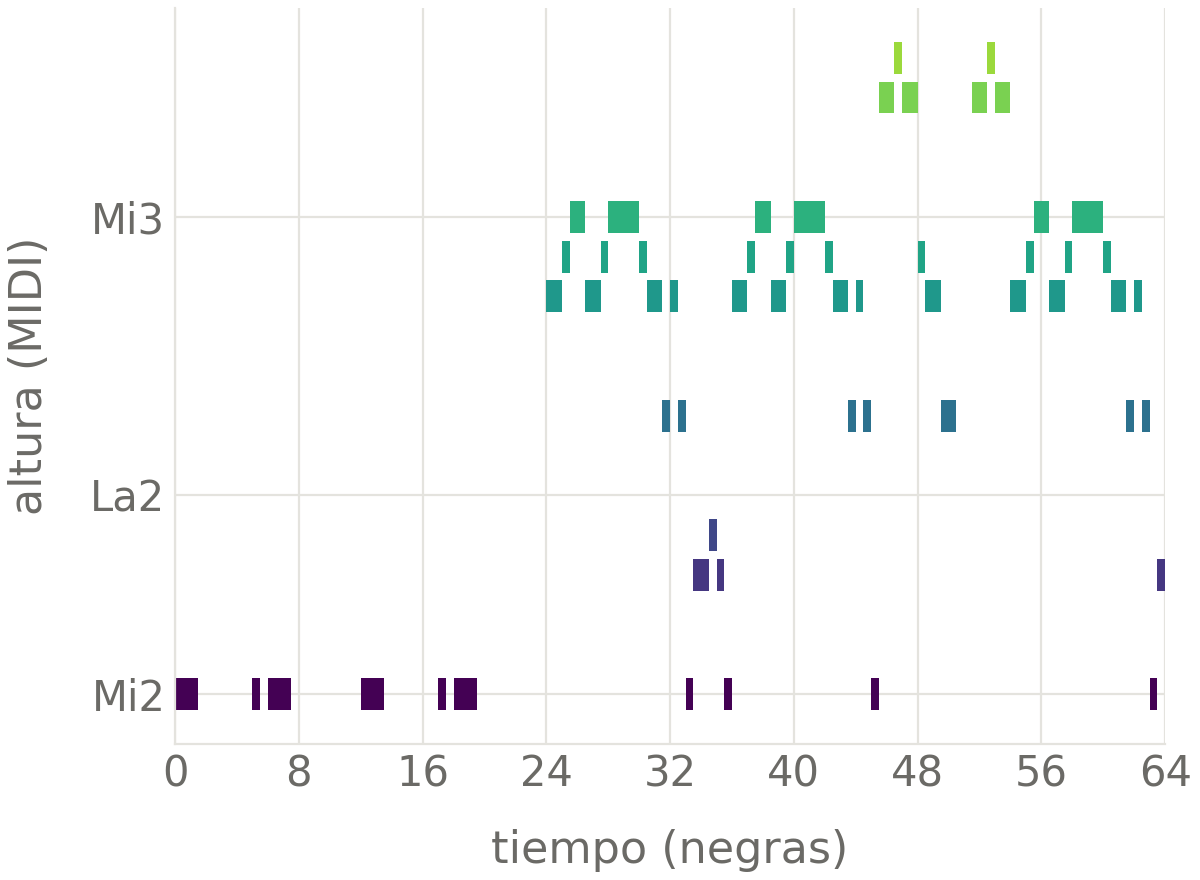
\includegraphics[width=0.75\textwidth]{cuaderno_original_sarniezz.png}
  \caption{Primer cuaderno: la partitura de Sarniezz en piano roll (primeras 64 negras). Aún no se medía el audio.}
  \label{fig:primer-cuaderno}
\end{figure}

\section{El primer algoritmo y por qué no bastó}\label{sec:primer-algoritmo}

El primer algoritmo tomó la pista de bajo de Sarniezz y le aplicó pYIN (de Do2 a Do7, ventana de 2048 muestras), que da
una altura por instante. Después midió la desviación en cents respecto del semitono más cercano. Por último, una red
neuronal intentó reconocer la sección de la canción a partir del timbre: 28 fragmentos del bajo de Sarniezz (27 de 10~s
y uno de 9.1~s), etiquetados a mano en seis secciones; 13 MFCC por fragmento, resumidos en su media y su desviación (26
números); un perceptrón de dos capas ocultas (64 y 32 neuronas) con partición estratificada de 21 fragmentos de
entrenamiento y 7 de prueba.

Las tres pruebas mostraron límites (figura~\ref{fig:primer-algoritmo}):
\begin{itemize}
  \item En el álbum suenan varias capas del looper al mismo tiempo, y pYIN, que solo ve una, salta de una a otra: no separa
  las voces ni da acordes.
  \item La desviación respecto del semitono más cercano siempre cae entre $-50$ y $+50$ cents. Un cuarto de tono queda
  justo en el borde y no se distingue de una nota desafinada.
  \item La red acertó 3 de 7 fragmentos (43\,\%). Con 21 ejemplos para seis secciones, y un timbre del bajo casi igual
  en toda la canción, los MFCC no bastan para reconocer la sección.
\end{itemize}

\begin{figure}[htbp]
  \centering
  \begin{subfigure}{\textwidth}\centering
    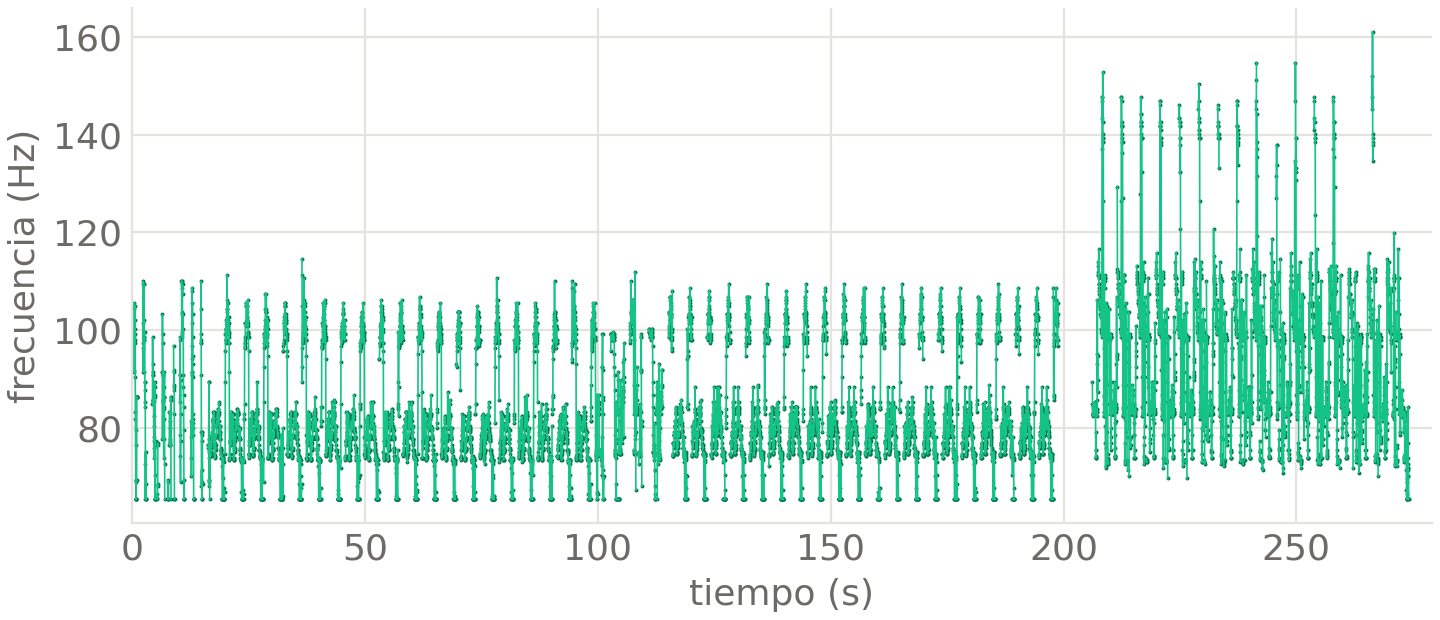
\includegraphics[width=0.8\linewidth]{original_pyin.png}
    \caption{pYIN da una sola altura por instante: no ve acordes.}
  \end{subfigure}\\[0.6em]
  \begin{subfigure}{0.6\textwidth}\centering
    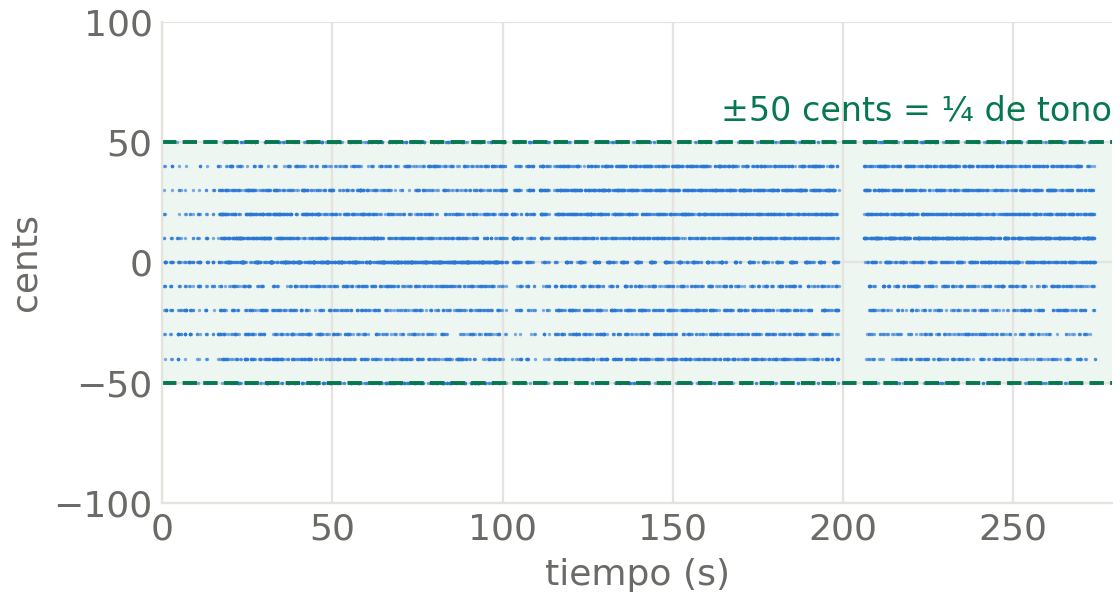
\includegraphics[width=\linewidth]{original_cents.png}
    \caption{La desviación del semitono nunca pasa de $\pm50$ cents: el cuarto de tono queda ambiguo.}
  \end{subfigure}\hfill
  \begin{subfigure}{0.36\textwidth}\centering
    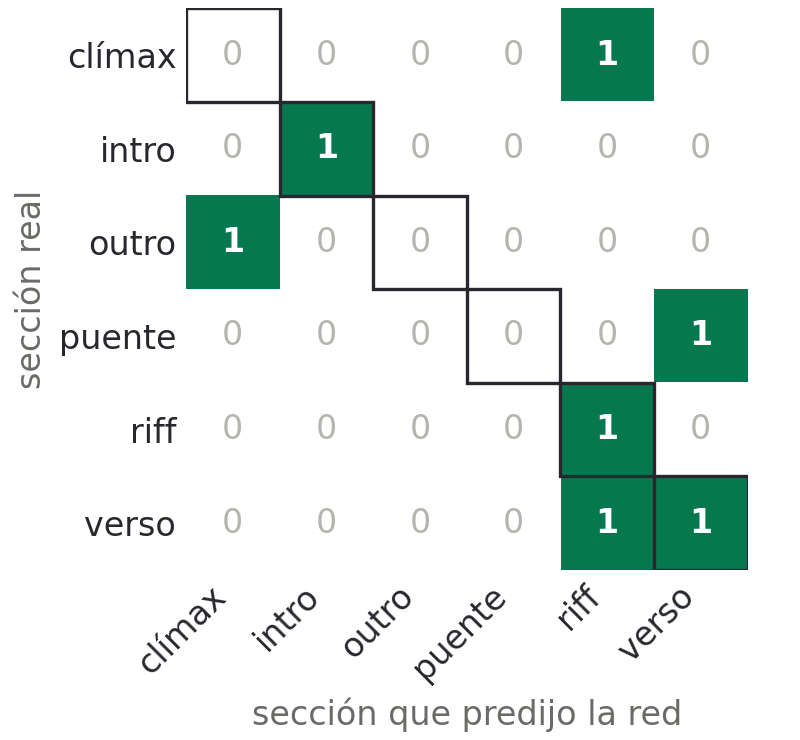
\includegraphics[width=\linewidth]{original_secciones_mlp.png}
    \caption{Matriz de confusión de la red por sección: acierta 3 de 7.}
  \end{subfigure}
  \caption{Primer algoritmo: por qué no bastó.}\label{fig:primer-algoritmo}
\end{figure}

Además, la partitura publicada resultó no ser un criterio fiable: también se equivoca, y la de Fabienk corresponde a la
versión en vivo. La conclusión fue que había que pasar de describir la señal a \emph{transcribir} notas, compases y
acordes, y que la referencia tenía que corregirse de oído.

El cuaderno empezó en Google Colab y pasó a un repositorio de GitHub cuando la memoria disponible dejó de alcanzar.

\section{La idea del tabroll}\label{sec:idea-tabroll}

Al estudiar la armonía de Primus se encontró el formato de Hooktheory \citep{hooktheory}: fragmentos de canciones transcritos a mano en un
piano roll dividido por compases, con la melodía arriba y el acorde de cada compás abajo. Hooktheory tiene una sola
canción de la banda, el riff de Fabienk, en doce notas por octava.

El \emph{tabroll} recrea esa idea con dos cambios: 24 filas por octava, para que los cuartos de tono tengan su lugar, y
generación automática desde el audio oficial de cualquier canción, sin transcribir nada a mano
(figura~\ref{fig:tabroll}). En el tramo de Fabienk de 4:42 a 4:52 (la melodía «Fabien»), la voz aguda del tabroll da la
misma nota que la partitura corregida el 78\,\% del tiempo, y 6 de sus 8 cuartos de tono están en la partitura.

\begin{figure}[htbp]
  \centering
  \begin{subfigure}{0.44\textwidth}\centering
    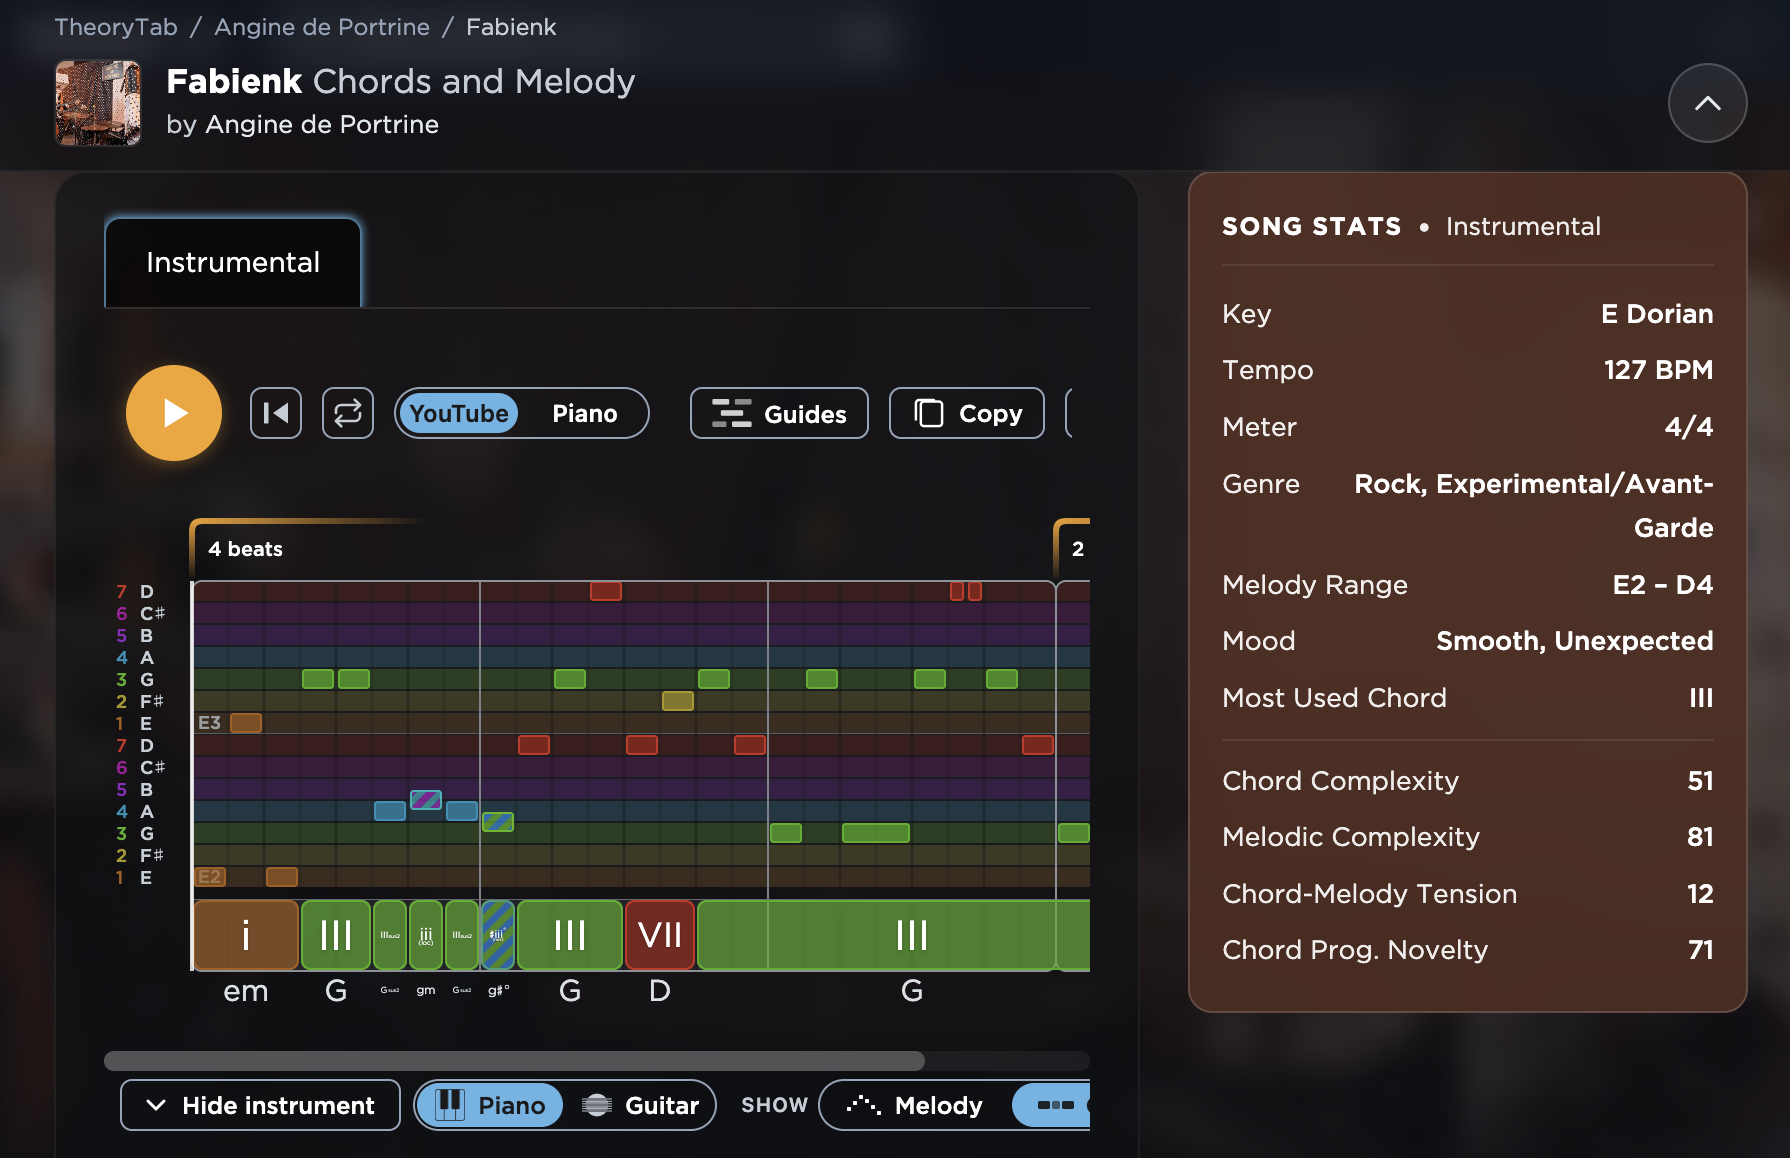
\includegraphics[width=\linewidth]{hooktheory_fabienk.png}
    \caption{Hooktheory (a mano): Mi dórico, 4/4, 12 notas.}
  \end{subfigure}\hfill
  \begin{subfigure}{0.53\textwidth}\centering
    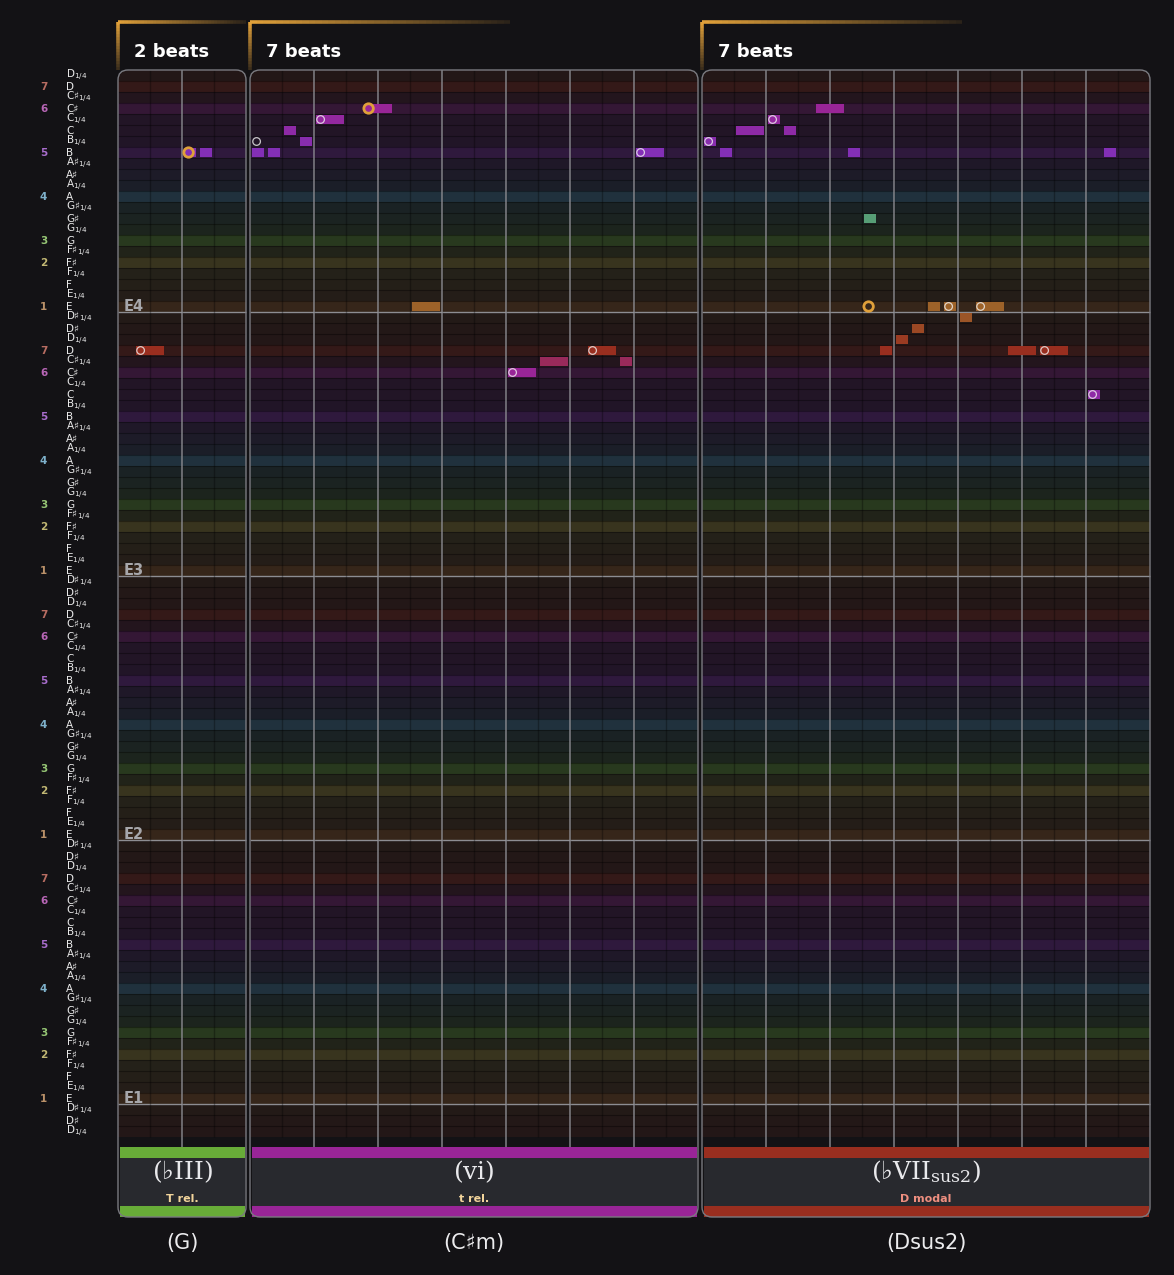
\includegraphics[width=\linewidth]{tabroll_fabienk.png}
    \caption{Tabroll desde el audio (4:42--4:52): los cuartos de tono, en las filas «+» azules.}
  \end{subfigure}
  \caption{De Hooktheory al tabroll: Fabienk en 12 notas y en 24.}\label{fig:tabroll}
\end{figure}

\section{Las primeras comparaciones con estilos}\label{sec:primeras-comparaciones}

La comparación con estilos también pasó por varias versiones antes del test por bloques.

\begin{enumerate}
  \item \textbf{Pop de Hooktheory.} La primera comparación fue con nueve álbumes de pop analizados en Hooktheory. La banda
  quedó lejos: a una distancia de Jensen-Shannon de 0.40 a 0.59, cuando los álbumes entre sí no pasan de 0.07.
  \item \textbf{Tarjetas al estilo de Hooktheory.} Las cinco métricas de Hooktheory son percentiles frente a su base de unas
  40\,000 canciones y no se pueden recalcular fuera de ella, así que se usaron valores crudos y las de Hooktheory solo
  como contexto. El resultado es una tarjeta por canción (figura~\ref{fig:tarjeta-mata}).
  \item \textbf{Pruebas de estilo con reglas.} Se definieron reglas con cifras publicadas para el rock, la práctica común,
  el jazz, la pentatónica, los tonos enteros, el dodecafonismo, el minimalismo y la música microtonal. Sirvieron para
  descartar: el jazz, la práctica común, los tonos enteros y el dodecafonismo no encajan en ninguna canción, y las
  fundamentales de la banda caen casi por completo en la pentatónica menor (del 86 al 100\,\% del tiempo). Pero los
  umbrales de las reglas los fijaba el autor, y eso era una debilidad. Los veredictos y las distancias de esta versión
  están en el apéndice (figuras~\ref{fig:g-distancias} a~\ref{fig:g-veredictos2}).
  \item \textbf{Matriz de verosimilitud.} Para no depender de umbrales propios, se pasó a ubicar cada canción dentro de la
  distribución real de cada estilo, con corpus: es la matriz de la sección~\ref{sec:comparacion}.
  \item \textbf{Radares.} Una figura de radar con una punta por estilo, separada en armonía, melodía y ritmo, resumía el
  perfil de cada canción (figura~\ref{fig:radar-mata}). La primera versión ponía cada punta en su propia escala, lo que
  impedía comparar puntas; se corrigió usando la verosimilitud.
  \item \textbf{Test por bloques.} Finalmente, la comparación se separó en bloques y se calibró con el error medido en
  Primus (sección~\ref{sec:comparacion}).
\end{enumerate}

\begin{figure}[htbp]
  \centering
  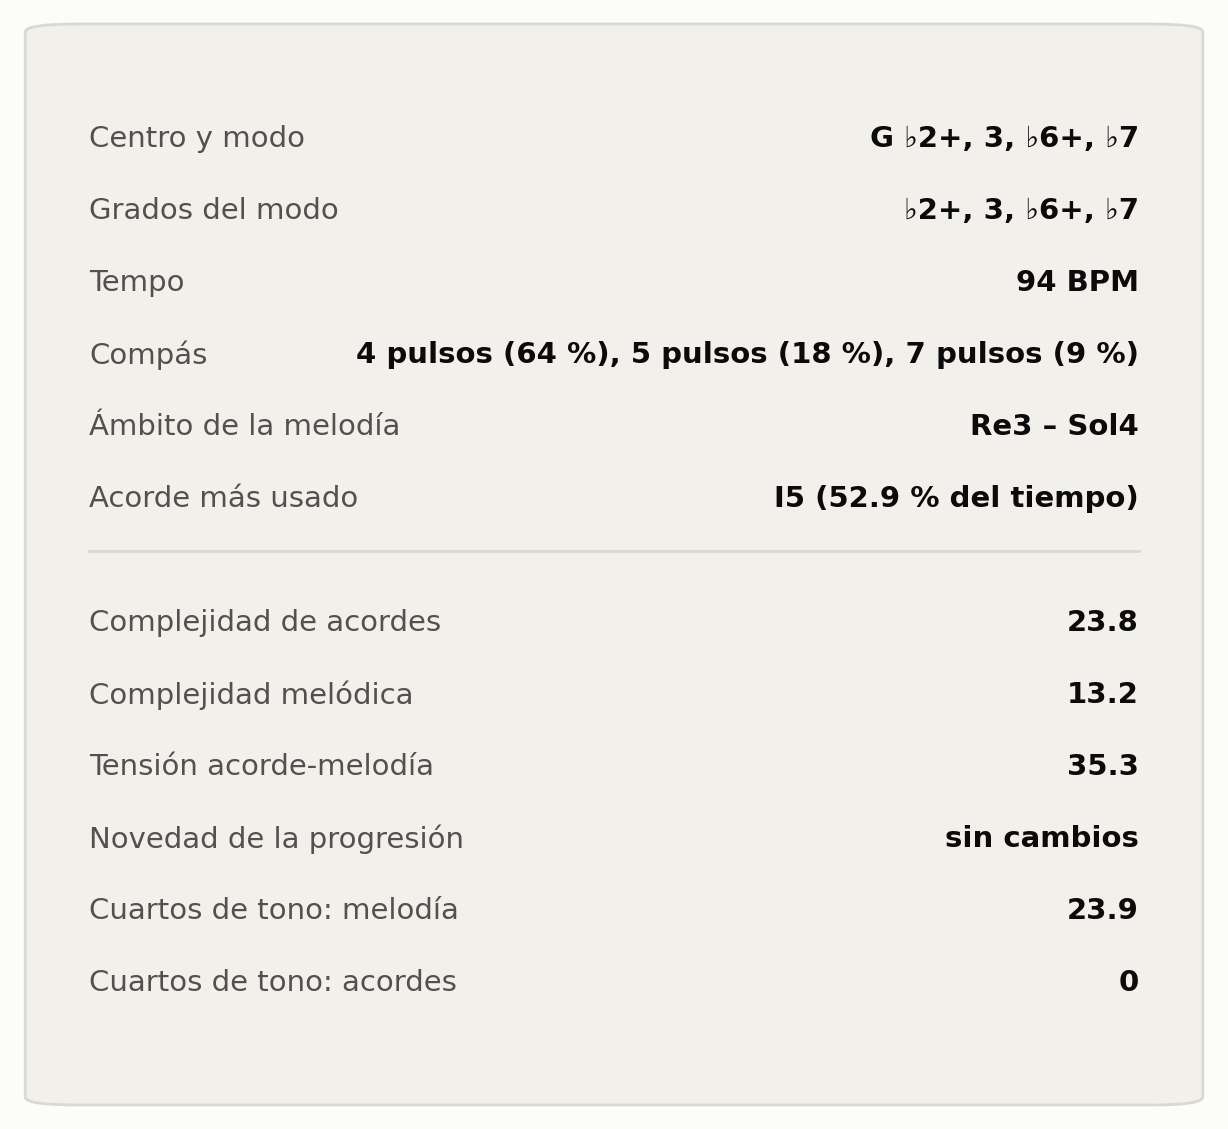
\includegraphics[width=0.5\textwidth]{mata_zyklek_tarjeta.png}
  \caption{Tarjeta de Mata Zyklek. Arriba, centro, modo, tempo, compases, ámbito y acorde más usado; abajo, seis métricas en valores crudos (0--100 o \% del tiempo; no son percentiles). Compases confiables: 78.3\,\% del tiempo; acierto contra la referencia: F 66.5 en la melodía y 95.4 en la fundamental.}\label{fig:tarjeta-mata}
\end{figure}

\begin{figure}[htbp]
  \centering
  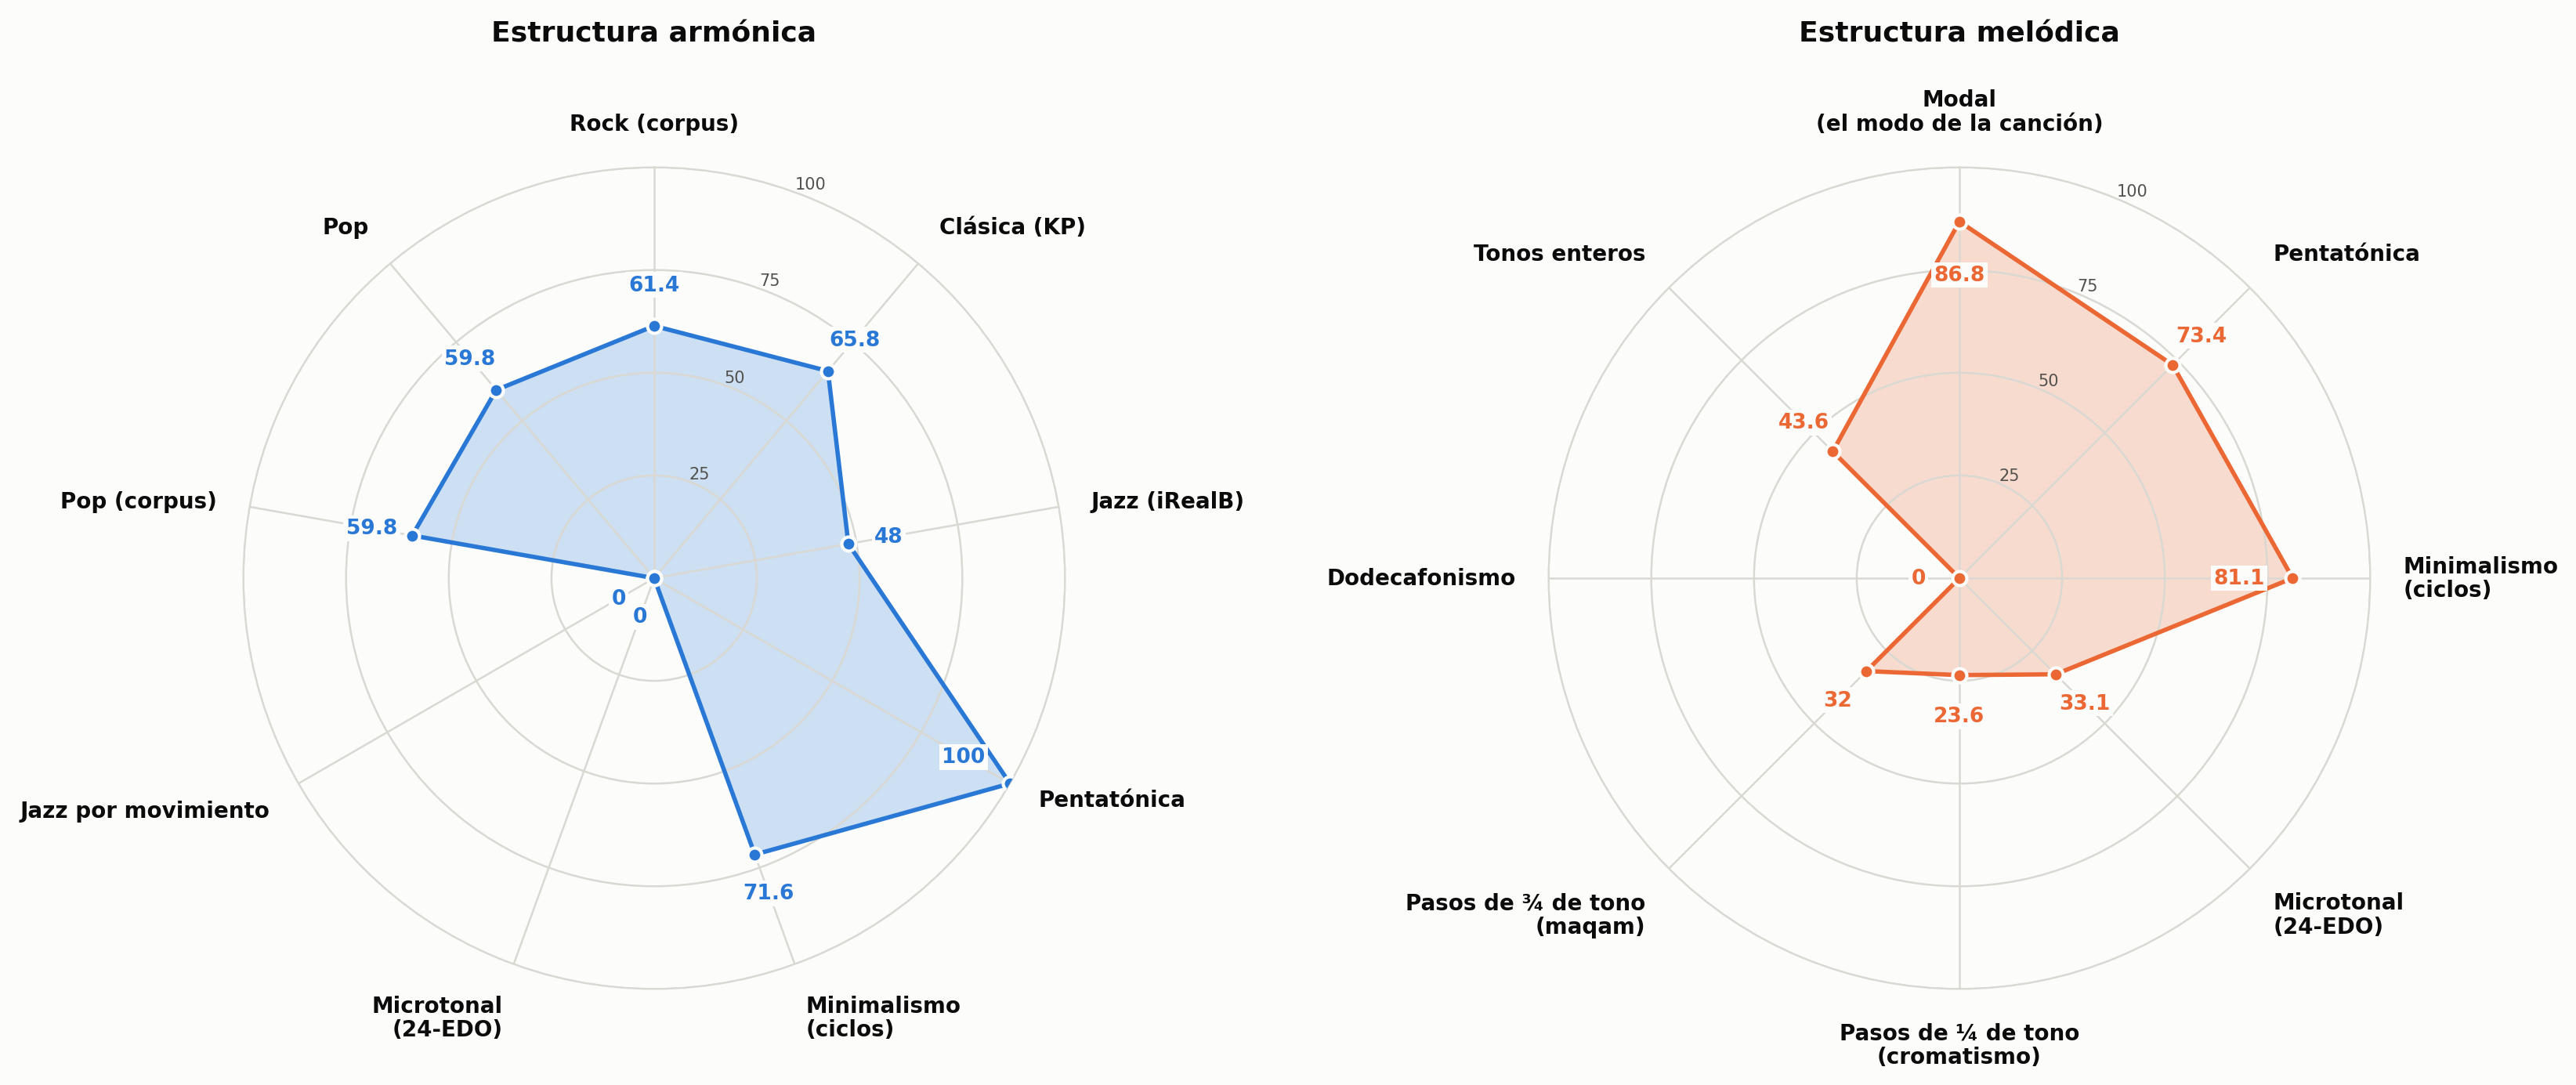
\includegraphics[width=\textwidth]{mata_zyklek_radar_estilos.png}
  \caption{Radar de estilos de Mata Zyklek (versión descartada, 15 de noviembre). Izquierda: armonía; derecha: melodía. Cada punta es un estilo en escala de 0 a 100: más lejos del centro, más parecido.}\label{fig:radar-mata}
\end{figure}

También la lectura de los cuartos de tono cambió. La primera versión medía solo la \emph{cantidad} de tiempo en cuartos
de tono, y la banda salía con poca microtonalidad, porque las fundamentales de los acordes casi nunca caen en cuarto de
tono. Después se intentó separar adorno de grado por la duración de la nota, pero Primus también daba «grados». Lo que sí
separa a la banda del control es la \emph{concentración} en pocos grados fijos (sección~\ref{sec:metodo-cuartos}).

\section{El algoritmo completo}\label{sec:algoritmo}

El algoritmo final tiene tres etapas (algoritmo~\ref{alg:tabroll}). La primera prepara la señal. La segunda, el núcleo
propio del trabajo, transcribe en 24-EDO guiada por el looper: como la banda repite cada riff, la altura se promedia entre
vueltas antes de decidir la nota, y por eso el método funciona con cuartos de tono. La tercera extrae la estructura y
compara con los estilos. La tabla~\ref{tab:parametros} da los parámetros, que vienen del código.

\begin{algorithm}[ht]
  \caption{TabRoll24($x$): del audio al veredicto de estilo.}\label{alg:tabroll}
  \KwIn{audio estéreo $x$}
  \KwOut{notas $N$ en 24-EDO, compases $B$, acordes $A$ y veredicto $V$ por bloque}
  \tcp{1 · Señal}
  $(g, b) \leftarrow \textsc{Separar}(x)$\tcp*{Demucs 6s, semilla 0}
  $S \leftarrow \textsc{Saliencia}(g, b)$\tcp*{10 armónicos, cada 25 cents}
  \tcp{2 · Núcleo: guiado por el looper}
  $\ell^* \leftarrow \textsc{Ciclo}(S)$\tcp*{autocorrelación, 1 a 16 s}
  $\hat S \leftarrow \textsc{Consenso}(S, \ell^*)$\tcp*{media en $\pm3$ vueltas}
  $w \leftarrow \textsc{Registro}(\hat S)$\tcp*{altura típica de la melodía}
  $m^* \leftarrow \textsc{Viterbi}(w \hat S)$\tcp*{contorno sin saltos innecesarios}
  $N \leftarrow \textsc{Notas}(m^*)$\tcp*{redondeo a \cuarto{} de tono}
  $N \leftarrow \textsc{Limpiar}(N, \ell^*)$\tcp*{fuera notas sueltas}
  \tcp{3 · Estructura y estilo}
  $B \leftarrow \textsc{Compases}(\textsc{Pulso}(x))$\tcp*{de 2 a 8 pulsos}
  \ForEach{compás $c \in B$}{
    $A[c],\ \kappa_c \leftarrow \textsc{Acorde}(c)$\tcp*{Piston y confianza}
  }
  \ForEach{bloque $\beta$, corpus $C$}{
    $\mathrm{pct}[\beta, C] \leftarrow \textsc{Percentil}(\beta, C)$\tcp*{5.ª vecina, $D_{\mathrm{JS}}$}
  }
  $V[\beta] \leftarrow$ «sin vecino» \textbf{si} $\max_C \mathrm{pct}[\beta, C] < 5$\;
  \Return{$N, B, A, V$}
\end{algorithm}

\begin{table}[ht]
  \centering\small
  \caption{Parámetros del algoritmo.}\label{tab:parametros}
  \begin{tabularx}{\textwidth}{@{}l>{\raggedright\arraybackslash}X@{}}
    \toprule
    Paso & Parámetros \\
    \midrule
    Separación & Demucs \texttt{htdemucs\_6s}, semilla 0 \\
    Saliencia & $H = 10$ armónicos, peso $0.82^{h-1}$, candidatas cada 25 cents \\
    Ciclos & autocorrelación, periodos de 1 a 16 s \\
    Consenso & media de la misma fase en $\pm3$ vueltas (ciclos de al menos 2 s) \\
    Registro & $w(m) = 0.7 + 0.3 \exp\!\bigl(-\tfrac12 ((m - r)/12)^2\bigr)$, con $r$ la mediana del contorno de base \\
    Viterbi & penalización de 0.01 por paso de 25 cents \\
    Notas sueltas & menos de 80 ms y sin repetición a $\pm1$ vuelta \\
    Compases & programación dinámica, longitudes de 2 a 8 pulsos \\
    Acorde & 8 calidades en 24-EDO; bajo con peso 1 y voz aguda con 0.6;
      $\kappa = p(\text{fundamental}) \cdot \text{acuerdo} \cdot \text{cobertura}$ \\
    Test & $k = 5$ vecinos (Jensen-Shannon), umbral de 5\,\%, error medido en Primus \\
    \bottomrule
  \end{tabularx}
\end{table}

\section{Cada paso en detalle}\label{sec:pasos}

Esta sección describe cada celda del cuaderno con su ecuación. El audio se analiza a $f_s = 22\,050$~Hz, con ventanas de
$N = 4096$ muestras (186~ms) y saltos de $H = 512$ muestras (23.2~ms): cada «cuadro» de las descripciones siguientes dura
23.2~ms.

\subsection{Espectro armónico}

La batería ensucia la estimación de altura: un golpe ocupa muchas frecuencias a la vez durante un instante, mientras que
una nota ocupa pocas frecuencias durante un rato. La celda \texttt{harmonic\_part} aprovecha esa diferencia con dos filtros
de mediana sobre el espectrograma $M$: uno a lo largo del tiempo ($\tilde H$, que conserva lo que se sostiene) y otro a lo
largo de la frecuencia ($\tilde P$, que conserva los golpes). La parte armónica es
\[
  M_{\mathrm{arm}} = M \cdot \frac{\tilde H^2}{\tilde H^2 + \tilde P^2},
\]
una máscara suave entre 0 y 1. Además, como el bajo suele ir al centro de la mezcla estéreo, el canal lateral
$\tfrac12(L - R)$ lo cancela; la saliencia de la voz aguda combina la mezcla, ese canal lateral y la pista de guitarra de
Demucs (\texttt{stereo\_salience}, \texttt{add\_guitar\_stem}).

\subsection{Saliencia}

La celda \texttt{pitch\_salience} comprime el espectro con $L = \log(1 + 20 M)$ y le resta su media local en frecuencia
(48 bandas), para que cuenten los picos y no el nivel general. Sobre ese espectro blanqueado $W$ calcula, para cada altura
candidata $p$ (de MIDI 26 a 100, cada 25 cents),
\[
  \Sigma(t, p) = \sum_{h=1}^{10} 0.82^{\,h-1}\, W\bigl(t,\, h f_p\bigr) \;-\; \gamma\, g(p) \min\bigl\{W(t, \tfrac12 f_p),
  W(t, \tfrac32 f_p)\bigr\},
\]
con $g(p)$ la suma de los pesos de los armónicos disponibles. El segundo término resta la huella de una nota una octava
más grave: si suenan $\tfrac12 f_p$ y $\tfrac32 f_p$, lo más probable es que $f_p$ sea el segundo armónico de esa nota y no
una nota propia. Con $\gamma = 0.7$ la saliencia elige la octava de la nota; con $\gamma = 0$ conserva la octava de la
guitarra, que es la que se usa para las notas del tabroll.

\subsection{Ciclos del looper}\label{sec:met-ciclos}

La celda \texttt{find\_cycles} busca los periodos que se repiten en una voz. Primero lleva el contorno a una sucesión de
clases $x_t$ (cada medio semitono) y, en ventanas de 30~s que avanzan de 5 en 5~s, calcula la autocorrelación de las
indicadoras de clase:
\[
  A(\ell) = \frac{\sum_c \sum_t \mathbf{1}[x_t = c]\, \mathbf{1}[x_{t+\ell} = c]}{\sum_t \mathbf{1}[x_t \text{ sonando}]\,
  \mathbf{1}[x_{t+\ell} \text{ sonando}]},
\]
que es la fracción de cuadros que suenan igual $\ell$ cuadros después. Los picos de $A$ entre 1 y 16~s que se repiten en
al menos dos ventanas son los periodos candidatos. Cada cuadro de la canción se asigna al periodo con mejor puntaje local,
y los tramos seguidos con el mismo periodo forman un \emph{ciclo}. Los ciclos con las mismas notas reciben la misma letra
(A, B, C\dots), lo que produce el mapa de ciclos de cada canción (capítulo~\ref{cap:resultados}).

La figura~\ref{fig:patron-ciclo} muestra dos de esos patrones en Mata Zyklek: la vuelta A de la voz aguda, de 10 pulsos,
y la vuelta A del bajo, de 5. Cada fila es un grado en 24-EDO y cada rectángulo, una nota del patrón consensuado entre
vueltas. La figura~\ref{fig:tira-mata} resume, para la misma canción, qué acordes trae cada ciclo y cuántas veces se
repite.

\begin{figure}[htbp]
  \centering
  \begin{subfigure}[b]{0.6\textwidth}\centering
    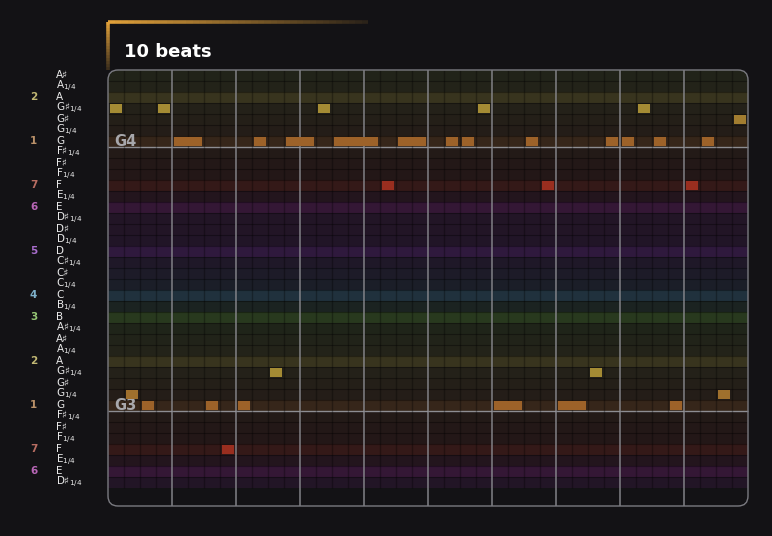
\includegraphics[width=\linewidth]{g_ciclo_aguda_mata.png}\caption{Voz aguda, ciclo A (10 pulsos).}
  \end{subfigure}\hfill
  \begin{subfigure}[b]{0.37\textwidth}\centering
    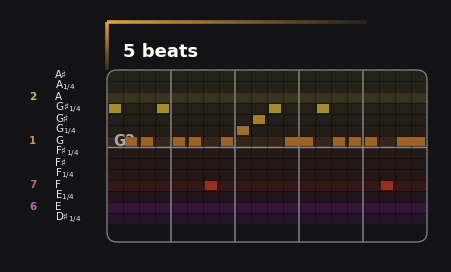
\includegraphics[width=\linewidth]{g_ciclo_grave_mata.png}\caption{Bajo, ciclo A (5 pulsos).}
  \end{subfigure}
  \caption{Patrones de ciclo de Mata Zyklek en 24-EDO. Cada fila es un grado y cada rectángulo, una nota que se repite en todas las vueltas. «Beats»: pulsos.}\label{fig:patron-ciclo}
\end{figure}

\begin{figure}[htbp]
  \centering
  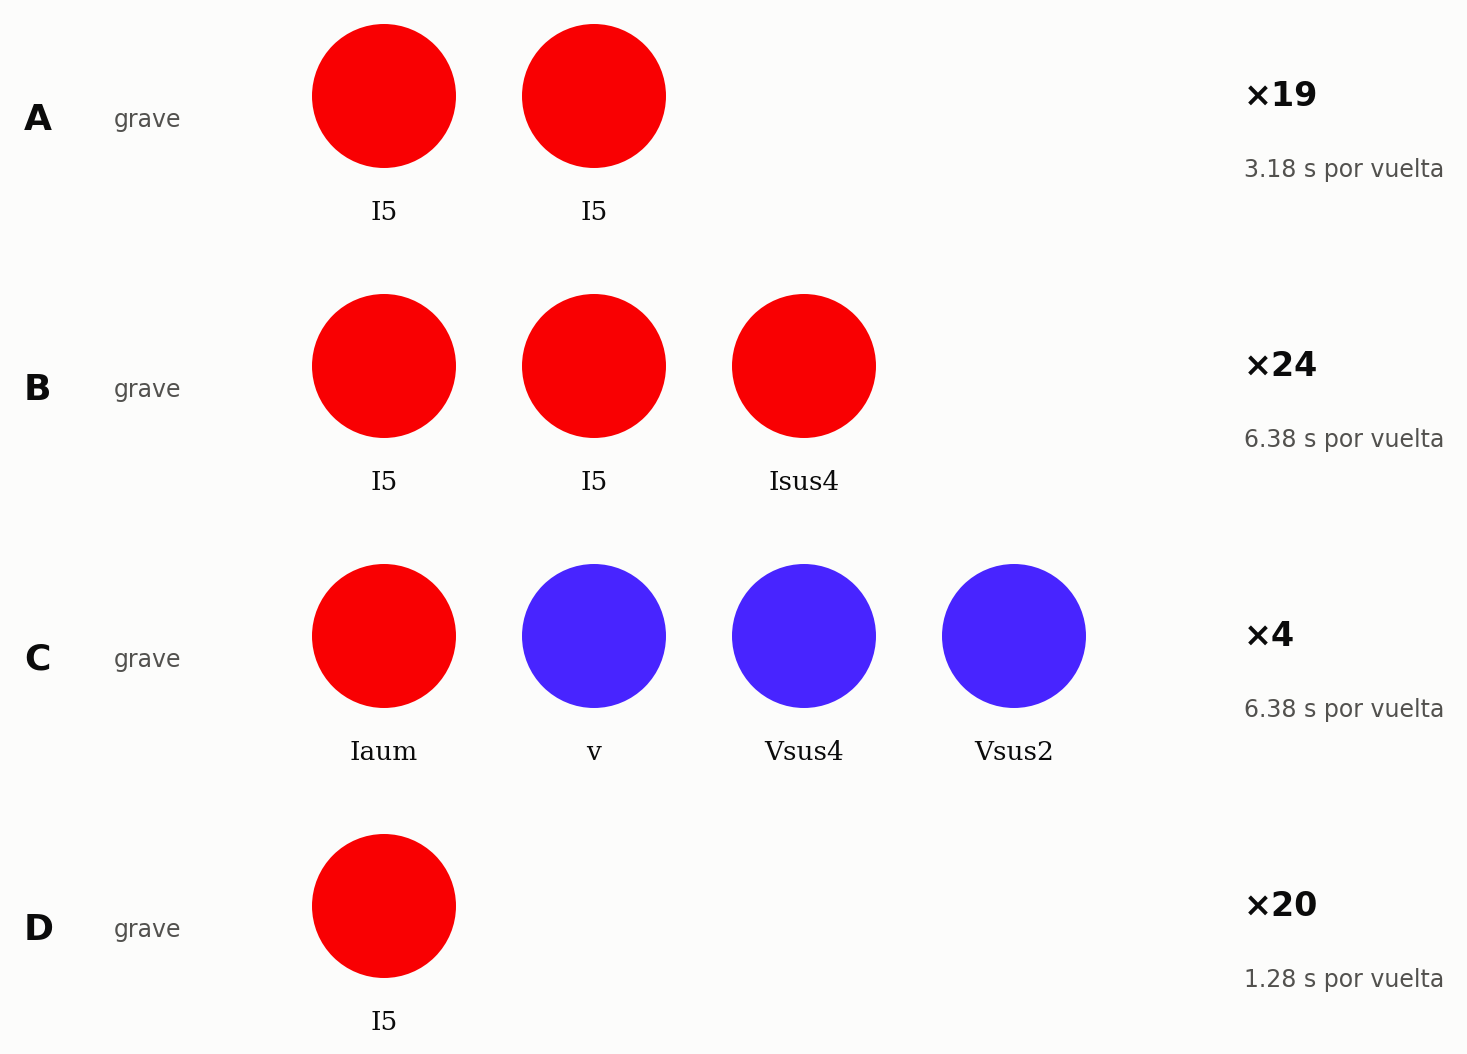
\includegraphics[width=0.75\textwidth]{mata_zyklek_tira_de_ciclos.png}
  \caption{Tira de ciclos de Mata Zyklek (centro Sol; modo \fl2+, 3, \fl6+, \fl7). Cada fila es un ciclo; cada círculo, la fundamental de un compás, con el color de su grado. A la derecha, número de vueltas ($\times$) y duración de cada vuelta.}\label{fig:tira-mata}
\end{figure}

\subsection{Consenso entre vueltas y atracción al registro}\label{sec:met-consenso}

Dentro de un ciclo de periodo $P \ge 2$~s, la saliencia de cada cuadro se reemplaza por su promedio con los cuadros
equivalentes de hasta tres vueltas antes y tres después:
\[
  \hat\Sigma(t, p) = \frac{1}{|K_t|} \sum_{k \in K_t} \Sigma(t + kP, p), \qquad
  K_t = \{k \in \{-3, \dots, 3\} : t + kP \text{ está en el ciclo}\},
\]
siempre que $|K_t| \ge 3$. Un error de una vuelta queda diluido entre las demás; una nota que se repite en todas las
vueltas se refuerza. Este es el paso que hace posible leer cuartos de tono: sin él, un cuarto de tono aislado no se
distingue de una nota desafinada.

Después se calcula un contorno de base con Viterbi sobre $\hat\Sigma$, se toma su mediana $r$ como el registro típico de la
melodía en la canción y se multiplica la saliencia por una atracción suave hacia ese registro:
\[
  w(p) = 0.7 + 0.3 \exp\!\Bigl(-\tfrac12 \bigl(\tfrac{p - r}{12}\bigr)^2\Bigr).
\]
La atracción nunca baja de 0.7, así que no impide salir del registro; solo desempata a favor de la zona donde suele estar
la melodía y en contra de los armónicos agudos o del bajo doblado.

\subsection{Contorno, notas y limpieza}

El contorno final es el camino de Viterbi sobre $w \hat\Sigma$ (proposición~\ref{prop:viterbi}). La celda
\texttt{extract\_notes} lo convierte en notas: cuantiza la altura a la rejilla de 50 cents, corrigiendo la desafinación
global de la grabación respecto de La 440 (\texttt{tuning\_offset}); aplica un filtro de mediana de tres cuadros; y corta
una nota nueva en cada ataque detectado y en cada cambio de altura. La altura de cada nota es la mediana del contorno en su
duración. Finalmente, \texttt{drop\_loose\_notes} quita las notas de menos de 80~ms que no reaparecen, con $\pm75$~ms de
tolerancia, a la misma altura una vuelta antes y una vuelta después.

\subsection{Tempo, pulso y compases}\label{sec:met-compases}

\paragraph{Tempo.} La celda \texttt{estimate\_tempo} calcula la autocorrelación $a(\ell)$ de la envolvente de ataques y,
para cada tempo candidato entre 60 y 200 BPM, con periodo $\ell(b)$, el puntaje
\[
  s(b) = \Bigl[a(\ell) + \tfrac12 a(2\ell) + \tfrac14 a(4\ell)\Bigr] \exp\!\Bigl(-\tfrac12 \bigl(\tfrac{\log_2(b/120)}{0.8}
  \bigr)^2\Bigr),
\]
que suma la evidencia del pulso y de sus múltiplos y prefiere suavemente los tempos cercanos a 120 BPM.

\paragraph{Pulso.} \texttt{track\_beats} aplica la programación dinámica de \citet{ellis2007} (sección~\ref{sec:senal}) con
rigidez $\alpha = 400$.

\paragraph{Evidencia de inicio de compás.} En cada pulso $i$ se combinan, estandarizados, el golpe grave, el golpe general
y el cambio de contenido armónico respecto del pulso anterior:
\[
  e_i = z\bigl(o^{\mathrm{grave}}_i\bigr) + 0.5\, z\bigl(o_i\bigr) + 0.8\, z\bigl(1 - \cos(h_{i-1}, h_i)\bigr),
\]
donde $h_i$ es el perfil de alturas del pulso. Además, \texttt{meter\_cue} mide, para cada longitud $L$, la correlación
$\rho_L(i)$ entre los ataques alrededor del pulso $i$ y los de $L$ pulsos después.

\paragraph{Segmentación.} \texttt{segment\_bars} elige la división en compases $L_1, L_2, \dots$, con cada $L_k$ entre 2 y
8 pulsos, que maximiza
\[
  \sum_k \Bigl[ e_{s_k} + \log \pi(L_k) + L_k\, \rho_{L_k}(s_k) \Bigr] - 0.8\, \#\{k : L_k \ne L_{k-1}\},
\]
donde $s_k$ es el pulso en que empieza el compás $k$ y $\pi$ es una distribución previa de longitudes (4: 0.45; 7: 0.15;
3: 0.12; 2, 6 y 8: 0.08; 5: 0.06). El último término penaliza cambiar de compás. Es un problema de Viterbi sobre los
estados «compás de longitud $L$ que termina en el pulso $j$», y se resuelve con la proposición~\ref{prop:viterbi}.

\subsection{Perfiles por compás y acorde}

\paragraph{Perfiles.} Para cada compás se calcula el tiempo que suena cada una de las 24 clases en el bajo, $P^b$, y en la
voz aguda, $P^m$ (sin las notas de menos de un cuarto de pulso). \texttt{fold\_bar\_profiles} los suma sobre todas las
vueltas del ciclo que contiene al compás y mide el \emph{acuerdo} entre vueltas como el coseno medio entre el perfil de
cada vuelta y el perfil sumado.

\paragraph{Acorde.} Con $b = P^b / \|P^b\|_1$ y $m = P^m / \|P^m\|_1$, la celda \texttt{chord24} forma el perfil combinado
$C = (b + 0.6\, m) / \|b + 0.6\, m\|_1$ y, para cada fundamental $r \in \mathbb{Z}_{24}$ y cada calidad $q$ con conjunto de
intervalos $I_q$ (tabla~\ref{tab:calidades}), el puntaje
\[
  S(r, q) = (1 + \lambda) \sum_{i \in I_q} C_{r+i} - \lambda + \beta\, b_r - \gamma \bigl(|I_q| - 2\bigr),
\]
con $\lambda = 0.5$, $\beta = 0.5$ y $\gamma = 0.02$. El primer término premia lo que cae dentro del acorde y, como
$\sum_i C_i = 1$, equivale a restar $\lambda$ veces lo que cae fuera; el segundo premia que el bajo esté en la
fundamental; el tercero penaliza levemente los acordes con más notas, para preferir la quinta sola cuando la tercera no
suena. Se elige el par $(r^*, q^*)$ de mayor puntaje. La probabilidad de la fundamental es un softmax con temperatura
$\tau = 0.05$ sobre los mejores puntajes de cada fundamental:
\[
  p(r^*) = \frac{\exp\bigl(\max_q S(r^*, q)/\tau\bigr)}{\sum_{r} \exp\bigl(\max_q S(r, q)/\tau\bigr)}.
\]

\begin{ejemplo}
Sea un compás con el bajo siempre en Mi ($b_{\mathrm{Mi}} = 1$) y la voz aguda repartida por igual entre Mi, Sol y Si. Con
Mi en la clase 8, Sol en la 14 y Si en la 22, se tiene $C = (b + 0.6\, m)/1.6$, es decir, $C_8 = (1 + 0.2)/1.6 = 0.75$ y
$C_{14} = C_{22} = 0.2/1.6 = 0.125$. Para la fundamental Mi y la calidad m ($I = \{0, 6, 14\}$, que sobre Mi da las clases
8, 14 y 22), $S = 1.5 \cdot 1 - 0.5 + 0.5 \cdot 1 - 0.02 = 1.48$. Para la calidad 5 ($I = \{0, 14\}$), el ajuste solo
cubre $0.875$ y $S = 1.5 \cdot 0.875 - 0.5 + 0.5 = 1.3125$. Gana Mi menor. Si la voz aguda tocara Sol+ (clase 15) en vez de
Sol, la tercera neutra ($I = \{0, 7, 14\}$) obtendría el puntaje 1.48 y el acorde se leería como Mi con tercera neutra.
\end{ejemplo}

\paragraph{Confianza.} La confianza del compás es
\[
  \kappa = p(r^*) \cdot a \cdot \text{cobertura},
\]
con $a$ el acuerdo medio entre vueltas del bajo y de la voz aguda (o 1 si la canción no tiene ciclos, y 0.6 si el compás
queda fuera de ellos en una canción que sí los tiene) y la cobertura, la fracción del compás con notas.

La figura~\ref{fig:tabroll-armonia} muestra el resultado en Sarniezz: cada columna es un compás con el acorde leído en
24-EDO debajo (grado, calidad y nombre), y el color de la franja inferior indica la confianza.

\begin{figure}[htbp]
  \centering
  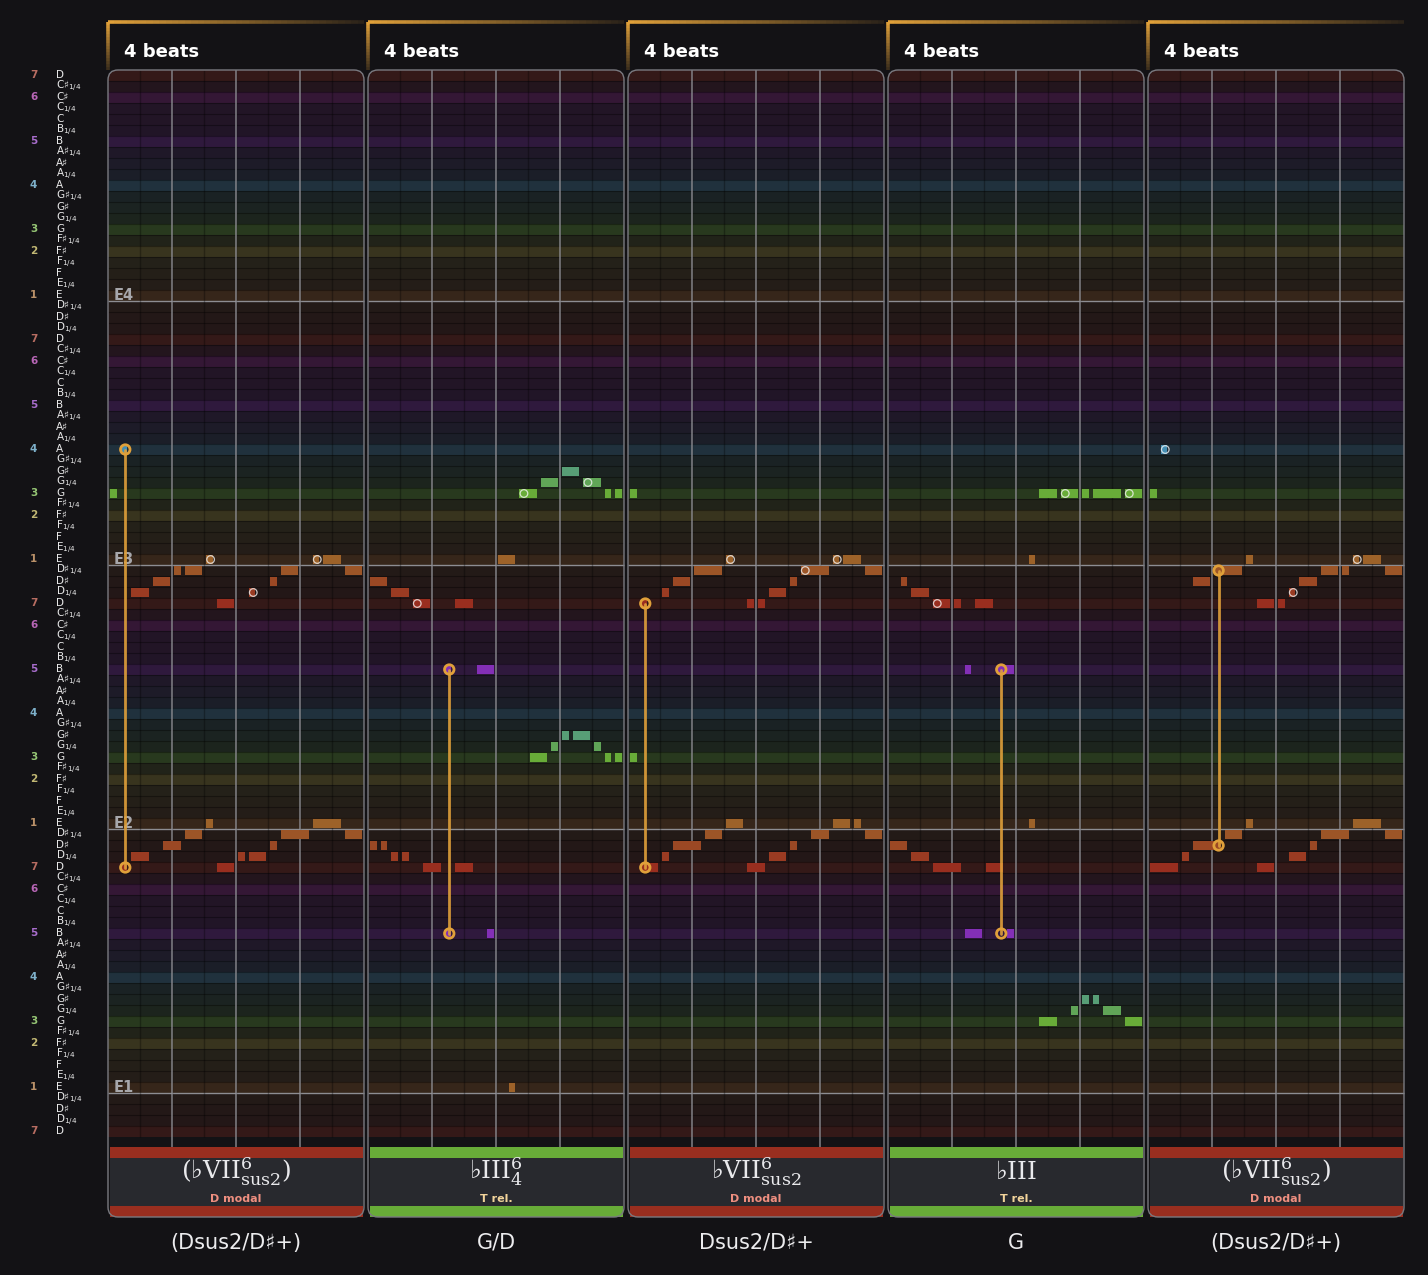
\includegraphics[width=0.85\textwidth]{g_tabroll_armonia_sarniezz.png}
  \caption{Tabroll con armonía (Sarniezz). Arriba, las notas en 24-EDO; debajo de cada compás, el acorde leído: grado, calidad, función y nombre. «Beats»: pulsos del compás.}\label{fig:tabroll-armonia}
\end{figure}

\subsection{Centro, modo y funciones}

\paragraph{Centro.} \texttt{center24\_by\_layer} calcula en cada capa tres repartos sobre las 24 clases: el tiempo que
suena cada clase ($T$), cuántas veces abre o cierra una vuelta del ciclo ($B$) y cuántas veces vuelve después de al menos
dos notas distintas ($R$). Cada reparto se normaliza a suma 1 y el puntaje de la capa es su promedio,
$\tfrac13 (T + B + R)$. El puntaje de la canción pesa el bajo el doble:
\[
  Z = \frac{2 Z^{\mathrm{bajo}} + Z^{\mathrm{aguda}}}{3}, \qquad
  \text{margen} = \frac{Z_{(1)} - Z_{(2)}}{Z_{(1)}},
\]
donde $Z_{(1)}$ y $Z_{(2)}$ son los dos mayores. Un margen menor que 0.1 marca un centro dudoso.

\paragraph{Modo.} \texttt{mode24} suma los perfiles de los compases confiables (bajo con peso 1 y voz aguda con 0.6),
los cuenta desde el centro y, para cada uno de los grados 2, 3, 6 y 7, elige entre su versión rebajada, neutra o natural
la que más suena.

\paragraph{Funciones y progresiones.} \texttt{chord\_roles} cifra cada acorde en números romanos y le asigna función,
eje e inversión (sección~\ref{sec:armonia-teoria}); \texttt{chord\_progressions} clasifica cada cambio de fundamental entre
compases confiables y cuenta las progresiones más frecuentes y los \emph{vaivenes}, idas y vueltas entre dos acordes.

\subsection{Columnas melódicas}

\texttt{melodic\_columns} elige, en cada pulso, la nota de la voz aguda más importante, a la manera de la reducción de
\citet{lerdahl1983}. Cada nota recibe el peso
\[
  \omega = 0.30\, \mu + 0.35\, \alpha + 0.20 \min\{1, d/\text{pulso}\} + 0.15\, \chi,
\]
donde $\mu$ es la posición métrica del ataque (primer pulso 1, mitad del compás 0.85, otro pulso 0.7, corchea 0.45, resto
0.3), $\alpha$ indica si la nota pertenece al acorde (1; a un cuarto de tono, 0.7; fuera, 0.2), $d$ es su duración y
$\chi$ si es un punto alto o bajo del contorno. La nota de más peso del compás, junto con el bajo que suena en ese
momento, es la \emph{columna principal}, que el tabroll marca con anillos dorados.

\section{Mejorar la melodía: hipótesis que se prueban}\label{sec:melodia-hipotesis}

Para mejorar la melodía se probaron varias ideas. Cada cambio se midió en las tres canciones con referencia y solo se
adoptaba si mejoraba en las tres (tabla~\ref{tab:hipotesis}).

\begin{table}[ht]
  \centering\small
  \caption{Ideas probadas para mejorar la melodía.}\label{tab:hipotesis}
  \begin{tabularx}{\textwidth}{@{}>{\raggedright}p{4.6cm}>{\raggedright}X l@{}}
    \toprule
    Idea & Qué pasó & Estado \\
    \midrule
    Consenso entre vueltas del looper & Más rápido y más estable & adoptada \\
    Atracción al registro de la melodía & Mata Zyklek pasa de 57 a 64 & adoptada \\
    Quitar notas sueltas & $+3$ puntos en las tres canciones & adoptada \\
    Guiarse por la partitura & La herramienta debe servir sin partitura; además no mejoraba de forma estable & descartada \\
    REPET (separar lo que se repite) & Solo deja en primer plano entre el 1 y el 18\,\% de la melodía & descartada \\
    Elegir la capa más nueva del looper & Funciona sobre la partitura, falla sobre el audio & descartada \\
    Estéreo por canal & La melodía sigue tapada en el 50--65\,\% de los cuadros & descartada \\
    Basic Pitch & Encuentra menos melodía y no da cuartos de tono & descartada \\
    Unir notas iguales seguidas & Borra re-ataques reales & descartada \\
    Votar la altura entre vueltas, refinar por armónicos, prueba de octava, otros umbrales & Ninguna mejora las tres
    canciones a la vez & descartadas \\
    Bajar el piso de la voz aguda & Empeora las tres canciones & descartada \\
    \bottomrule
  \end{tabularx}
\end{table}

\paragraph{Notas sueltas.} Por cada nota de la melodía principal, la herramienta detectaba 1.3 a 1.5 notas: unas eran de
otras capas del looper y la mayoría, pedazos cortos de una nota partida en cada ataque o cambio de altura. La regla
adoptada quita las notas de menos de 80~ms que no reaparecen a la misma altura una vuelta antes y una vuelta después;
entre esas notas solo el 6 a 24\,\% eran aciertos. La melodía principal pasó de 63.7 a 66.8 en Mata Zyklek, de 43.4 a
46.2 en Sarniezz y de 44.0 a 45.4 en Fabienk; el bajo, de 78.7 a 82.9, de 75.3 a 78.7 y de 63.8 a 69.3.

\paragraph{El looper y la melodía.} REPET \citep{rafii2013} aplicado a la vuelta del looper no sirve: la melodía se
repite en cada vuelta igual que el riff. Elegir la capa más nueva funcionaría con una transcripción perfecta, pero sobre
el audio la melodía aparece entre los picos de un cuadro suelto solo en el 32--43\,\% de los cuadros; la herramienta la
recupera mejor (44--68\,\%) porque promedia vueltas. La conclusión es que el looper ayuda a recuperar la melodía
promediando vueltas, no a separarla.

\paragraph{Basic Pitch.} Con el ajuste de notas cortas, Basic Pitch \citep{bittner2022} encuentra el 36, 47 y 48\,\% de
la melodía (Sarniezz, Mata Zyklek y Fabienk), menos que la herramienta (51, 69 y 49\,\%). Combinado con ella recupera
7--14 puntos más, pero esas notas caen sobre todo donde la herramienta ya tiene otra altura, y ninguna regla para
juntarlas mejora la medida principal. Su salida, en notas MIDI enteras, no sirve para cuartos de tono.

\section{Separar instrumentos}\label{sec:separacion}

La separación por defecto es Demucs \texttt{htdemucs\_6s} \citep{rouard2023}. Como alternativa se integró BS-RoFormer SW
\citep{lu2024}, que en las métricas públicas separa mejor la guitarra (SDR de 9.05 frente a 5.22~dB). El SDR
(\emph{signal-to-distortion ratio}) mide qué tan limpia sale una pista separada frente a la grabada por aparte. La
comparación se hizo sobre Sarniezz con la misma versión del cuaderno y los mismos ajustes; solo cambiaron las pistas. Para
que fuera reproducible se fijaron la versión de la herramienta de separación, el remuestreo, el solapamiento, la
precisión numérica, el número de hilos y la semilla, y se registró la huella SHA-256 del modelo. El resultado está en la
sección~\ref{sec:res-separacion}.

\section{La armonía por compás}\label{sec:armonia-metodo}

\paragraph{Entradas.} Para cada compás se usan el bajo y el contenido de la voz aguda en las 24 clases, sin contar las
notas de menos de un cuarto de pulso, que suelen ser de paso o adornos. El perfil de cada compás se suma sobre todas las
vueltas del ciclo que lo contiene, tomando el mismo punto del ciclo en cada vuelta; el bajo y la voz aguda usan sus
propios ciclos, porque pueden tener periodos distintos.

\paragraph{Acorde.} El perfil se compara con las ocho calidades de la tabla~\ref{tab:calidades}: cuenta lo que cae dentro
del acorde, resta lo que cae fuera y premia que el bajo esté en la fundamental, con peso 1 para el bajo y 0.6 para la voz
aguda.

\paragraph{Confianza.} La confianza $\kappa \in [0, 1]$ es el producto de tres factores: la probabilidad de la
fundamental elegida frente a las otras 23, el acuerdo entre las vueltas del ciclo en ese compás y la cobertura (qué parte
del compás tiene notas). Un compás es confiable si $\kappa \ge 0.5$. En canciones sin looper, como las de Primus, los
compases fuera de ciclo no se castigan.

\paragraph{Centro.} Se adapta la medida en tres partes de Piston para música sin dominante. En cada capa (bajo y voz
aguda) se suman, con el mismo peso, la nota que más tiempo suena, la que más aparece al principio y al final de cada vuelta
y la que más vuelve después de alejarse; el bajo pesa el doble. Elegir el centro solo por el bajo se descartó, porque en
Sarniezz y Fabienk el bajo descansa en \fl VII. El centro usado coincide con la tónica de oído en las cinco canciones
evaluadas (Mata Zyklek Sol, Sarniezz Mi, Fabienk Mi, Utzp Mi, Yor Zarad Sol).

\paragraph{Grado, función y progresión.} Cada acorde se cifra en números romanos sobre el centro, con «+» para el cuarto
de tono y «n» para la tercera neutra, y recibe su función (sección~\ref{sec:armonia-teoria}) y su eje de Lendvai. Cada
cambio de fundamental entre compases confiables se clasifica según el movimiento de la fundamental en la tabla de Piston
(quinta abajo, quinta arriba, tercera, segunda, tritono o microtonal) y según el eje (adelante, atrás, dentro del mismo
eje, en el mismo eje neutro o microtonal).

\section{Evaluación}\label{sec:evaluacion}

\paragraph{Medidas.} Se usa la medida F de notas, con el ataque a $\pm75$~ms y la altura en la misma casilla de 24-EDO.
Se mide para tres referencias: la \emph{melodía principal} de cada sección, elegida por el autor por criterio musical
(la voz que uno cantaría) y nunca mirando qué guitarra sigue la herramienta; la \emph{nota más aguda} de todas las
guitarras, más exigente; y el \emph{bajo}. Las versiones «sin octava» aceptan la misma clase en cualquier octava. Para la
armonía se mide la fundamental por compás, ponderada por su duración, en todos los compases y en los confiables.

\paragraph{Alineación.} El camino entre la partitura y el audio se obtiene por alineamiento temporal dinámico (DTW) y se
ajusta a una recta por sección, porque con looper el tempo no cambia dentro de una sección. Las ventanas incompatibles con
un tempo constante quedan fuera. Este criterio usa solo la alineación, nunca la salida de la herramienta. Se mide el 83\,\%
del tiempo de Mata Zyklek, el 83\,\% de Sarniezz y el 72\,\% de Fabienk.

\paragraph{Arbitraje a ciegas.} Donde la herramienta y la partitura corregida dan alturas distintas una y otra vez, el
autor juzgó de oído, sin saber cuál era cuál. Cada clip tiene la pista de guitarra real en un canal y la partitura
sintetizada en el otro, en tres versiones en orden al azar: la nota escrita, un cuarto de tono arriba y un cuarto de tono
abajo. La regla se fijó antes de escuchar: una nota cambia si al menos dos clips eligen la misma altura distinta de la
partitura, con seguridad media o alta. En la primera ronda (21 clips, 3 de ellos controles, todos correctos) la partitura
tenía razón en la mitad de los casos decididos: un desacuerdo no basta para corregirla, porque la herramienta también se
equivoca en cuartos de tono. La segunda ronda (21 clips) corrigió tres notas de Sarniezz, una pista de Fabienk y añadió
una nota de Mata Zyklek.

\paragraph{Prueba ciega.} Yor Zarad se reservó sin abrir ninguna salida de la herramienta, y su referencia se armó a
ciegas (sección~\ref{sec:referencias}). La medida se hizo una sola vez, sobre la corrida congelada.

\paragraph{Reproducibilidad.} Con las mismas pistas, la herramienta da el mismo resultado: entre 8 y 12 corridas por
canción dieron las mismas notas, la misma F y la misma tabla por compás. Demucs era el único paso al azar (desplaza el
audio entre 0 y 0.5~s antes de separar): con el mismo código, Mata Zyklek dio 57.2 con unas pistas y 61.6 con otras.
Desde entonces la semilla queda fija, y cada corrida guarda la huella SHA-256 \citep{nist2015} de la mezcla y de las dos
pistas, de modo que dos corridas con las mismas huellas usaron exactamente el mismo audio. Un hallazgo solo cuenta si se
mantiene con las dos separaciones. Ninguna celda del cuaderno lee la partitura ni nombra una canción.

\section{Comparación con estilos}\label{sec:comparacion}

\subsection{Matriz de verosimilitud armónica}

Cada estilo se resume por el centro de su corpus en dos cosas: qué fundamentales suenan y cuánto tiempo (12 grados
respecto de la tónica) y cómo se cambia de fundamental (intervalo del cambio y grado de llegada, $12 \times 12$). La
verosimilitud de una canción en un estilo es el percentil de tipicidad respecto del centro, promediado entre esas dos
partes; con menos de tres cambios de acorde, solo cuenta la de las fundamentales. Las fundamentales de la canción se
toman de los compases confiables.

La figura~\ref{fig:matriz-rock-pop} muestra la forma del resultado con los dos estilos más cercanos, rock y pop. Cada
celda es un percentil: 50 es una pieza típica del estilo y 0, una más rara que todas las del corpus.

\begin{figure}[htbp]
  \centering
  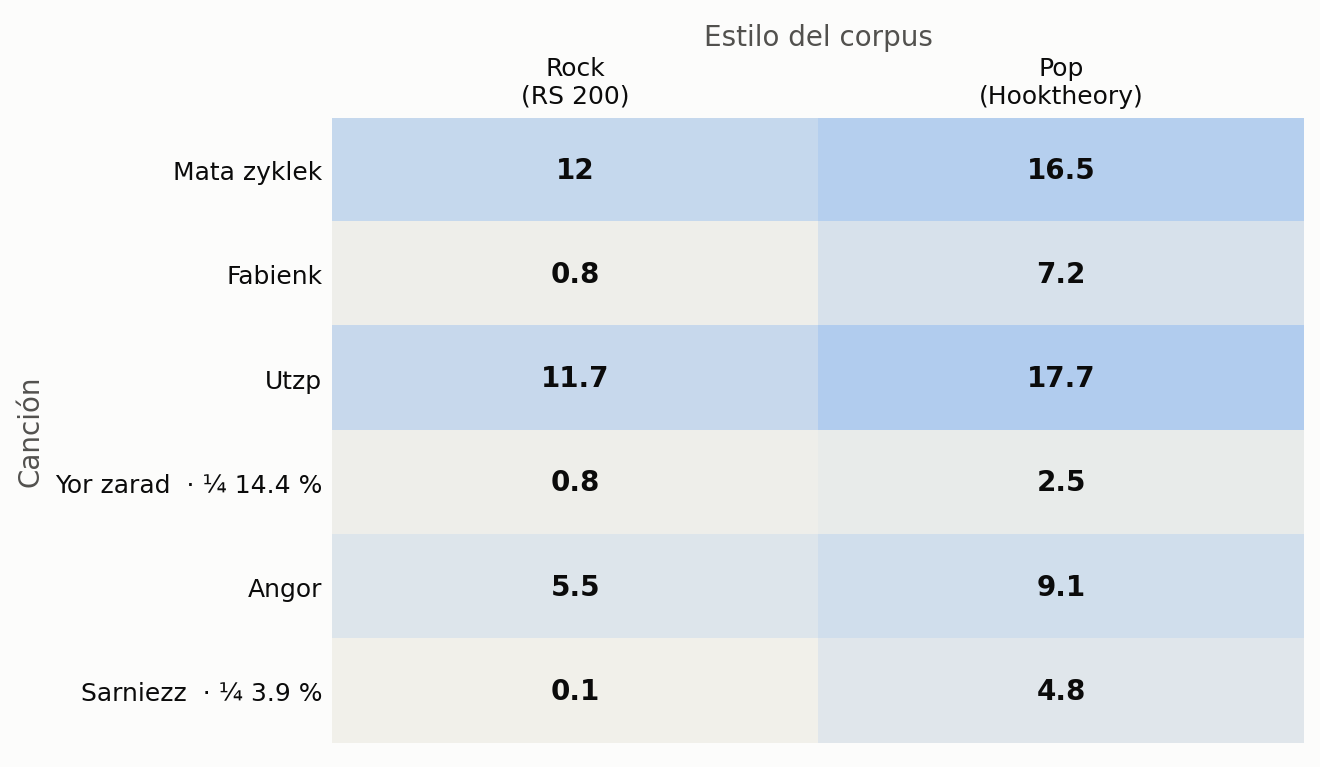
\includegraphics[width=0.6\textwidth]{g_matriz_rock_pop.png}
  \caption{Matriz de verosimilitud frente a rock (RS~200) y pop (Hooktheory). Cada celda es un percentil: 50 = típica del estilo; 0 = más rara que todo el corpus. Junto al nombre, el tiempo con la fundamental en cuarto de tono.}\label{fig:matriz-rock-pop}
\end{figure}

\subsection{Test por bloques}

Cada canción se resume en cuatro bloques de rasgos, y cada bloque se compara con cada corpus que lo tenga:
\begin{itemize}
  \item \textbf{Armonía:} fundamentales y cambios de fundamental, como en la matriz.
  \item \textbf{Escala (12 notas):} la melodía en 12 grados respecto de la tónica, por duración; cada cuarto de tono se
  reparte mitad y mitad entre sus dos vecinos.
  \item \textbf{Cuartos de tono:} el reparto del tiempo entre los 12 grados en cuarto de tono, comparado solo con los
  corpus microtonales.
  \item \textbf{Metro:} el reparto del tiempo por familia de compás (2·4·8, 3·6·12, 5, 7, 9 u otro impar).
\end{itemize}

La tipicidad de un bloque se mide con el percentil por vecinos ($k = 5$). Una canción solo pasa al bloque de cuartos de
tono si la concentración de sus cuartos de tono (sección~\ref{sec:metodo-cuartos}) supera a la de los controles por al
menos dos desviaciones estándar; si no, se trata como una canción de 12 notas.

\paragraph{Modelo de medición.} La herramienta marca entre 9 y 13\,\% de cuartos de tono en música que no los tiene y lee
mal algunos compases de un 4/4. Para comparar en igualdad, cada pieza de corpus pasa por el mismo error: en la altura, una
fracción $\varepsilon$ del tiempo de cada grado se reparte entre sus dos vecinos a un cuarto de tono; en el metro, una
fracción $\eta$ pasa a las familias de compás en que la herramienta se equivoca. Ambas se miden en los controles de
Primus ($\varepsilon = 0.113$).

\paragraph{Veredicto.} Con un umbral $u = 5$\,\%, como un contraste a una cola:
\begin{itemize}
  \item \emph{estilo existente (X)}: algún corpus X con todos los bloques medidos tiene percentil conjunto $\ge u$;
  \item \emph{variante atípica de X}: cada bloque es típico en X por separado, pero la combinación no lo es;
  \item \emph{síntesis de lenguajes existentes}: cada bloque es típico en algún corpus, pero ningún corpus explica la
  combinación;
  \item \emph{rasgo sin vecino}: algún bloque no es típico en ningún corpus.
\end{itemize}
El percentil conjunto mide el parecido en todos los bloques a la vez, con la suma de las distancias de cada bloque
divididas por su mediana en el corpus. Solo cuentan los corpus con 100 piezas o más.

\paragraph{Calibración.} El mismo veredicto se aplica a cada pieza de los corpus con al menos tres bloques, contra las
demás, para saber cuántas veces el método llama «síntesis» o «sin vecino» a una pieza real de un estilo conocido.

\section{Cuartos de tono: adorno o grado}\label{sec:metodo-cuartos}

Cada nota en cuarto de tono de la voz aguda se clasifica como \emph{inflexión} (adorno) si dura menos que la nota mediana
de la canción y llega o sale por un paso de cuarto de tono hacia un grado regular (un bend, un slide, una nota de paso), y
como \emph{grado} en cualquier otro caso. La \emph{concentración} es el porcentaje del tiempo en cuartos de tono que cae
en los dos grados más usados: si es alta, los cuartos de tono son grados elegidos de la escala; si se reparten por igual
entre muchos grados, son desafinación o adorno. Para cada grado en cuarto de tono se mide además en qué porcentaje de las
vueltas del ciclo principal aparece.

El \emph{piso de ruido} se mide en Primus: la herramienta marca allí entre el 9 y el 13\,\% de la melodía en cuartos de
tono, casi todo como inflexión. La proporción de tiempo en cuartos de tono no sirve para separar a la banda (Utzp marca
11\,\%), pero la concentración sí: en Primus está entre 28 y 37\,\%.

\section{Ciclos métricos}

La herramienta parte la canción en compases de 2 a 8 pulsos, así que un ciclo más largo sale partido en trozos (por
ejemplo $4 + 4 + 4 + 7$). Para encontrar los ciclos largos se calcula $R(\ell)$ en una rejilla de corcheas, para $\ell$
de 2 a 40, en toda la canción y en ventanas de 30~s. Además se listan los tramos seguidos de compases con el mismo número
de pulsos y se buscan patrones de compases que se repiten.

\section{Implementación}

El cuaderno de Jupyter es la fuente de verdad del análisis. Un script lo divide en un módulo por celda y guarda la huella
de cada uno; si un módulo se edita a mano, la extracción se detiene en lugar de borrar el cambio. Otro script corre todas
las celdas sobre una canción, de punta a punta, y guarda el tabroll, la armonía, los ciclos y un resumen con las huellas
del audio usado. El repositorio incluye las referencias, la documentación, las pruebas automáticas y la presentación. Está
escrito en Python con \texttt{librosa} \citep{mcfee2015}. El código es público en
\url{https://github.com/NewForest2005/analisis-computacional-tabroll}.

\chapter{La herramienta}\label{cap:herramienta}

Este capítulo describe cómo está construida la herramienta y qué garantiza que sus resultados se puedan reproducir.
Interesa por dos razones: un análisis computacional solo es verificable si otra persona puede correrlo y obtener lo
mismo, y varias decisiones de diseño (la semilla, las huellas, la prohibición de leer la partitura) son condiciones para
que la evaluación del capítulo~\ref{cap:resultados} sea honesta.

\section{Del cuaderno al repositorio}

El análisis vive en un cuaderno de Jupyter, que es la \emph{fuente de verdad}: todo cambio se hace en él. El cuaderno
empezó en Google Colab y pasó a un repositorio de GitHub cuando la memoria disponible dejó de alcanzar. Para poder probar
y reutilizar cada paso por separado, un script lo divide en módulos de Python, uno por celda: 123 módulos en
\texttt{src/tabroll/cells/}. Al extraerlos guarda la huella SHA-256 de cada módulo; si alguien edita uno a mano, la
siguiente extracción lo detecta y se detiene, en lugar de borrar el cambio. Una prueba automática falla si el cuaderno y
los módulos no coinciden. Así el cuaderno siempre manda.

\section{Una corrida}

Un script corre todas las celdas del cuaderno sobre una canción, de punta a punta, sin abrir Jupyter, y guarda todo en una
carpeta con la fecha, la hora y el nombre de la canción (tabla~\ref{tab:salidas}). Si las pistas de guitarra y bajo no
existen junto al audio, Demucs las crea. Los ajustes que se pasen en la línea de comandos solo afectan esa corrida; el
cuaderno no se modifica.

\begin{table}[ht]
  \centering\small
  \caption{Lo que guarda cada corrida.}\label{tab:salidas}
  \begin{tabularx}{\textwidth}{@{}l>{\raggedright\arraybackslash}X@{}}
    \toprule
    Archivo & Contenido \\
    \midrule
    Imágenes & Tabroll por páginas e imagen completa, tabroll con la armonía en 24-EDO, mapa de ciclos y círculo armónico \\
    Resumen & Tempo, tonalidad, compases, ciclos, capas del looper y huellas SHA-256 del audio usado \\
    Salida & Todo lo que imprime el cuaderno, con el tiempo de cada celda \\
    Armonía & Una fila por compás (fundamental, calidad, grado, bajo, confianza, ciclos, perfiles) y el resumen de la canción \\
    Diagnóstico de la línea & Las notas de la voz aguda y del bajo, la saliencia y los ciclos, para la evaluación \\
    Evaluación & Solo en las canciones con referencia: medidas globales y por sección, y la armonía por compás \\
    \bottomrule
  \end{tabularx}
\end{table}

\paragraph{La evaluación está separada del análisis.} El módulo de evaluación compara la salida con la referencia
\emph{después} de la corrida. Ninguna celda del cuaderno lee la partitura ni nombra una canción, salvo la que elige el
audio; una prueba automática lo verifica. Esto impide que la herramienta se ajuste, sin querer, a las canciones con las que
se mide.

\section{Reproducibilidad}

\paragraph{Corridas congeladas.} Las cifras de acierto del trabajo vienen de corridas congeladas del 13 de noviembre de
2026, marcadas con un sufijo propio, que no se vuelven a ejecutar. Las mismas pistas dan las mismas notas: entre 8 y 12
corridas de cada canción, con distintas versiones del cuaderno, dieron la misma medida F y la misma tabla por compás.

\paragraph{Semilla y huellas.} Demucs desplaza el audio entre 0 y 0.5~s antes de separar, al azar, y eso cambiaba el
resultado (57.2 frente a 61.6 en Mata Zyklek). La semilla quedó fija en 0, y cada corrida guarda la huella de la mezcla y de
las dos pistas. Dos corridas con las mismas huellas usaron exactamente el mismo audio.

\paragraph{El separador alternativo.} Para BS-RoFormer, que no publica autor ni licencia de sus pesos, se fijó todo lo que
puede cambiar el resultado (tabla~\ref{tab:roformer}). Dos separaciones del mismo fragmento salieron idénticas bit a bit.

\begin{table}[ht]
  \centering\small
  \caption{Parámetros fijados para BS-RoFormer SW.}\label{tab:roformer}
  \begin{tabularx}{\textwidth}{@{}l l >{\raggedright\arraybackslash}X@{}}
    \toprule
    Parámetro & Valor & Por qué \\
    \midrule
    Herramienta de separación & audio-separator 0.48.0 & el solapamiento por defecto cambió en la 0.47.0 \\
    Entrada & 44.1 kHz estéreo, 32 bits flotantes & el remuestreo no depende de la herramienta \\
    Solapamiento & 2 & el de las métricas públicas \\
    Precisión / dispositivo & 32 bits / CPU & sin precisión mixta \\
    Hilos & 8, fijos & el número de hilos puede alterar el orden de las sumas \\
    Semilla & 0, con algoritmos deterministas & \\
    Salida & FLAC & el MP3 añade artefactos en los parciales que se transcriben \\
    Modelo & huella SHA-256 \texttt{24e7d35e\dots} & los pesos no tienen versión oficial \\
    \bottomrule
  \end{tabularx}
\end{table}

\section{Pruebas y gráficas}

El repositorio tiene 99 funciones de prueba en 23 archivos. Cubren la extracción de celdas y su protección, la lectura de
las partituras de Guitar Pro y su alineación con el audio, la evaluación de la melodía, la armonía en 24-EDO, el centro,
las funciones, las columnas melódicas, los patrones de ciclo, la limpieza de notas, la reproducibilidad y las gráficas.

Las gráficas también se prueban. Un módulo común arma cada figura en tres franjas (encabezado, cuerpo y pie) y una función
de revisión dibuja la figura y detecta textos que se salen, textos que se montan, leyendas sobre los datos y franjas
vacías. Una prueba arma las figuras principales con datos sintéticos del tamaño real (36 canciones, nombres largos) y exige
que la revisión no encuentre problemas.

\section{Costo}

En un computador portátil con procesador Intel de 8 núcleos y 16~GB de memoria, sin GPU:
\begin{itemize}
  \item Demucs separa una canción en varios minutos.
  \item El cuaderno completo tarda unos 3 minutos por canción (183.6~s en Sarniezz). Calcular una sola vez lo que comparten
  las dos saliencias de la voz aguda redujo ese paso de 78 a 40~s en Mata Zyklek, con resultados idénticos.
  \item BS-RoFormer tardó 3\,616~s en Sarniezz: 13.1 veces la duración de la canción.
  \item Las gráficas de la comparación con estilos tardan unos 5 a 6 minutos.
\end{itemize}

\chapter{Resultados}\label{cap:resultados}

Todas las cifras de acierto de este capítulo vienen de las corridas congeladas del 13 de noviembre de 2026, con las
pistas de Demucs de semilla 0. Las gráficas de la comparación con estilos usan la corrida más reciente de cada canción.

\section{Qué detecta la herramienta}\label{sec:res-acierto}

La tabla~\ref{tab:acierto} y la figura~\ref{fig:acierto} comparan la salida de la herramienta con las referencias
corregidas de oído. En promedio, la melodía principal acierta el 49\,\% y la fundamental del acorde, el 85\,\% en los
compases confiables.

\begin{figure}[htbp]
  \centering
  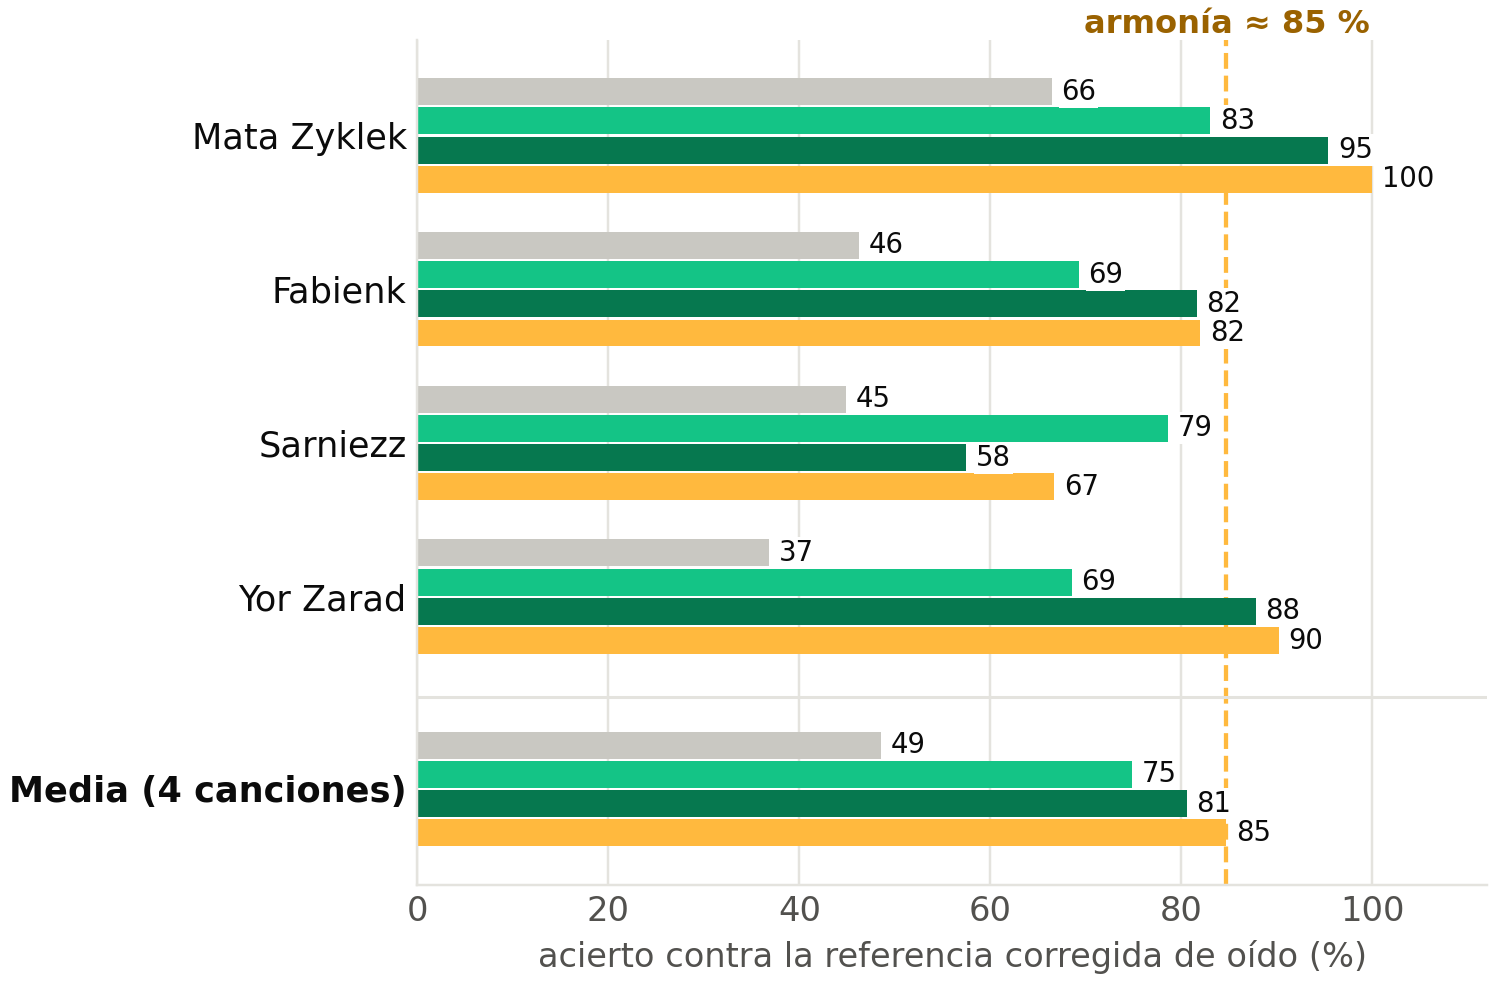
\includegraphics[width=0.72\textwidth]{acierto_herramienta.png}
  \caption{Acierto de la herramienta por canción, contra la referencia corregida de oído. Gris: melodía principal; verde claro: bajo; verde oscuro: fundamental del acorde; amarillo: fundamental en compases confiables, cuya media (línea punteada) es del 85\,\%.}\label{fig:acierto}
\end{figure}

\begin{table}[ht]
  \centering
  \caption{Acierto contra las referencias corregidas de oído (medida F para melodía y bajo; \% del tiempo para la
  fundamental).}\label{tab:acierto}
  \begin{tabular}{@{}lrrrr@{}}
    \toprule
    Canción & Melodía principal & Bajo & Fundamental & Fundamental (confiables) \\
    \midrule
    Mata Zyklek & 66.4 & 83.0 & 95.4 & 100 \\
    Fabienk & 46.2 & 69.2 & 81.6 & 82 \\
    Sarniezz & 44.9 & 78.6 & 57.5 & 67 \\
    Yor Zarad (a ciegas) & 36.8 & 68.6 & 87.8 & 90.2 \\
    \midrule
    \textbf{Media} & \textbf{49} & \textbf{75} & \textbf{81} & \textbf{85} \\
    \bottomrule
  \end{tabular}
\end{table}

\subsection{Por qué la armonía es fiable aunque la melodía no lo sea tanto}

La diferencia entre la melodía y la armonía no es casual. Cuatro rasgos del método la explican:
\begin{enumerate}
  \item \textbf{El bajo manda.} Al decidir la fundamental pesa más el bajo (1 frente a 0.6), que es la voz mejor
  transcrita.
  \item \textbf{Se suma sobre las vueltas del loop.} Un error en una vuelta queda en minoría frente a las demás.
  \item \textbf{La octava no importa.} Una nota una octava arriba es la misma clase de altura. La mayoría de los errores
  de la melodía son la nota correcta en otra octava, o una nota correcta de otro loop de guitarra.
  \item \textbf{Por compás, no por nota.} La melodía exige acertar el ataque a $\pm75$~ms; el acorde solo pide saber qué
  notas suenan en el compás.
\end{enumerate}

Un experimento aparte lo confirma: al cambiar solo el peso de la melodía (tres valores), su acierto varió (Fabienk de
40.8 a 44.2, Sarniezz de 46.0 a 47.9), pero la fundamental quedó idéntica en las tres corridas (82.3 y 72.3). Esas
corridas son de una versión anterior del cuaderno, así que lo que se cita es la invariancia, no los valores absolutos.

\subsection{La prueba ciega}

En Yor Zarad, medida una sola vez sobre la corrida congelada, la melodía principal acierta 36.8 (47.7 sin contar la
octava) y el bajo, 68.6. La armonía sale entre las mejores del álbum: fundamental 87.8\,\% en 99 compases (90.2\,\% en los
confiables), fundamental y calidad 43.0\,\%, bajo 94.2\,\% y el mismo centro (Sol) que la partitura. El fallo principal es
que el riff grave sale una octava arriba, porque la voz aguda nunca baja de Si2; el autor confirmó a ciegas que la
referencia tenía razón.

\subsection{La armonía frente a referencias más completas}

Sumar a la referencia corregida todas las guitarras de Guitar Pro cambia la fundamental en pocos compases (0, 7 y 3\,\%) y
sube el acierto de la herramienta entre 0 y 1.3 puntos (tabla~\ref{tab:ref-completa}): la referencia corregida era
representativa. La partitura de Guitar Pro sola solo es fiable en Mata Zyklek.

\begin{table}[ht]
  \centering
  \caption{Fundamental correcta (\%) según la referencia.}\label{tab:ref-completa}
  \begin{tabular}{@{}lrrr@{}}
    \toprule
    Canción & Corregida & Completa & Guitar Pro sola \\
    \midrule
    Mata Zyklek & 95.4 & 95.4 & 93.8 \\
    Sarniezz & 57.5 & 58.6 & 37.8 \\
    Fabienk & 81.6 & 82.9 & 58.8 \\
    \bottomrule
  \end{tabular}
\end{table}

La función armónica coincide con la de la partitura casi lo mismo que la fundamental (66.0\,\% en Sarniezz, 98.1\,\% en Mata
Zyklek y 82.9\,\% en Fabienk; 90.4, 98.8 y 83.5\,\% en los compases confiables): los errores vienen de la fundamental, no
del etiquetado. Sarniezz es el punto débil: uno de sus acordes más frecuentes, \fl VIIsus2, comparte notas con sus vecinos, y su bajo de
Mi suena un cuarto de tono bajo y la herramienta lo lee como Re\sh+.

\section{Separación: un resultado negativo}\label{sec:res-separacion}

BS-RoFormer separa la guitarra mucho mejor que Demucs según las métricas públicas, pero la melodía de Sarniezz quedó igual
con los dos (tabla~\ref{tab:separacion}). Además, BS-RoFormer tardó 3\,616~s (unos 60 minutos, 13 veces la duración de la
canción) en separarla en CPU.

\begin{table}[ht]
  \centering
  \caption{Demucs frente a BS-RoFormer SW en Sarniezz (\% de acierto contra la partitura corregida).}\label{tab:separacion}
  \begin{tabular}{@{}lrr@{}}
    \toprule
    & Demucs & BS-RoFormer SW \\
    \midrule
    SDR de guitarra (métrica pública, dB) & 5.22 & 9.05 \\
    Melodía principal & 44.9 & 44.9 \\
    Melodía principal, sin octava & 51.1 & 51.8 \\
    Nota más aguda & 35.3 & 30.9 \\
    Bajo & 78.6 & 76.5 \\
    \bottomrule
  \end{tabular}
\end{table}

Por sección, BS-RoFormer ayuda donde suenan dos guitarras con una frase aguda (c.~43--51: de 19.3 a 43.0) y empeora donde
la guitarra toca sola sobre el bajo (c.~27--30: de 55.9 a 40.3). La dificultad está dentro de la guitarra: el looper
superpone varias capas del mismo instrumento y ningún separador las distingue. El resultado no invalida el trabajo:
muestra que la medida no depende del separador y ubica con precisión el cuello de botella, que es separar las capas del
looper, no medir los cuartos de tono. Demucs se mantiene como separador por defecto.

\section{Armonía: fuera de todos los corpus}\label{sec:res-armonia}

Frente a los cuatro corpus de armonía, los estilos más cercanos son el rock y el pop, pero ninguna canción pasa de 17.7
(Utzp en pop), cuando una pieza típica daría 50 (figura~\ref{fig:matriz}). Las canciones con pedal (Mata Zyklek y Utzp)
quedan cerca del borde del rock (12 y 11.7); Fabienk, Sarniezz y Yor Zarad quedan por debajo de 1 en rock. La práctica
común y el jazz no encajan con ninguna canción. La matriz con las 36 canciones medidas, incluidos los repertorios, está en
el apéndice (figura~\ref{fig:g-matriz}).

\begin{figure}[htbp]
  \centering
  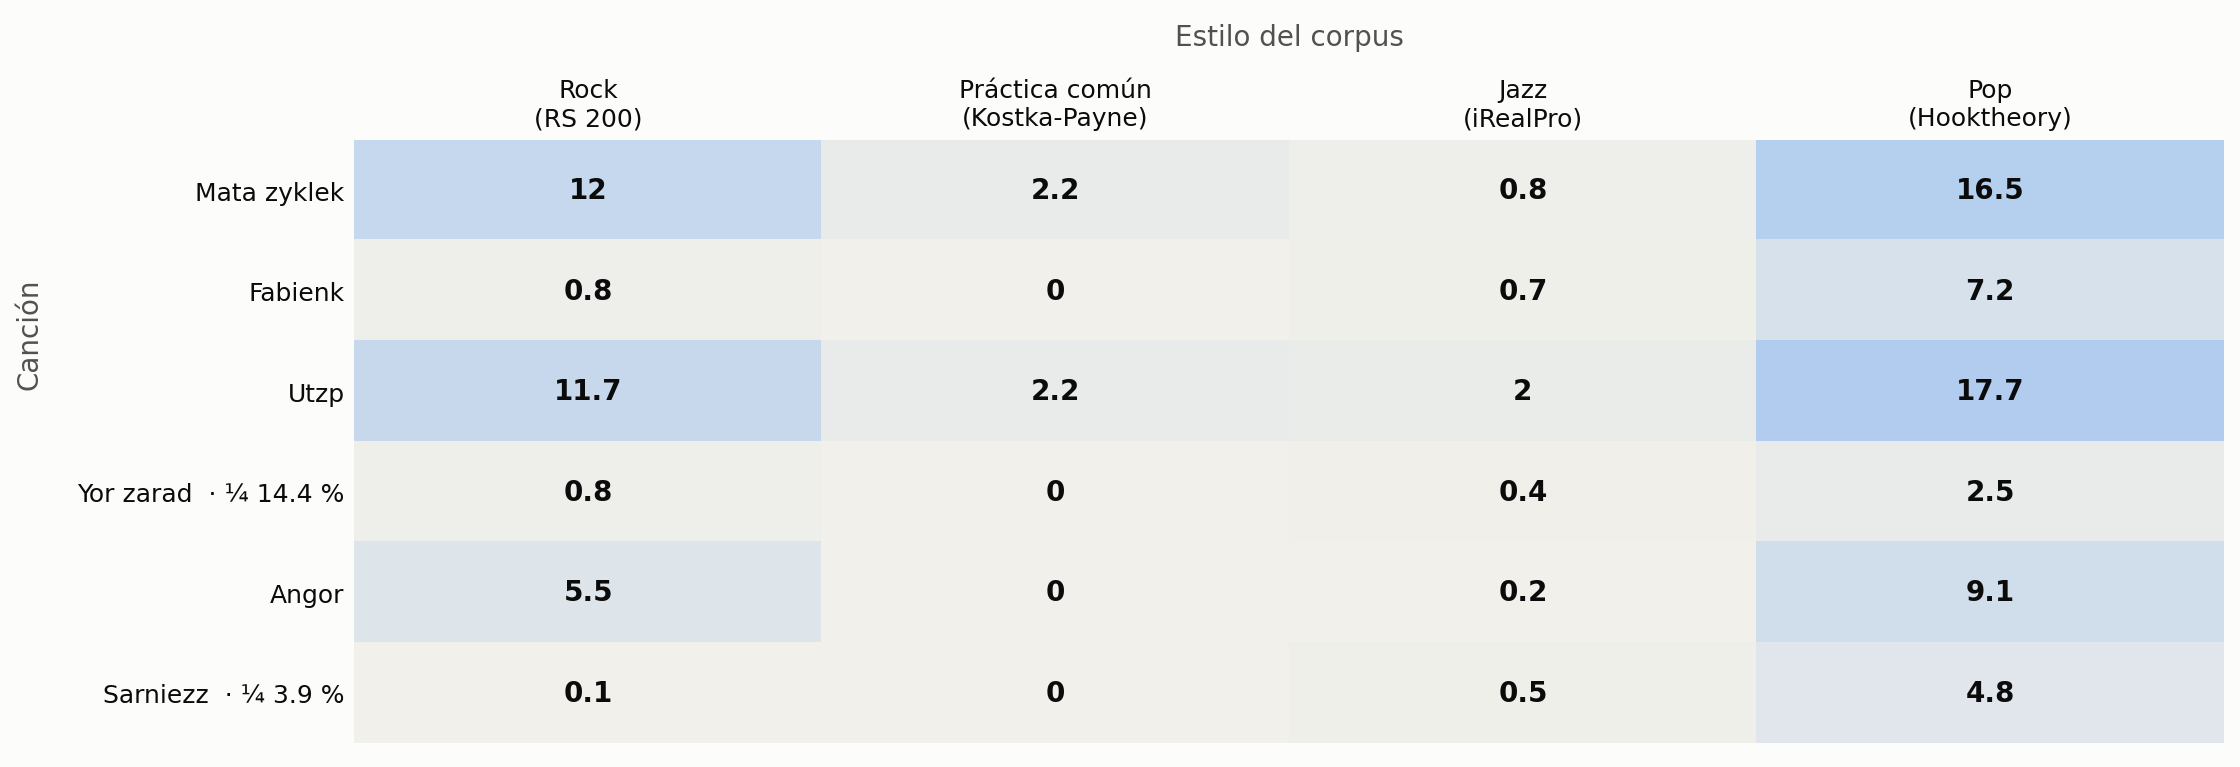
\includegraphics[width=\textwidth]{1a_armonia_matriz_verosimilitud.png}
  \caption{Matriz de verosimilitud armónica del álbum frente a rock (RS~200), práctica común (Kostka-Payne), jazz (iRealPro) y pop (Hooktheory). Percentil: 50 = típica; 0 = más rara que todas. «¼\,\%»: tiempo con fundamental en cuarto de tono.}
  \label{fig:matriz}
\end{figure}

El método no exagera la novedad. Calibrado con 388 piezas reales de rock, comparadas contra las demás, da «estilo
existente» el 92.3\,\% de las veces y «sin vecino» solo el 5.2\,\%. En la banda, el 37.5\,\% de los casos (9 de los 24
bloques de las seis canciones) queda sin vecino.

El mapa de la figura~\ref{fig:mapa} lo muestra de otra forma. Cada canción y cada pieza de corpus se reduce a su reparto
de fundamentales en 12 grados desde su tónica, de modo que la tonalidad no importa, y el análisis de componentes
principales comprime esos doce números en las dos direcciones en que más se diferencian las piezas. El eje horizontal
crece con el peso de II y VI y decrece con el de la tónica; el vertical baja cuando pesan \fl VI, \fl VII y \fl III. Dos
puntos cercanos tienen repartos parecidos. Mata Zyklek y Utzp, que se apoyan en un pedal sobre la tónica, quedan en el
borde del rock; Sarniezz y Fabienk caen donde no hay piezas de ningún corpus, por el peso de \fl VII y \fl III (en
Sarniezz, \fl III ocupa el 42\,\% del tiempo). El mismo mapa con los repertorios de King Gizzard, Zappa, King Crimson y Gentle Giant está en el apéndice
(figura~\ref{fig:g-mapa}). Las estrellas son, de arriba abajo: Mata Zyklek $(-0.48,\ 0.03)$, Angor
$(-0.52,\ -0.05)$, Utzp $(-0.51,\ -0.10)$, Yor Zarad $(-0.46,\ -0.17)$, Fabienk $(-0.21,\ -0.55)$ y Sarniezz
$(-0.21,\ -0.63)$. Angor cae en el mismo punto que «Flying Microtonal Banana» de King Gizzard.

\begin{figure}[htbp]
  \centering
  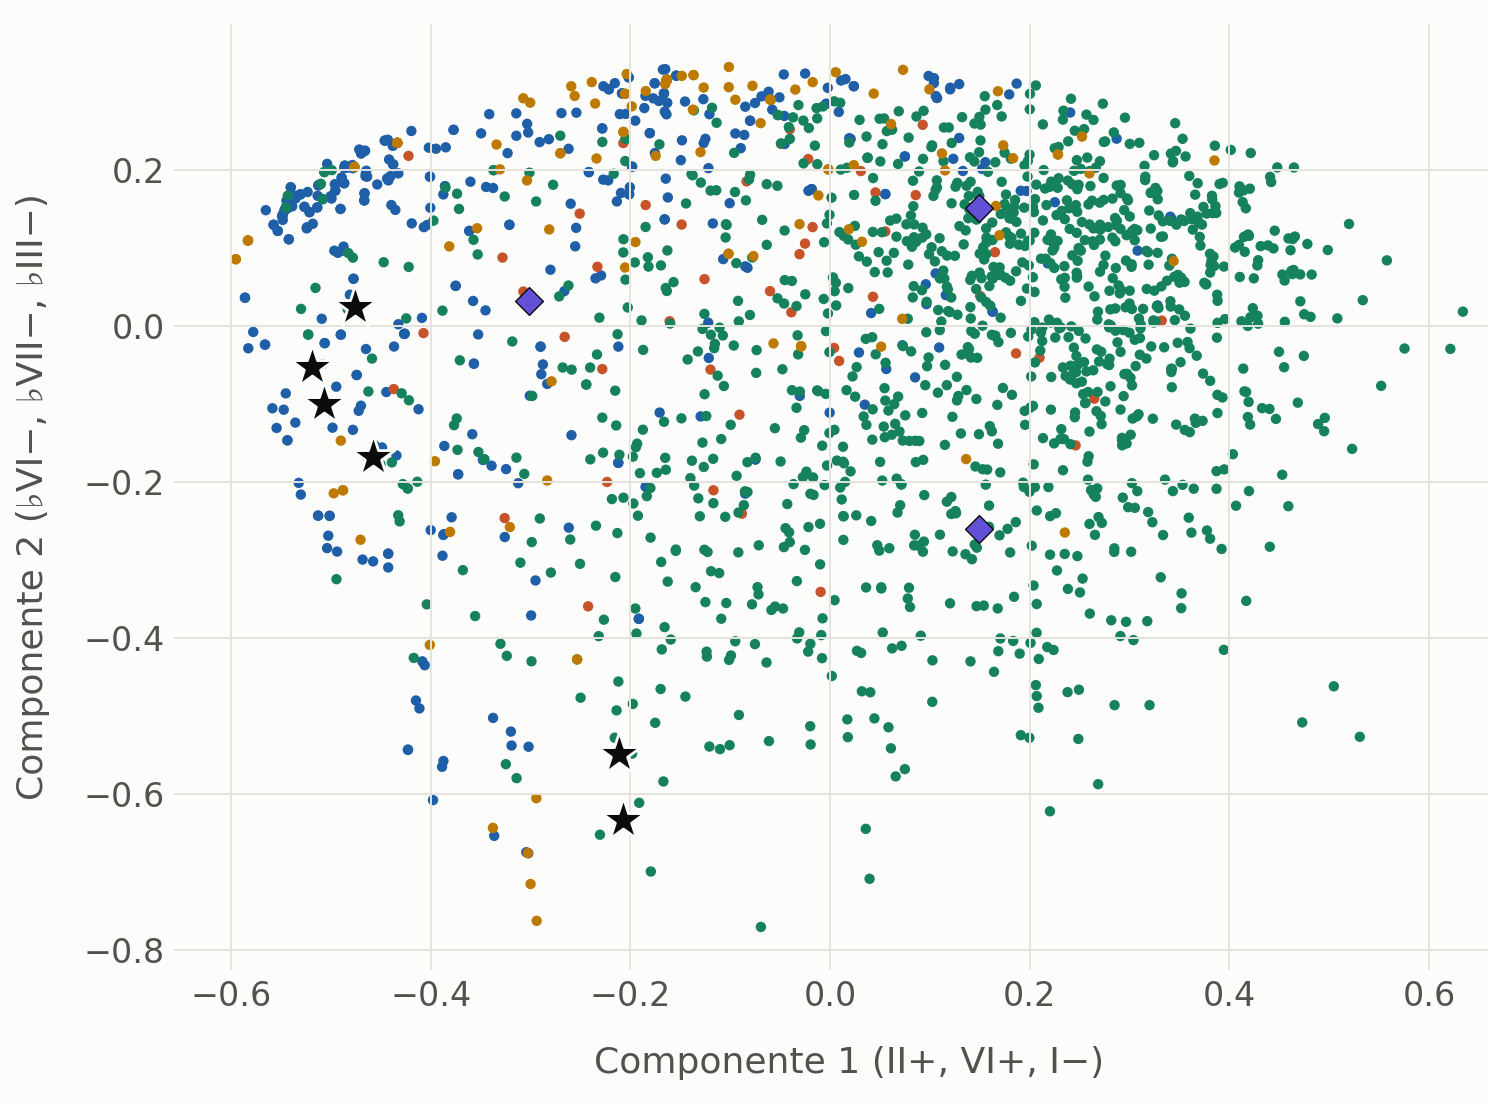
\includegraphics[width=\textwidth]{1b_armonia_mapa_fundamentales.png}
  \caption{Mapa de fundamentales. Puntos del fondo: rock (azul, RS~200, 400 piezas), práctica común (rojo, Kostka-Payne, 46), jazz (verde, iRealPro, 1186) y pop (naranja, Hooktheory, 121). Estrellas: la banda; rombos: Primus. Puntos cercanos tienen repartos de fundamentales parecidos; los ejes son componentes principales (entre paréntesis, los grados que más pesan).}\label{fig:mapa}
\end{figure}

Frente al pop de Hooktheory, la banda queda a una distancia de Jensen-Shannon de 0.40 a 0.59, cuando los nueve álbumes de
pop entre sí no pasan de 0.07. Los ejes de Lendvai muestran rasgos que el círculo de quintas no ve: en Sarniezz, el 24\,\%
de los cambios de la partitura queda dentro del eje de tónica (I $\leftrightarrow$ \fl III, Mi $\leftrightarrow$ Sol), una
sustitución y no un movimiento por quintas; las canciones con cuartos de tono se mueven entre un eje de Lendvai y uno
neutro (Mata Zyklek D $\leftrightarrow$ D--S, Yor Zarad T $\leftrightarrow$ D--S).

La tabla~\ref{tab:funciones} resume el movimiento armónico de cada canción. Tres patrones se distinguen: los pedales
(Mata Zyklek, Utzp y Angor), casi sin cambios de fundamental y con más del 90\,\% del tiempo en función de tónica; el
vaivén modal de Fabienk y Sarniezz, con decenas de cambios y alrededor de un tercio del tiempo en dominante modal
(\fl VII, sin sensible); y el vaivén microtonal de Yor Zarad, cuyos cambios son todos entre I y \fl II+, fuera de la tabla
de progresiones de Piston.

\begin{table}[ht]
  \centering\small
  \caption{Funciones y progresiones (compases confiables). T, D, N: porcentaje del tiempo en función de tónica,
  dominante y neutra.}\label{tab:funciones}
  \begin{tabular}{@{}lrrrrrl@{}}
    \toprule
    Canción & Cambios & Por quintas & T & D & N & Progresión más frecuente \\
    \midrule
    Mata Zyklek & 2 & 100\,\% & 92.7 & 7.3 & 0 & I5 $\to$ Vsus4 $\to$ I \\
    Fabienk & 86 & 51\,\% & 63.1 & 36.9 & 0 & \fl VII $\to$ \fl III \\
    Sarniezz & 56 & 59\,\% & 66.6 & 29.5 & 3.9 & \fl III $\leftrightarrow$ \fl VIIsus2 \\
    Yor Zarad & 11 & 0\,\% & 85.6 & 0 & 14.4 & I5 $\leftrightarrow$ \fl II+5 \\
    Utzp & 9 & 22\,\% & 97.7 & 2.3 & 0 & \fl VIIsus2 $\to$ Iaum \\
    Angor & 0 & — & 100 & 0 & 0 & — \\
    \bottomrule
  \end{tabular}
\end{table}

\section{Melodía: cuartos de tono como grados fijos}\label{sec:res-melodia}

La tabla~\ref{tab:cuartos} y la figura~\ref{fig:uso} muestran cómo usa cada canción los cuartos de tono.

\begin{figure}[htbp]
  \centering
  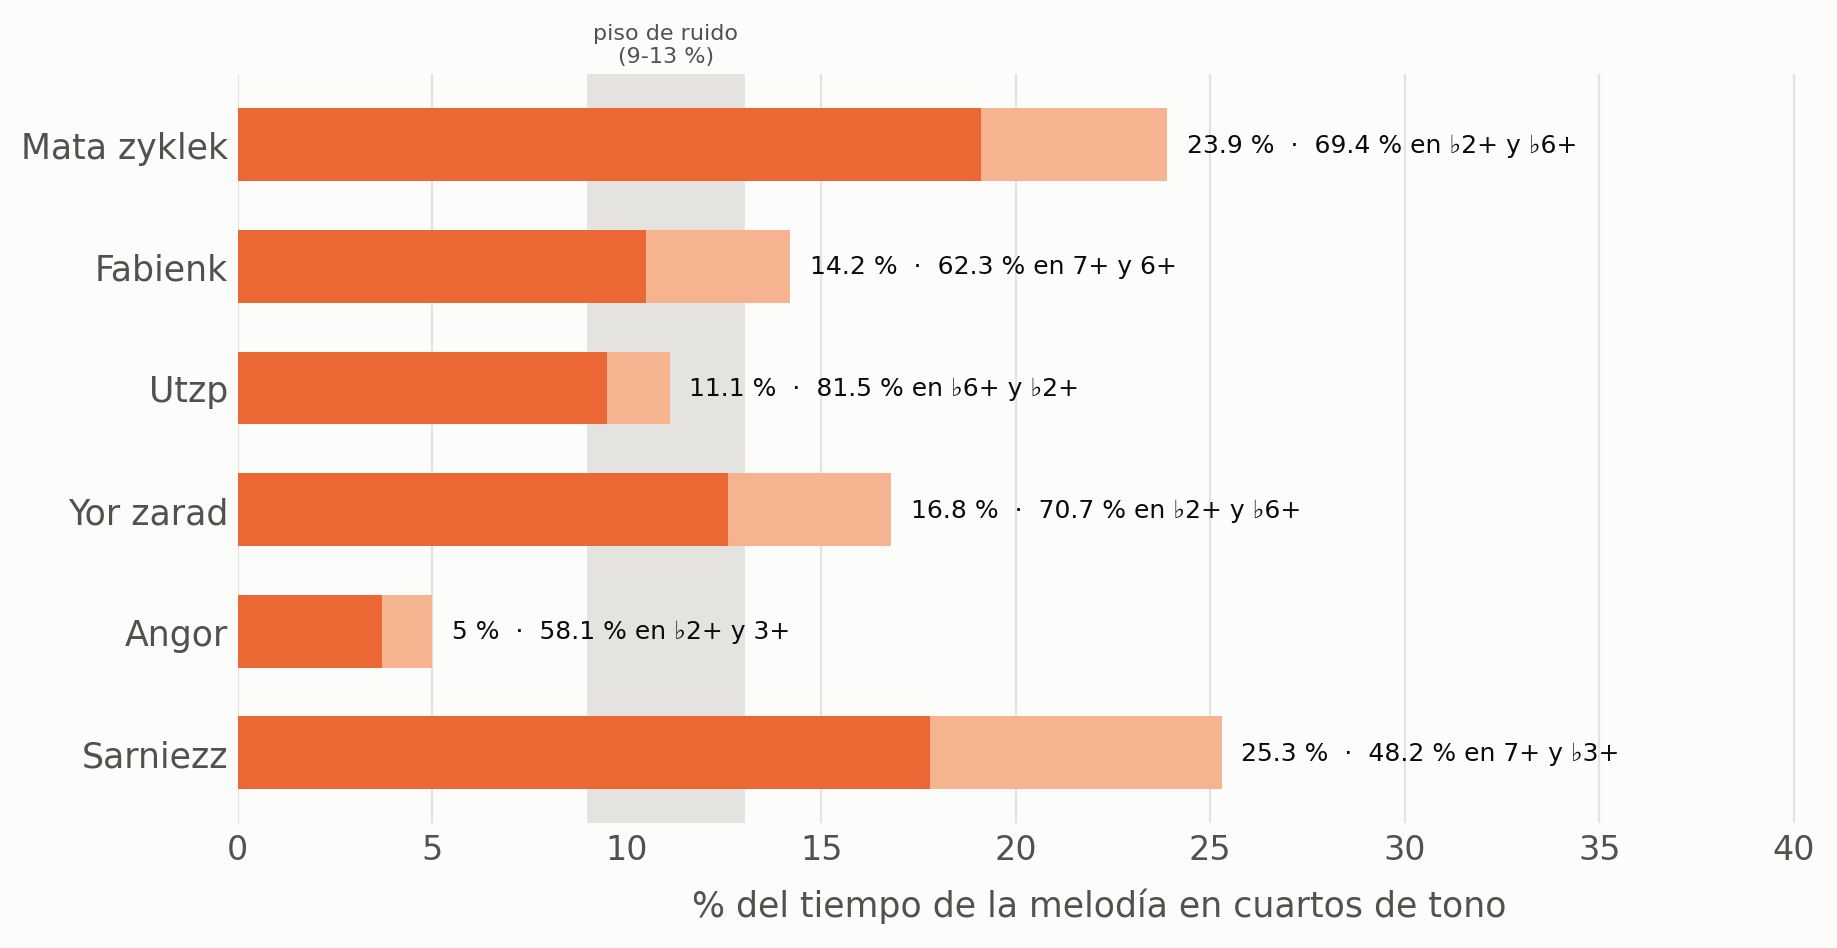
\includegraphics[width=0.9\textwidth]{2a_melodia_uso_cuartos_de_tono.png}
  \caption{Cuartos de tono en la melodía (\% del tiempo). Oscuro: como grado sostenido; claro: como adorno. Franja gris: piso de ruido medido en Primus (9--13\,\%). A la derecha de cada barra, la fracción que cae en los dos grados más usados.}\label{fig:uso}
\end{figure}

\begin{table}[ht]
  \centering
  \caption{Uso de los cuartos de tono en la melodía (\% del tiempo de la voz aguda).}\label{tab:cuartos}
  \begin{tabular}{@{}lcrrrr@{}}
    \toprule
    Canción & Centro & \shortstack{En \cuarto{}\\de tono} & \shortstack{Como\\grado} & \shortstack{Como\\inflexión} & \shortstack{En los dos grados\\más usados} \\
    \midrule
    Mata Zyklek & Sol & 23.9 & 19.1 & 4.8 & 69.4 \\
    Fabienk & Mi & 14.2 & 10.5 & 3.7 & 62.3 \\
    Utzp & Mi & 11.1 & 9.5 & 1.6 & 81.5 \\
    Yor Zarad & Sol & 16.8 & 12.6 & 4.2 & 70.7 \\
    Angor & Sol & 5.0 & 3.7 & 1.3 & 58.1 \\
    Sarniezz & Mi & 25.3 & 17.8 & 7.5 & 48.2 \\
    \midrule
    Primus (control) & & 9--13 & & & 28--37 \\
    \bottomrule
  \end{tabular}
\end{table}

Entre el 48 y el 82\,\% de los cuartos de tono de cada canción caen en solo dos grados, que vuelven en cada vuelta del
loop; en Primus están repartidos (28--37\,\%). Son grados de la escala, no adornos: la mayor parte del tiempo en cuarto de
tono es como grado sostenido. Angor, con 5\,\%, queda por debajo del piso de ruido y no cuenta. Las mismas barras para
las 36 canciones y la escala de cada una están en el apéndice (figuras~\ref{fig:g-uso} a~\ref{fig:g-escalas2}).

El círculo de 24-EDO (figura~\ref{fig:circulo}) muestra qué escalas forman esos grados. Aparecen dos familias:
\begin{itemize}
  \item \textbf{Frigia:} \fl2+ y \fl6+ sobre un frigio (Mata Zyklek, Yor Zarad y Utzp).
  \item \textbf{Dórica:} 7+, 6+ y \fl3+ sobre un dórico (Sarniezz: 7+ y \fl3+; Fabienk: 7+ y 6+).
\end{itemize}

\begin{figure}[htbp]
  \centering
  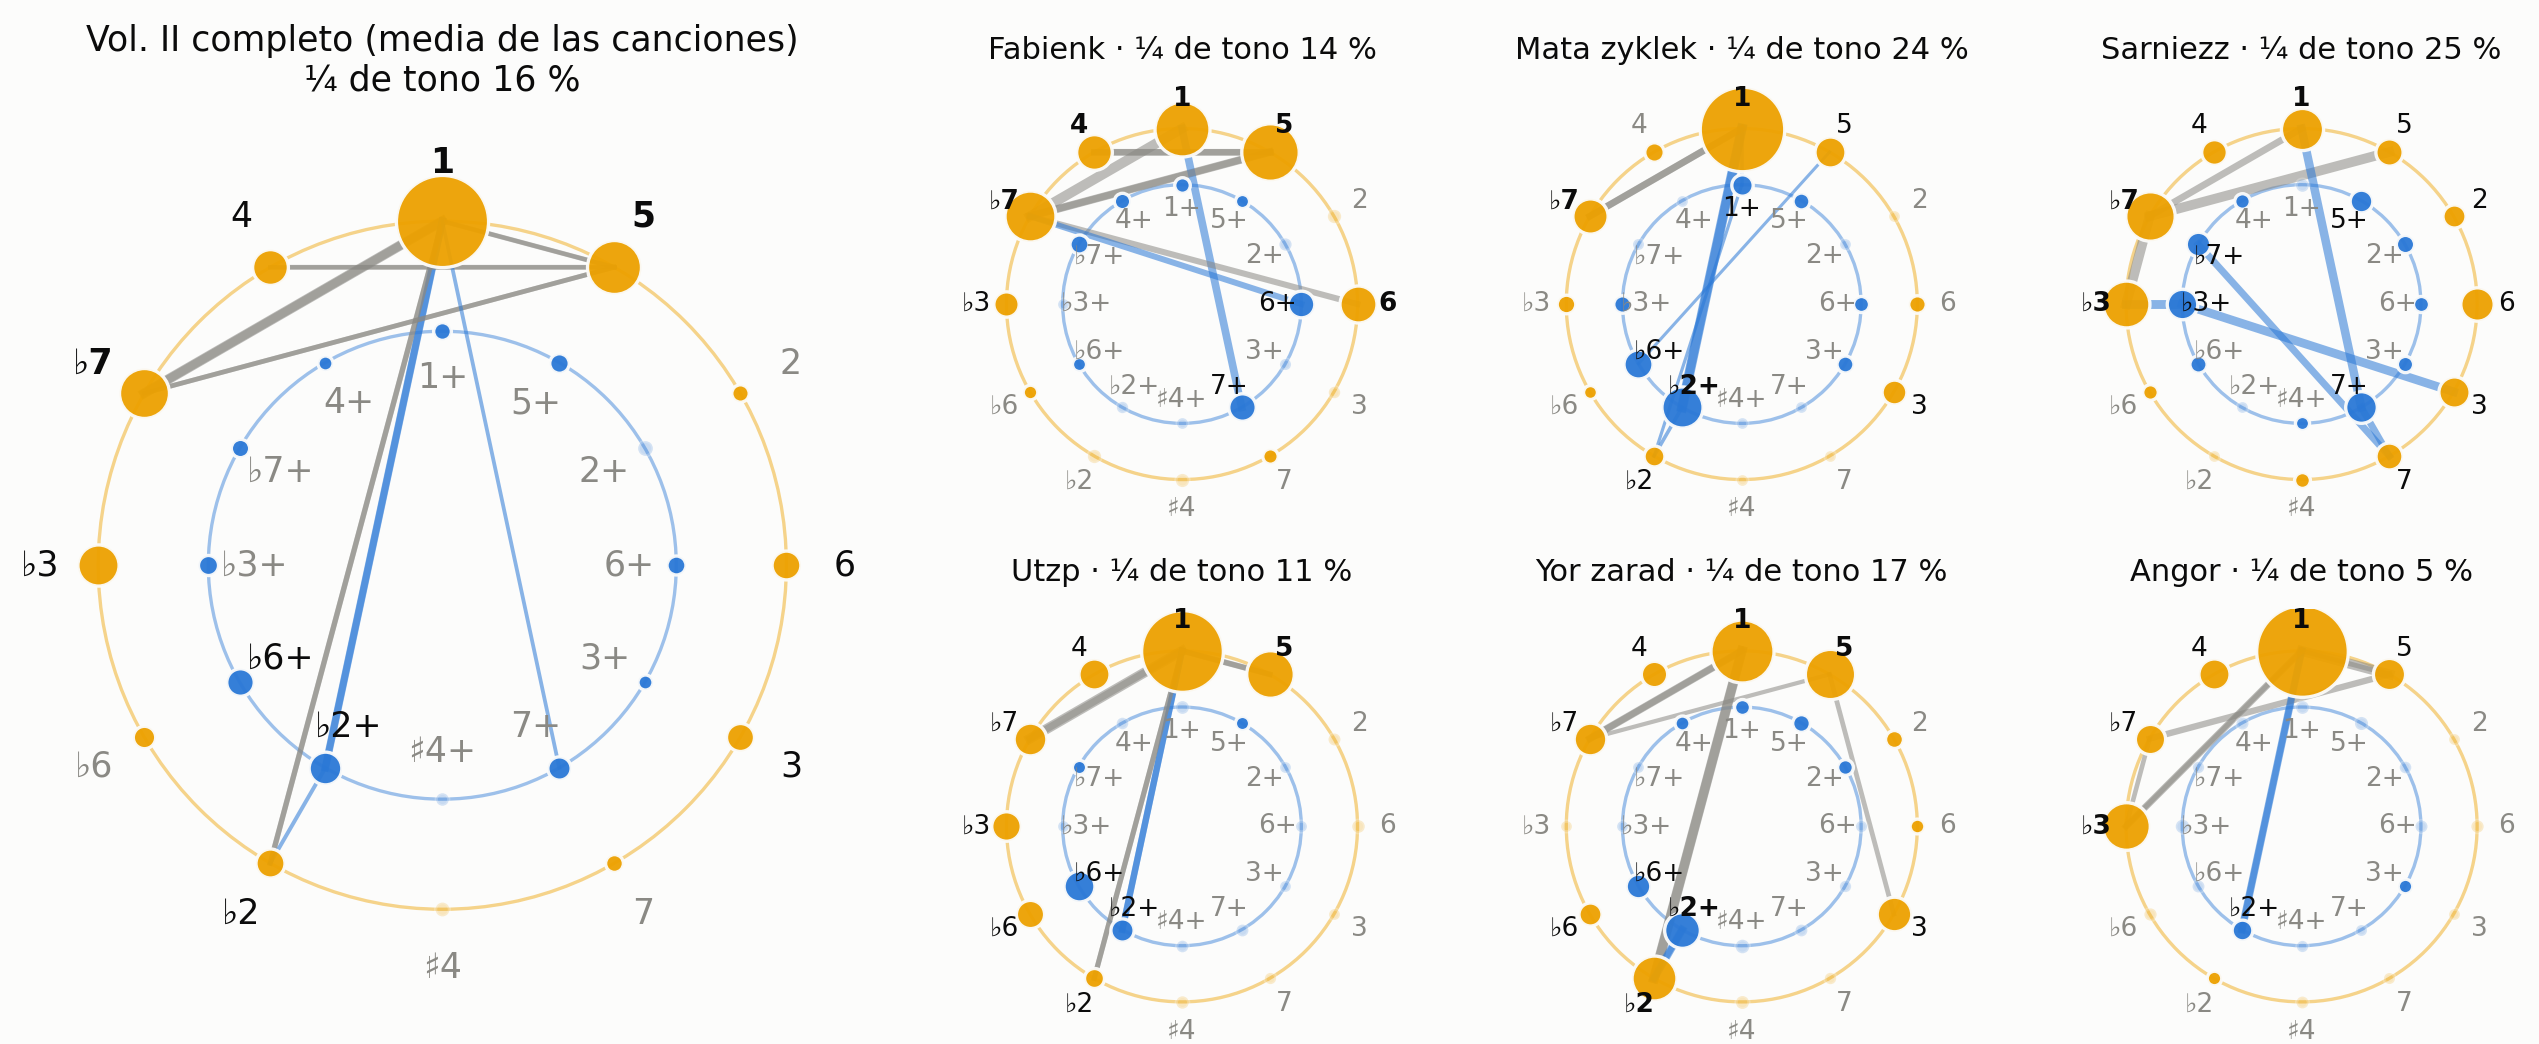
\includegraphics[width=\textwidth]{2b_melodia_circulo_24edo.png}
  \caption{Círculo de quintas en 24-EDO: el álbum (izquierda) y cada canción. Anillo amarillo: campo regular; anillo azul: campo de cuarto de tono. Área del punto: tiempo melódico en el grado; líneas grises: pasos dentro de un campo; azules: pasos entre campos.}\label{fig:circulo}
\end{figure}

La tabla~\ref{tab:familias} compara esas familias con los corpus. La frigia no es exclusiva de la banda: es el par más
común del radif persa y el de King Gizzard. Lo que ningún corpus medido tiene es la familia dórica. El corpus indostánico
no aporta cuartos de tono, porque sus 22 \emph{shrutis} caen todos en grados regulares al pasarlos a 24-EDO.

\begin{table}[ht]
  \centering\small
  \caption{Los dos grados en cuarto de tono más usados de cada pieza, por corpus.}\label{tab:familias}
  \begin{tabular}{@{}lrrr@{}}
    \toprule
    & \shortstack{Con cuartos\\de tono ($\ge 2$\,\%)} & \shortstack{Familia frigia\\(\fl2+, \fl6+)} & \shortstack{Familia dórica\\(7+, 6+, \fl3+)} \\
    \midrule
    Radif Corpus & 190 de 229 & 43 & 0 \\
    Indostánico & 0 de 50 & — & — \\
    King Gizzard (medido) & 9 de 9 & 5 & 0 \\
    Angine de Poitrine & 6 de 6 & 3 & 2 \\
    \bottomrule
  \end{tabular}
\end{table}

\subsection{El círculo en movimiento}\label{sec:circulo-vivo}

Para la presentación se exportó un fragmento de Mata Zyklek (de 0:42 a 1:12) que anima las notas sobre el círculo,
sincronizadas con el audio. Con tónica Sol, las voces giran sobre Sol y Sol\sh+ (\fl2+), el cuarto de tono del riff.
Frente a la referencia corregida de oído, la herramienta da el mismo grado el 90\,\% del tiempo en la voz aguda y el
88\,\% en la grave, y cuando falla lee Sol\sh+ como Sol: se queda corta, no inventa cuartos de tono.

La exportación exigió dos correcciones. Las notas iban adelantadas, porque la ventana centrada de 4096 muestras ya «ve» la
nota cuando empieza a cubrirla; el mejor acuerdo con pYIN se obtuvo atrasándolas 60~ms en la voz aguda y 55~ms en la
grave, sin deriva a lo largo de la canción. Y se quitaron las notas de menos de 0.15~s de grados que suman menos del 2\,\%
del tiempo de la voz: tres notas de Do que eran errores de quinta (Do es el tercer armónico de Fa).

\section{Desplazamiento de campos}\label{sec:res-haba}

Levi McClain y David Bennett sostienen que la banda usa los cuartos de tono de forma «horizontal», en la melodía, y casi
nunca «vertical», en los acordes, como proponía Hába \citep{mcclain2026,bennett2026}. Para ponerlo a prueba se midió la
\emph{mezcla vertical} $V$: en una rejilla de 20~ms, la fracción del tiempo en que suenan a la vez la voz aguda y el bajo
y están en campos distintos (sección~\ref{sec:campos}). El modelo nulo desplaza el bajo en bloque un tiempo al azar (al
menos 2~s, de forma circular), lo que conserva cuántos cuartos de tono tiene cada voz y su ritmo, pero rompe su
coordinación; $p$ es la fracción de desplazamientos con una mezcla igual o menor que la observada.

\begin{table}[ht]
  \centering
  \caption{Mezcla vertical de campos: observada frente a la esperada por azar.}\label{tab:haba}
  \begin{tabular}{@{}llrrr@{}}
    \toprule
    Grupo & Canción & Observada & Azar & $p$ \\
    \midrule
    Banda & Sarniezz & 15.4\,\% & 38.5\,\% & $< 0.002$ \\
    & Mata Zyklek & 12.7\,\% & 35.8\,\% & $< 0.002$ \\
    & Fabienk & 12.7\,\% & 25.2\,\% & $< 0.002$ \\
    & Yor Zarad & 17.8\,\% & 33.0\,\% & $< 0.002$ \\
    & Utzp & 11.4\,\% & 20.3\,\% & $< 0.002$ \\
    & Angor & 4.7\,\% & 8.0\,\% & 0.006 \\
    \midrule
    Primus & Tommy the Cat & 19.6\,\% & 22.7\,\% & 0.006 \\
    & My Name Is Mud & 20.8\,\% & 21.8\,\% & 0.218 \\
    & Jerry Was a Race Car Driver & 18.2\,\% & 20.6\,\% & $< 0.002$ \\
    \midrule
    King Gizzard & Flying Microtonal Banana & 5.8\,\% & 11.6\,\% & $< 0.002$ \\
    & Doom City & 24.5\,\% & 33.7\,\% & 0.020 \\
    & Melting & 16.9\,\% & 26.5\,\% & 0.002 \\
    \bottomrule
  \end{tabular}
\end{table}

En la banda, la mezcla observada es entre un 35 y un 60\,\% de la esperada por azar; en Primus, entre un 86 y un 95\,\%
(tabla~\ref{tab:haba}). Es decir, cuando la guitarra está en un cuarto de tono, el bajo tiende a acompañarla en el mismo
campo, o a callar, mucho más de lo que daría la casualidad: la banda evita mezclar campos en vertical, como Hába. En
Primus, donde todo cuarto de tono es error de medición, la mezcla queda cerca del azar. En Mata Zyklek y Fabienk, además,
los cuartos de tono caen en el pulso menos que las notas regulares (16 frente a 29\,\%, y 15 frente a 34\,\%; $p < 0.002$
en ambos), lo que es coherente con un uso melódico.

El círculo de la figura~\ref{fig:circulo} ya separaba los dos campos: el anillo amarillo es el campo regular y el azul,
el de cuarto de tono, y la mayoría de los pasos melódicos frecuentes quedan dentro de un mismo campo. La
figura~\ref{fig:campos-tiempo} añade el tiempo: los cuartos de tono no se reparten de forma pareja, sino que se agrupan en
tramos de cada canción, y la mezcla de campos entre guitarra y bajo aparece en muchos compases, pero baja: casi siempre ocupa una parte
pequeña del compás, con pocos picos. La
figura~\ref{fig:campos-resumen} compara las tres pruebas (mezcla evitada, pasos de cuarto de tono entre las notas que ya
tocan uno y presencia en el pulso) en la banda, los repertorios comparados y Primus. En la primera, las seis canciones de
la banda evitan la mezcla entre un 40 y un 65\,\%, lejos del rango del control; los repertorios se reparten a ambos lados,
y algunos llegan al nivel de la banda: «Open Water» y «Flying Microtonal Banana» de King Gizzard, «The Black Page \#1»
de Zappa y «The Runaway» de Gentle Giant. En la figura, un punto vacío indica $p \geq 0.003$, el umbral corregido por
Bonferroni para unas 18 canciones; por eso Angor y «Tommy the Cat» ($p = 0.006$ en la tabla~\ref{tab:haba}) aparecen
como no significativos.

Los acordes dan otra forma de ver la separación, porque una tríada con tercera neutra mezcla campos por construcción
(proposición~\ref{prop:neutra}). En los compases confiables, la herramienta lee la calidad «n» en 2 de los 658 compases de
la banda (0.3\,\%), uno en Utzp y uno en Sarniezz, y en 1 de los 196 de Primus (0.5\,\%), que es el piso de error. King
Gizzard la usa más: 42 de 1120 compases (3.8\,\%), sobre todo en «Melting» (20 de 110), «Nuclear Fusion» (11 de 124) y
«Billabong Valley» (7 de 113). Zappa, King Crimson y Gentle Giant quedan entre el 0.6 y el 1.7\,\%. La banda no arma
acordes con tercera neutra, lo que es coherente con un uso melódico de los cuartos de tono.

\begin{figure}[htbp]
  \centering
  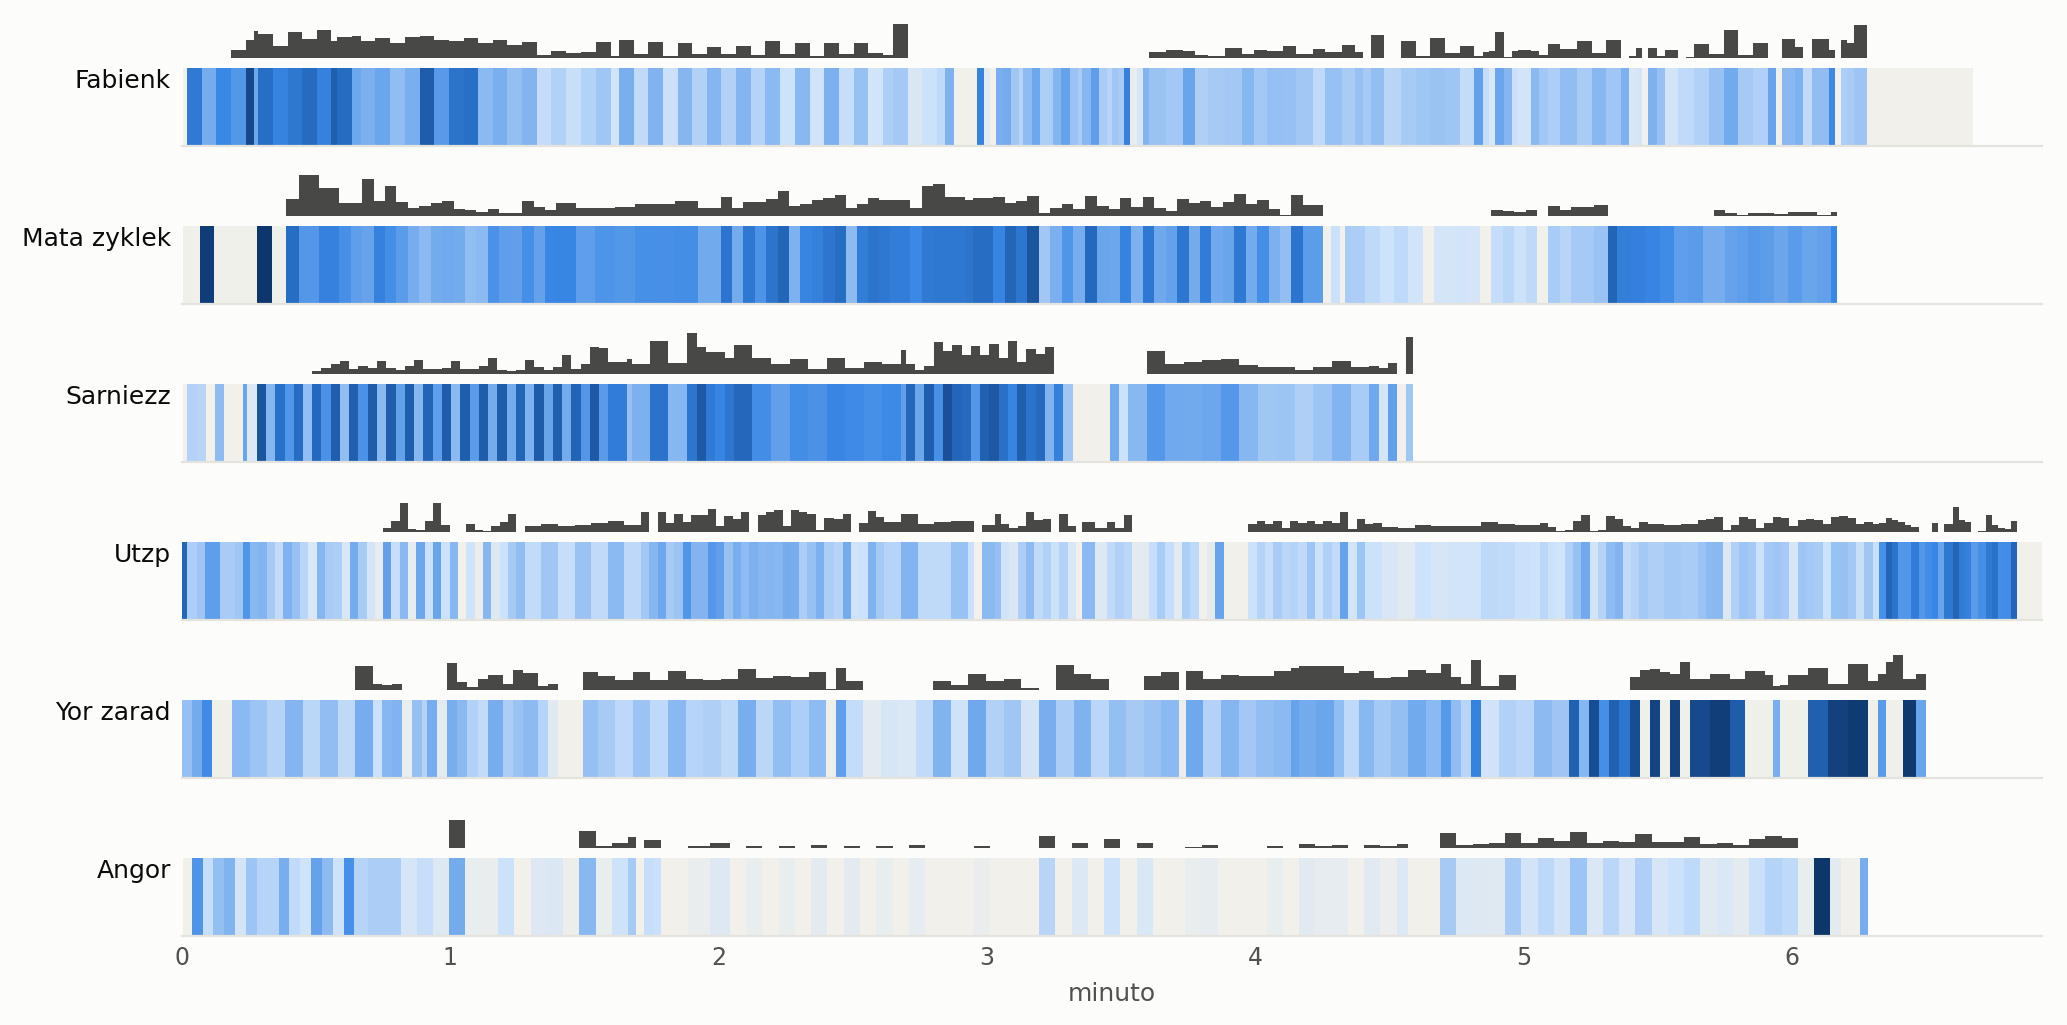
\includegraphics[width=\textwidth]{g_campos_tiempo.png}
  \caption{Cuartos de tono a lo largo de cada canción (eje en minutos). Franja: porcentaje de cada compás en cuarto de tono, de blanco (0\,\%) a azul oscuro (60\,\%). Barras negras: compases con guitarra y bajo en campos distintos (alto completo = 50\,\% o más).}\label{fig:campos-tiempo}
\end{figure}

\begin{figure}[htbp]
  \centering
  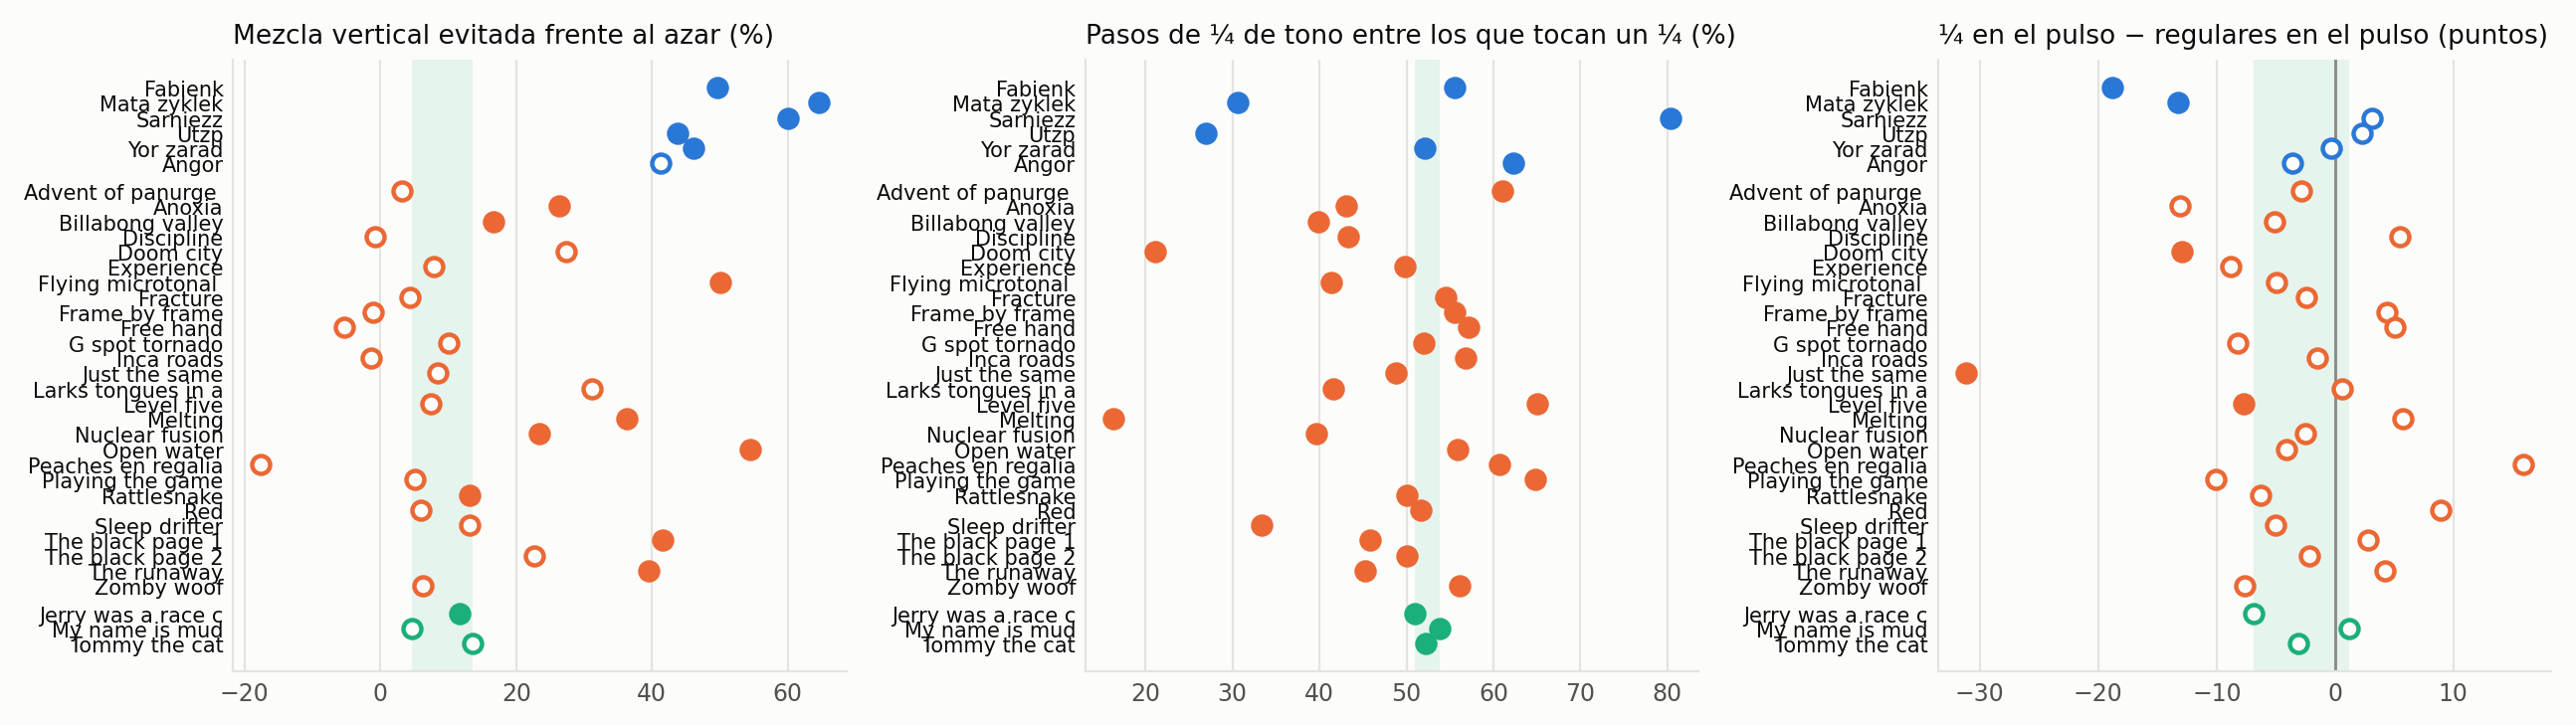
\includegraphics[width=\textwidth]{g_campos_resumen.png}
  \caption{Tres pruebas de separación de campos, una canción por fila. Izquierda: mezcla vertical evitada frente al azar (\%); centro: pasos de cuarto de tono entre las notas que ya están en cuarto de tono (\%); derecha: diferencia entre los cuartos de tono y las notas regulares que caen en el pulso (puntos). Azul: la banda; naranja: repertorios comparados (King Gizzard, Zappa, King Crimson y Gentle Giant); verde: Primus. Círculo vacío: no significativo ($p \ge 0.003$); franja verde: rango del control.}\label{fig:campos-resumen}
\end{figure}

\section{Metro: ciclos de 5 y de 7}\label{sec:res-metro}

\begin{table}[ht]
  \centering
  \caption{Mejor periodo de repetición $R(\ell)$ de cada canción.}\label{tab:ciclos}
  \begin{tabular}{@{}lrrr@{}}
    \toprule
    Canción & Tempo (BPM) & Mejor periodo (corcheas) & $R$ \\
    \midrule
    Mata Zyklek & 94 & 20 (dos compases de 5/4) & 0.82 \\
    Fabienk & 129 & 28 (dos compases de 7/4) & 0.87 \\
    Yor Zarad & 108 & 28 & 0.80 \\
    Angor & 99 & 24 & 0.83 \\
    Sarniezz & 115 & 32 & 0.83 \\
    Utzp & 129 & 32 & 0.87 \\
    \midrule
    Tommy the Cat (Primus) & 129 & 8 & 0.44 \\
    Jerry Was a Race Car Driver (Primus) & 123 & 8 & 0.45 \\
    \bottomrule
  \end{tabular}
\end{table}

El riff de Mata Zyklek se repite cada 20 corcheas: dos compases de 10 corcheas, es decir, de 5/4. El de Fabienk, cada 28:
dos compases de 7/4 (tabla~\ref{tab:ciclos} y figura~\ref{fig:ciclos}). Son los compases que menciona la banda y los que
planteaba la hipótesis. Sarniezz y Utzp, en cambio, van en 4, con picos en 32 corcheas. Los ciclos de la banda son mucho
más estables que los de Primus ($R \approx 0.8$ frente a 0.44). Varias canciones mezclan compases dentro de la misma
pieza: Fabienk pasa el 53\,\% del tiempo en compases de 7, el 18\,\% en 4 y el 9\,\% en 3. El periodo de 28 corcheas de
Yor Zarad es, como en Fabienk, un par de compases de 7/4: el 7 domina el centro de la canción y el 4 aparece al principio
y al final. El de 24 corcheas de Angor es un par de compases de 6/4, el compás de 83 de sus 113 compases; Angor no
tiene referencia de oído, así que esta lectura no está contrastada.

\begin{figure}[htbp]
  \centering
  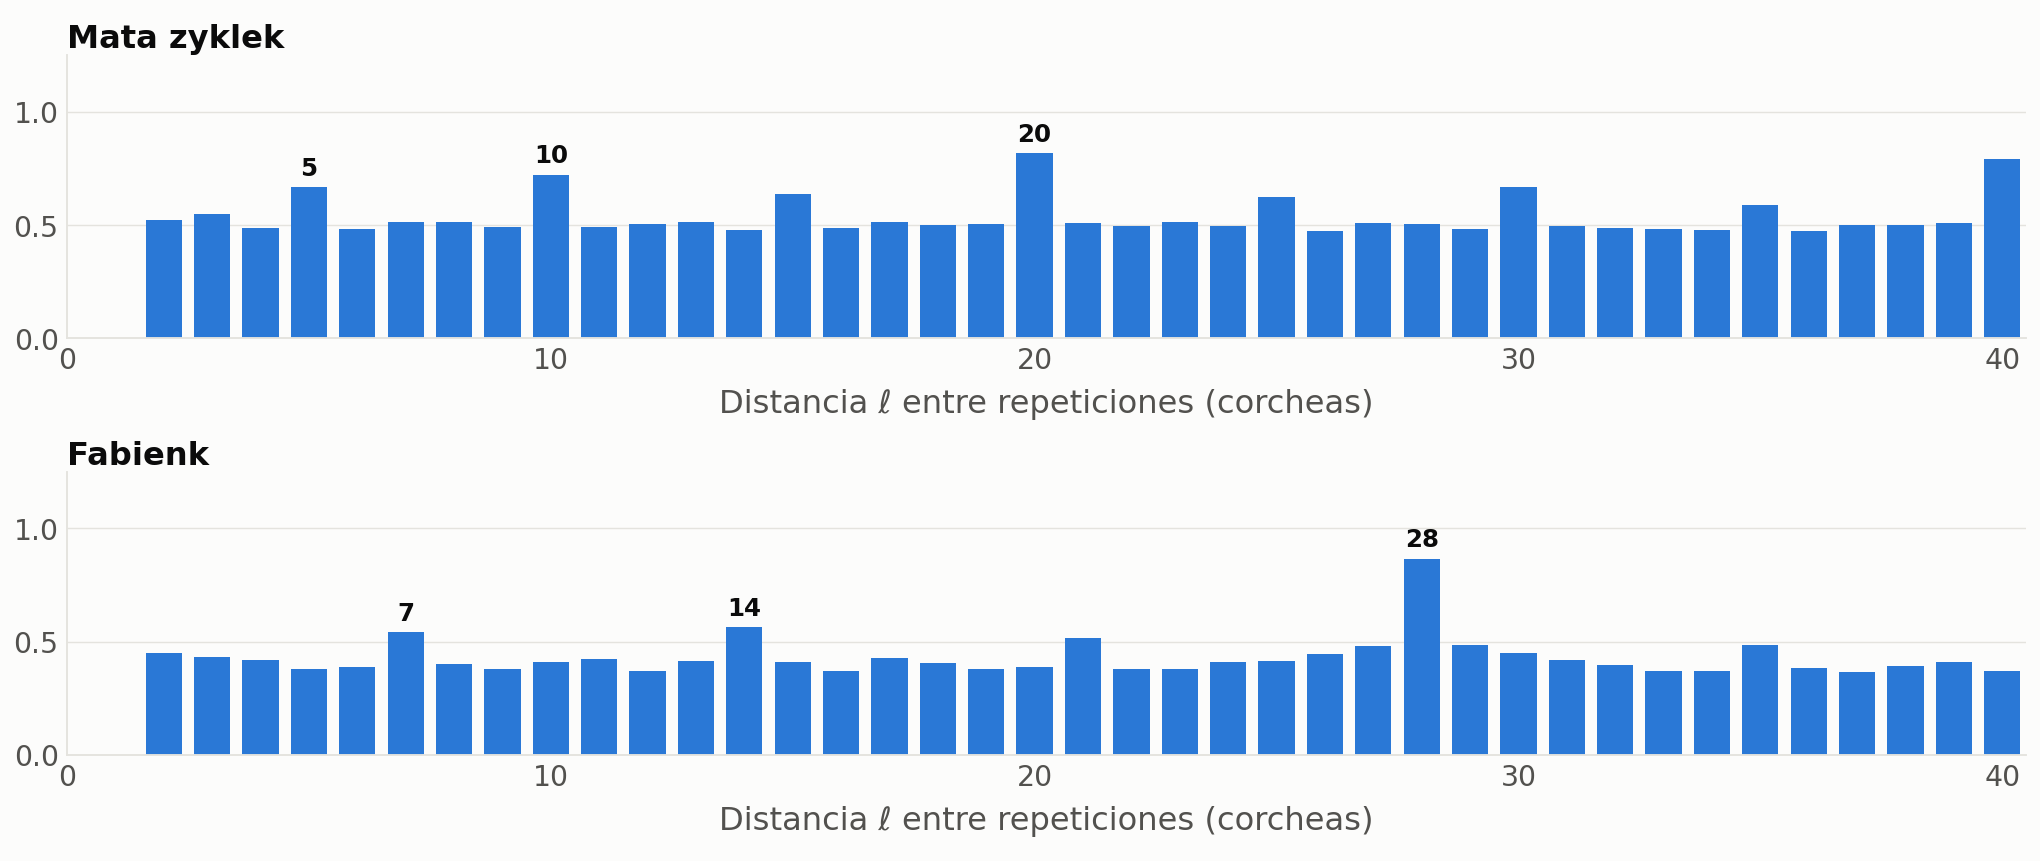
\includegraphics[width=0.75\textwidth]{3a_sintesis_ciclos_metricos.png}
  \caption{Repetición $R(\ell)$ en Mata Zyklek y Fabienk según la distancia $\ell$ en corcheas. Un pico alto y aislado es un ciclo largo y estable: 20 y 28 corcheas.}
  \label{fig:ciclos}
\end{figure}

La figura~\ref{fig:ciclos-todos} extiende la figura~\ref{fig:ciclos} a las 36 canciones. Las de la banda tienen picos
altos sobre un fondo también alto, porque el looper repite casi idéntico; las de Primus y de los repertorios de rock
progresivo tienen picos más bajos sobre un fondo bajo. El radar de la figura~\ref{fig:radar-ritmico} resume el perfil
rítmico de cada grupo con la mediana de sus canciones: la banda destaca en ostinato, más que cualquier repertorio, y
Fabienk, que se muestra aparte, es la única con ciclos de largo desigual y con compás irregular y cambiante altos; el
pulso constante es común a todos los grupos.

\begin{figure}[htbp]
  \centering
  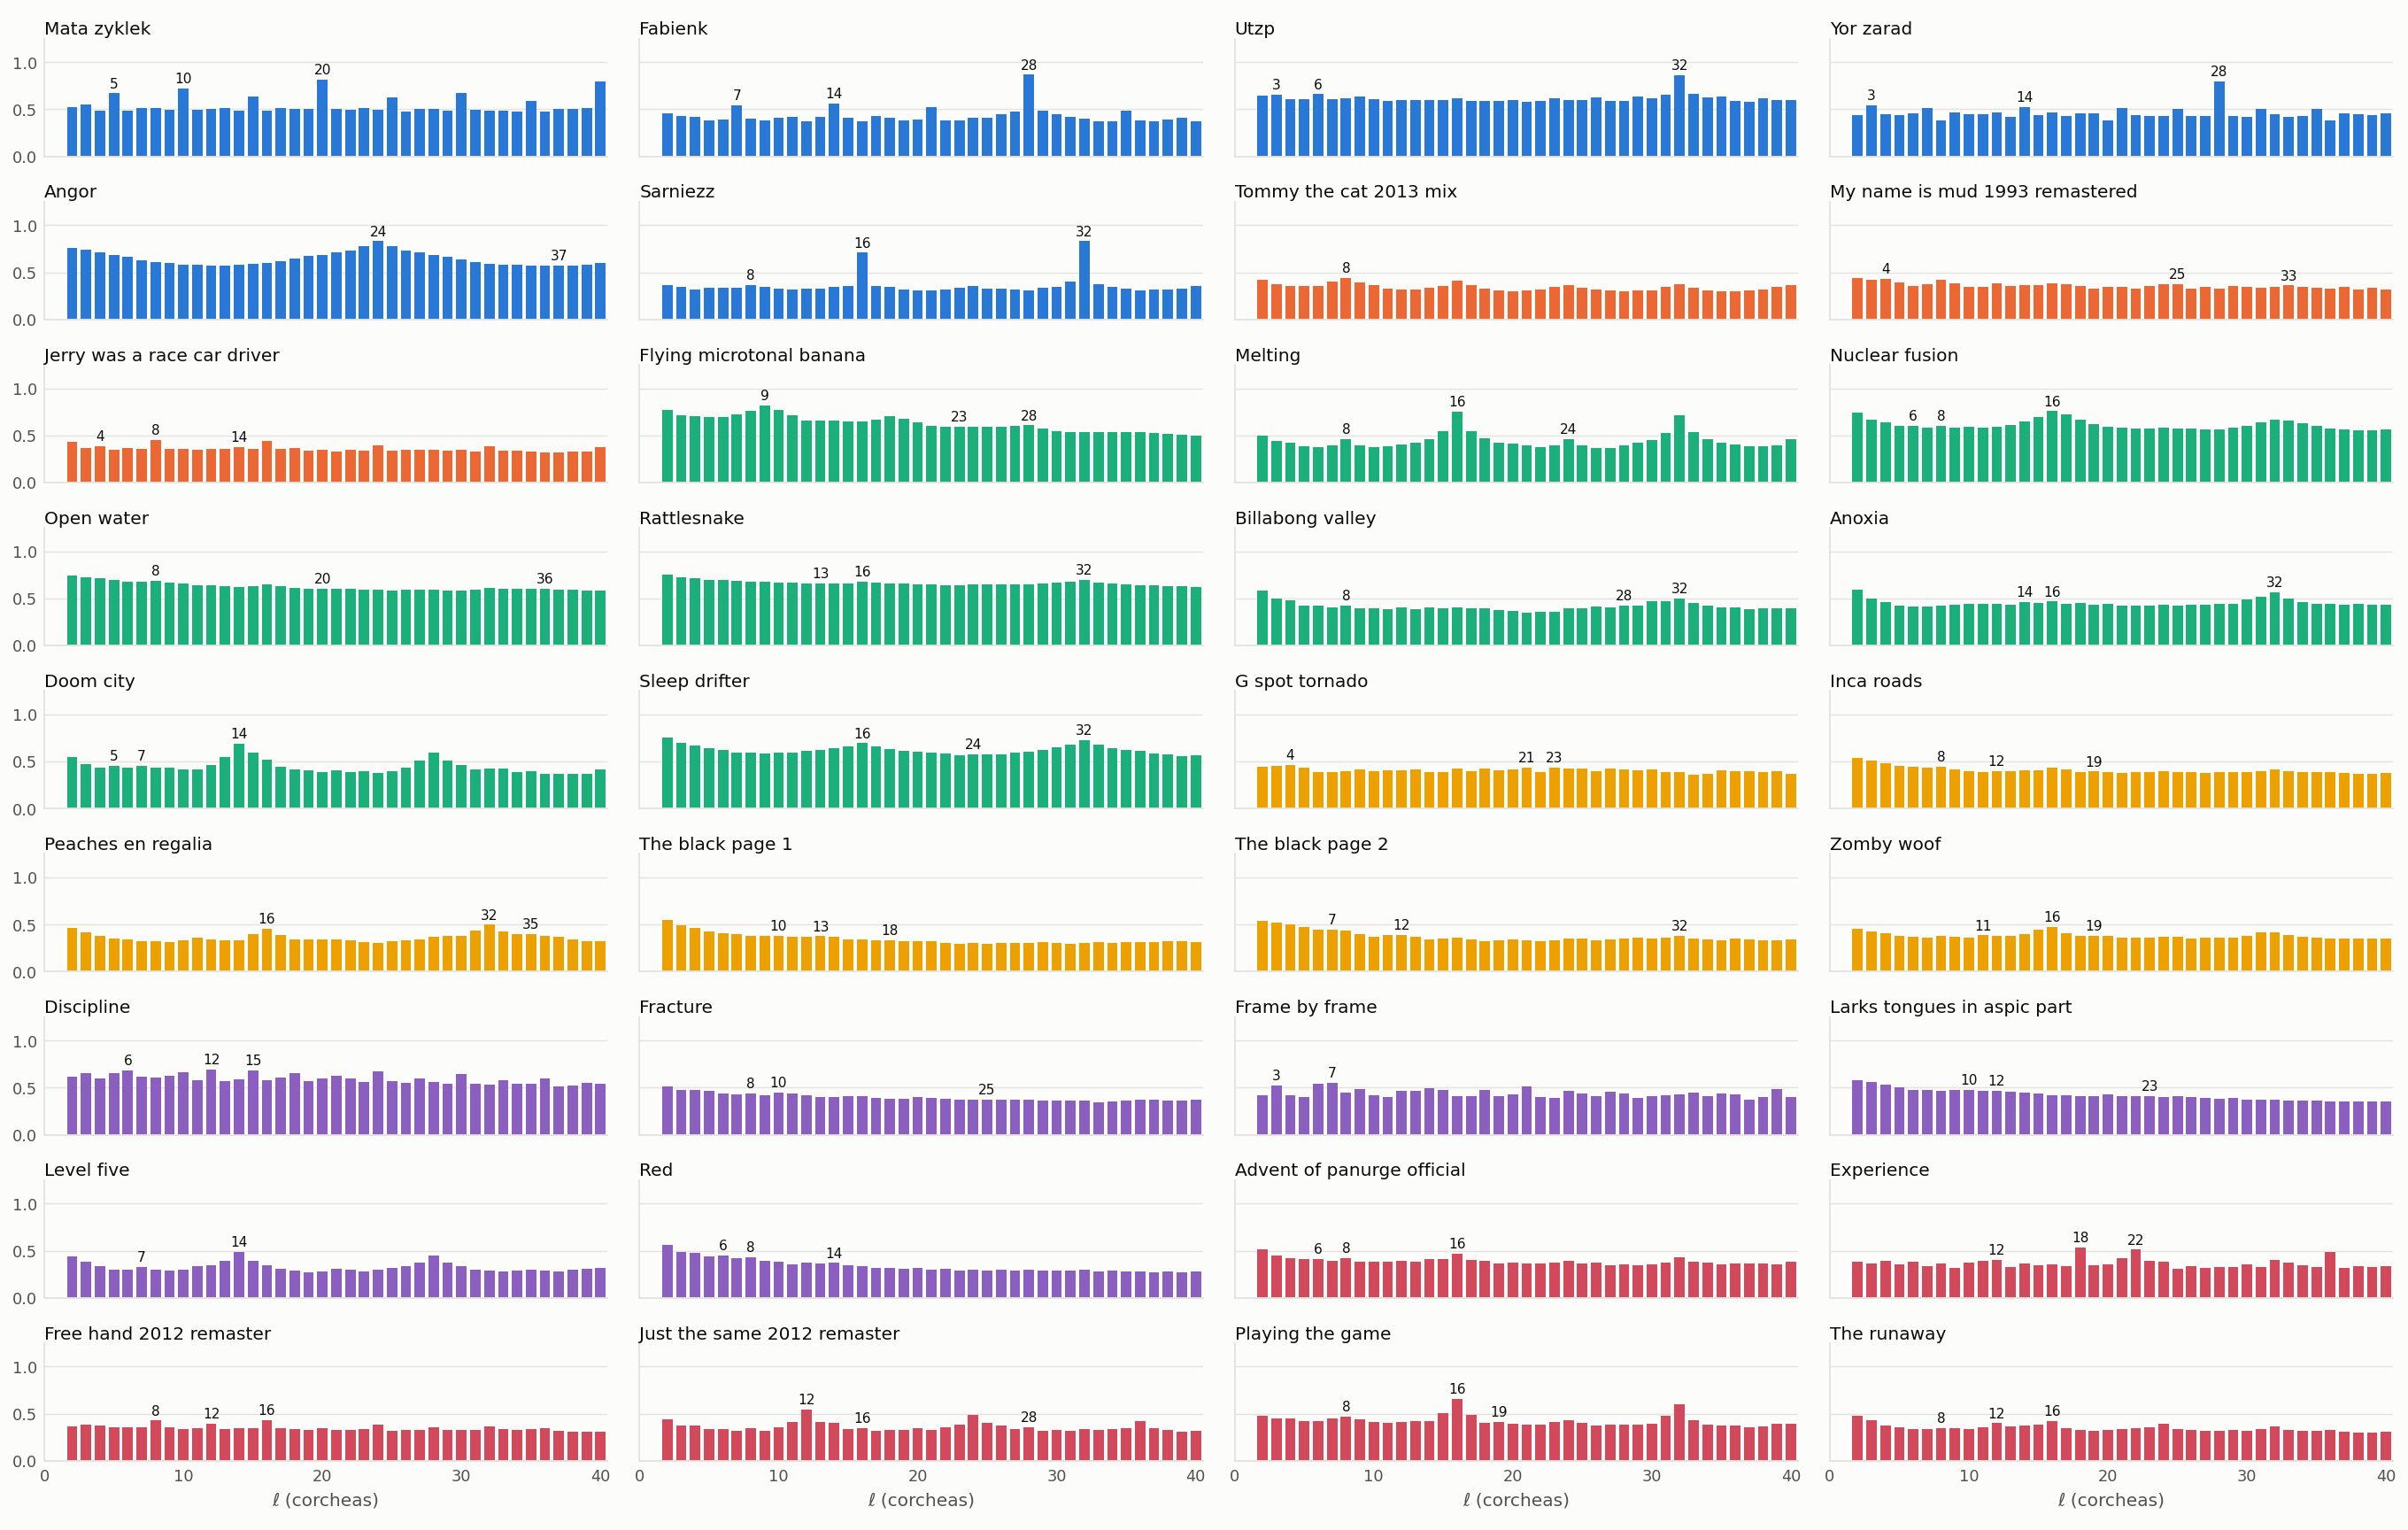
\includegraphics[width=\textwidth]{g_ciclos_metricos.png}
  \caption{Repetición $R(\ell)$ de las 36 canciones (eje $x$: $\ell$ en corcheas; eje $y$: $R$ de 0 a 1). Color por artista: azul, la banda; naranja, Primus; verde, King Gizzard; amarillo, Zappa; violeta, King Crimson; rojo, Gentle Giant. Las cifras sobre las barras son los mejores periodos.}\label{fig:ciclos-todos}
\end{figure}

\begin{figure}[htbp]
  \centering
  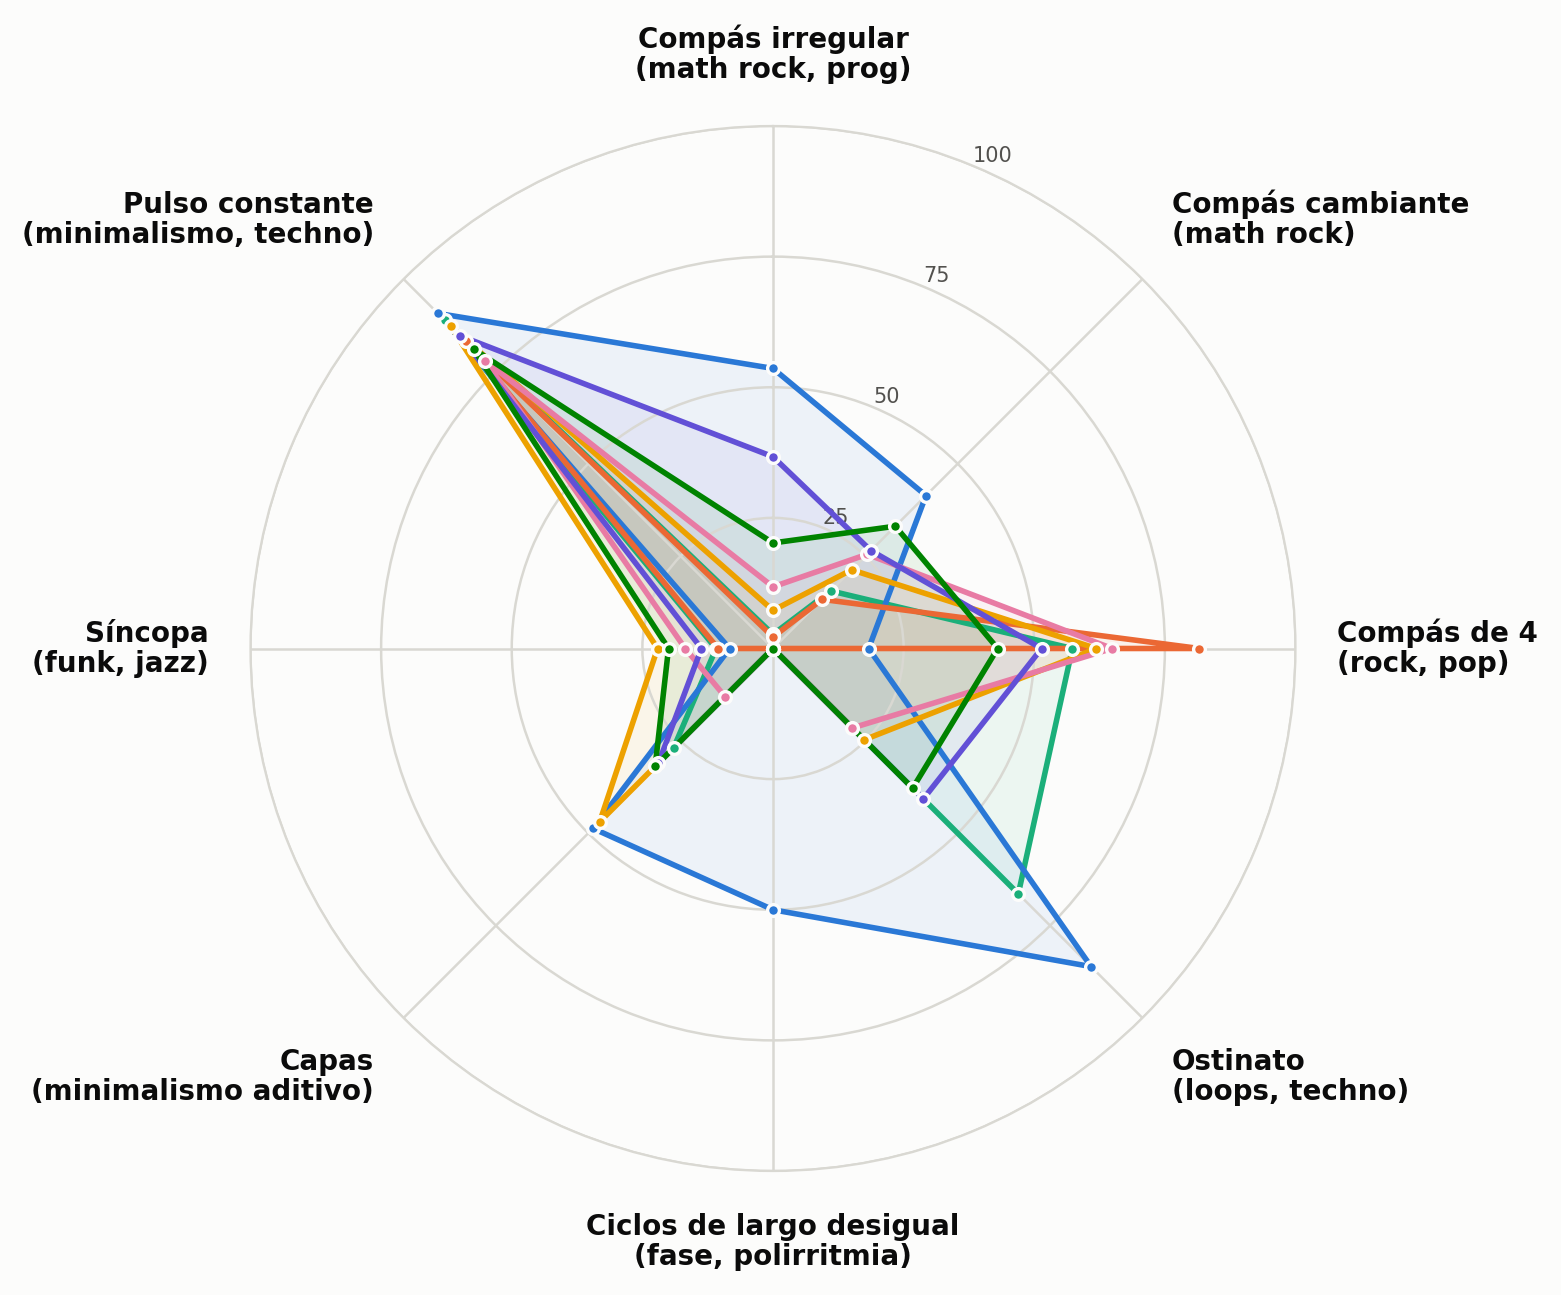
\includegraphics[width=0.55\textwidth]{g_radar_ritmico.png}
  \caption{Perfil rítmico por grupo (mediana, 0--100; más lejos del centro, más presente el rasgo). Verde azulado: la banda (5 canciones); azul: Fabienk, aparte; naranja: Primus; amarillo: King Gizzard; rosa: Zappa; violeta: King Crimson; verde: Gentle Giant.}\label{fig:radar-ritmico}
\end{figure}

\subsection{Bucle contra compás}

El compás que lee la herramienta y el ciclo del riff no siempre coinciden. Para cada compás se busca en qué punto del bucle
cae su primer tiempo (la rotación de la plantilla del bucle que mejor encaja con lo que suena). Si el compás mide lo mismo
que el bucle o lo divide, esa fase queda fija; si mide otra cosa, la fase avanza en escalera, compás a compás; un salto
aislado tras un silencio indica que el riff volvió a entrar por otro punto (figura~\ref{fig:bucle}).

\begin{figure}[htbp]
  \centering
  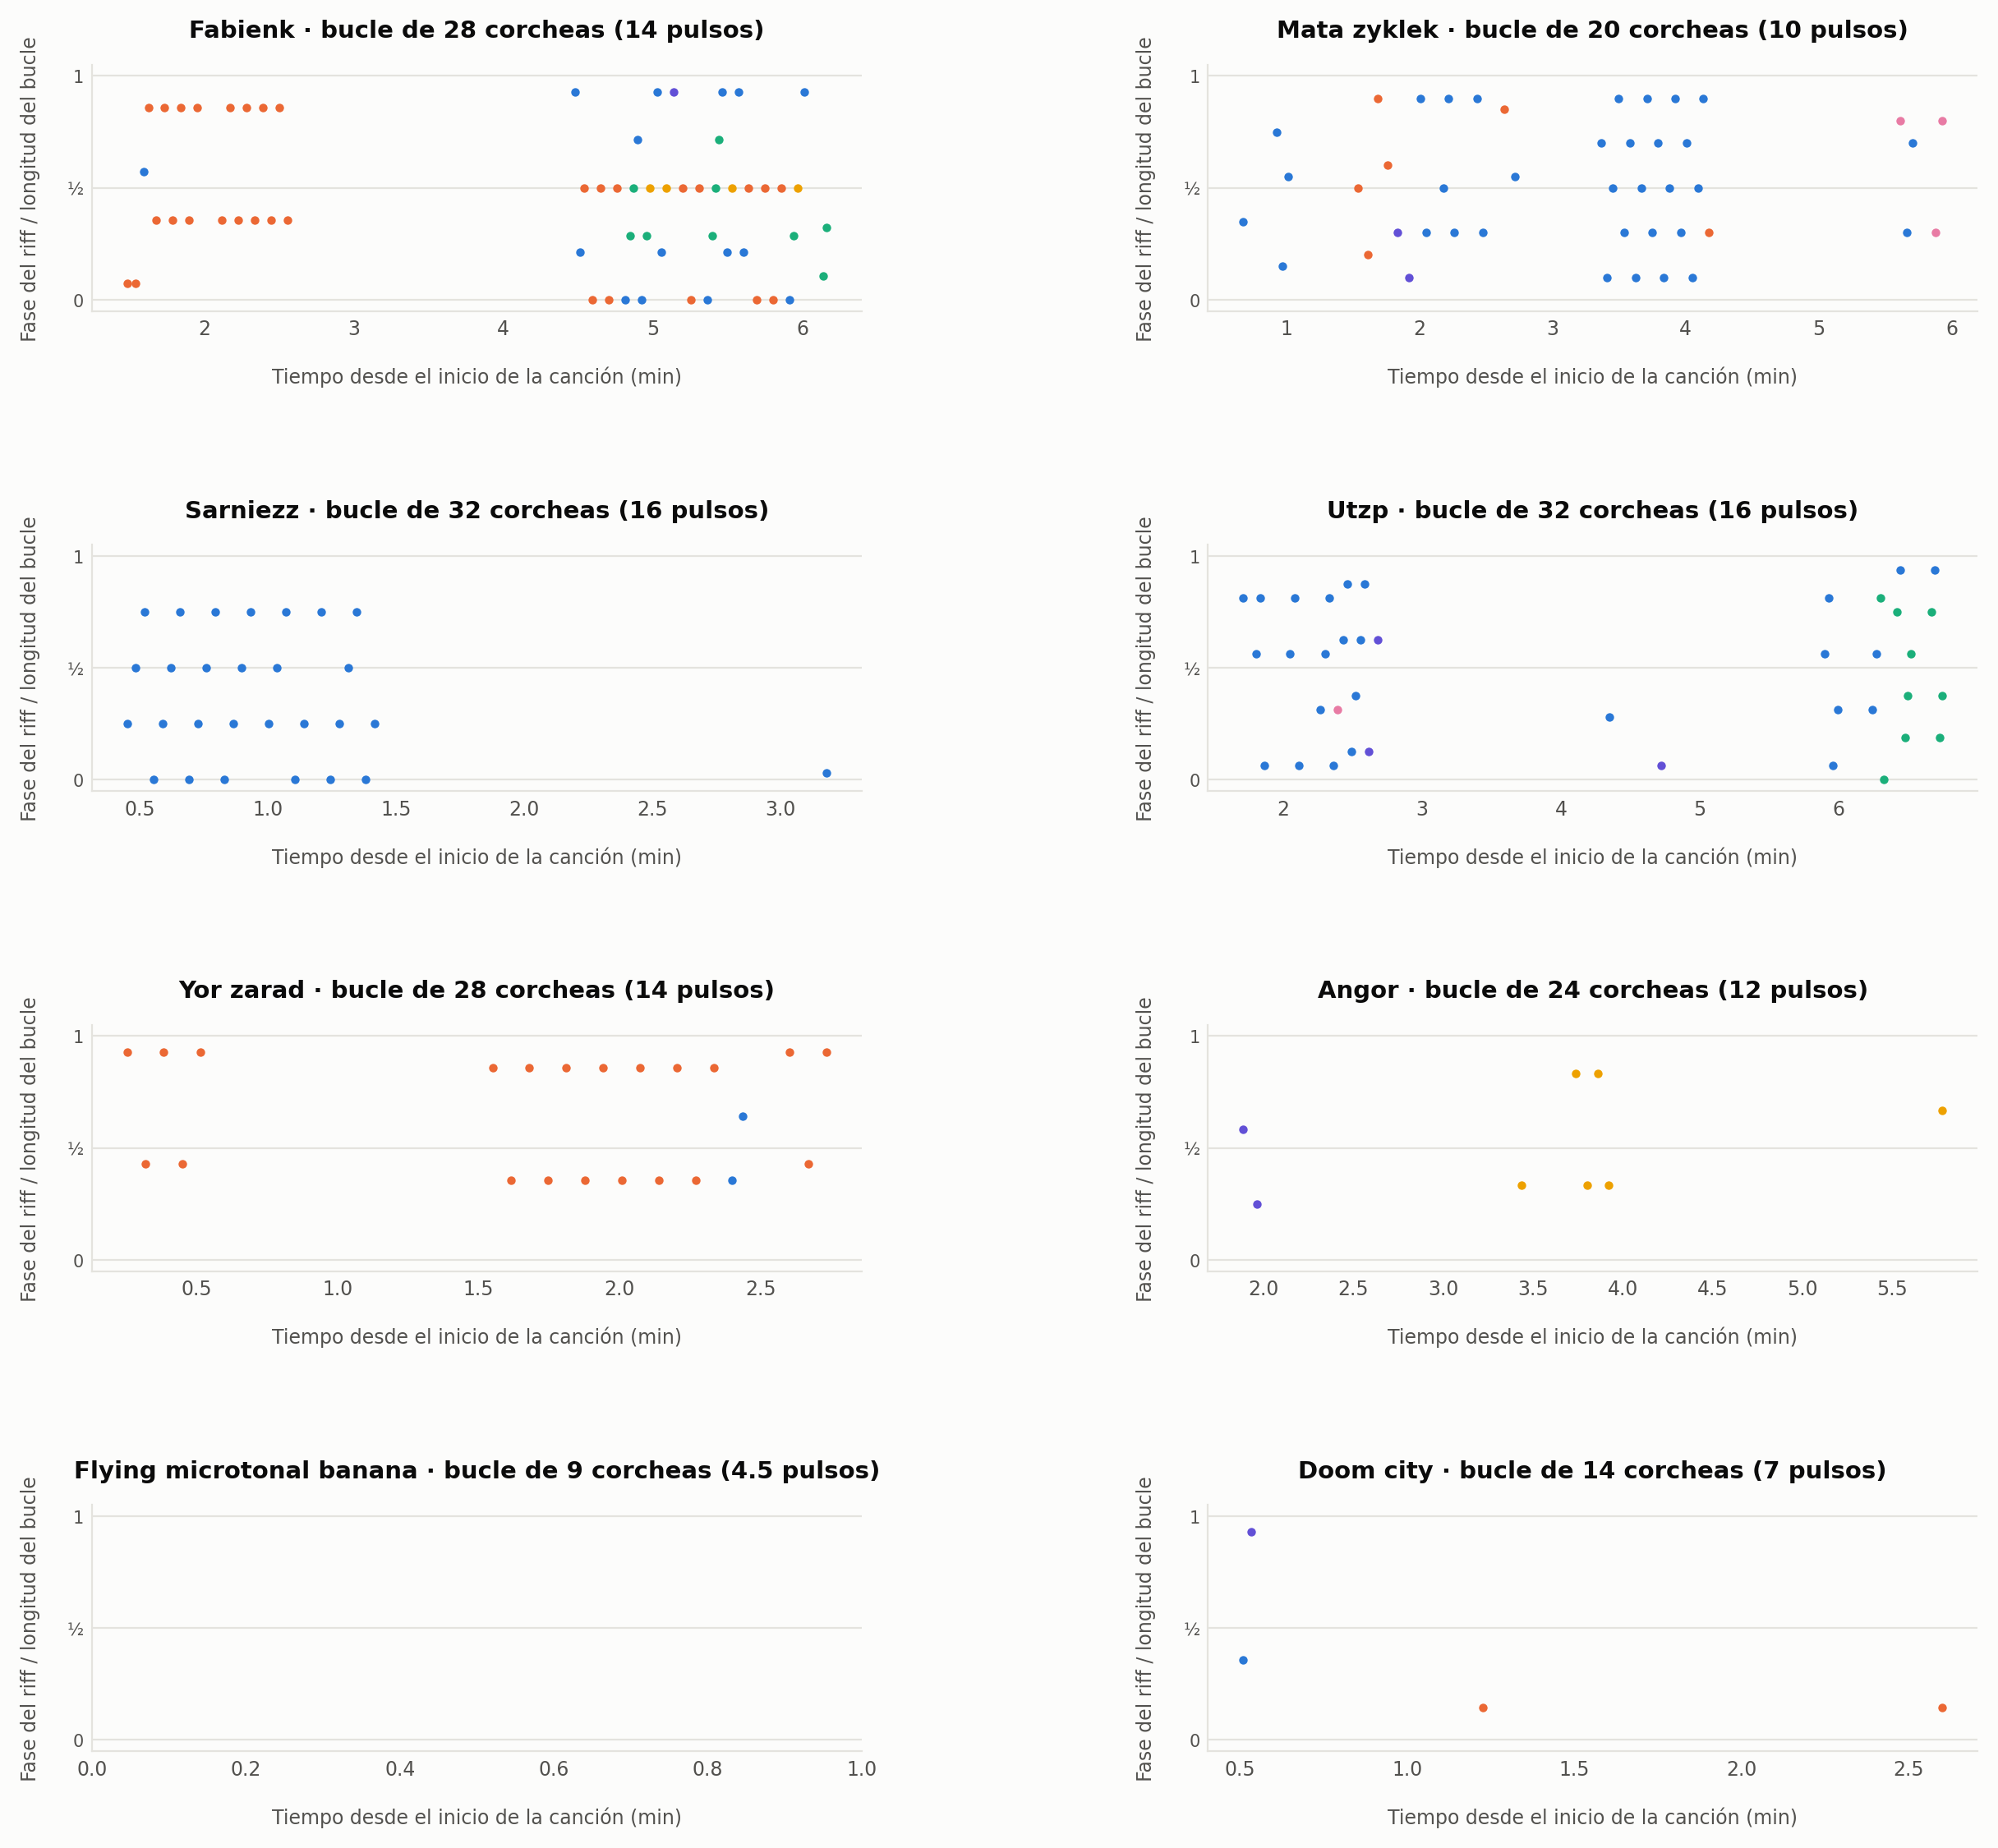
\includegraphics[width=0.92\textwidth]{bucle_compas.png}
  \caption{Fase del riff al inicio de cada compás: cada punto es un compás (eje $x$: minuto; eje $y$: fracción del bucle). Fase fija: compás y bucle coinciden; en escalera: tienen largos distintos; salto aislado: el riff vuelve a entrar tras un silencio. Color: pulsos del compás (verde 3, azul 4, rosa 5, amarillo 6, naranja 7, violeta 8). Las dos últimas son de King Gizzard; en «Flying Microtonal Banana» no queda ningún compás que graficar.}\label{fig:bucle}
\end{figure}

\begin{table}[ht]
  \centering\small
  \caption{Bucle contra compás: fracción de compases que no dividen al bucle ni son múltiplo de él.}\label{tab:bucle}
  \begin{tabular}{@{}lrr@{}}
    \toprule
    Canción & Bucle (corcheas) & Compases que no encajan \\
    \midrule
    Mata Zyklek & 20 & 93\,\% \\
    Fabienk & 28 & 48\,\% \\
    Utzp & 32 & 26\,\% \\
    Angor & 24 & 25\,\% \\
    Yor Zarad & 28 & 9\,\% \\
    Sarniezz & 32 & 0\,\% \\
    \bottomrule
  \end{tabular}
\end{table}

La tabla~\ref{tab:bucle} cuenta, en cada canción, los compases que no encajan. En Mata Zyklek, el 93\,\% no encaja con
el bucle: la herramienta lee la mayor parte de la canción en 4
(compases de 8 corcheas), mientras que el riff dura 20 corcheas. En todos los pasos de un compás al siguiente la fase
avanza exactamente lo que mide el compás, sin saltos: es una escalera regular, como la que produciría un polímetro, un
riff de 5 sobre un pulso de 4, tal como propone Mathémusique \citep{mathemusique2026}. La otra explicación es que la
herramienta lea mal el compás. Los datos no permiten decidir entre las dos, y queda como pregunta para comprobar de oído.
En Sarniezz, en cambio, compás y bucle encajan siempre: todo va en 4.

\section{Síntesis: un híbrido}\label{sec:res-sintesis}

La figura~\ref{fig:clasificacion} reúne los cuatro bloques. Los números de cada casilla muestran de dónde sale el color:
por ejemplo, Sarniezz da 34 en rock solo por el metro, porque su armonía da 0. El 83 de Mata Zyklek en práctica común no
es un parecido real: Kostka-Payne tiene solo 46 piezas y solo armonía, y la armonía de Mata Zyklek es un pedal (89\,\% del
tiempo sobre I y 6\,\% sobre V), un reparto tónica-dominante que tiene cualquier corpus tonal.

\begin{figure}[htbp]
  \centering
  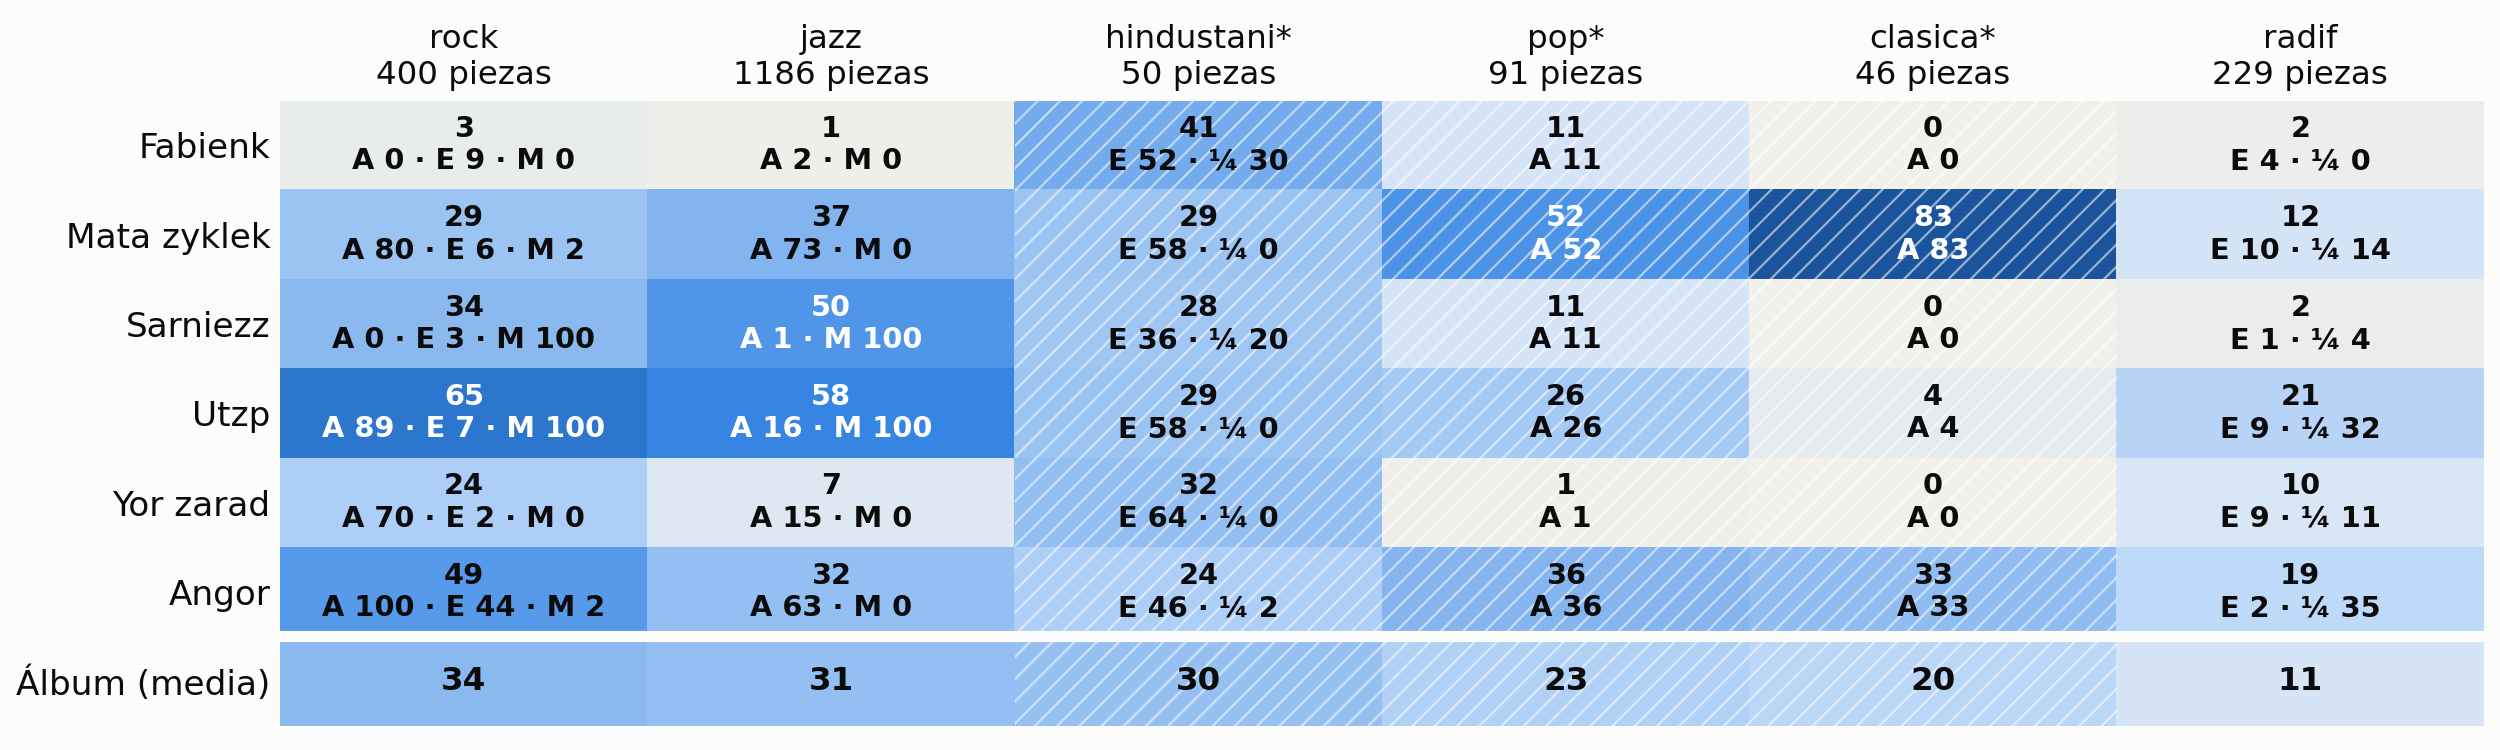
\includegraphics[width=\textwidth]{g_clasificacion_detalle.png}
  \caption{Clasificación del álbum por corpus. Color: percentil medio de tipicidad, de blanco (atípica) a azul oscuro (muy típica). En cada casilla, la media y el percentil de cada bloque (A armonía, E escala, \cuarto{} cuartos de tono, M metro). Asterisco y rayado: corpus de menos de 100 piezas, fuera del veredicto. En los encabezados, «clasica» es la práctica común y «hindustani», el corpus indostánico.}\label{fig:clasificacion}
\end{figure}

Las mismas medidas para las 36 canciones, bloque por bloque, están en el apéndice (figuras~\ref{fig:g-bloques}
y~\ref{fig:g-bloques-sintesis}).

Si se cuenta qué corpus se parece más en cada bloque (figura~\ref{fig:ganadores}), el rock gana 8 de 24, la mitad de
ellos en armonía (4 de 6 canciones): es rock modal. El radif gana 7, sobre todo en cuartos de tono. En los 9 restantes ningún corpus llega al
percentil 5. La tabla~\ref{tab:veredictos} da el veredicto de cada canción.

\begin{figure}[htbp]
  \centering
  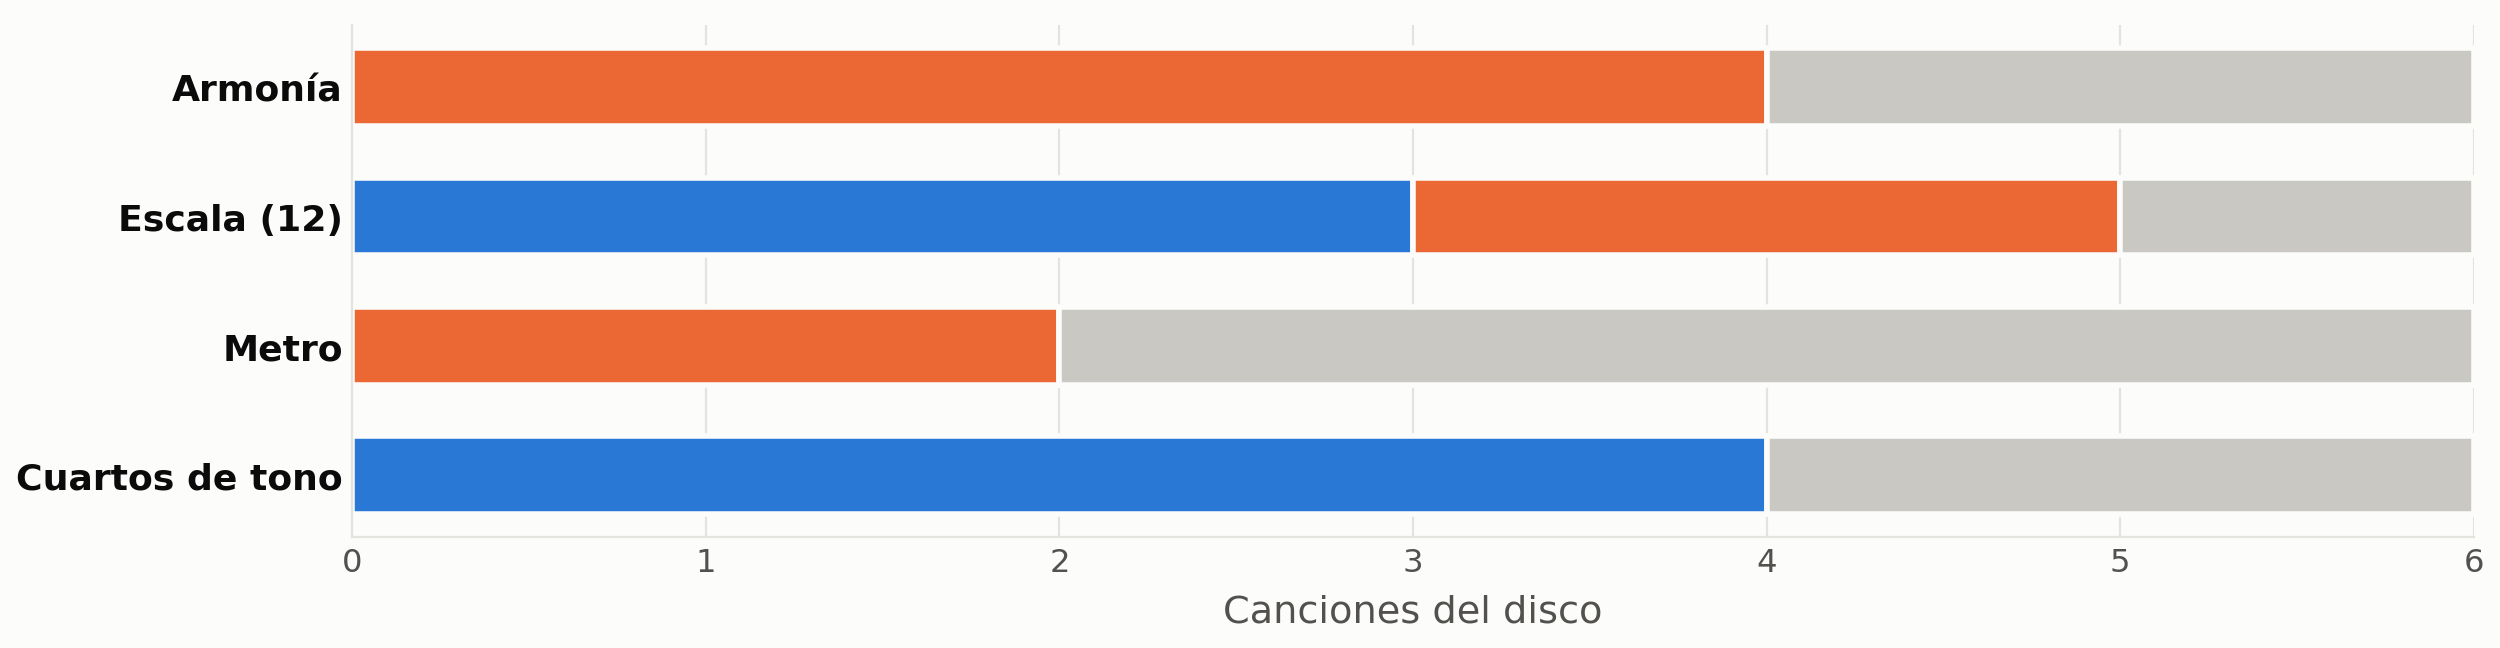
\includegraphics[width=0.85\textwidth]{3c_sintesis_corpus_por_bloque.png}
  \caption{Qué corpus gana cada bloque, en número de canciones. Azul: radif (7); naranja: rock (8); gris: sin vecino, ningún corpus llega al percentil 5 (9).}
  \label{fig:ganadores}
\end{figure}

\begin{table}[ht]
  \centering\small
  \caption{Veredicto del test por bloques (corpus con 100 piezas o más).}\label{tab:veredictos}
  \begin{tabularx}{\textwidth}{@{}l>{\raggedright\arraybackslash}X@{}}
    \toprule
    Canción & Veredicto \\
    \midrule
    Mata Zyklek & Rasgo sin vecino: metro \\
    Fabienk & Rasgo sin vecino: armonía, cuartos de tono y metro \\
    Sarniezz & Rasgo sin vecino: armonía, escala y cuartos de tono \\
    Yor Zarad & Rasgo sin vecino: metro \\
    Angor & Rasgo sin vecino: metro \\
    Utzp & Síntesis de lenguajes existentes \\
    \bottomrule
  \end{tabularx}
\end{table}

En ningún caso el veredicto es «estilo existente»: ningún corpus tiene los cuatro bloques, y ninguno explica la
combinación. El vecino más cercano en conjunto es King Gizzard: en armonía, Angor es idéntica a «Flying Microtonal
Banana», porque ambas son un pedal sobre I. Sarniezz y Fabienk no tienen vecino ni siquiera ahí.

\section{Análisis por canción}\label{sec:por-cancion}

Esta sección reúne, canción por canción, lo que la herramienta mide en el álbum. Para cada una se muestran una página del
tabroll con la armonía en 24-EDO y el mapa de ciclos del looper. En el tabroll, las filas son las 24 clases por octava
(las filas «¼» son los cuartos de tono), cada recuadro es un compás con su número de pulsos arriba y su acorde abajo
(cifrado romano, función y nombre; entre paréntesis, los compases de baja confianza), y los anillos dorados marcan la
columna principal del compás. En el mapa de ciclos, cada barra es un tramo en que una voz repite un ciclo, con su letra y
su periodo, y la curva inferior estima cuántas capas del looper suenan.

La tabla~\ref{tab:resumen-canciones} resume las medidas principales.

\begin{table}[ht]
  \centering\footnotesize\setlength{\tabcolsep}{4pt}
  \caption{Resumen por canción. «Conf.»: porcentaje del tiempo en compases confiables. «Ciclo»: mejor periodo de
  $R(\ell)$ en corcheas.}\label{tab:resumen-canciones}
  \begin{tabular}{@{}lrrlllrr@{}}
    \toprule
    Canción & BPM & Conf. & Centro & Modo (2, 3, 6, 7) & \shortstack{Fundamental\\más usada} & \shortstack{\cuarto{} de\\tono} & Ciclo \\
    \midrule
    Mata Zyklek & 94 & 78\,\% & Sol & \fl2+, 3, \fl6+, \fl7 & I (89\,\%) & 23.9\,\% & 20 \\
    Fabienk & 129 & 85\,\% & Mi & 2, \fl3, 6, \fl7 & I, \fl VII, \fl III & 14.2\,\% & 28 \\
    Sarniezz & 115 & 58\,\% & Mi & 2, \fl3, 6, \fl7 & \fl III (40\,\%) & 25.3\,\% & 32 \\
    Yor Zarad & 108 & 75\,\% & Sol & \fl2+, 3, \fl6+, \fl7 & I (85\,\%) & 16.8\,\% & 28 \\
    Utzp & 129 & 82\,\% & Mi & \fl2+, \fl3, \fl6+, \fl7 & I (96\,\%) & 11.1\,\% & 32 \\
    Angor & 99 & 88\,\% & Sol & \fl2+, \fl3, 6, \fl7 & I (100\,\%) & 5.0\,\% & 24 \\
    \bottomrule
  \end{tabular}
\end{table}

Los modos confirman las dos familias de la sección~\ref{sec:res-melodia}. Mata Zyklek y Yor Zarad tienen la misma
descripción: \fl2+, 3, \fl6+, \fl7. Es un frigio dominante (\fl2, 3, \fl6, \fl7) con la segunda y la sexta subidas un
cuarto de tono, es decir, con una segunda neutra en lugar de la aumentada; en doce notas se leería como hijaz, y eso
explica la comparación de David Bennett. Utzp es el mismo esquema sobre un frigio menor (\fl3). Fabienk y Sarniezz son
dóricos (2, \fl3, 6, \fl7), con los cuartos de tono en la melodía (7+, 6+, \fl3+) y no en el modo de los acordes.

\FloatBarrier
\subsection{Mata Zyklek}

La figura~\ref{fig:mata} muestra una página del tabroll24 y el mapa de ciclos; la tarjeta y la tira de ciclos son las figuras~\ref{fig:tarjeta-mata} y~\ref{fig:tira-mata}, y su círculo armónico está en el apéndice (figura~\ref{fig:circulos1}).

\begin{figure}[p]
  \centering
  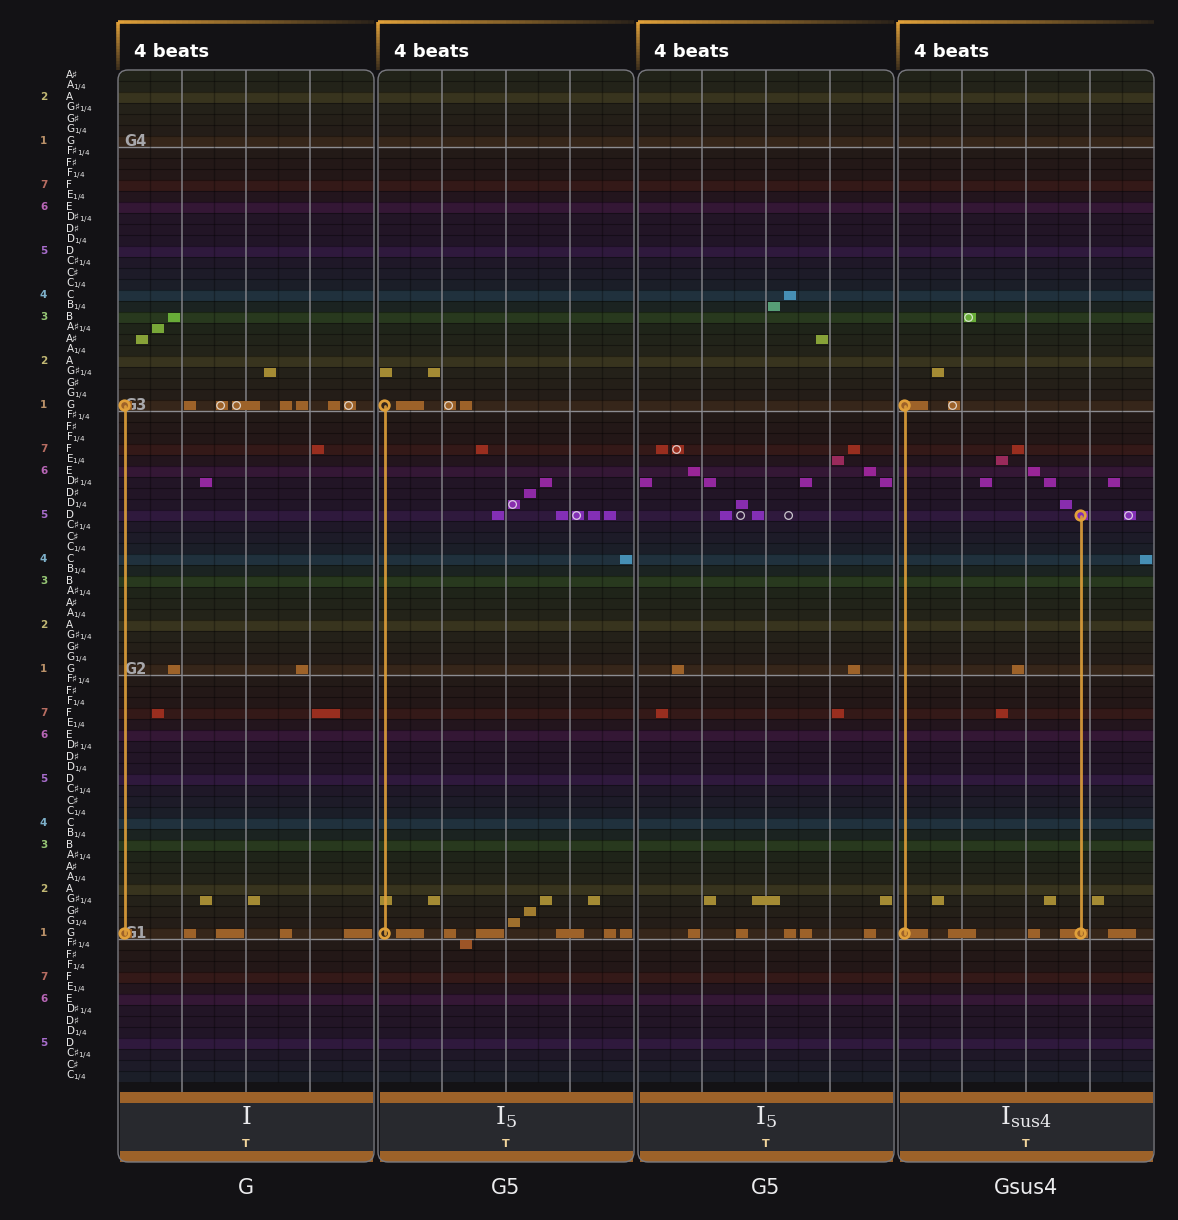
\includegraphics[width=0.78\textwidth]{mata_zyklek_tabroll24.png}\\[0.5em]
  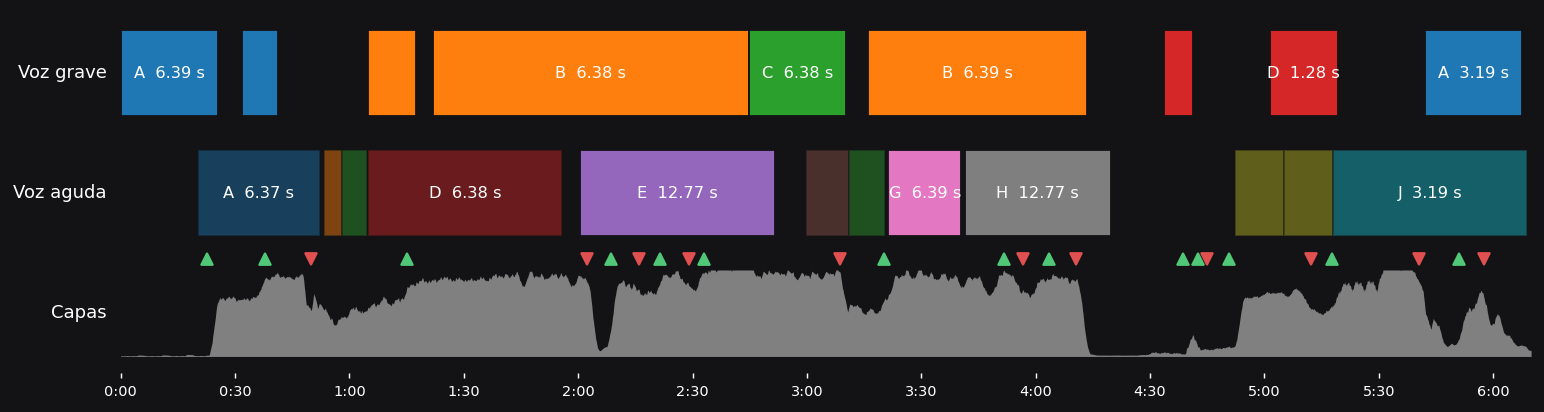
\includegraphics[width=\textwidth]{mata_zyklek_mapa_ciclos.png}
  \caption{Mata Zyklek. Arriba, una página del tabroll24: notas en 24-EDO (filas «¼», cuartos de tono), pulsos de cada compás («beats») y acorde debajo. Abajo, mapa de ciclos: cada barra es un tramo repetido de una voz, con su letra y su periodo; la curva gris estima las capas del looper (triángulos verdes: entra una capa; rojos: sale).}\label{fig:mata}
\end{figure}

\paragraph{Armonía.} Es un pedal: la fundamental está en I el 89\,\% del tiempo (quinta sola el 53\,\% y tríada mayor el
34\,\%), con V (6\,\%), \fl2+ (3\,\%) y \fl VII (2\,\%). Entre compases confiables solo hay dos cambios, I5 $\to$ Vsus4
$\to$ I: una cadencia auténtica. Con todos los compases aparece además, en la introducción, el vaivén \fl II+5
$\leftrightarrow$ \fl VII, que la partitura confirma pero que tiene confianza baja (0.14 a 0.44). La introducción está
centrada en Sol\sh+ (\fl2+): la canción empieza sobre el cuarto de tono y llega a Sol.

\paragraph{Melodía.} Es la canción con más tiempo en cuartos de tono como grado (19.1\,\%). Los dos grados principales son
\fl2+ (11.3\,\% del tiempo de la melodía) y \fl6+ (5.2\,\%); \fl2+ y 1+ aparecen en todas las vueltas del ciclo. En el bajo,
lo que más varía entre vueltas es Sol\sh+ $\leftrightarrow$ Sol: la fundamental y su segunda neutra (\fl2+), tres cuartos de tono más arriba.

\paragraph{Metro y comparación.} El riff se repite cada 20 corcheas (dos compases de 5/4, $R = 0.82$). En el test por bloques
su armonía tiene vecinos en el rock (percentil 79.5): el rock tiene piezas de pedal, aunque frente al \emph{centro} del rock
quede lejos (12 en la matriz). Lo que no tiene vecino es el metro.

\FloatBarrier
\subsection{Fabienk}

La figura~\ref{fig:fabienk-tarjeta} reúne la tarjeta y la tira de ciclos; la figura~\ref{fig:fabienk}, una página del tabroll24 y el mapa de ciclos.

\begin{figure}[!h]
  \centering
  \begin{subfigure}[c]{0.42\textwidth}\centering
    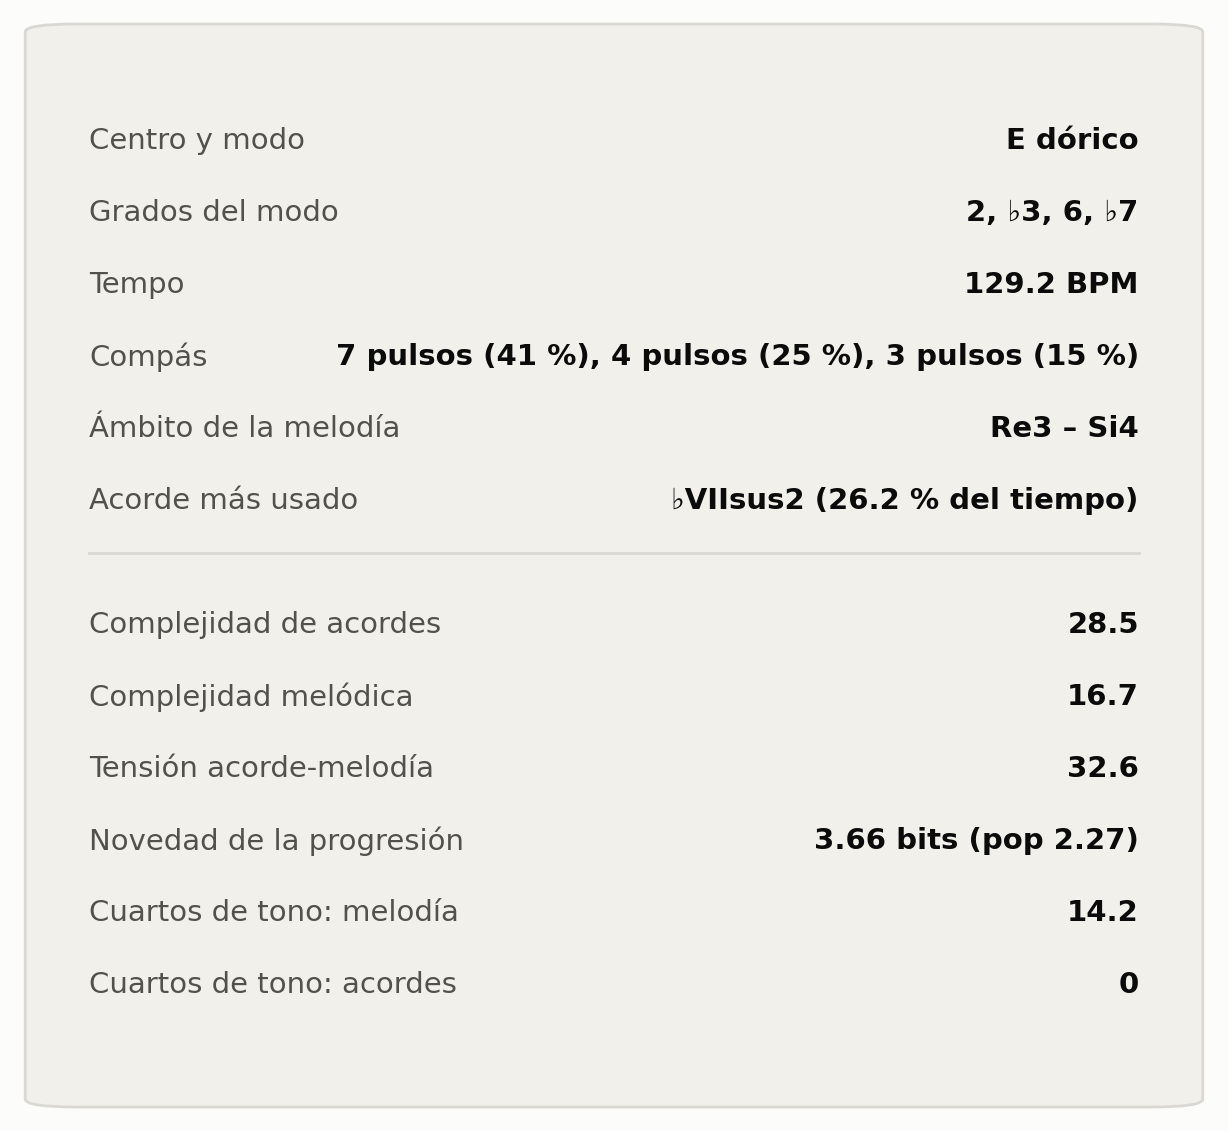
\includegraphics[width=\linewidth]{fabienk_tarjeta.png}\caption{Tarjeta.}
  \end{subfigure}\hfill
  \begin{subfigure}[c]{0.55\textwidth}\centering
    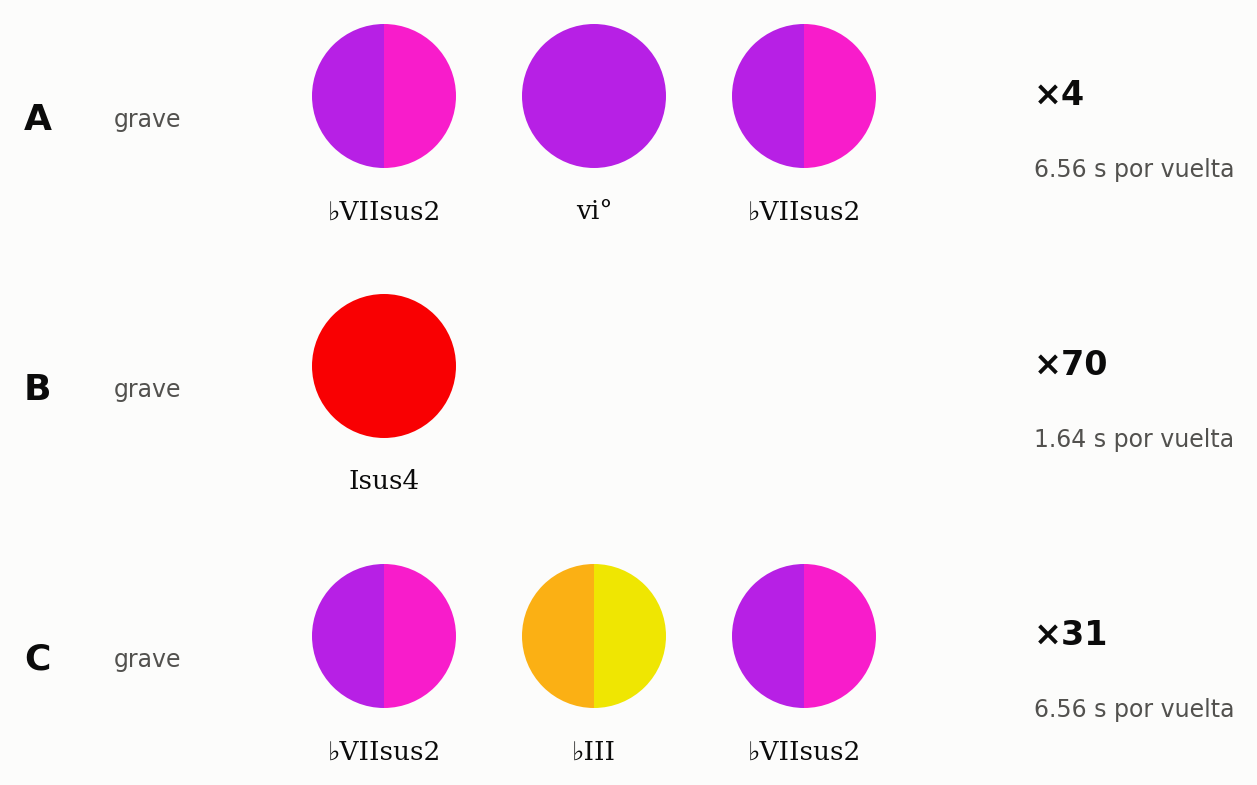
\includegraphics[width=\linewidth]{fabienk_tira_de_ciclos.png}\caption{Ciclos repetidos.}
  \end{subfigure}
  \caption{Fabienk: tarjeta de medidas crudas (izquierda) y tira de ciclos (derecha; cada fila es un ciclo de la voz indicada, grave o aguda; color = grado de la fundamental, $\times$ = vueltas, s = duración de cada vuelta). Centro Mi, modo 2, \fl3, 6, \fl7; compases confiables: 84.7\,\%; acierto F 45.4 en la melodía y 81.6 en la fundamental.}\label{fig:fabienk-tarjeta}
\end{figure}

\begin{figure}[p]
  \centering
  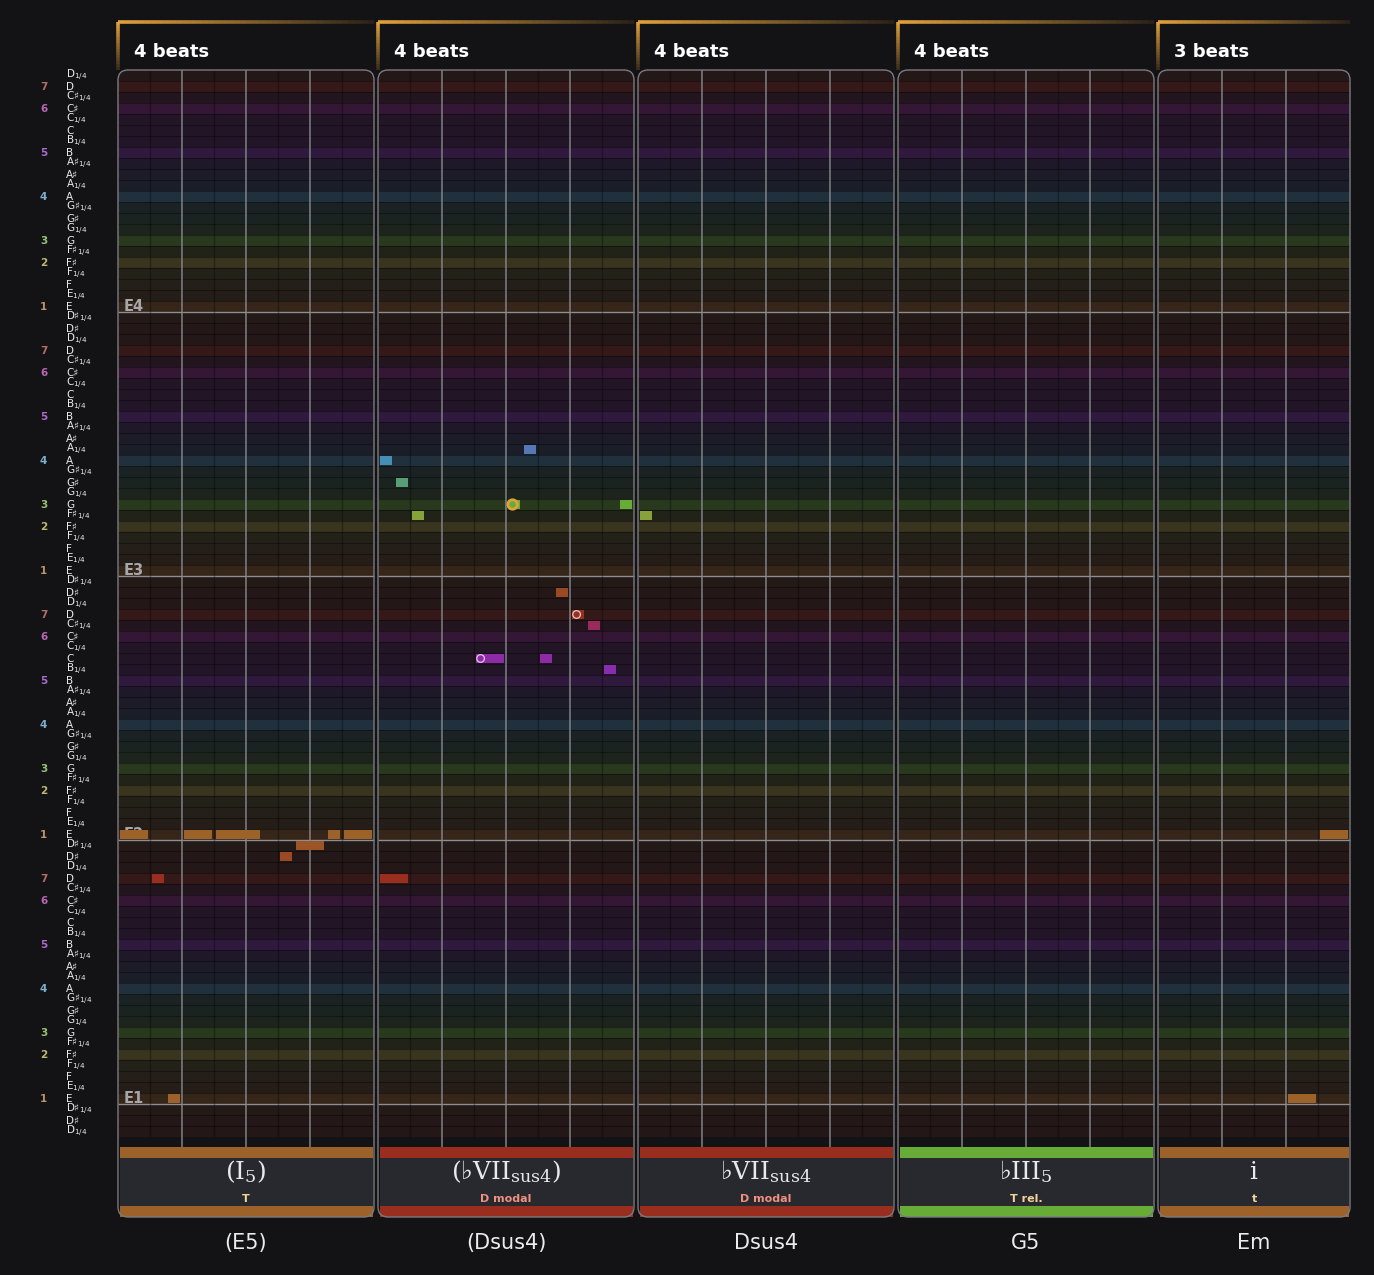
\includegraphics[width=0.7\textwidth]{fabienk_tabroll24.png}\\[0.5em]
  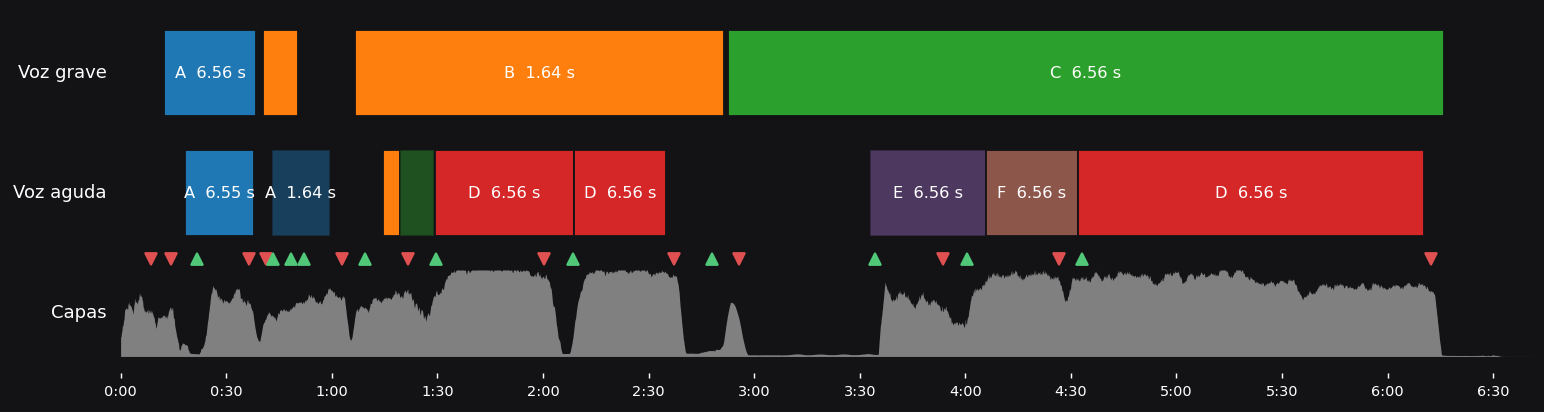
\includegraphics[width=\textwidth]{fabienk_mapa_ciclos.png}
  \caption{Fabienk: una página del tabroll24 (arriba) y el mapa de ciclos (abajo); misma lectura que la figura~\ref{fig:mata}.}\label{fig:fabienk}
\end{figure}

\paragraph{Armonía.} Es la canción con más movimiento armónico: 86 cambios entre compases confiables, la mitad por quintas
(51\,\%), seguidos de segundas (28\,\%) y terceras abajo (21\,\%). Tres fundamentales se reparten el tiempo casi por igual:
I (34\,\%), \fl VII (33\,\%) y \fl III (29\,\%). Las progresiones más frecuentes son \fl VII $\to$ \fl III y el vaivén
\fl III $\leftrightarrow$ \fl VIIsus2; aparece la cadencia modal \fl VII--I. El acorde más usado es \fl VIIsus2 (26\,\%).
El centro es dudoso (margen 0.015): el bajo descansa en \fl VII, y por eso se usa el centro que coincide con el oído, Mi.

\paragraph{Melodía.} Los cuartos de tono ocupan el 14.2\,\% de la melodía, concentrados en 7+ (4.6\,\%) y 6+ (4.3\,\%); 6+
aparece en todas las vueltas del ciclo.

\paragraph{Metro.} El ciclo dura 28 corcheas, dos compases de 7/4 ($R = 0.87$, empatado con Utzp como el más estable del álbum). La canción pasa
el 53\,\% del tiempo en compases de 7, el 18\,\% en 4 y el 9\,\% en 3. La tarjeta de la figura~\ref{fig:fabienk-tarjeta}
cuenta compases y no tiempo: 41\,\% de 7, 25\,\% de 4 y 15\,\% de 3; como el compás de 7 es el más largo, pesa más en
tiempo que en número. Sin vecino en armonía, cuartos de tono y metro.

\clearpage
\subsection{Sarniezz}

La figura~\ref{fig:sarniezz-tarjeta} reúne la tarjeta y la tira de ciclos; la figura~\ref{fig:sarniezz}, una página del tabroll24 y el mapa de ciclos.

\begin{figure}[!h]
  \centering
  \begin{subfigure}[c]{0.42\textwidth}\centering
    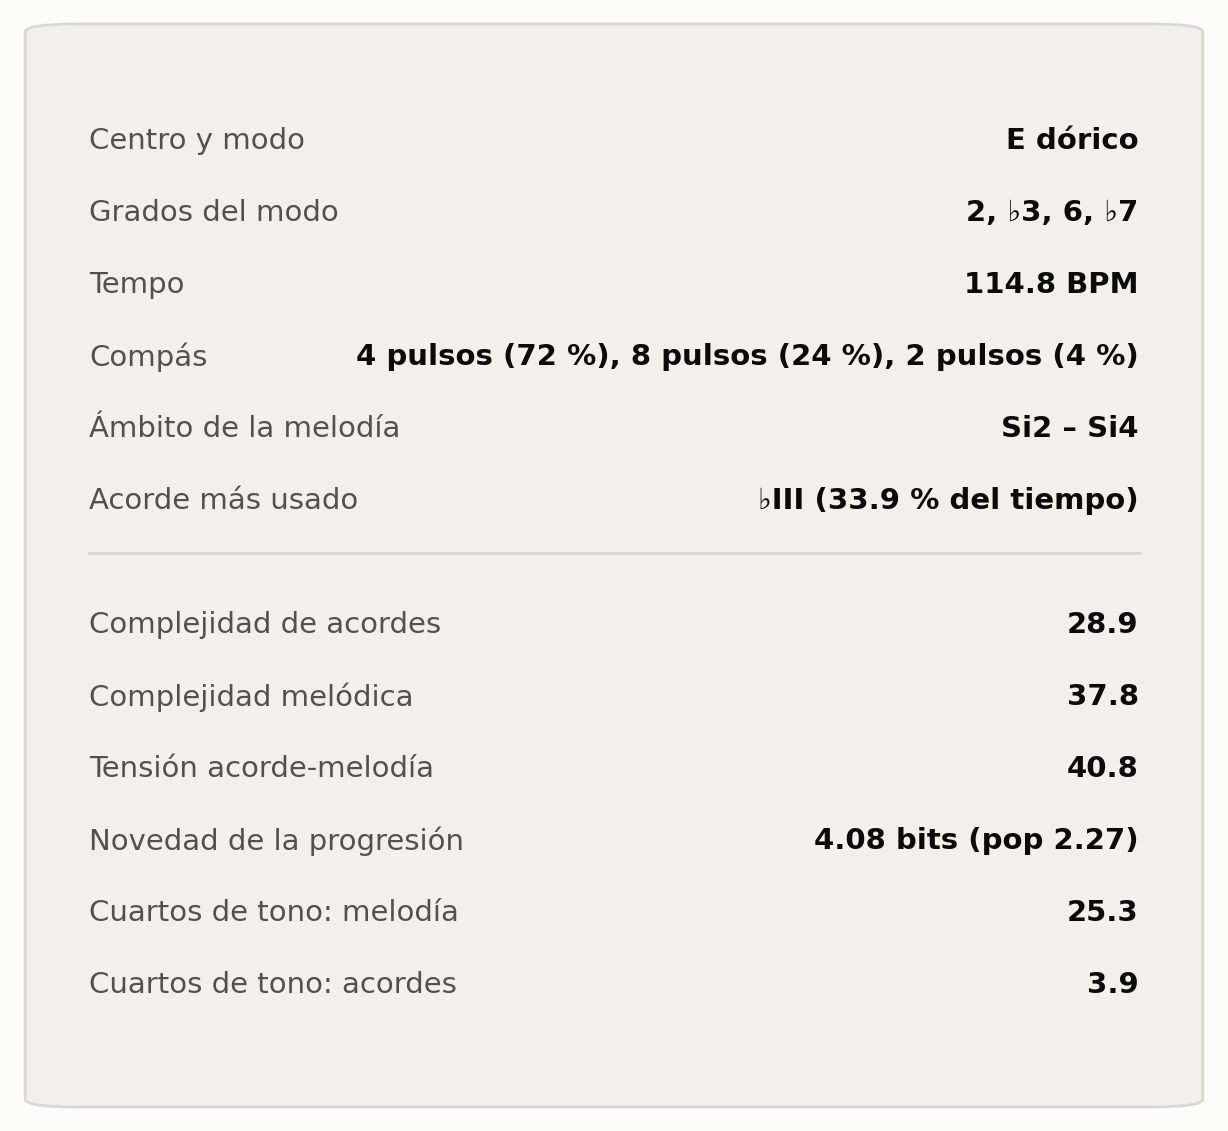
\includegraphics[width=\linewidth]{sarniezz_tarjeta.png}\caption{Tarjeta.}
  \end{subfigure}\hfill
  \begin{subfigure}[c]{0.55\textwidth}\centering
    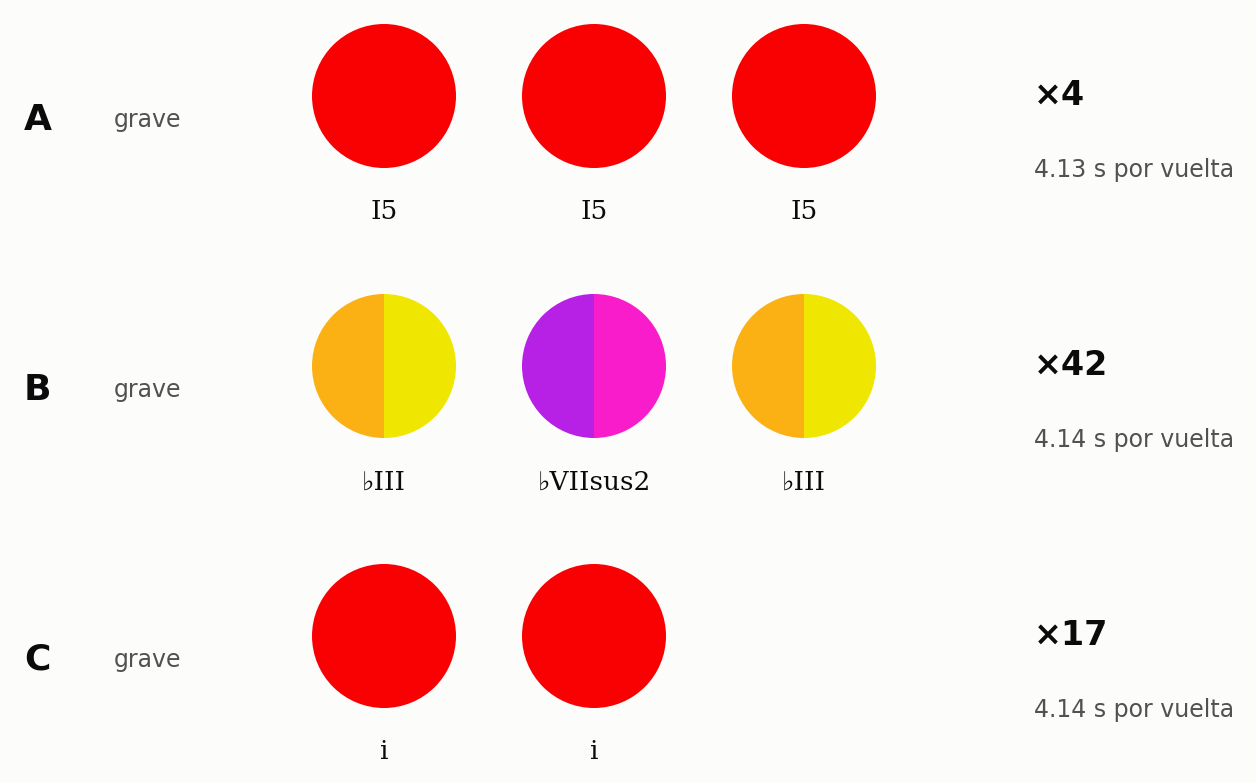
\includegraphics[width=\linewidth]{sarniezz_tira_de_ciclos.png}\caption{Ciclos repetidos.}
  \end{subfigure}
  \caption{Sarniezz: tarjeta y tira de ciclos; misma lectura que la figura~\ref{fig:fabienk-tarjeta}. Centro Mi, modo 2, \fl3, 6, \fl7; compases confiables: 57.6\,\%; acierto F 44.9 en la melodía y 57.5 en la fundamental.}\label{fig:sarniezz-tarjeta}
\end{figure}

\begin{figure}[p]
  \centering
  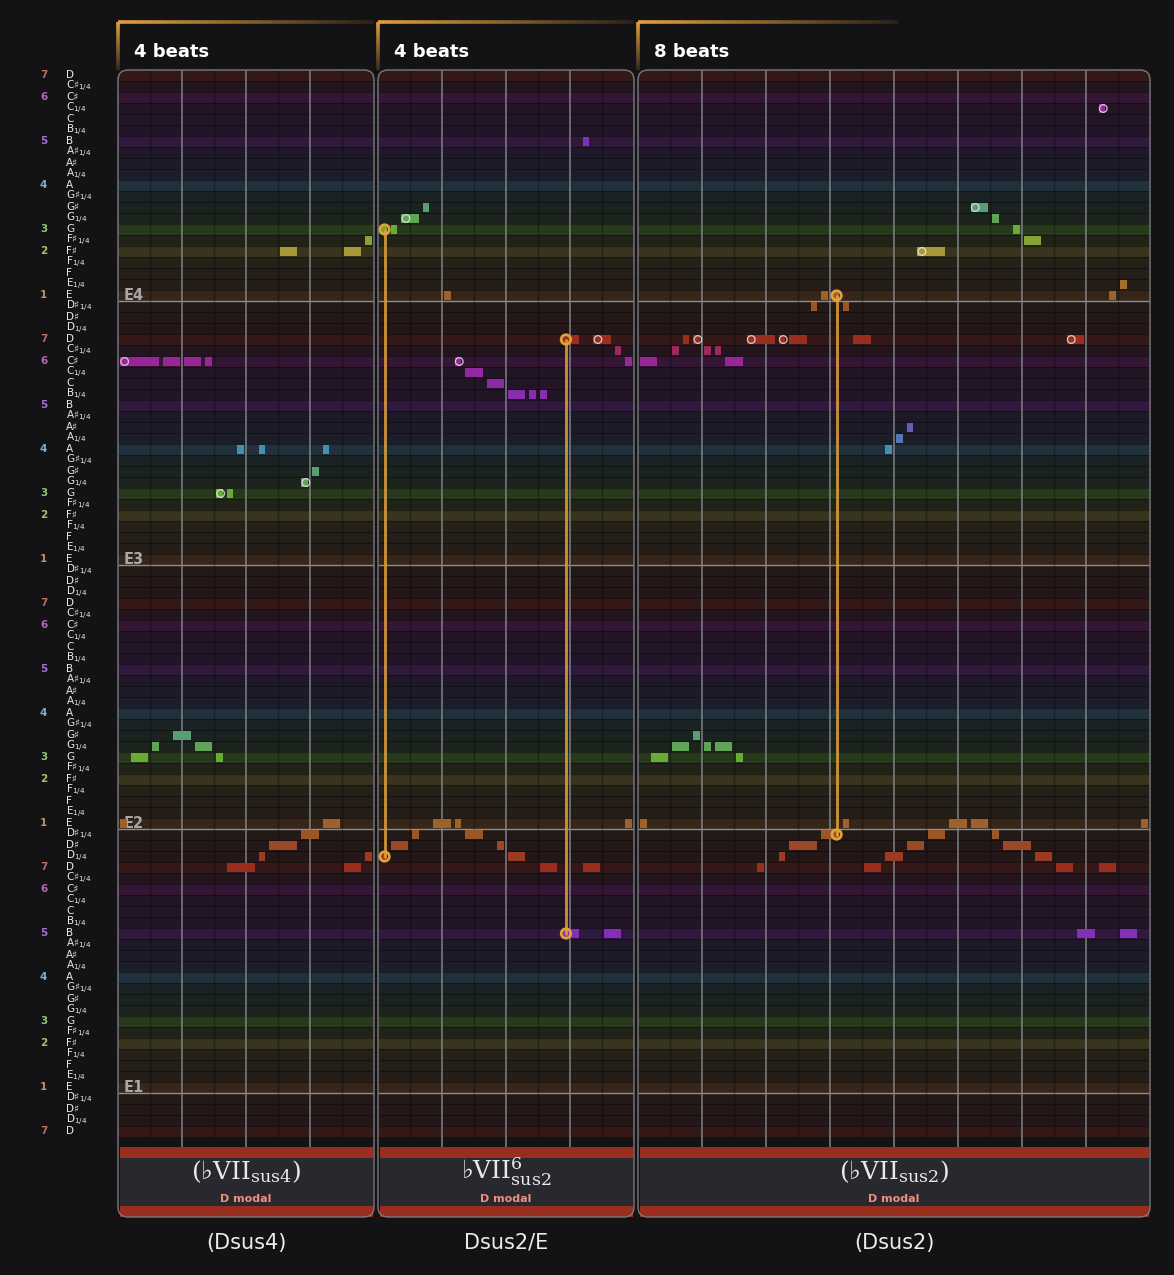
\includegraphics[width=0.7\textwidth]{sarniezz_tabroll24.png}\\[0.5em]
  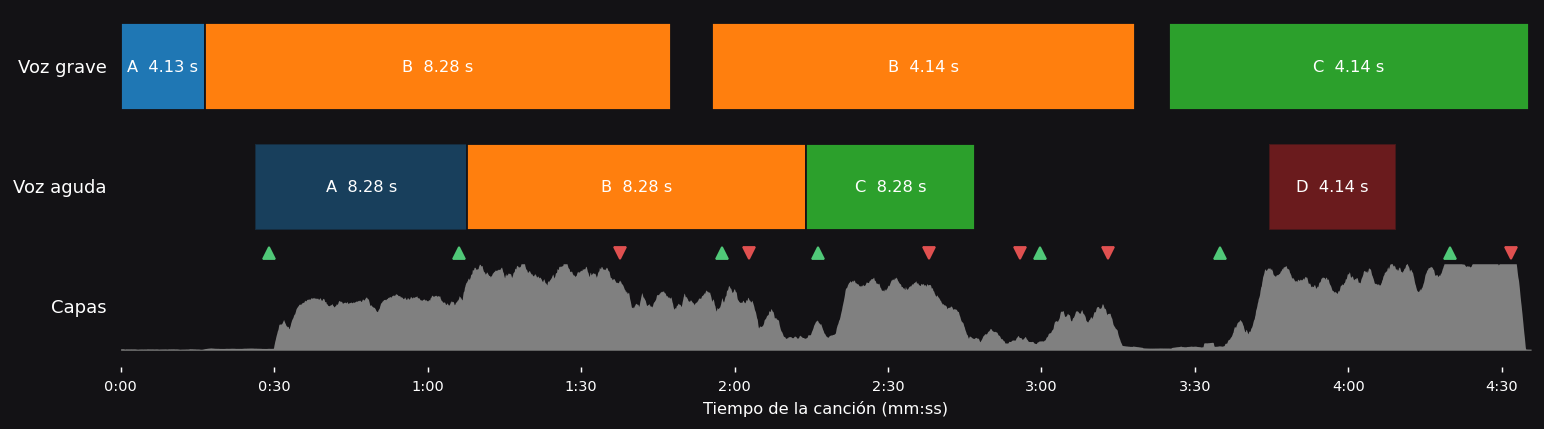
\includegraphics[width=\textwidth]{sarniezz_mapa_ciclos.png}
  \caption{Sarniezz: una página del tabroll24 (arriba) y el mapa de ciclos (abajo); misma lectura que la figura~\ref{fig:mata}.}\label{fig:sarniezz}
\end{figure}

\paragraph{Armonía.} La fundamental más usada no es la tónica sino \fl III (40\,\%), seguida de \fl VII (29\,\%) y I
(24\,\%). El vaivén \fl III $\leftrightarrow$ \fl VIIsus2 se repite 31 veces. El 59\,\% de los cambios va por quintas, pero
el 9\,\% es microtonal. Según los ejes de Lendvai, el 24\,\% de los cambios de la partitura queda dentro del eje de tónica
(I $\leftrightarrow$ \fl III), una sustitución y no un movimiento por quintas. Los centros por tramo muestran por qué el
centro es difícil: los tramos B giran sobre Re (\fl7) y el C sobre Sol (\fl3), y Mi solo ocupa el 6\,\% de los tramos. Es
la canción con menos compases confiables (58\,\%) y con la armonía menos acertada (57.5\,\%).

\paragraph{Melodía.} Tiene la mayor proporción de cuartos de tono (25.3\,\%) pero la menor concentración (48\,\%):
7+ (6.4\,\%), \fl3+ (5.9\,\%), \fl7+ (3.5\,\%) y 5+ (2.9\,\%). \fl3+ aparece en todas las vueltas y 7+ y 5+ en el 88\,\%.
Es un riff cromático de cuartos de tono, no una escala con dos grados neutros.

\paragraph{Metro.} Va en 4: el ciclo dura 32 corcheas. Sin vecino en armonía, escala y cuartos de tono.

\clearpage
\subsection{Yor Zarad}

La figura~\ref{fig:yor_zarad-tarjeta} reúne la tarjeta y la tira de ciclos; la figura~\ref{fig:yor}, una página del tabroll24 y el mapa de ciclos.

\begin{figure}[!h]
  \centering
  \begin{subfigure}[c]{0.42\textwidth}\centering
    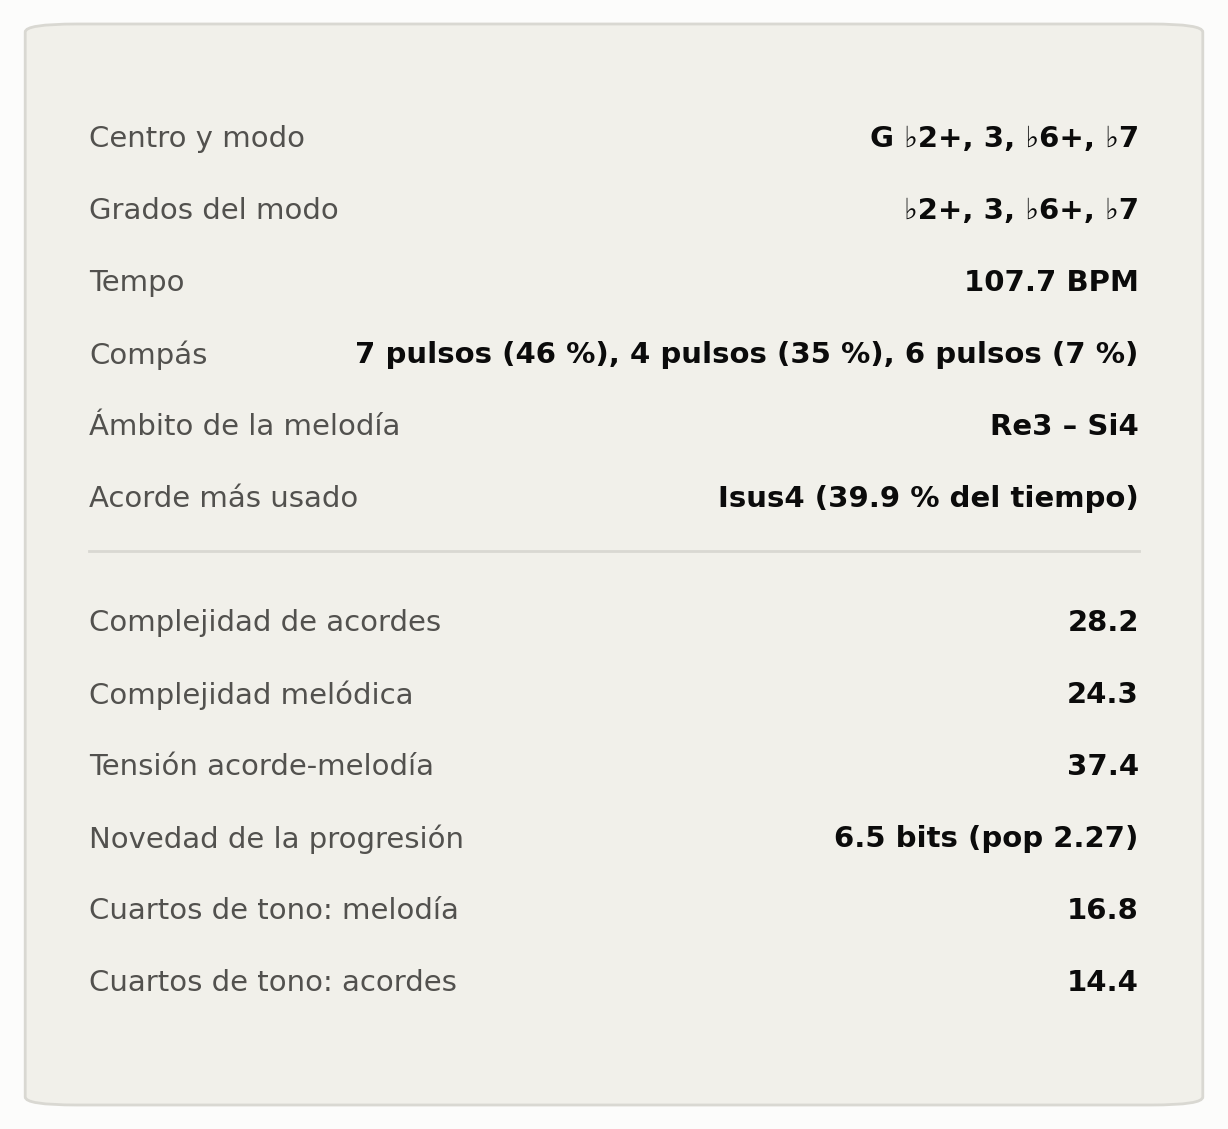
\includegraphics[width=\linewidth]{yor_zarad_tarjeta.png}\caption{Tarjeta.}
  \end{subfigure}\hfill
  \begin{subfigure}[c]{0.55\textwidth}\centering
    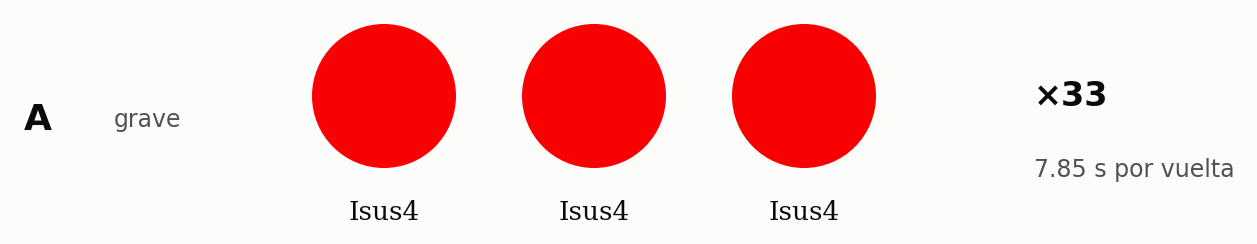
\includegraphics[width=\linewidth]{yor_zarad_tira_de_ciclos.png}\caption{Ciclos repetidos.}
  \end{subfigure}
  \caption{Yor Zarad: tarjeta y tira de ciclos; misma lectura que la figura~\ref{fig:fabienk-tarjeta}. Centro Sol, modo \fl2+, 3, \fl6+, \fl7; compases confiables: 75.2\,\%; acierto F 36.8 en la melodía.}\label{fig:yor_zarad-tarjeta}
\end{figure}

\begin{figure}[p]
  \centering
  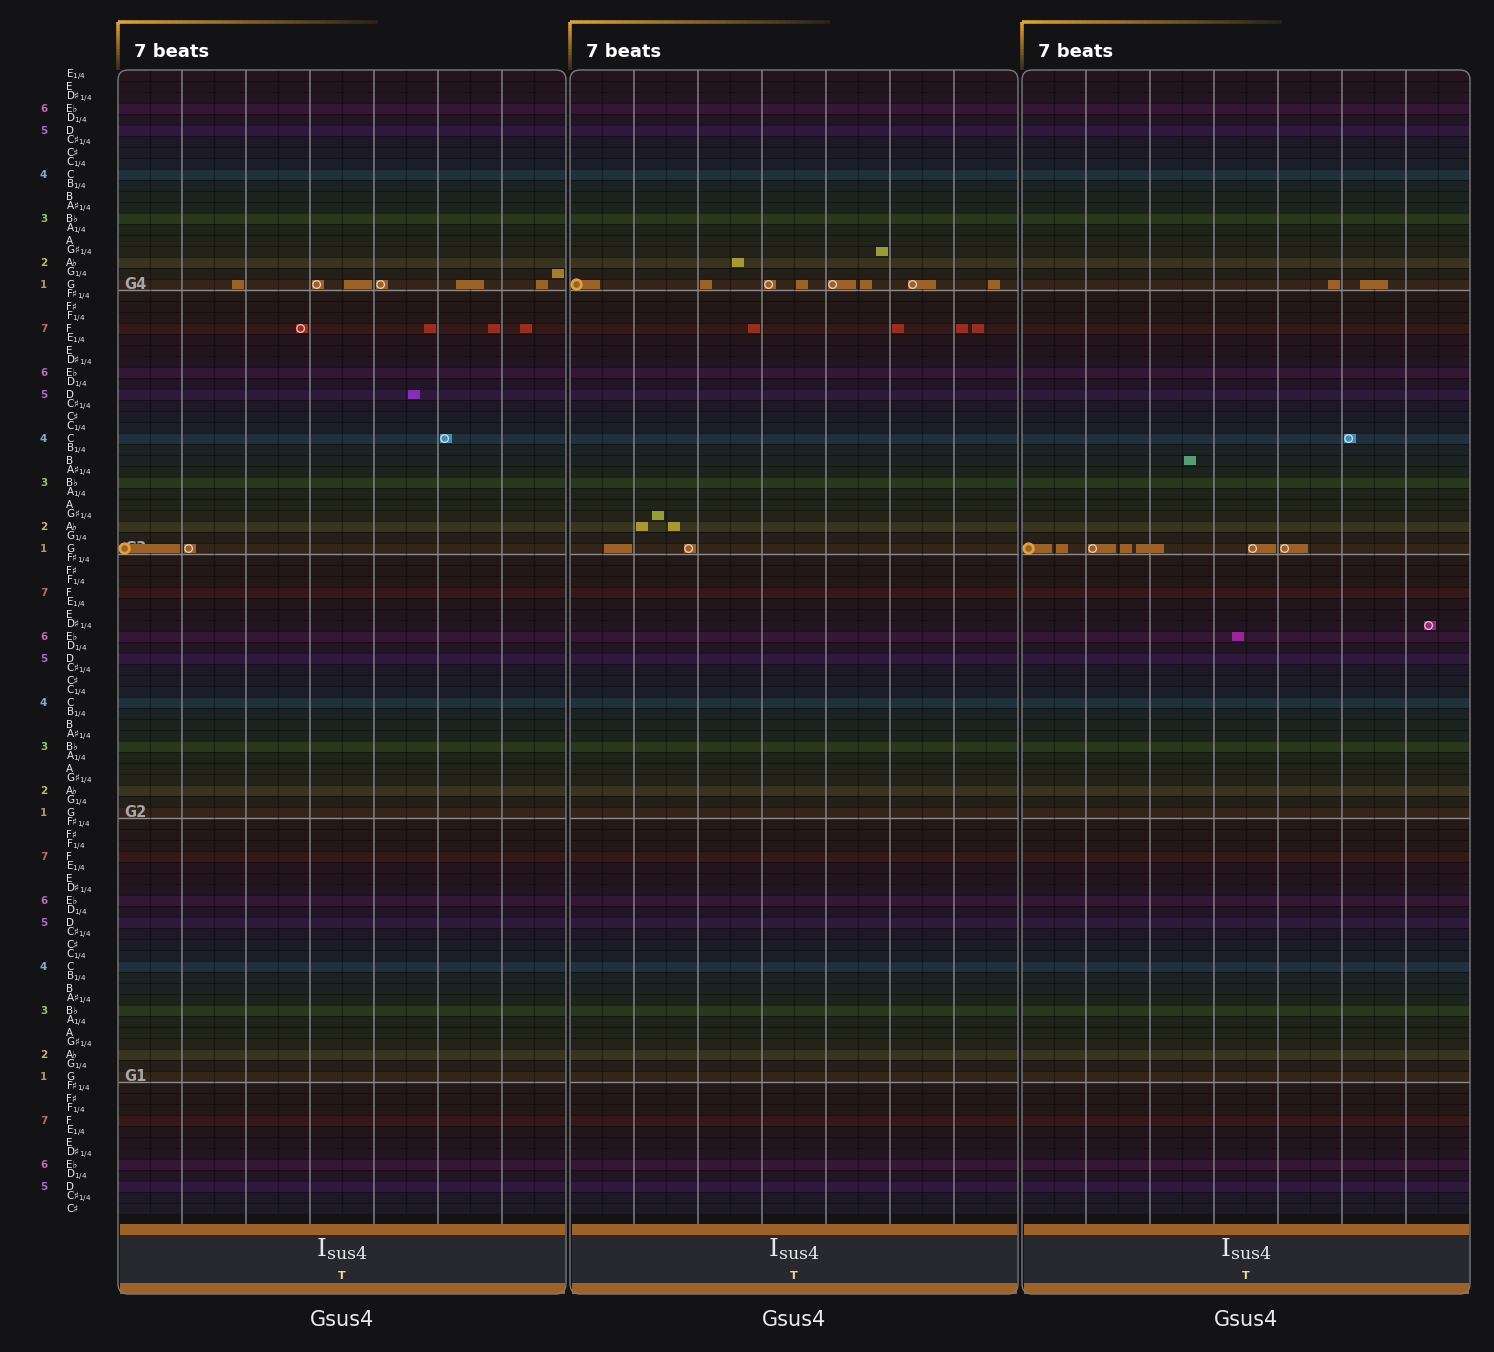
\includegraphics[width=0.75\textwidth]{yor_zarad_tabroll24.png}\\[0.5em]
  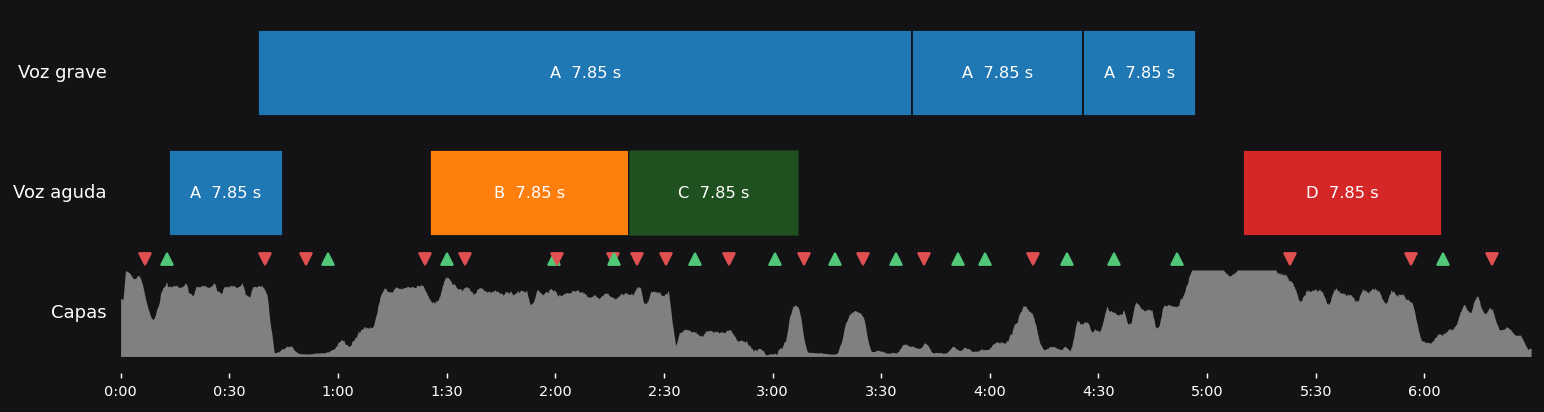
\includegraphics[width=\textwidth]{yor_zarad_mapa_ciclos.png}
  \caption{Yor Zarad: una página del tabroll24 (arriba) y el mapa de ciclos (abajo); misma lectura que la figura~\ref{fig:mata}.}\label{fig:yor}
\end{figure}

\paragraph{Armonía.} La fundamental está en I el 85\,\% del tiempo y en \fl2+ el 13\,\%: los 11 cambios entre compases
confiables son microtonales, todos entre I y \fl II+5 (el vaivén I5 $\leftrightarrow$ \fl II+5 aparece 6 veces). Es decir,
la armonía se mueve entre el eje de tónica y el eje neutro D--S, fuera del círculo de quintas. Desde 4:56 hasta el final el
centro está en Sol\sh+ (\fl2+). Fue la prueba ciega: su armonía acierta 87.8\,\%.

\paragraph{Melodía.} Los cuartos de tono ocupan el 16.8\,\%, con \fl2+ (8.4\,\%) y \fl6+ (3.5\,\%). La misma familia que Mata
Zyklek.

\paragraph{Metro.} El ciclo dura 28 corcheas ($R = 0.80$). Sin vecino en metro.

\clearpage
\subsection{Utzp}

La figura~\ref{fig:utzp-tarjeta} reúne la tarjeta y la tira de ciclos; la figura~\ref{fig:utzp}, una página del tabroll24 y el mapa de ciclos.

\begin{figure}[!h]
  \centering
  \begin{subfigure}[c]{0.42\textwidth}\centering
    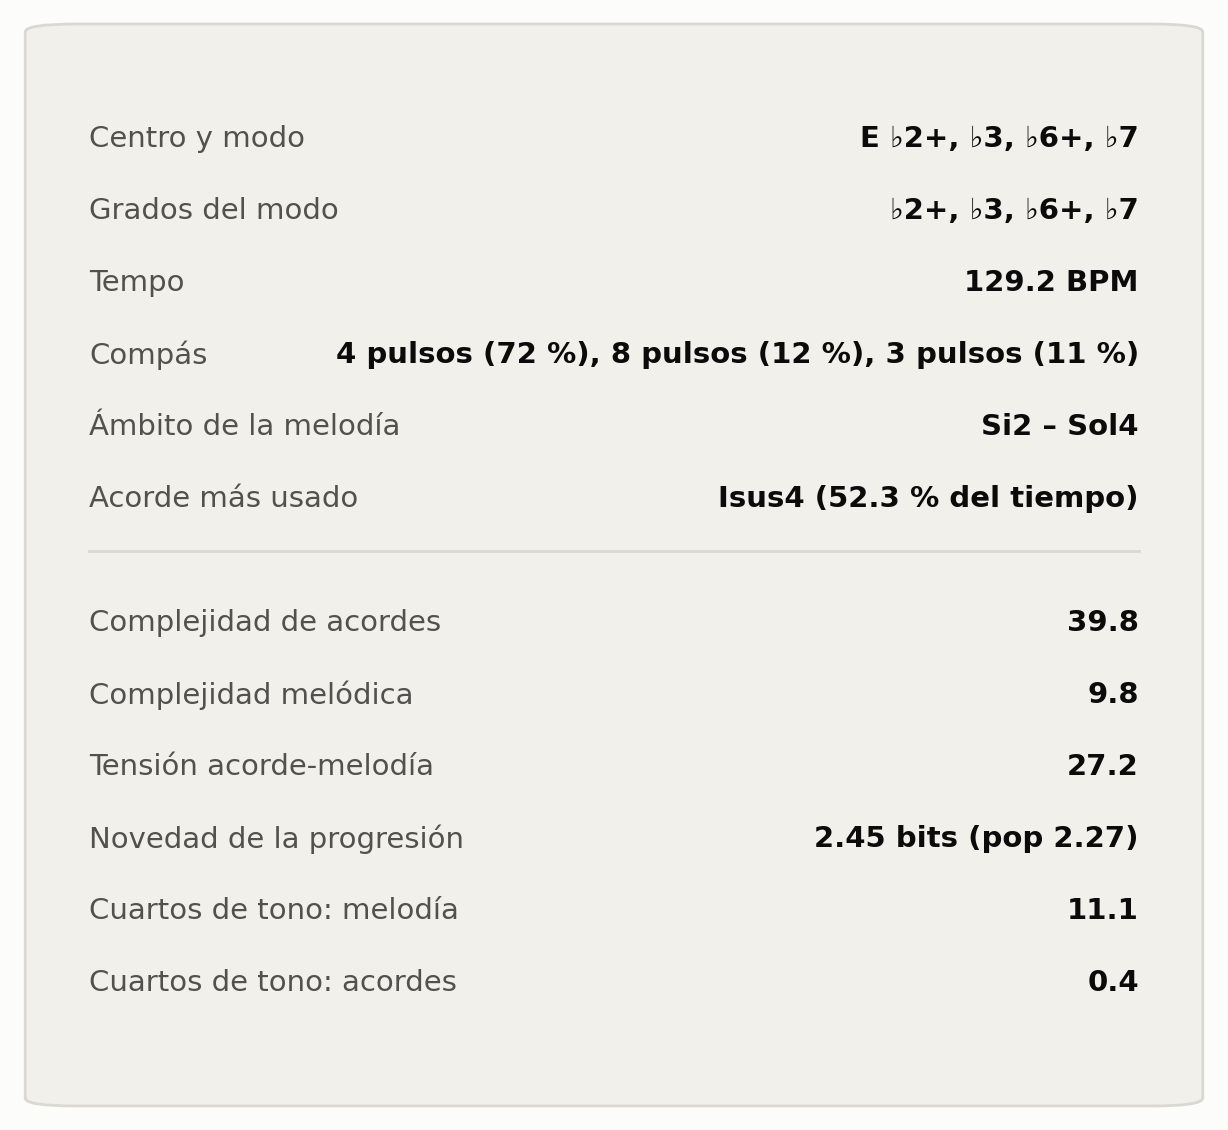
\includegraphics[width=\linewidth]{utzp_tarjeta.png}\caption{Tarjeta.}
  \end{subfigure}\hfill
  \begin{subfigure}[c]{0.55\textwidth}\centering
    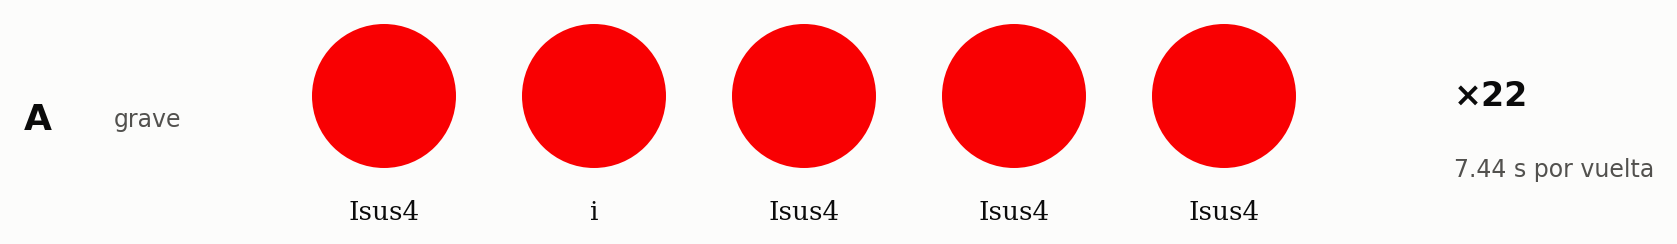
\includegraphics[width=\linewidth]{utzp_tira_de_ciclos.png}\caption{Ciclos repetidos.}
  \end{subfigure}
  \caption{Utzp: tarjeta y tira de ciclos; misma lectura que la figura~\ref{fig:fabienk-tarjeta}. Centro Mi, modo \fl2+, \fl3, \fl6+, \fl7; compases confiables: 82.2\,\%.}\label{fig:utzp-tarjeta}
\end{figure}

\begin{figure}[p]
  \centering
  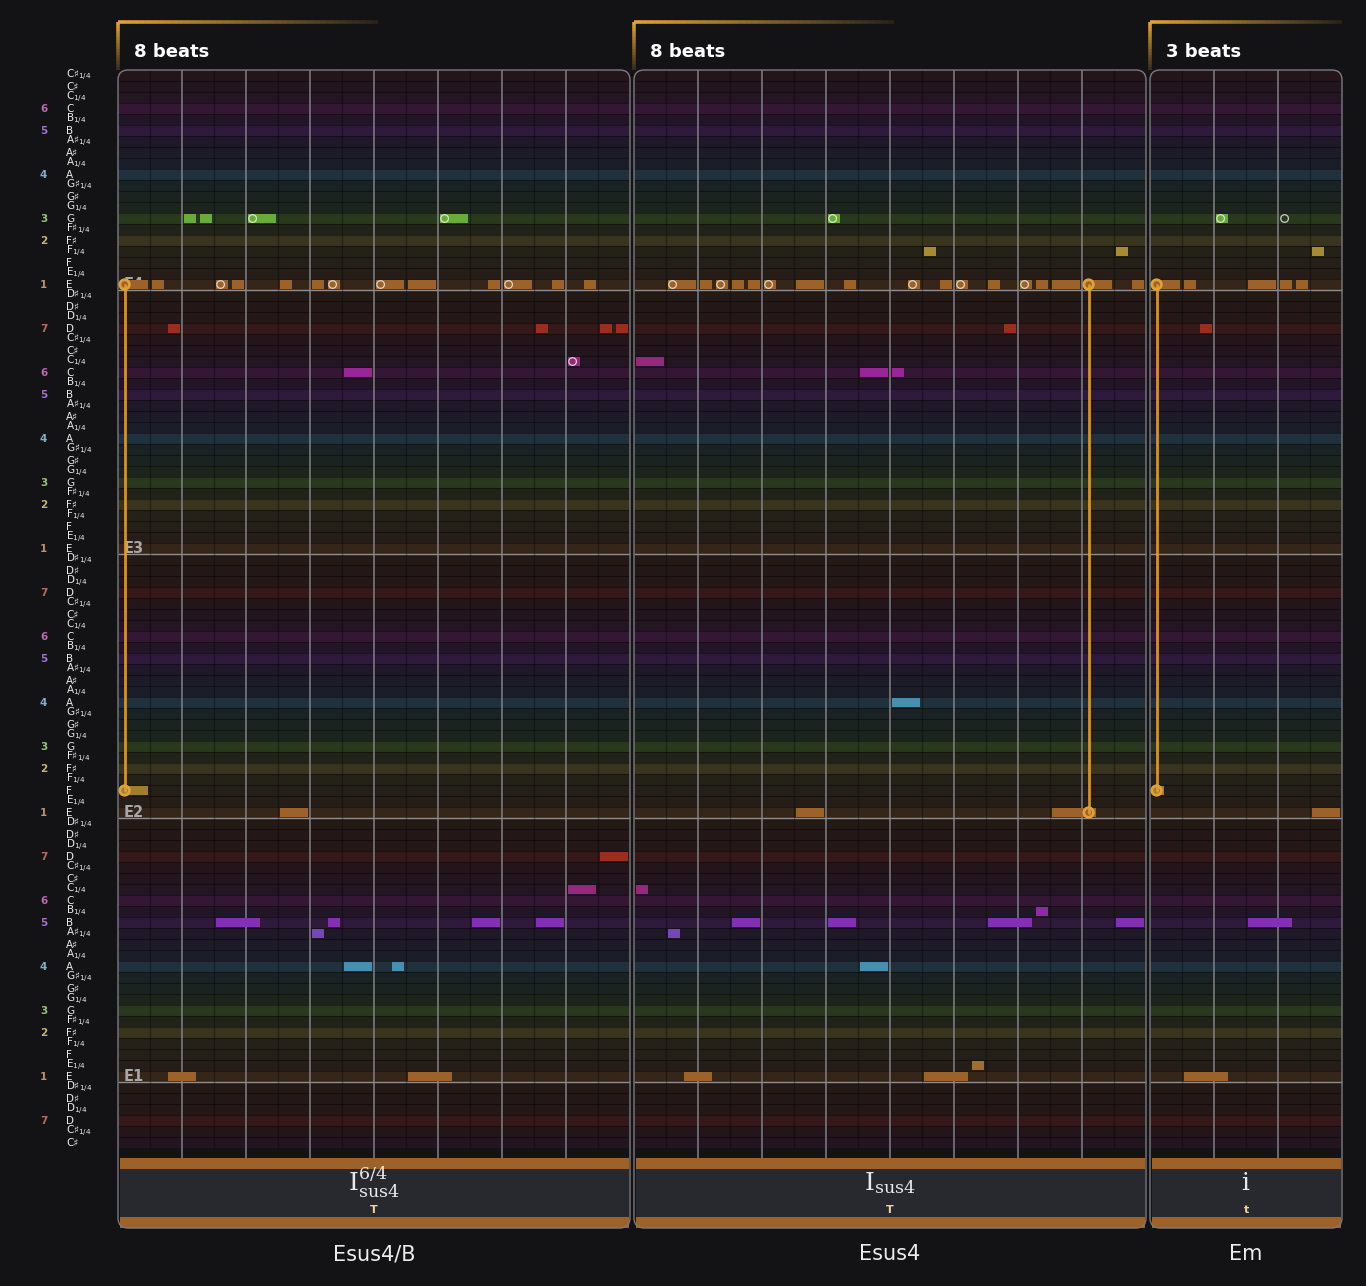
\includegraphics[width=0.75\textwidth]{utzp_tabroll24.png}\\[0.5em]
  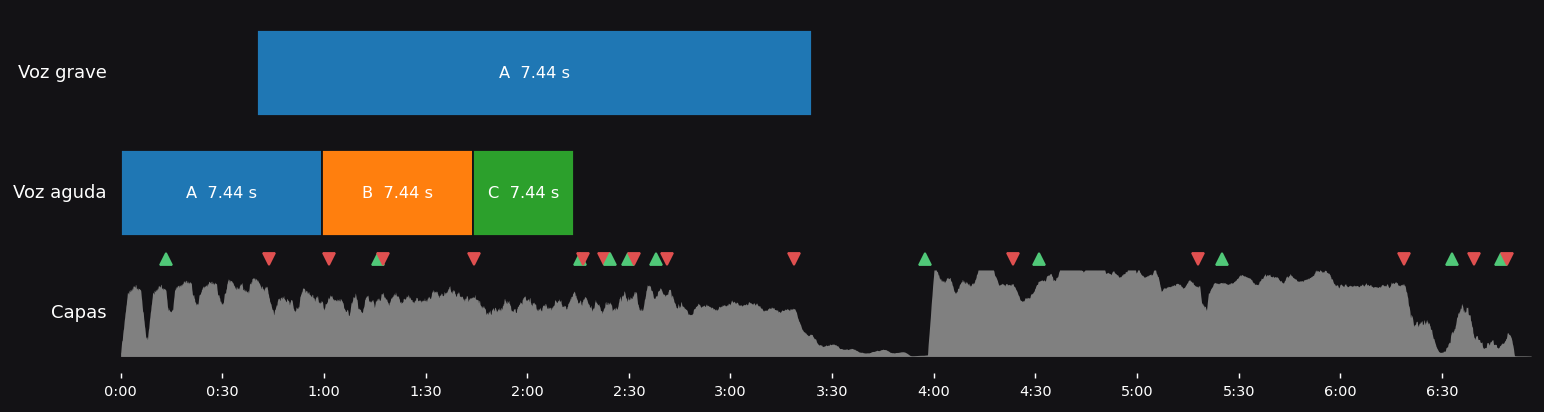
\includegraphics[width=\textwidth]{utzp_mapa_ciclos.png}
  \caption{Utzp: una página del tabroll24 (arriba) y el mapa de ciclos (abajo); misma lectura que la figura~\ref{fig:mata}.}\label{fig:utzp}
\end{figure}

\paragraph{Armonía.} Otro pedal: I el 96\,\% del tiempo (sus4 el 52\,\% y quinta sola el 31\,\%) y \fl VII el 4\,\%. De los
9 cambios, el 78\,\% son por segunda. La introducción está sobre Si (5) y entra a Mi por quinta abajo, como una cadencia de
dominante a tónica a gran escala.

\paragraph{Melodía.} La de mayor concentración: el 81.5\,\% de sus cuartos de tono cae en \fl6+ (6.0\,\%) y \fl2+ (3.0\,\%), y
\fl6+ aparece en todas las vueltas.

\paragraph{Metro y comparación.} Va en 4 (32 corcheas). Es la única canción con veredicto «síntesis de lenguajes
existentes»: en percentil por vecinos, su armonía es típica del rock (89), sus cuartos de tono del radif (32) y su metro del rock y del jazz (100),
pero ningún corpus explica la combinación.

\clearpage
\subsection{Angor}

La figura~\ref{fig:angor-tarjeta} reúne la tarjeta y la tira de ciclos; la figura~\ref{fig:angor}, una página del tabroll24 y el mapa de ciclos.

\begin{figure}[!h]
  \centering
  \begin{subfigure}[c]{0.42\textwidth}\centering
    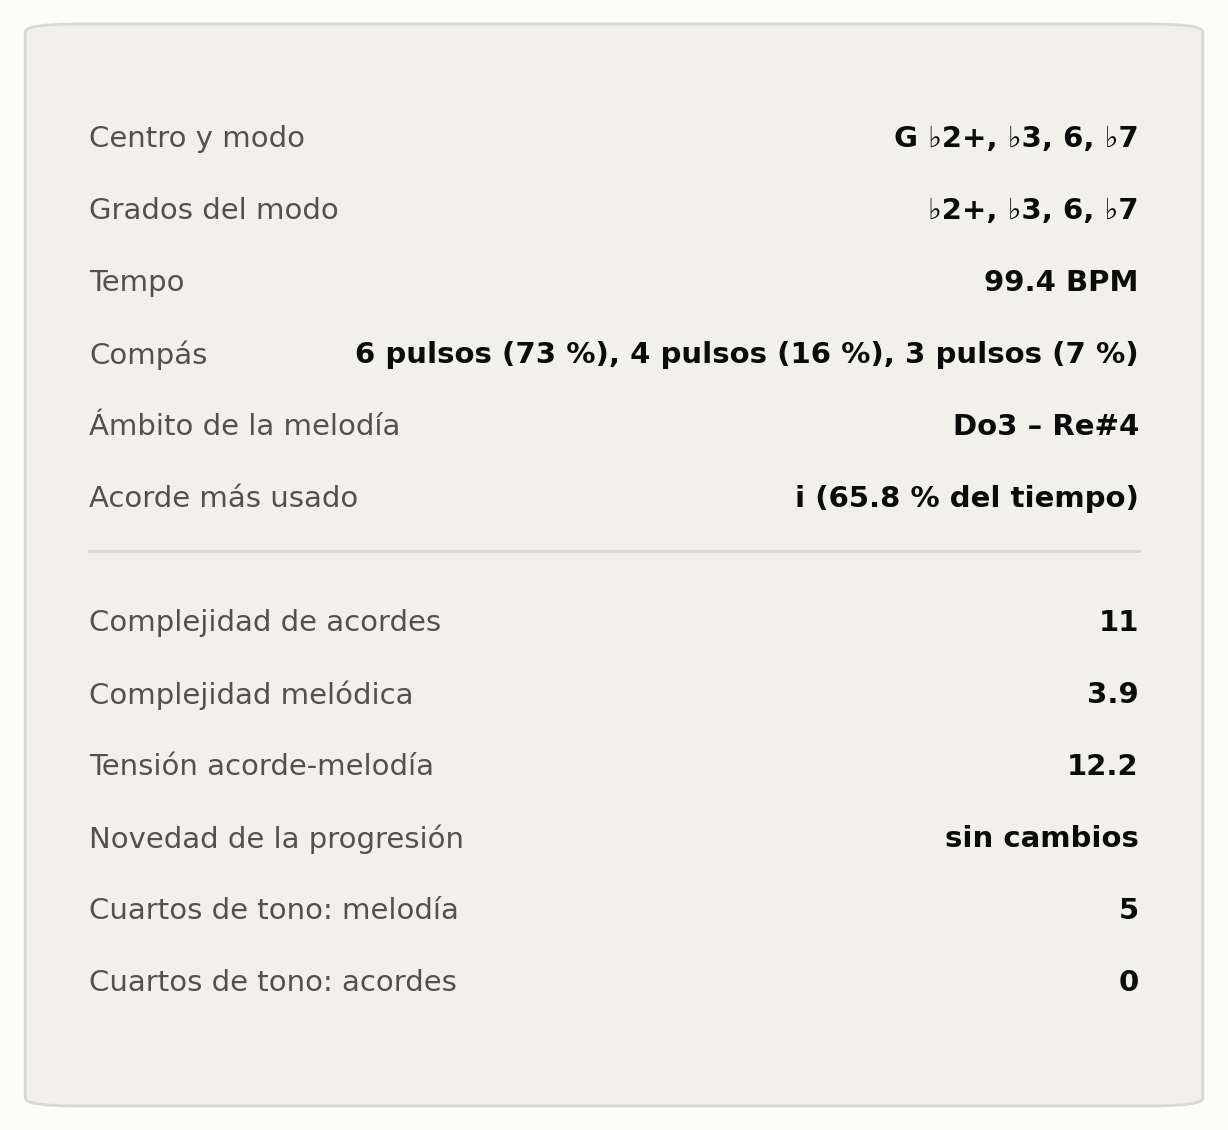
\includegraphics[width=\linewidth]{angor_tarjeta.png}\caption{Tarjeta.}
  \end{subfigure}\hfill
  \begin{subfigure}[c]{0.55\textwidth}\centering
    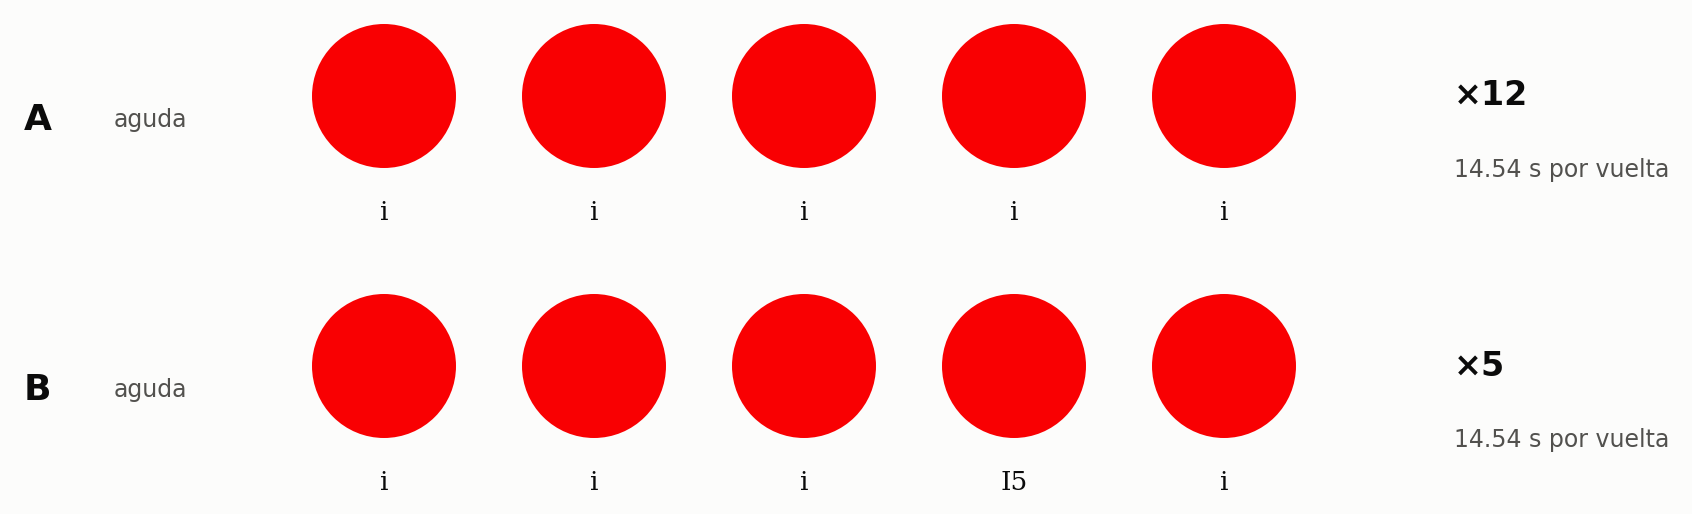
\includegraphics[width=\linewidth]{angor_tira_de_ciclos.png}\caption{Ciclos repetidos.}
  \end{subfigure}
  \caption{Angor: tarjeta y tira de ciclos; misma lectura que la figura~\ref{fig:fabienk-tarjeta}. Centro Sol, modo \fl2+, \fl3, 6, \fl7; compases confiables: 88.1\,\%.}\label{fig:angor-tarjeta}
\end{figure}

\begin{figure}[p]
  \centering
  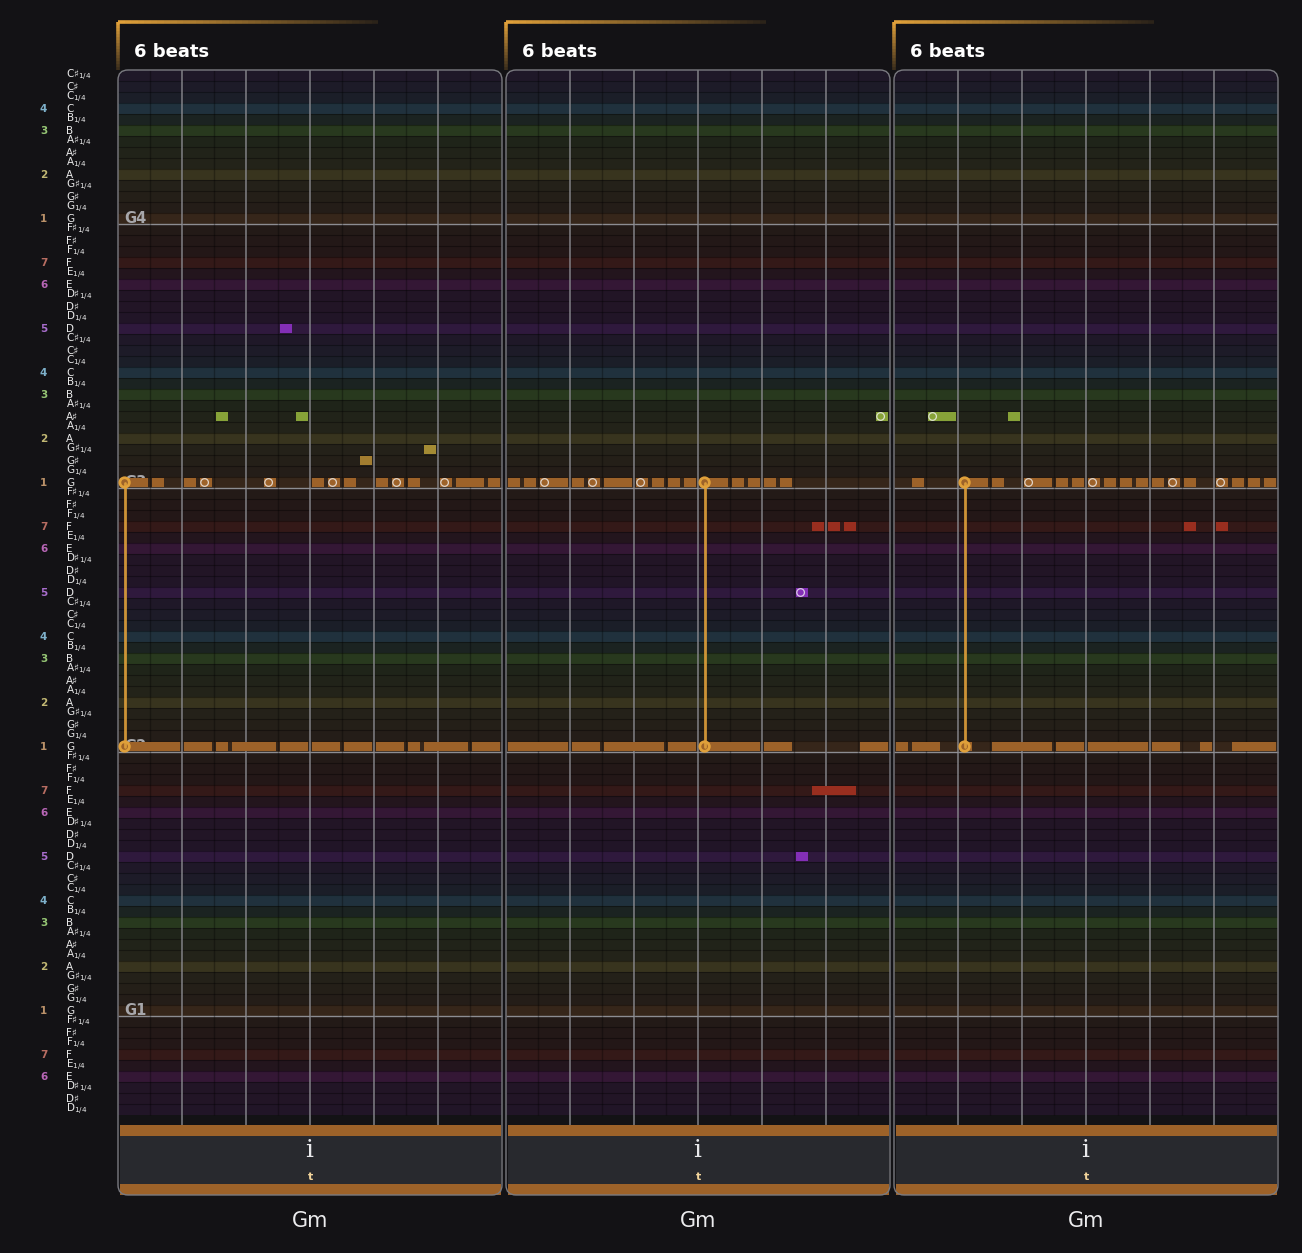
\includegraphics[width=0.75\textwidth]{angor_tabroll24.png}\\[0.5em]
  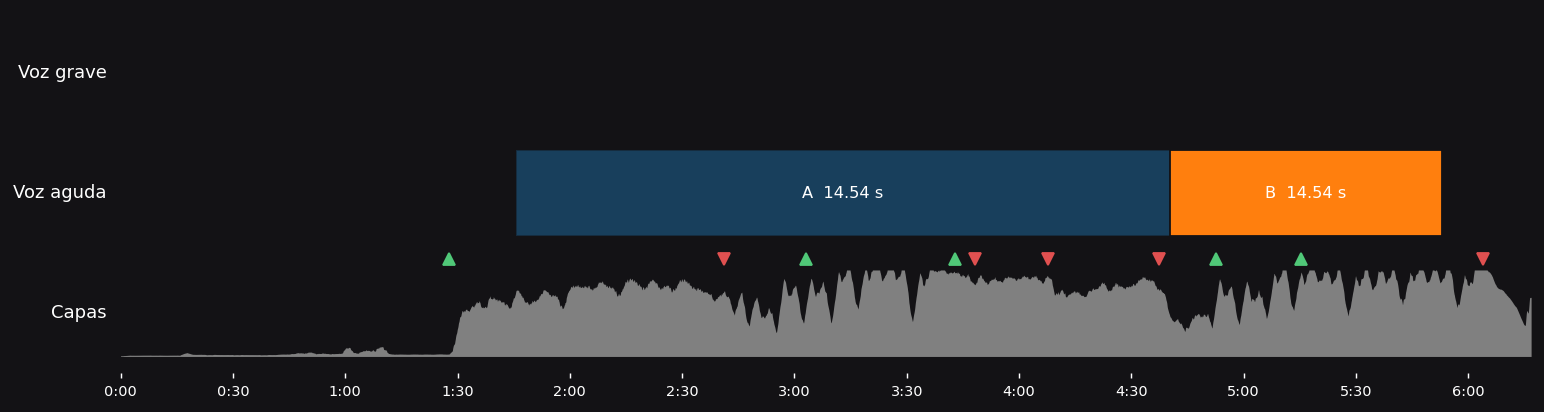
\includegraphics[width=\textwidth]{angor_mapa_ciclos.png}
  \caption{Angor: una página del tabroll24 (arriba) y el mapa de ciclos (abajo); misma lectura que la figura~\ref{fig:mata}.}\label{fig:angor}
\end{figure}

\paragraph{Armonía.} Un pedal casi absoluto: la fundamental está en I el 99.5\,\% del tiempo (i el 66\,\% y I5 el 31\,\%), sin
cambios entre compases confiables. En el test por bloques su armonía es idéntica a la de «Flying Microtonal Banana» de King
Gizzard, también un pedal sobre I.

\paragraph{Melodía.} Solo el 5\,\% de la melodía está en cuartos de tono, por debajo del piso de ruido, así que no cuenta
como evidencia. Aun así, \fl2+ aparece en el 92\,\% de las vueltas.

\paragraph{Metro.} La voz aguda repite un ciclo de 14.5~s y el mejor periodo es de 24 corcheas ($R = 0.83$); la voz grave no
tiene ciclos. Sin vecino en metro. Angor no tiene referencia de oído, así que sus cifras no se pueden evaluar.

\chapter{Discusión y limitaciones}\label{cap:discusion}

\section{Qué se puede afirmar}

La respuesta del trabajo descansa en la armonía y en la concentración de los cuartos de tono, que son las medidas más
fiables de la herramienta. La armonía acierta el 85\,\% en los compases confiables, incluso en la prueba ciega, y el
método no exagera la novedad: con rock real casi siempre encuentra vecino. La concentración de los cuartos de tono separa
a la banda del control con un margen amplio (48--82\,\% frente a 28--37\,\%), y ese margen es mayor que el error de la
herramienta.

\section{El parecido con el radif es de escala, no de influencia}

El test mide si la distribución de los cuartos de tono de una canción tiene vecinos cercanos entre las piezas del Radif
Corpus. Cuatro de las seis canciones los tienen: Mata Zyklek (percentil 13.5), Yor Zarad (10.9), Utzp (32.3) y Angor
(35.4). Las dos de la familia dórica, Sarniezz (3.9) y Fabienk (0.4), quedan por debajo del umbral de 5. Eso quiere decir
que la banda usa grados fijos en cuarto de tono y que, fuera del modo dórico, los reparte de forma parecida a esa tradición. No prueba que la banda conozca el radif ni que lo
haya tomado como modelo: el mismo reparto podría venir de otra tradición sin corpus simbólico disponible, como el maqam
árabe, o de una elección propia. Para hablar de influencia harían falta fuentes externas.

\section{El bloque de escala en 12 notas no discrimina}

En ese bloque los cuartos de tono se reparten entre los semitonos vecinos y la melodía se compara con corpus de 12 notas.
Las canciones de control de Primus, que no usan cuartos de tono, salen tan típicas como las de la banda («Tommy the Cat»
9.6 y «My Name Is Mud» 6.1 en el radif, frente a 8.7 a 9.6 de la banda). La causa más probable es que las melodías de los
corpus (la voz en el RS~200, una notación de tradición oral en el radif) no son del mismo tipo que la línea aguda que
extrae la herramienta, que en estas grabaciones es sobre todo guitarra y bajo. Los resultados de este bloque se informan,
pero no entran en la conclusión.

\section{El compás cambiante queda sin vecino, no demostrado como nuevo}

Mata Zyklek, Fabienk y Yor Zarad mezclan compases dentro de la misma canción. Ninguna pieza del RS~200 ni del iRealPro,
los dos corpus con compás de la comparación final, hace eso: cada pieza tiene un solo compás. SymbTr, con usules de 7, 9 y
10 tiempos pero también uno solo por pieza, se revisó y no entró en la comparación final. Por eso el resultado dice que no
hay antecedente en los corpus revisados, no que no lo haya en ninguna música. El estilo más cercano en la literatura es
el rock progresivo y el math rock, y el corpus que permitiría comprobarlo (ProgGP) no estuvo disponible.

\section{Comparación con los repertorios}\label{sec:repertorios}

Además de los corpus, el mismo cuaderno se corrió sobre canciones de los artistas que la banda o los analistas mencionan:
King Gizzard (9 temas de \emph{Flying Microtonal Banana}), Frank Zappa (6), King Crimson (6) y Gentle Giant (6), junto con
los tres controles de Primus. En total son 36 canciones medidas con los mismos parámetros. La
tabla~\ref{tab:repertorios} resume las tres medidas que distinguen a la banda y el veredicto del test por bloques.
Las métricas crudas de las 36 canciones, artista por artista, están en el apéndice (figuras~\ref{fig:tarjetas1}
y~\ref{fig:tarjetas2}).

\begin{table}[ht]
  \centering\small
  \caption{La banda frente a los repertorios comparados. \cuarto{} de tono: porcentaje medio de la melodía en cuartos de
  tono (rango entre paréntesis). Concentración: porcentaje de los cuartos de tono en los dos grados más usados. $R$: media
  del mejor periodo de repetición. «Existente»: canciones con veredicto «estilo existente».}\label{tab:repertorios}
  \begin{tabular}{@{}lrlllr@{}}
    \toprule
    Grupo & Temas & \cuarto{} de tono & Concentración & $R$ medio & Existente \\
    \midrule
    Angine de Poitrine & 6 & 16.1 (5.0--25.3) & 48--82 & 0.83 & 0 de 6 \\
    King Gizzard & 9 & 9.9 (3.4--28.0) & 59--100 & 0.69 & 4 de 9 \\
    King Crimson & 6 & 8.8 (0.1--25.0) & 37--82 & 0.52 & 1 de 6 \\
    Gentle Giant & 6 & 2.9 (0.9--6.4) & 38--87 & 0.51 & 0 de 6 \\
    Frank Zappa & 6 & 4.1 (1.6--7.0) & 31--54 & 0.45 & 3 de 6 \\
    Primus (control) & 3 & 11.3 (9.1--13.0) & 28--37 & 0.44 & 2 de 3 \\
    \bottomrule
  \end{tabular}
\end{table}

Tres observaciones matizan la conclusión.

\paragraph{La concentración solo se interpreta por encima del piso de ruido.} Gentle Giant y King Crimson tienen
concentraciones altas (hasta 87\,\% en «Playing the Game» y 82\,\% en «Discipline») con muy poco tiempo en cuartos de tono
(1.0 y 0.1\,\%). Ahí la concentración describe unos pocos errores de medición, no una escala. En Zappa y Gentle Giant el
tiempo en cuartos de tono queda incluso por debajo del de Primus. Lo que distingue a la banda es tener a la vez mucho tiempo
en cuartos de tono, por encima del piso de ruido, y concentrado en pocos grados; por eso el test por bloques solo cuenta la concentración cuando hay al menos 10~s de
melodía en cuarto de tono. El perfil de la figura~\ref{fig:perfil}
lo muestra frente a Primus y King Gizzard: en cuartos de tono en la melodía, la banda tiene la mediana más alta y King
Gizzard la dispersión más amplia, mientras que Primus, sin cuartos de tono reales, se queda en el piso de ruido.

\begin{figure}[htbp]
  \centering
  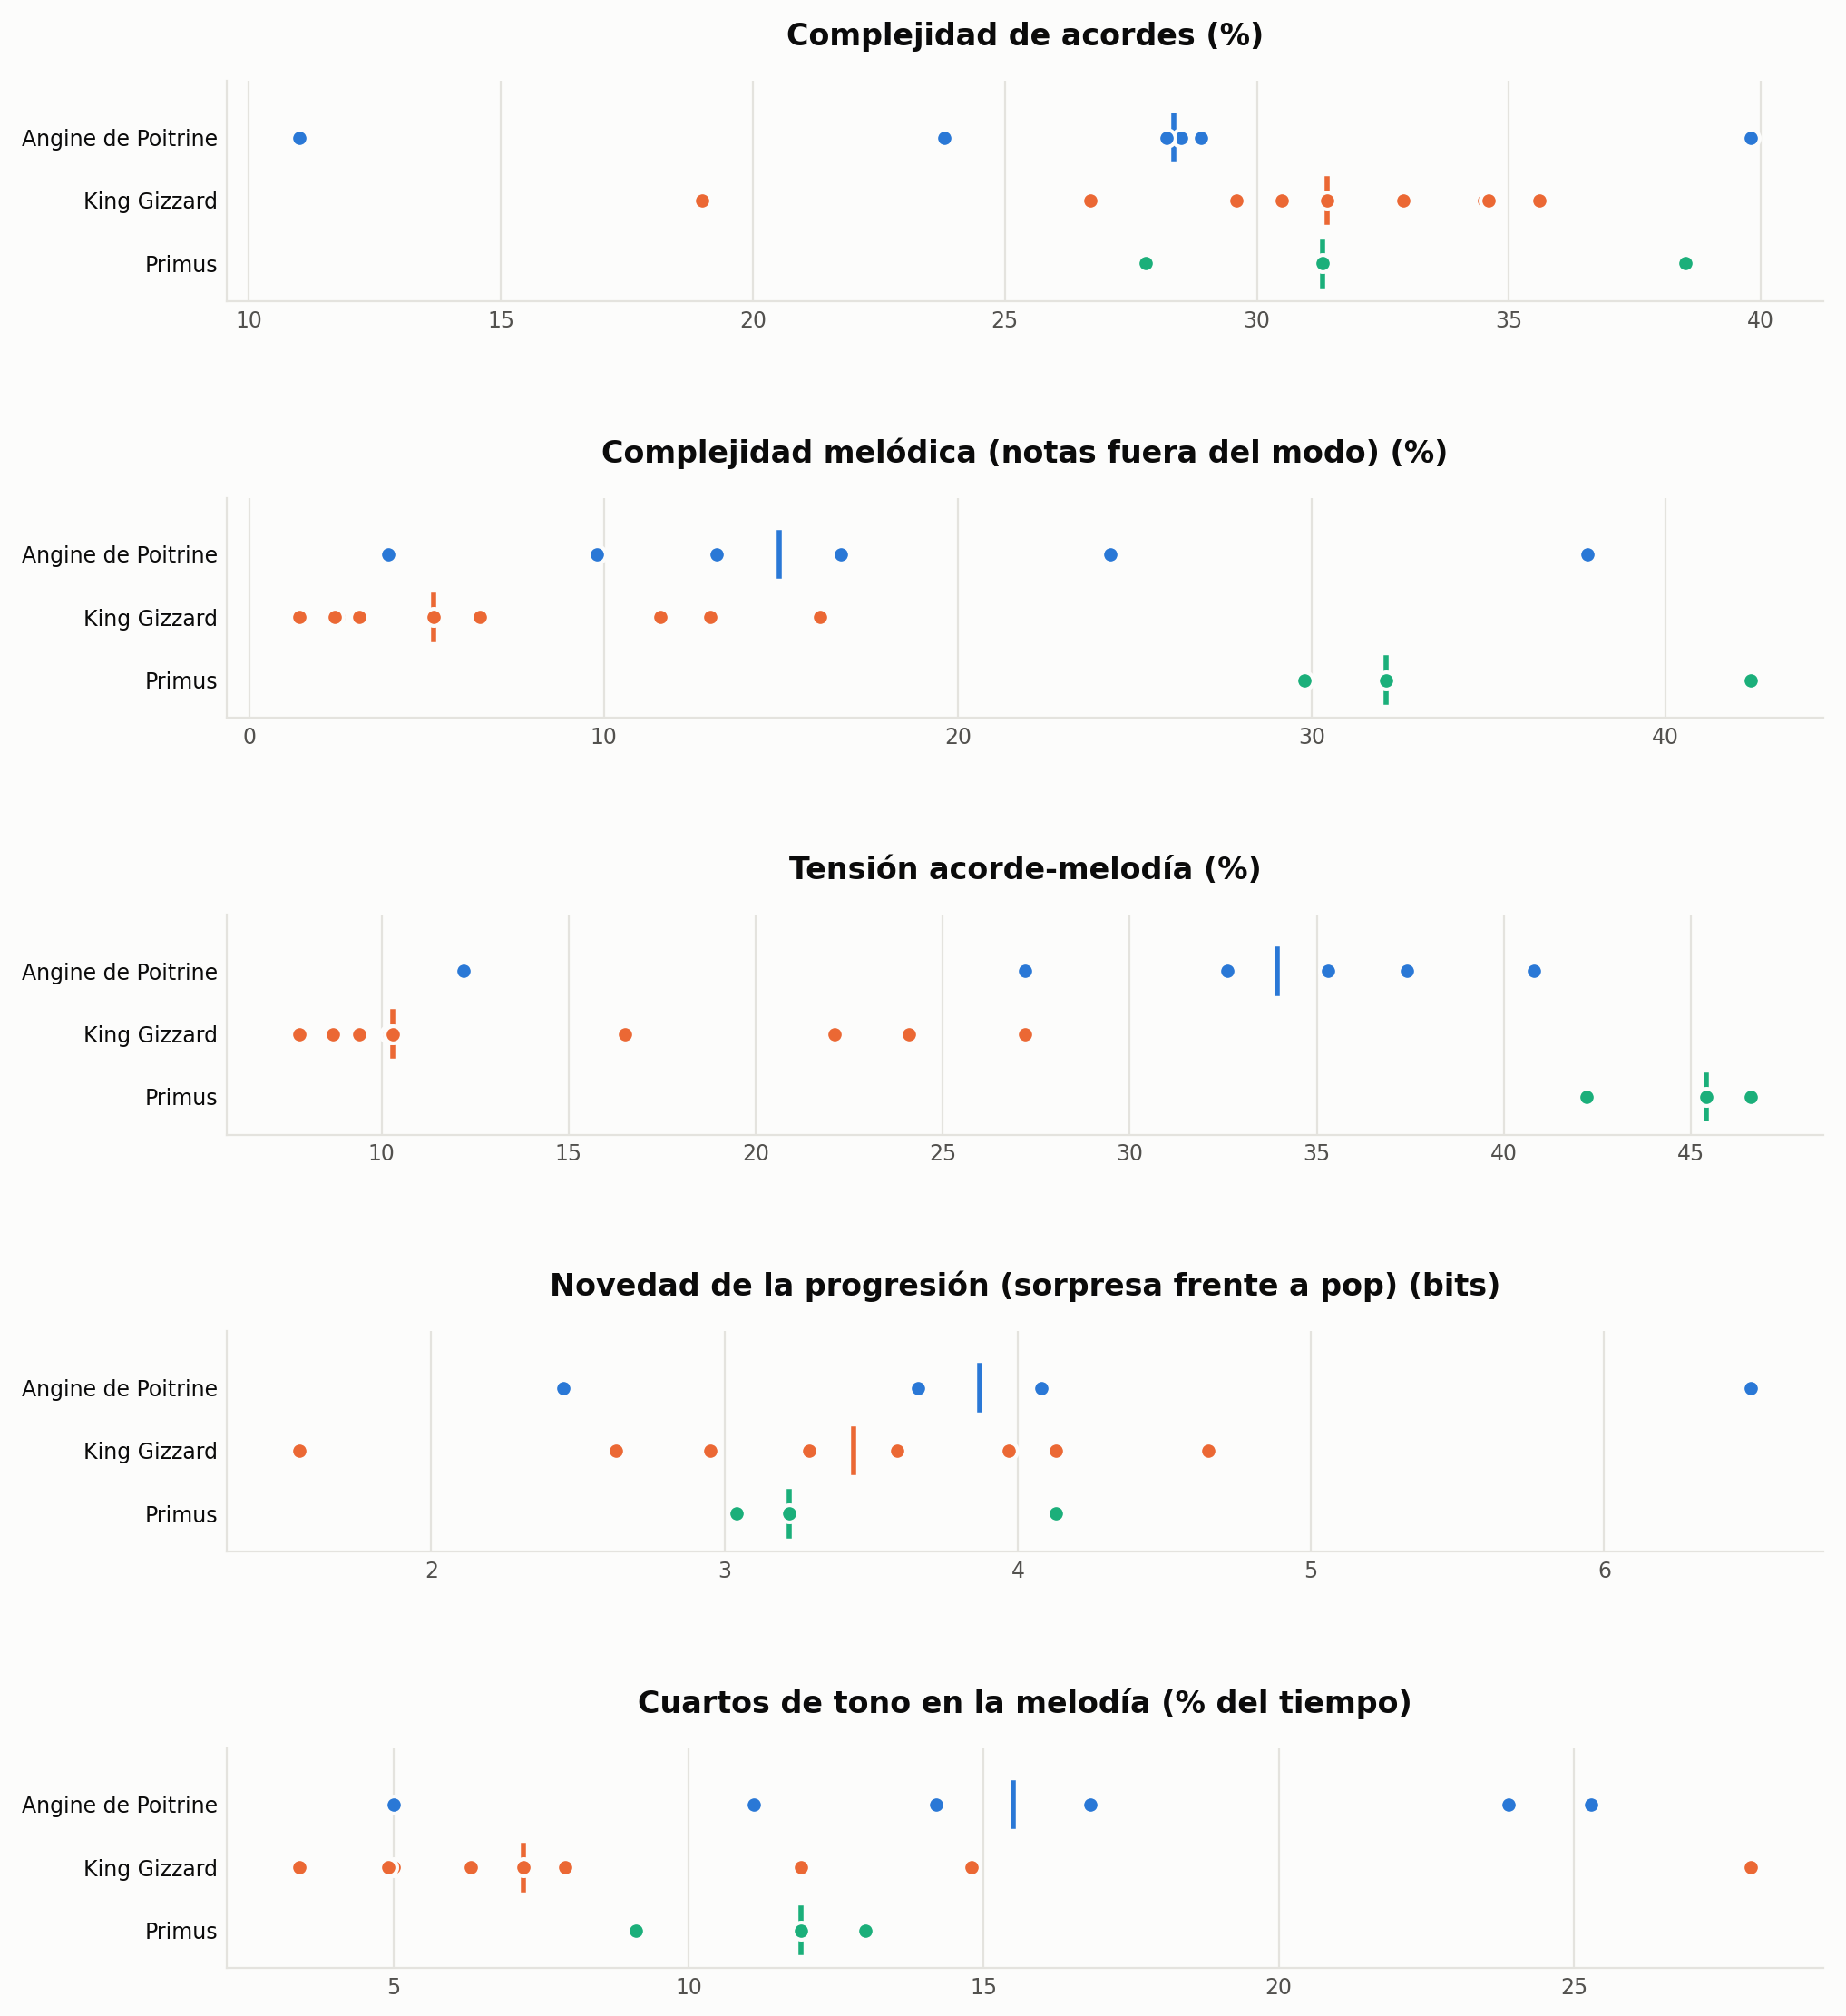
\includegraphics[width=0.85\textwidth]{g_perfil.png}
  \caption{Perfil estructural: la banda (azul) frente a Primus (verde, control) y King Gizzard (naranja). Cada punto es una canción; la raya vertical, la mediana del grupo.}\label{fig:perfil}
\end{figure}

\paragraph{King Gizzard es el vecino más cercano, y comparte dos de los tres rasgos.} Es el único repertorio con cuartos
de tono reales y concentrados (por ejemplo «Doom City», con 28\,\% y 95\,\%) y con ciclos casi tan estables ($R$ medio de
0.69, frente a 0.83 de la banda y 0.44--0.52 del rock progresivo). Su familia de cuartos de tono es la frigia
(\fl2+ y \fl6+ son sus dos grados principales en 5 de sus 9 temas;
«Doom City» combina \fl2+ con 7+). Lo que King Gizzard no tiene es la familia dórica de Sarniezz y Fabienk, y casi la
mitad de sus temas (4 de 9) sí reciben el veredicto «estilo existente (rock)». La figura~\ref{fig:comparar-kg} mide la
distancia de cada canción de la banda a cada tema de King Gizzard y de Zappa, primero solo en los grados en cuarto de tono
y luego en conjunto, con los tres temas de Primus como referencia.

\begin{figure}[htbp]
  \centering
  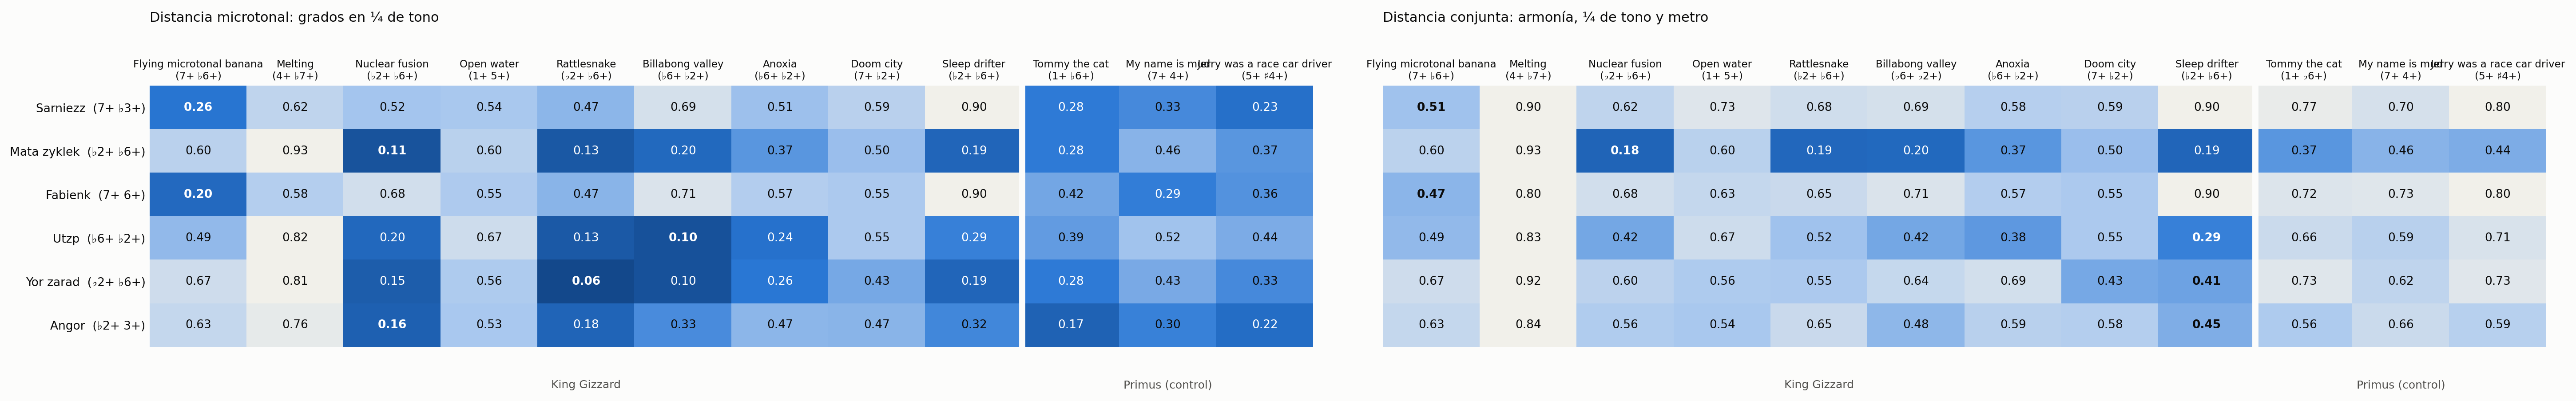
\includegraphics[width=\textwidth]{g_comparar_kg.png}\\[1em]
  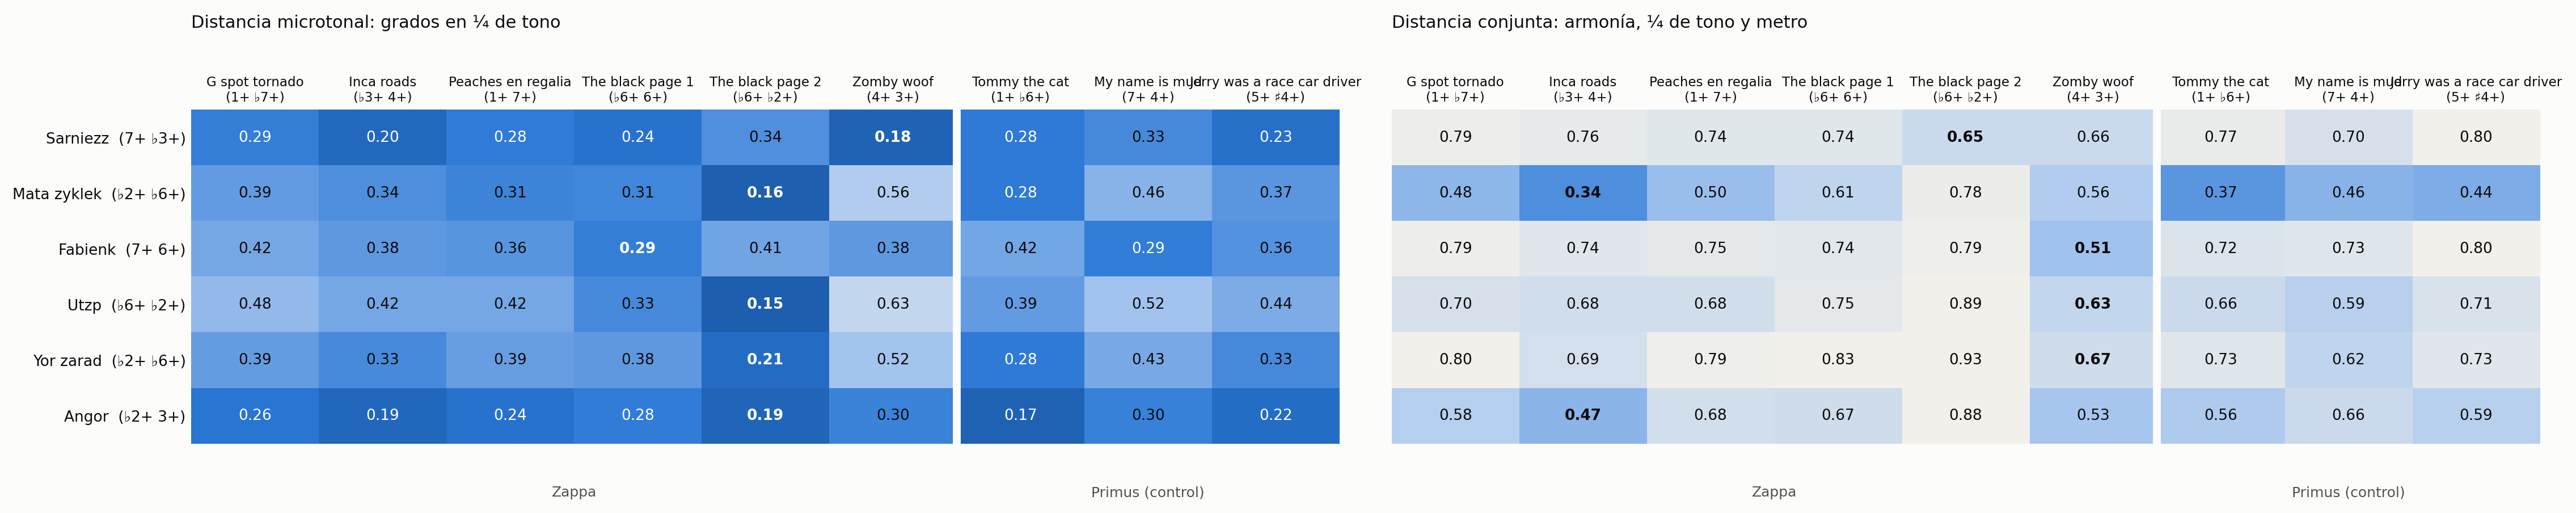
\includegraphics[width=\textwidth]{g_comparar_zappa.png}
  \caption{Distancia de Jensen-Shannon de cada canción de la banda (filas, con sus dos grados en cuarto de tono más usados) a King Gizzard (arriba) y Zappa (abajo), con Primus como control. Izquierda: solo cuartos de tono; derecha: armonía, cuartos de tono y metro. 0 = iguales; más oscuro = más cerca. Bajo cada tema, sus dos grados en cuarto de tono más usados; en negrita, el tema más cercano a cada canción.}\label{fig:comparar-kg}
\end{figure}

\paragraph{El rock progresivo tampoco es un «estilo existente» para estos corpus.} Ninguna canción de Gentle Giant recibe el
veredicto «estilo existente»: todas quedan sin vecino en metro o en armonía, por la misma razón que la banda, que es que
los corpus con compás no tienen piezas con compás cambiante. Por eso el veredicto «sin vecino en metro» no basta, por sí
solo, para afirmar que la banda es nueva: dice que el rock progresivo y el math rock no están representados en los corpus
disponibles. La conclusión del trabajo se apoya, en cambio, en la armonía (fuera de todos los corpus, con la calibración
que lo respalda) y en la melodía (cuartos de tono fijos por encima del piso de ruido, con una familia que ningún corpus ni
repertorio tiene).

Los ciclos de los repertorios refuerzan esta lectura. Las canciones de Zappa, King Crimson y Gentle Giant tienen periodos
variados (de 6 a 32 corcheas, con picos en 5 y en 7 en «The Black Page», «Fracture», «Frame by Frame» y «Level Five»), pero
mucho menos estables que los de la banda: el compás irregular es común en el rock progresivo; la repetición casi idéntica
del looper, no. La figura~\ref{fig:comparar-gg} da las mismas distancias frente a King Crimson y Gentle Giant.

\begin{figure}[htbp]
  \centering
  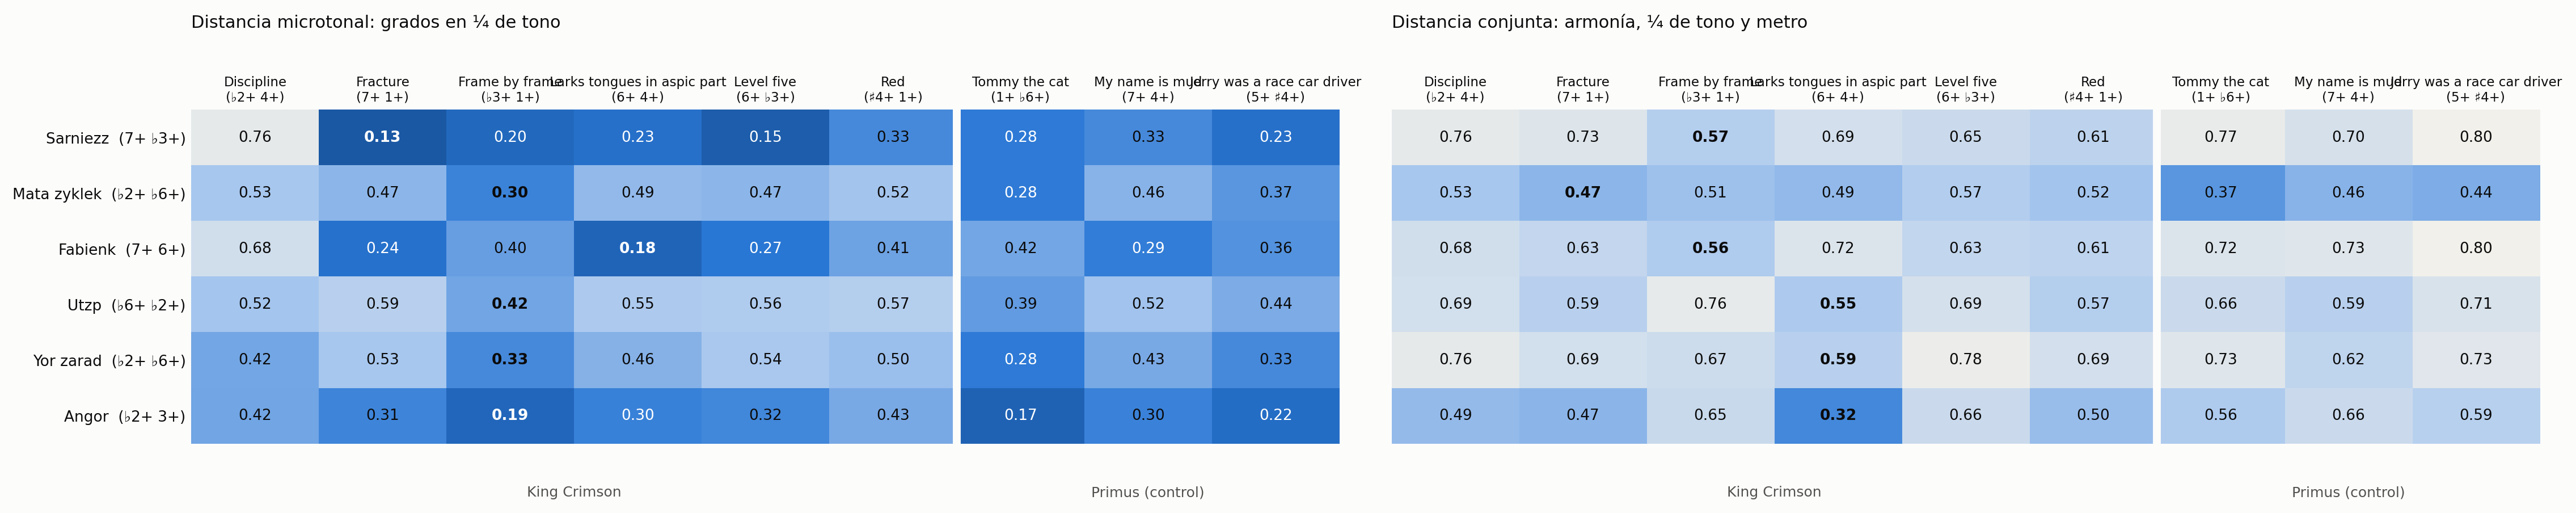
\includegraphics[width=\textwidth]{g_comparar_kc.png}\\[1em]
  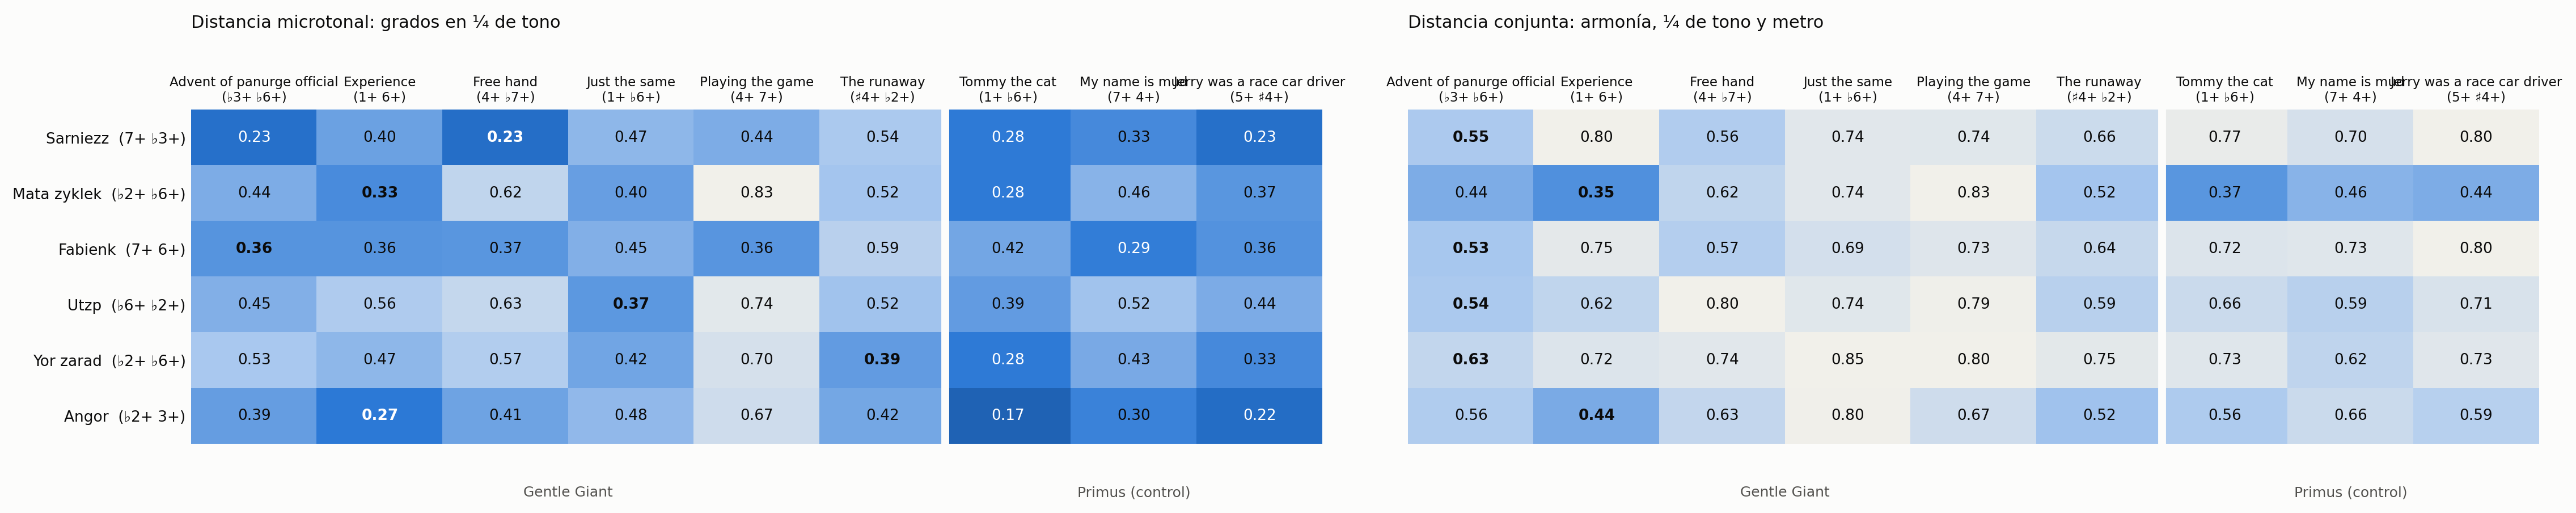
\includegraphics[width=\textwidth]{g_comparar_gg.png}
  \caption{Las mismas distancias frente a King Crimson (arriba) y Gentle Giant (abajo); misma lectura que la figura~\ref{fig:comparar-kg}.}\label{fig:comparar-gg}
\end{figure}

\section{¿Es 24-EDO la rejilla adecuada?}

Todo el análisis supone que la banda toca en 24-EDO, porque así están construidos sus instrumentos. Conviene comprobar que
otra rejilla no describiría mejor lo que suena. La tabla~\ref{tab:edos} lleva los grados que usa el disco a otros
sistemas de afinación y mide cuánto se desafinan.
La figura~\ref{fig:edos} lo muestra grado por grado.

\begin{figure}[htbp]
  \centering
  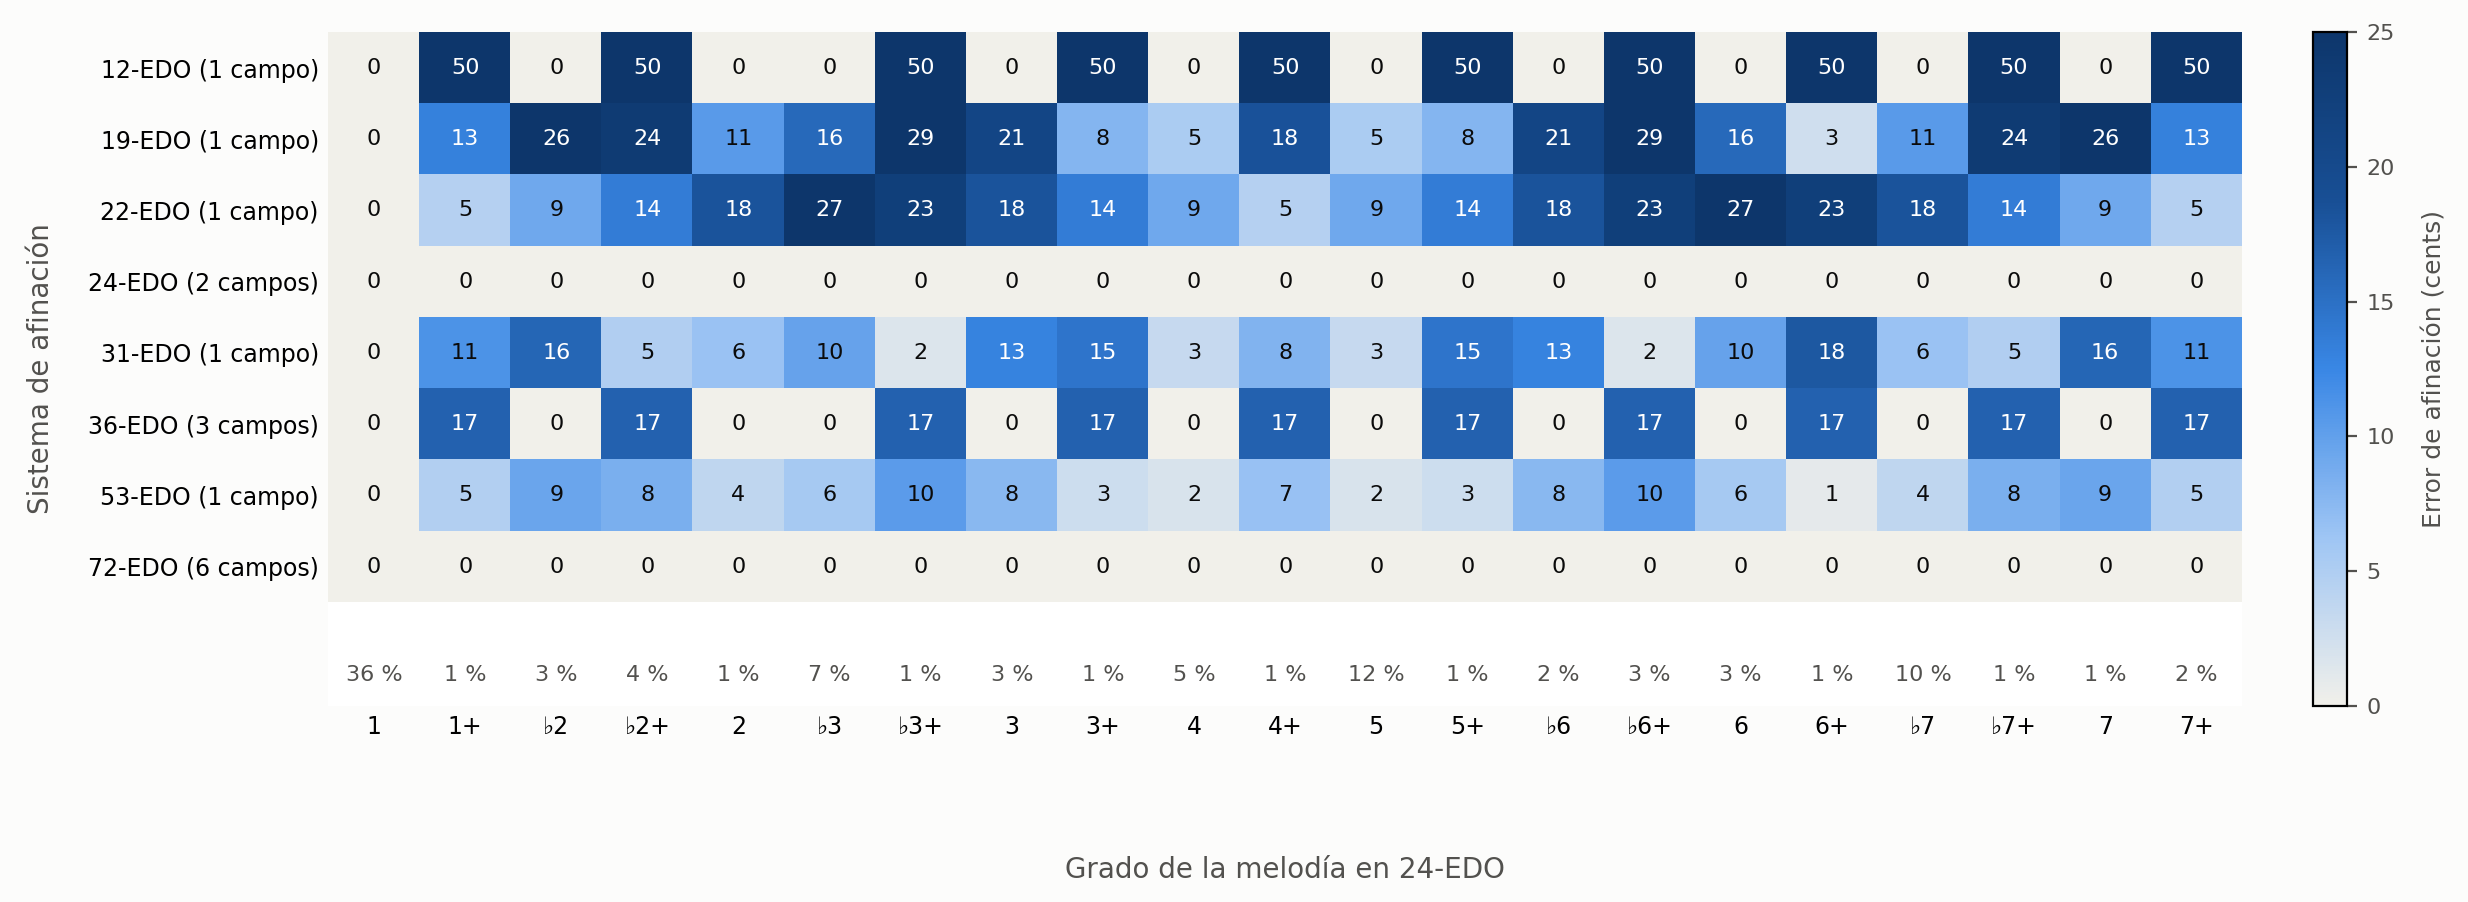
\includegraphics[width=\textwidth]{g_equivalencias_edo.png}
  \caption{Error al llevar cada grado de la melodía de 24-EDO a otro sistema (cents; blanco = sin error, azul oscuro = 25 o más). Entre paréntesis, los campos de quintas de cada sistema; abajo, el uso de cada grado en el álbum.}\label{fig:edos}
\end{figure}

\begin{table}[ht]
  \centering\small
  \caption{Los grados del disco en otros sistemas: error medio (en cents) de los grados usados y de los grados en cuarto
  de tono, y número de campos de quintas.}\label{tab:edos}
  \begin{tabular}{@{}lrrrrl@{}}
    \toprule
    Sistema & Paso & Campos & Error de los grados & Error de los \cuarto & Grados \cuarto{} que se funden \\
    \midrule
    12-EDO & 100.0 & 1 & 8.0 & 50.0 & todos \\
    19-EDO & 63.2 & 1 & 8.9 & 19.2 & \fl2+, \fl3+, \fl6+, \fl7+ \\
    22-EDO & 54.5 & 1 & 9.9 & 14.9 & \fl3+, \fl6+ \\
    \textbf{24-EDO} & \textbf{50.0} & \textbf{2} & \textbf{0.0} & \textbf{0.0} & \textbf{ninguno} \\
    31-EDO & 38.7 & 1 & 4.8 & 7.6 & ninguno \\
    36-EDO & 33.3 & 3 & 2.7 & 16.7 & ninguno \\
    53-EDO & 22.6 & 1 & 3.2 & 6.9 & ninguno \\
    72-EDO & 16.7 & 6 & 0.0 & 0.0 & ninguno \\
    \bottomrule
  \end{tabular}
\end{table}

Por construcción, 24-EDO y sus múltiplos (72-EDO) representan sin error lo que mide la herramienta; el resultado
interesante está en los demás. En 19 y 22-EDO varios grados en cuarto de tono se funden con un grado regular: en ambos
desaparece \fl6+, y con él la familia frigia (\fl2+, \fl6+). En 31 y 53-EDO los grados sobreviven, con errores medios de 3 a 8 cents, pero esos sistemas
tienen un solo campo de quintas: la separación entre la armonía, en el campo regular, y los grados de la melodía, en el
otro campo, deja de existir, y con ella el «desplazamiento de campos» de la sección~\ref{sec:res-haba}. 24-EDO es, entonces,
el sistema más pequeño que conserva a la vez los grados que usa la banda y la estructura de dos campos que organiza su
música.

La escala de la melodía del disco, tomando la variante más usada de cada grado móvil, es 1 · \fl2+ · \fl3 · 4 · 5 · 6 ·
\fl7: un dórico con la segunda neutra. Las fundamentales quedan en el campo regular y la melodía usa sus grados en cuarto de
tono en el otro campo.

\section{Modos compartidos con King Gizzard}

El modo de cada canción, descrito por los grados 2, 3, 6 y 7, permite una comparación más fina que el reparto de grados.
Utzp (\fl2+, \fl3, \fl6+, \fl7) tiene exactamente el mismo modo que «Nuclear Fusion», «Sleep Drifter» y «Billabong
Valley» de King Gizzard; «Rattlesnake» y «Doom City» comparten la segunda neutra \fl2+ sobre un frigio. Ninguna canción de
King Gizzard tiene el modo de Mata Zyklek y Yor Zarad (\fl2+, 3, \fl6+, \fl7), con tercera mayor, ni el dórico con
cuartos de tono en la melodía de Fabienk y Sarniezz. El parentesco con King Gizzard es, por tanto, real pero parcial: comparten
la familia frigia, no las otras dos.

\section{Límites de la herramienta}

\begin{itemize}
  \item \textbf{Melodía.} La melodía acierta entre el 37 y el 66\,\% según la canción. El cuello de botella es separar las
  capas del looper: en muchos cuadros la melodía no aparece entre los picos de la saliencia, y ni la estructura del
  looper, ni el estéreo, ni un separador mejor la destapan.
  \item \textbf{Armonía de Sarniezz.} Acierta el 58\,\%, por su riff cromático de cuartos de tono, su acorde sus2 y su bajo
  un cuarto de tono bajo.
  \item \textbf{Centro tonal fuera de la banda.} La elección del centro falla en algunas canciones ajenas: «Tommy the Cat»
  sale en Sol en vez de Mi.
  \item \textbf{Pocas canciones.} El álbum tiene seis canciones y solo cuatro tienen referencia.
  \item \textbf{Corpus.} Ningún corpus de armonía tiene cuartos de tono, y los corpus microtonales simbólicos no
  representan necesariamente la afinación real de una interpretación. Los corpus de rock y pop tienen sesgos de selección
  y de transcripción.
  \item \textbf{Separación.} La comparación entre separadores se hizo en una sola canción; no basta para generalizar.
\end{itemize}

\section{Primus y las influencias}

La comparación con Primus muestra parecidos puntuales: «Tommy the Cat» comparte con Fabienk y Sarniezz el centro (Mi, el de la
partitura, aunque la herramienta lo elija mal), el modo dórico y las fundamentales 1, \fl3 y \fl7, y «My Name Is Mud» es un pedal, como Mata Zyklek. Pero Primus no tiene ciclos
de looper ni cuartos de tono concentrados, y cambia más de acorde. Como ninguna fuente pública lo cita como influencia, se
presenta solo como comparación propia. Del mismo modo, King Gizzard es el vecino más cercano en conjunto, pero la banda no
lo cita; lo propone un analista.

\chapter{Conclusiones y trabajo futuro}\label{cap:conclusiones}

\section{Conclusiones}

El trabajo se propuso estudiar tres dimensiones, y hay una conclusión por cada una.

\paragraph{Armonía: no encaja en ningún estilo.} La banda toma elementos de varios estilos, pero no encaja en ninguno. El
37.5\,\% de los casos queda sin vecino, frente al 5.2\,\% de las piezas reales de rock, y ninguna canción pasa de 17.7
cuando una pieza típica daría 50. Las fundamentales son de rock modal, sin dominante, pero desplazadas hacia \fl VII y
\fl III, a una zona que ningún corpus ocupa.

\paragraph{Melodía: lo nuevo.} Dos grados en cuarto de tono concentran entre el 48 y el 82\,\% de los cuartos de tono de
cada canción. Son notas fijas de la escala, no adornos, y forman dos familias. La frigia (\fl2+, \fl6+) es la más común en
el radif persa y en King Gizzard. La dórica (7+, 6+, \fl3+) no aparece en ningún corpus medido.

\paragraph{Síntesis: un híbrido.} Hay ciclos de 5 y de 7 tiempos, como dice la banda; la armonía se parece a la del rock
modal; los cuartos de tono se reparten como en el radif; y el vecino más cercano es King Gizzard.

\medskip
La respuesta a la pregunta del trabajo es que la música de Angine de Poitrine no corresponde a un estilo existente. Es una
combinación nueva de lenguajes que ya existían, con un elemento propio: los cuartos de tono como notas fijas de la escala.

Además del resultado, el trabajo deja una herramienta abierta que transcribe y analiza en 24-EDO desde el audio, y un
método de comparación con corpus que aplica a los corpus el error de la propia herramienta y está calibrado para no
exagerar la novedad.

\section{Trabajo futuro}

El siguiente paso es un tabroll que mejore solo, para cualquier canción, mediante un ciclo de cuatro pasos:
\begin{enumerate}
  \item sintetizar partituras de Guitar Pro con cuartos de tono;
  \item entrenar con ellas un transcriptor en 24-EDO;
  \item transcribir canciones nuevas;
  \item validar con referencias de oído.
\end{enumerate}
Así habría datos sin límite, sin transcribir a mano. Además:
\begin{itemize}
  \item \textbf{Melodía:} tratar las vueltas del looper como varias tomas de la misma frase, para separar las capas.
  \item \textbf{Armonía:} elegir el centro tonal de forma robusta en cualquier canción.
  \item \textbf{Datos:} un corpus de maqam árabe y el acceso a ProgGP, para comprobar el compás cambiante frente al rock
  progresivo.
  \item \textbf{Producto:} un tabroll web interactivo, el análisis de otros músicos microtonales, como King Gizzard y
  Sevish, y su uso en la enseñanza.
\end{itemize}


% Referencias. Las marcadas \pv requieren comprobación antes de la entrega (contrastar cada DOI en Crossref).
\begin{thebibliography}{99}
\addcontentsline{toc}{chapter}{Referencias}

\bibitem[Bennett(2026)]{bennett2026}
Bennett, D. (2026). \emph{How Angine de Poitrine use Microtonality} [video]. David Bennett Music Theory, YouTube,
21 de marzo de 2026. \url{https://www.youtube.com/watch?v=91QWp6Ygx7c}

\bibitem[Bittner et~al.(2022)]{bittner2022}
Bittner, R. M., Bosch, J. J., Rubinstein, D., Meseguer-Brocal, G., y Ewert, S. (2022). A lightweight
instrument-agnostic model for polyphonic note transcription and multipitch estimation. \emph{Proc.\ IEEE ICASSP},
781--785. \url{https://doi.org/10.1109/ICASSP43922.2022.9746549}

\bibitem[Bozkurt(2008)]{bozkurt2008}
Bozkurt, B. (2008). An automatic pitch analysis method for Turkish maqam music. \emph{Journal of New Music Research},
37(1), 1--13.

\bibitem[Bozkurt et~al.(2009)]{bozkurt2009}
Bozkurt, B., Yarman, O., Karaosmanoğlu, M. K., y Akkoç, C. (2009). Weighing diverse theoretical models on Turkish maqam
music against pitch measurements. \emph{Journal of New Music Research}, 38(1), 45--70.
\url{https://doi.org/10.1080/09298210903147673}

\bibitem[Bozkurt et~al.(2014)]{bozkurt2014}
Bozkurt, B., Ayangil, R., y Holzapfel, A. (2014). Computational analysis of Turkish makam music: Review of
state-of-the-art and challenges. \emph{Journal of New Music Research}, 43(1), 3--23.

\bibitem[Broze y Shanahan(2013)]{broze2013}
Broze, Y., y Shanahan, D. (2013). Diachronic changes in jazz harmony: A cognitive perspective. \emph{Music Perception},
31(1), 32--45. \url{https://doi.org/10.1525/mp.2013.31.1.32}

\bibitem[Chorościan(2018)]{choroscian2018}
Chorościan, E. (2018). Alois Hába's microtonal systems and their practical use in selected string quartets.
\emph{Kwartalnik Młodych Muzykologów UJ}, 38(3), 47--78. \url{https://doi.org/10.4467/23537094KMMUJ.18.033.9734}

\bibitem[Davis y Mermelstein(1980)]{davis1980}
Davis, S. B., y Mermelstein, P. (1980). Comparison of parametric representations for monosyllabic word recognition in
continuously spoken sentences. \emph{IEEE Transactions on Acoustics, Speech, and Signal Processing}, 28(4), 357--366.
\url{https://doi.org/10.1109/TASSP.1980.1163420}

\bibitem[de Cheveigné y Kawahara(2002)]{decheveigne2002}
de Cheveigné, A., y Kawahara, H. (2002). YIN, a fundamental frequency estimator for speech and music. \emph{Journal of
the Acoustical Society of America}, 111(4), 1917--1930. \url{https://doi.org/10.1121/1.1458024}

\bibitem[de Clercq y Temperley(2011)]{declercq2011}
de Clercq, T., y Temperley, D. (2011). A corpus analysis of rock harmony. \emph{Popular Music}, 30(1), 47--70.
\url{https://doi.org/10.1017/S026114301000067X}

\bibitem[Dunlevie(2026)]{dunlevie2026}
Dunlevie, J. (2026). Angine de Poitrine, the French Canadian costumed microtonal duo breaking the internet. \emph{ABC
News}, 20 de mayo de 2026.
\url{https://www.abc.net.au/news/2026-05-20/angine-de-poitrine-microtonal-math-rock-quebec/106593634}

\bibitem[Ellis(2007)]{ellis2007}
Ellis, D. P. W. (2007). Beat tracking by dynamic programming. \emph{Journal of New Music Research}, 36(1), 51--60.
\url{https://doi.org/10.1080/09298210701653344}

\bibitem[Endres y Schindelin(2003)]{endres2003}
Endres, D. M., y Schindelin, J. E. (2003). A new metric for probability distributions. \emph{IEEE Transactions on
Information Theory}, 49(7), 1858--1860. \url{https://doi.org/10.1109/TIT.2003.813506}

\bibitem[Farhat(1990)]{farhat1990}
Farhat, H. (1990). \emph{The Dastgah Concept in Persian Music}. Cambridge University Press.
\url{https://doi.org/10.1017/CBO9780511470233}

\bibitem[Gedik y Bozkurt(2010)]{gedik2010}
Gedik, A. C., y Bozkurt, B. (2010). Pitch-frequency histogram-based music information retrieval for Turkish music.
\emph{Signal Processing}, 90(4), 1049--1063. \url{https://doi.org/10.1016/j.sigpro.2009.06.017}

\bibitem[Hába(1927)]{haba1927}
Hába, A. (1927). \emph{Neue Harmonielehre des diatonischen, chromatischen Viertel-, Drittel-, Sechstel- und
Zwölftel-Tonsystems}. Traducción del checo por el autor, revisión de E. Steinhard. Fr.\ Kistner \& C.\ F.\ W. Siegel.

\bibitem[Holzapfel et~al.(2014)]{holzapfel2014}
Holzapfel, A., Krebs, F., y Srinivasamurthy, A. (2014). Tracking the «odd»: Meter inference in a culturally diverse
music corpus. \emph{Proc.\ ISMIR}, 425--430.

\bibitem[Hooktheory(s.\,f.)]{hooktheory}
Hooktheory (s.\,f.). \emph{TheoryTab}: análisis armónicos de los álbumes \emph{30} (Adele, 2021), \emph{Everything to
Everyone} (Reneé Rapp, 2022), \emph{Gettin' Old} (Luke Combs, 2023), \emph{Happier Than Ever} (Billie Eilish, 2021),
\emph{Midnights} (Taylor Swift, 2022), \emph{Montero} (Lil Nas X, 2021), \emph{Solar Power} (Lorde, 2021),
\emph{$-$ (Subtract)} (Ed Sheeran, 2023) y \emph{Think Later} (Tate McRae, 2023). \url{https://www.hooktheory.com/theorytab}
\pv[: enlace exacto de cada análisis de álbum]

\bibitem[Huron(2006)]{huron2006}
Huron, D. (2006). \emph{Sweet Anticipation: Music and the Psychology of Expectation}. MIT Press.

\bibitem[Jin(2015)]{jin2015}
Jin, Y. (2015). \emph{A Study of Quarter-Tone Music for Solo Violin by Alois Hába} [tesis de doctorado en artes
musicales]. College-Conservatory of Music, University of Cincinnati.

\bibitem[Kanani et~al.(2025)]{kanani2025}
Kanani, M., O'Leary, S., y McDermott, J. (2025). Radif Corpus: A symbolic dataset for non-metric Iranian classical
music. \emph{Proc.\ ISMIR}. arXiv:2507.10456.

\bibitem[KEXP(2026)]{kexp2026}
KEXP (2026). \emph{Angine de Poitrine: KEXP session feature} [artículo], 25 de marzo de 2026.
\url{https://www.kexp.org/read/2026/3/25/angine-de-poitrine-kexp-session-feature/}

\bibitem[Karaosmanoğlu(2012)]{karaosmanoglu2012}
Karaosmanoğlu, M. K. (2012). A Turkish makam music symbolic database for music information retrieval: SymbTr.
\emph{Proc.\ ISMIR}, 223--228.

\bibitem[Kim et~al.(2018)]{kim2018}
Kim, J. W., Salamon, J., Li, P., y Bello, J. P. (2018). CREPE: A convolutional representation for pitch estimation.
\emph{Proc.\ IEEE ICASSP}. \url{https://doi.org/10.1109/ICASSP.2018.8461329}

\bibitem[King Gizzard and the Lizard Wizard(2017)]{kinggizzard2017}
King Gizzard and the Lizard Wizard (2017). \emph{Flying Microtonal Banana} [álbum y nota de lanzamiento], 24 de febrero
de 2017. \url{https://kinggizzardandthelizardwizard.com/release/flying-microtonal-banana}

\bibitem[Krumhansl(1990)]{krumhansl1990}
Krumhansl, C. L. (1990). \emph{Cognitive Foundations of Musical Pitch}. Oxford University Press.

\bibitem[Lendvai(1971)]{lendvai1971}
Lendvai, E. (1971). \emph{Béla Bartók: An Analysis of His Music}. Kahn \& Averill.


\bibitem[Lerdahl y Jackendoff(1983)]{lerdahl1983}
Lerdahl, F., y Jackendoff, R. (1983). \emph{A Generative Theory of Tonal Music}. MIT Press.

\bibitem[Lin(1991)]{lin1991}
Lin, J. (1991). Divergence measures based on the Shannon entropy. \emph{IEEE Transactions on Information Theory},
37(1), 145--151. \url{https://doi.org/10.1109/18.61115}

\bibitem[Little(2019)]{little2019}
Little, T. (2019). \emph{The Quarter-Tone Problem (and Hába's «Field Shifting» Solution)} [video]. Classical Nerd,
YouTube, 17 de enero de 2019. \url{https://www.youtube.com/watch?v=E_Z0q7jqyqI}

\bibitem[Loth et~al.(2023)]{loth2023}
Loth, J., Sarmento, P., Carr, C. J., Zukowski, Z., y Barthet, M. (2023). ProgGP: From GuitarPro tablature neural
generation to progressive metal production. \emph{Proc.\ CMMR}. arXiv:2307.05328.

\bibitem[Lu et~al.(2024)]{lu2024}
Lu, W.-T., Wang, J.-C., Kong, Q., y Hung, Y.-N. (2024). Music source separation with band-split RoPE transformer.
\emph{Proc.\ IEEE ICASSP}, 481--485. \url{https://doi.org/10.1109/ICASSP48485.2024.10446843}

\bibitem[Mathémusique(2026)]{mathemusique2026}
Mathémusique [Lascabettes, P.] (2026). \emph{Comprendre ANGINE DE POITRINE} [video]. YouTube, 16 de mayo de 2026.
\url{https://www.youtube.com/watch?v=96D7DKZh-es}

\bibitem[Mauch y Dixon(2014)]{mauch2014}
Mauch, M., y Dixon, S. (2014). pYIN: A fundamental frequency estimator using probabilistic threshold distributions.
\emph{Proc.\ IEEE ICASSP}, 659--663. \url{https://doi.org/10.1109/ICASSP.2014.6853678}

\bibitem[McClain(2026)]{mcclain2026}
McClain, L. (2026). \emph{Angine de Poitrine Explained} [video]. YouTube, 7 de septiembre de 2026.
\url{https://www.youtube.com/watch?v=kWv5zjsjoHw}

\bibitem[McFee et~al.(2015)]{mcfee2015}
McFee, B., Raffel, C., Liang, D., Ellis, D. P. W., McVicar, M., Battenberg, E., y Nieto, O. (2015). librosa: Audio and
music signal analysis in Python. \emph{Proc.\ SciPy}, 18--24. \url{https://doi.org/10.25080/Majora-7b98e3ed-003}

\bibitem[MIDI Manufacturers Association(1996)]{midi1996}
MIDI Manufacturers Association (1996). \emph{The Complete MIDI 1.0 Detailed Specification} (versión 96.1). MMA.

\bibitem[Monty y Benabbou(s.\,f.)]{noize}
Monty, A., y Benabbou, G. (s.\,f.). Angine De Poitrine: A discussion with the infectious Quebec band. \emph{Noize
Magazine}, 20 de febrero (la página no indica el año; por el contexto, 2026).
\url{https://www.noizemagazine.com/blog/angine-de-poitrine-a-discussion-with-the-infectious-quebec-band}

\bibitem[Khn de Poitrine(2026)]{aucard2026}
Khn de Poitrine (2026). [Entrevista] Angine de Poitrine. \emph{Aucard de Tours} [podcast], 26 de febrero de 2026,
1:33--2:58. \url{https://podcastaddict.com/aucard-de-tours/episode/218290057}

\bibitem[NIST(2015)]{nist2015}
National Institute of Standards and Technology (2015). \emph{Secure Hash Standard (SHS)}. FIPS PUB 180-4.
\url{https://doi.org/10.6028/NIST.FIPS.180-4}

\bibitem[Pearce(2018)]{pearce2018}
Pearce, M. T. (2018). Statistical learning and probabilistic prediction in music cognition: Mechanisms of stylistic
enculturation. \emph{Annals of the New York Academy of Sciences}, 1423(1), 378--395.
\url{https://doi.org/10.1111/nyas.13654}

\bibitem[Piston(1987)]{piston1987}
Piston, W. (1987). \emph{Harmony} (5.ª ed., revisada y ampliada por M. DeVoto). W. W. Norton.

\bibitem[Rafii y Pardo(2013)]{rafii2013}
Rafii, Z., y Pardo, B. (2013). REpeating Pattern Extraction Technique (REPET): A simple method for music/voice
separation. \emph{IEEE Transactions on Audio, Speech, and Language Processing}, 21(1), 71--82.
\url{https://doi.org/10.1109/TASL.2012.2213249}

\bibitem[Riemann(1893)]{riemann1893}
Riemann, H. (1893). \emph{Vereinfachte Harmonielehre oder die Lehre von den tonalen Funktionen der Akkorde}. Augener, Londres.

\bibitem[Rouard et~al.(2023)]{rouard2023}
Rouard, S., Massa, F., y Défossez, A. (2023). Hybrid transformers for music source separation. \emph{Proc.\ IEEE
ICASSP}. \url{https://doi.org/10.1109/ICASSP49357.2023.10096956}

\bibitem[Salamon y Gómez(2012)]{salamon2012}
Salamon, J., y Gómez, E. (2012). Melody extraction from polyphonic music signals using pitch contour characteristics.
\emph{IEEE Transactions on Audio, Speech, and Language Processing}, 20(6), 1759--1770.
\url{https://doi.org/10.1109/TASL.2012.2188515}

\bibitem[Serra(2011)]{serra2011}
Serra, X. (2011). A multicultural approach in music information research. \emph{Proc.\ 12th International Society for
Music Information Retrieval Conference (ISMIR)}, Miami, 151--156.

\bibitem[Shanahan et~al.(2012)]{shanahan2012}
Shanahan, D., Broze, Y., y Rodgers, R. (2012). A diachronic analysis of harmonic schemata in jazz. \emph{Proc.\ ICMPC 12
/ ESCOM 8}, 909--917.

\bibitem[Shanahan y Broze(s.\,f.)]{irealpro}
Shanahan, D., y Broze, Y. (s.\,f.). \emph{iRealPro Corpus of Jazz Standards} (v1.0). Zenodo.
\url{https://doi.org/10.5281/zenodo.3546040}

\bibitem[Skinner(2006)]{skinner2006}
Skinner, M. L. (2006). \emph{Toward a Quarter-Tone Syntax: Analyses of Selected Works by Blackwood, Hába, Ives, and
Wyschnegradsky} [tesis doctoral]. State University of New York at Buffalo.

\bibitem[Spurný(2021)]{spurny2021}
Spurný, L. (2021). Six observations on the performance of Hába's microtonal music. En H. Spurná y K. St.~Pierre (eds.),
\emph{New Paths in Opera: Martinů, Burian, Hába, Schulhoff, Ullmann} (pp.~221--240). KLP / Hollitzer.

\bibitem[Singh et~al.(2022)]{singh2022}
Singh, Y., Gupta, Y., Patar, S., Saraswat, A., y Biswas, A. (2022). \emph{Hindustani Classical Music Transcription
Dataset} (v1.0.1). Zenodo. \url{https://doi.org/10.5281/zenodo.7424861}

\bibitem[Srinivasamurthy et~al.(2016)]{srinivasamurthy2016}
Srinivasamurthy, A., Holzapfel, A., Cemgil, A. T., y Serra, X. (2016). A generalized Bayesian model for tracking long
metrical cycles in acoustic music signals. \emph{Proc.\ IEEE ICASSP}, 76--80.
\url{https://doi.org/10.1109/ICASSP.2016.7471640}

\bibitem[Stevens et~al.(1937)]{stevens1937}
Stevens, S. S., Volkmann, J., y Newman, E. B. (1937). A scale for the measurement of the psychological magnitude pitch.
\emph{Journal of the Acoustical Society of America}, 8(3), 185--190. \url{https://doi.org/10.1121/1.1915893}

\bibitem[Temperley(2009)]{temperley2009}
Temperley, D. (2009). \emph{A Statistical Analysis of Tonal Harmony} [página web con el corpus Kostka-Payne: 46
fragmentos de Kostka y Payne, \emph{Tonal Harmony}, 3.ª ed., McGraw-Hill, 1995]. \url{https://davidtemperley.com/kp-stats/}

\bibitem[Temperley y de Clercq(2013)]{temperley2013}
Temperley, D., y de Clercq, T. (2013). Statistical analysis of harmony and melody in rock music. \emph{Journal of New
Music Research}, 42(3), 187--204.

\bibitem[Touma(1996)]{touma1996}
Touma, H. H. (1996). \emph{The Music of the Arabs} (trad. L. Schwartz, ed. ampliada). Amadeus Press.

\bibitem[Weller(2026)]{weller2026}
Weller, P. (2026). «The moment we started playing with it, we just laughed»: Viral duo Angine de Poitrine have become one
of the most talked-about bands on the planet -- and microtonal guitar has been the key to their unlikely success.
\emph{Guitar World}, 20 de marzo de 2026. \url{https://www.guitarworld.com/artists/bands/angine-de-poitrine-microtonal-guitar}

\bibitem[van Rijsbergen(1979)]{vanrijsbergen1979}
van Rijsbergen, C. J. (1979). \emph{Information Retrieval} (2.ª ed.). Butterworths.

\bibitem[Viterbi(1967)]{viterbi1967}
Viterbi, A. J. (1967). Error bounds for convolutional codes and an asymptotically optimum decoding algorithm.
\emph{IEEE Transactions on Information Theory}, 13(2), 260--269. \url{https://doi.org/10.1109/TIT.1967.1054010}

\end{thebibliography}



\appendix
\chapter{Análisis melódico detallado}\label{ap:melodico}

\section{Figuras melódicas}

La voz aguda se corta en frases (notas separadas por menos de un pulso) y en cada frase se miden los intervalos entre
notas seguidas, los giros (la figura de cada nota con la anterior y la siguiente), el espectro de grados sobre el centro y
las notas extrañas al acorde del compás. Se llama grado conjunto a un intervalo de un cuarto de tono a un tono, y
microtonal a todo intervalo que no es un número entero de semitonos. La tabla~\ref{tab:figuras} los cuenta por
canción.

\begin{table}[ht]
  \centering\small
  \caption{Figuras melódicas de la voz aguda.}\label{tab:figuras}
  \begin{tabular}{@{}lrrrrrr@{}}
    \toprule
    Canción & \shortstack{Grado\\conjunto} & Saltos & Repetidas & \shortstack{Int.\\microtonales} & \shortstack{Espectro\\en \cuarto{}} & \shortstack{Notas\\extrañas} \\
    \midrule
    Sarniezz & 46 & 33 & 21 & 48 & 25 & 52 \\
    Mata Zyklek & 56 & 14 & 30 & 45 & 24 & 43 \\
    Fabienk & 43 & 33 & 24 & 23 & 14 & 39 \\
    Utzp & 42 & 24 & 34 & 25 & 12 & 37 \\
    Yor Zarad & 48 & 27 & 25 & 29 & 17 & 50 \\
    \bottomrule
  \end{tabular}
\end{table}

Aunque las notas sueltas coinciden con la partitura solo en el 46--67\,\% de los casos, los repartos coinciden: en
Sarniezz los intervalos microtonales son el 50\,\% en la herramienta y el 51\,\% en la partitura; en Mata Zyklek, 48 y
51\,\%; en Fabienk, 20 y 22\,\%. Los cuartos de tono son parte del lenguaje melódico: la partitura también tiene la mitad
de los intervalos microtonales en Sarniezz y Mata Zyklek. La nota extraña más común es la inflexión de cuarto de tono de
una nota del acorde; en Mata Zyklek y Utzp, la bordadura.

\section{Patrones de ciclo}

Para cada ciclo de cada voz, las vueltas se superponen en una rejilla de semicorcheas y el patrón es la nota que aparece
en cada casilla en al menos la mitad de las vueltas. Cada vuelta se compara con el patrón y se clasifica su variación
(inflexión de cuarto de tono, cambio de octava, notas omitidas o agregadas, transposición).

En el bajo de Mata Zyklek lo que más varía entre vueltas es Sol\sh+1 $\leftrightarrow$ Sol1, la fundamental y su segunda
neutra, tres cuartos de tono más arriba (\fl2+); en el de Yor Zarad sobre \fl II+5, el Sol resuelve hacia arriba a Sol\sh+: el grado de cuarto de
tono es la meta. En la partitura las vueltas tampoco se repiten iguales (se acogen al patrón el 60--67\,\% de las
notas): la variación entre vueltas es real, no solo error de transcripción.

\section{Centros por tramo}

La canción se corta en tramos de al menos cuatro compases, y en cada uno se mide el centro con la misma regla que el de la
canción (tabla~\ref{tab:tramos}).

\begin{table}[ht]
  \centering\small
  \caption{Centros por tramo.}\label{tab:tramos}
  \begin{tabularx}{\textwidth}{@{}lc>{\raggedright\arraybackslash}X@{}}
    \toprule
    Canción & Centro & Lo que muestran los tramos \\
    \midrule
    Sarniezz & Mi & Los tramos B giran sobre Re (\fl7) y el C sobre Sol (\fl3); Mi solo ocupa el 6\,\% de los tramos \\
    Mata Zyklek & Sol & La introducción está centrada en Sol\sh+ (\fl2+); el tramo C va a Re y vuelve a Sol por quinta \\
    Fabienk & Mi & Sin centro claro por tramo \\
    Utzp & Mi & La introducción está sobre Si (5) y entra a Mi por quinta abajo \\
    Yor Zarad & Sol & Desde 4:56 hasta el final el centro está en Sol\sh+ (\fl2+) \\
    \bottomrule
  \end{tabularx}
\end{table}

Contra la partitura, el centro por tramo coincide en el 89\,\% de los compases de Sarniezz y en el 87\,\% de los de Mata
Zyklek. A gran escala, la armonía resuelve como una cadencia de dominante a tónica entre tramos (Utzp, Mata Zyklek) o se
desplaza a un centro de cuarto de tono (Mata Zyklek, Yor Zarad), fuera del círculo de quintas.

\chapter{Arbitraje a ciegas: detalle}\label{ap:arbitraje}

Las tablas~\ref{tab:arbitraje1} y~\ref{tab:arbitraje2} detallan las dos rondas del arbitraje a ciegas
(sección~\ref{sec:evaluacion}): qué se juzgó, cuántos clips se escucharon y qué se decidió.

\begin{table}[ht]
  \centering\small
  \caption{Primera ronda del arbitraje a ciegas.}\label{tab:arbitraje1}
  \begin{tabularx}{\textwidth}{@{}l>{\raggedright}Xc>{\raggedright\arraybackslash}X@{}}
    \toprule
    Canción & Nota de la partitura & Clips & Resultado \\
    \midrule
    Sarniezz & Frase 1, posición 30: Fa\sh & 2 & Fa\sh+ en los dos (alta): cambia \\
    Sarniezz & Frase 1, posición 42: Do\sh+ & 3 & La partitura en los tres: se queda \\
    Sarniezz & Frase 1, posición 13: Fa\sh & 1 & Fa\sh+ con seguridad baja: sin decidir \\
    Sarniezz & Frase 1, posición 25: La+ & 2 & Uno la partitura y otro La\sh: sin decidir \\
    Sarniezz & Frase 1, posición 28: La+ & 1 & La\sh{} en un solo clip: sin decidir \\
    Fabienk & Patrón W de la guitarra 2, posición 3: Re\sh & 3 & Re\sh+ en los tres: cambia \\
    Mata Zyklek & Fa de la melodía 1 & 3 & La partitura en los tres: se queda \\
    Mata Zyklek & Re de la melodía 1 & 3 & La partitura en los tres: se queda \\
    \bottomrule
  \end{tabularx}
\end{table}

\begin{table}[ht]
  \centering\small
  \caption{Segunda ronda del arbitraje a ciegas.}\label{tab:arbitraje2}
  \begin{tabularx}{\textwidth}{@{}l>{\raggedright}Xc>{\raggedright\arraybackslash}X@{}}
    \toprule
    Canción & Qué se juzgó & Clips & Resultado \\
    \midrule
    Sarniezz & Frase 1, posición 13: Fa\sh & 3 & Fa\sh+ en 2 (alta): cambia \\
    Sarniezz & Frase 1, posición 25: La+ & 3 & La\sh{} en 2 (alta): cambia \\
    Sarniezz & Frase 1, posición 28: La+ & 3 & La\sh{} en 3 (alta): cambia \\
    Sarniezz & Acorde largo de la posición 19 & 2 & La partitura en los dos: se queda \\
    Sarniezz & Fase de la frase 2 de la guitarra 2 (c.~43--51) & 2 & La partitura en los dos: se queda \\
    Fabienk & Notas de la guitarra 1 en «Corrido otra vez» & 2 & «Sin la guitarra 1» en los dos (alta): se quitan \\
    Fabienk & Giro al unísono (Z, posición 3 de la guitarra 1) & 2 & «Las dos en Re\sh» en los dos (media) \\
    Mata Zyklek & Re antes del silencio, c.~120 y c.~64 & 1 + 1 & Ninguna versión: no se añade \\
    \bottomrule
  \end{tabularx}
\end{table}

Con los cambios de las dos rondas, la melodía principal pasó de 66.5 a 66.4 en Mata Zyklek, de 43.9 a 44.9 en Sarniezz y
de 45.4 a 46.2 en Fabienk; el bajo no cambió. En el c.~64 de Mata Zyklek el autor oyó un Fa agudo donde la partitura
tenía silencio; la altura medida en la pista de guitarra lo confirmó y se añadió a la guitarra 3.

\chapter{Experimentos detallados}\label{ap:experimentos}

Este apéndice reúne los experimentos que sustentan las decisiones del capítulo~\ref{cap:metodologia}. Salvo que se diga
otra cosa, las cifras son medidas F contra las referencias corregidas de oído, con las pistas de Demucs de semilla 0.

\section{Altura de la línea: cambios probados y descartados}

Cada cambio se midió con una réplica de la celda de la línea fuera del cuaderno, que reproduce la F guardada con
$\pm0.9$ puntos en la voz aguda y exactamente en el bajo. Solo se adoptaba si subía en las tres canciones
(tabla~\ref{tab:ronda-altura}).

\begin{table}[ht]
  \centering\small
  \caption{Cambio en puntos de F (Sarniezz / Mata Zyklek / Fabienk).}\label{tab:ronda-altura}
  \begin{tabularx}{\textwidth}{@{}>{\raggedright}X l@{}}
    \toprule
    Cambio & Resultado \\
    \midrule
    Voto entre vueltas para el cuarto de tono & arregla 1 / 17 / 5 errores, rompe 6 / 4 / 0 aciertos \\
    Altura fina por el pico de cada armónico & $-0.1$ / $-0.2$ / $+0.1$ \\
    Bajar una octava cuando suenan los armónicos de la nota grave & $-0.4$ / $+0.2$ / $+0.6$ \\
    Piso de la voz aguda en MIDI 45 (en lugar de 47) & $-2.9$ / $-1.6$ / $-1.6$ \\
    Atracción al registro más ancha o local & $-0.3$ a $-0.9$ / $-2.7$ a $-3.8$ / $+0.2$ a $+0.5$ \\
    Umbral de ataques de la guitarra 0.2 (en lugar de 0.3) & $-0.4$ / $0.0$ / $-0.2$ \\
    Nota del bajo cuando la guitarra lo dobla & $-0.5$ / $-2.4$ / $-0.2$ \\
    Bajo: ataques de banda completa & $+0.5$ / $+2.3$ / $-1.1$ \\
    \bottomrule
  \end{tabularx}
\end{table}

Los errores de cuarto de tono se repiten igual en todas las vueltas. En el 74--83\,\% de ellos, el pico de la pista de
guitarra está más cerca de la altura que leyó la herramienta que de la partitura (mediana: 34--45 cents desde la
partitura), y se concentran en pocas notas: apuntan a la referencia, lo que motivó el arbitraje a ciegas. En Fabienk, el
10\,\% de la melodía está por debajo de MIDI 47, donde la guitarra dobla al bajo; ahí la voz aguda toma un armónico, y bajar
el piso hace caer la línea una octava en todas las canciones. En el bajo, el error mayor son los re-ataques perdidos
(9--11\,\% en Mata Zyklek y Fabienk).

\section{El peso de la capa más nueva}

Se probó dar más peso a la capa más nueva del looper en la voz aguda, con tres valores del parámetro de edad. La melodía
cambió, pero la fundamental del acorde no, salvo en un valor extremo para Mata Zyklek (tabla~\ref{tab:edad}). Estas
corridas son de una versión anterior del cuaderno.

\begin{table}[ht]
  \centering\small
  \caption{Melodía principal y fundamental con tres pesos de edad (0.5, 0.7 y 0.85).}\label{tab:edad}
  \begin{tabular}{@{}lll@{}}
    \toprule
    Canción & Melodía principal & Fundamental \\
    \midrule
    Sarniezz & 46.0 · 46.8 · 47.9 & 72.3 · 72.3 · 72.3 \\
    Fabienk & 40.8 · 42.8 · 44.2 & 82.3 · 82.3 · 82.3 \\
    Mata Zyklek & 60.4 · 62.8 · 65.3 & 90.9 · 98.1 · 98.1 \\
    \bottomrule
  \end{tabular}
\end{table}

\section{Separación por sección}

La tabla~\ref{tab:sep-seccion} detalla, sección por sección de Sarniezz, la melodía principal con cada separador
($n$: número de notas de la referencia).

\begin{table}[ht]
  \centering\small
  \caption{Melodía principal de Sarniezz por sección: Demucs frente a BS-RoFormer SW.}\label{tab:sep-seccion}
  \begin{tabular}{@{}lrrr@{}}
    \toprule
    Sección & $n$ & Demucs & RoFormer \\
    \midrule
    Riff del bajo (c.~9--13) & 2 & 28.6 & 28.6 \\
    Riff, puente (c.~14) & 9 & 35.3 & 33.3 \\
    Riff en bajo y guitarra 2 (c.~15--18) & 96 & 82.2 & 84.1 \\
    Riff y acorde de la guitarra 1 (c.~19--22) & 96 & 81.8 & 83.1 \\
    Frase 1 de la guitarra 1 sobre el riff (c.~23--26) & 86 & 12.4 & 7.5 \\
    Frase 1 con bajo suelto (c.~27--30) & 160 & 55.9 & 40.3 \\
    Frase 1 en 4/4 (c.~31--36) & 80 & 62.4 & 60.5 \\
    Frase 1 con la guitarra 2 una octava abajo (c.~37--42) & 160 & 7.6 & 10.9 \\
    Frase 1 y frase 2 aguda de la guitarra 2 (c.~43--51) & 164 & 19.3 & 43.0 \\
    Patrón del bajo en la guitarra 1 (c.~64--69) & 192 & 59.5 & 54.6 \\
    Final libre de la guitarra 1 (c.~77--82) & 24 & 45.3 & 40.0 \\
    \bottomrule
  \end{tabular}
\end{table}

\section{Columnas melódicas y patrones frente a la partitura}

La misma regla de columnas aplicada a la partitura permite medir qué tan estable es frente a los errores de transcripción
(tabla~\ref{tab:columnas}). La nota de la partitura suele estar entre las columnas de pulso de la herramienta aunque no sea
la principal. La partitura confirma además que la guitarra dobla al bajo en unísono u octava buena parte del tiempo
(38--73\,\% de las columnas), y que el resto se apoya en quintas y terceras.

\begin{table}[ht]
  \centering\small
  \caption{Columnas melódicas: coincidencia con la partitura.}\label{tab:columnas}
  \begin{tabular}{@{}lrrrrr@{}}
    \toprule
    Canción & \shortstack{Misma nota\\principal} & \shortstack{Entre las\\columnas} & \shortstack{Mismo\\bajo} &
    \shortstack{Misma nota\\del acorde} & \shortstack{Mismo\\arco} \\
    \midrule
    Sarniezz & 31\,\% & 57\,\% & 33\,\% & 32\,\% & 59\,\% \\
    Mata Zyklek & 63\,\% & 83\,\% & 81\,\% & 64\,\% & 53\,\% \\
    Fabienk & 37\,\% & 68\,\% & 29\,\% & 36\,\% & 35\,\% \\
    \bottomrule
  \end{tabular}
\end{table}

Para los patrones de ciclo, la tabla~\ref{tab:patrones} compara el patrón de cada ciclo de la herramienta con el de la
partitura, y la fracción de notas de cada vuelta que se acoge al patrón.

\begin{table}[ht]
  \centering\small
  \caption{Patrones de ciclo frente a la partitura.}\label{tab:patrones}
  \begin{tabular}{@{}lrrr@{}}
    \toprule
    Canción & Parecido de los patrones (F) & Se acogen: herramienta & Se acogen: partitura \\
    \midrule
    Sarniezz & 52\,\% & 57\,\% & 62\,\% \\
    Mata Zyklek & 86\,\% & 56\,\% & 60\,\% \\
    Fabienk & 78\,\% & 72\,\% & 67\,\% \\
    \bottomrule
  \end{tabular}
\end{table}

\section{Ruido de muestreo en los cambios de acorde}

Con pocos cambios de fundamental, las distancias entre repartos de transiciones son sobre todo ruido. Para medirlo se
sacaron dos muestras de $n$ cambios de una misma canción y se midió cuánto difieren (tabla~\ref{tab:ruido}). Con 6
cambios, como en Utzp y Yor Zarad, el ruido supera la distancia típica entre un audio y su partitura (alrededor de 0.1).
Por eso, en la distancia combinada entre círculos, las transiciones y los movimientos pesan según el número de cambios:
nada con menos de 5, $n/20$ entre 5 y 20, y completo desde 20.

\begin{table}[ht]
  \centering\small
  \caption{Distancia entre dos muestras de una misma canción según el número de cambios.}\label{tab:ruido}
  \begin{tabular}{@{}rrr@{}}
    \toprule
    Cambios & Transiciones & Movimientos \\
    \midrule
    6 & 0.28 & 0.12 \\
    10 & 0.19 & 0.07 \\
    20 & 0.11 & 0.03 \\
    40 & 0.06 & 0.02 \\
    \bottomrule
  \end{tabular}
\end{table}

\section{Las referencias de Guitar Pro}

La referencia completa de acordes se armó con las tablaturas de los PDF por pista (alturas, cuerdas, trastes, ligados y
bends) y con los audios que Guitar Pro exporta por pista (tiempos). Entre el 82 y el 88\,\% de las notas tiene su ataque
medido en el audio; el resto se interpola entre sus vecinas. El render se alinea con la grabación por DTW sobre un croma
de cuartos de tono. De las notas de la referencia corregida de oído, también están en Guitar Pro (misma altura, $\pm75$~ms)
el 92\,\% en Mata Zyklek, el 70\,\% en Fabienk y el 57\,\% en Sarniezz; sin contar la octava, el 96, el 80 y el 77\,\%. El
acuerdo entre referencias en la fundamental por compás es del 100, 92.6 y 97.0\,\% entre la corregida y la completa, y del
95.4, 49.5 y 75.5\,\% entre la corregida y Guitar Pro sola.

\section{Elección de los fragmentos de las figuras}

\paragraph{El círculo en movimiento.} El fragmento se eligió cuadro a cuadro contra la referencia corregida
(tabla~\ref{tab:fragmento}). El primero tenía más cuartos de tono, pero la mitad eran errores ya descartados por el
arbitraje a ciegas (el Fa leído como Mi+ y el Re como Re+). En el elegido, los cuartos de tono son reales y, cuando la
herramienta falla, se queda corta.

\begin{table}[ht]
  \centering\small
  \caption{Fragmentos de Mata Zyklek para el círculo en movimiento.}\label{tab:fragmento}
  \begin{tabular}{@{}lrrl@{}}
    \toprule
    Fragmento & Voz aguda & Voz grave & Cuartos de tono (referencia · círculo) \\
    \midrule
    162--192 s & 69.0\,\% & 86.8\,\% & 25\,\% · 38\,\% \\
    42--72 s (elegido) & 86.9\,\% & 94.4\,\% & 23\,\% · 17\,\% \\
    \bottomrule
  \end{tabular}
\end{table}

\paragraph{El tabroll de Fabienk.} La página de la figura~\ref{fig:tabroll} se eligió comparando las páginas posteriores a
3:00 con la partitura corregida (tabla~\ref{tab:paginas}). La página 25 marcaba cuartos de tono que la partitura no tiene;
la 32 tiene la melodía principal y casi todos sus cuartos de tono están en la partitura.

\begin{table}[ht]
  \centering\small
  \caption{Páginas candidatas del tabroll de Fabienk.}\label{tab:paginas}
  \begin{tabular}{@{}llrrr@{}}
    \toprule
    Página & Tramo & Misma nota que la melodía & Notas en alguna guitarra & \cuarto{} de tono en la partitura \\
    \midrule
    25 & 3:43--3:53 & 73\,\% & 34 de 48 & 4 de 11 \\
    32 & 4:42--4:52 & 78\,\% & 53 de 59 & 6 de 8 \\
    33 & 4:52--5:01 & 80\,\% & 48 de 52 & 3 de 4 \\
    \bottomrule
  \end{tabular}
\end{table}

\chapter{Tablas completas}\label{ap:tablas}

\section{Test por bloques: percentiles de la banda}

La tabla~\ref{tab:bloques-completa} da el percentil de tipicidad por vecinos de cada canción en cada bloque y corpus
(A armonía, E escala en 12 notas, ¼ cuartos de tono, M metro). Los corpus marcados con $^*$ tienen menos de 100 piezas y no
cuentan para el veredicto.

\begin{table}[ht]
  \centering\scriptsize
  \caption{Percentiles por bloque y corpus (corrida final).}\label{tab:bloques-completa}
  \setlength{\tabcolsep}{3.2pt}
  \begin{tabular}{@{}lrrrrrrrrrrr@{}}
    \toprule
    Canción & A rock & A pop & A jazz & A clás.$^*$ & E rock & E radif & E ind.$^*$ & ¼ radif & ¼ ind.$^*$ & M rock & M jazz \\
    \midrule
    Mata Zyklek & 79.5 & 51.6 & 73.0 & 82.6 & 5.7 & 9.6 & 58.0 & 13.5 & 0.0 & 1.8 & 0.3 \\
    Fabienk & 0.0 & 11.0 & 2.2 & 0.0 & 9.3 & 3.5 & 52.0 & 0.4 & 30.0 & 0.2 & 0.3 \\
    Utzp & 89.2 & 26.4 & 16.1 & 4.3 & 7.2 & 9.2 & 58.0 & 32.3 & 0.0 & 100.0 & 100.0 \\
    Yor Zarad & 69.8 & 1.1 & 14.6 & 0.0 & 2.1 & 8.7 & 64.0 & 10.9 & 0.0 & 0.2 & 0.3 \\
    Angor & 100.0 & 36.3 & 62.9 & 32.6 & 44.3 & 1.7 & 46.0 & 35.4 & 2.0 & 2.0 & 0.3 \\
    Sarniezz & 0.0 & 11.0 & 0.9 & 0.0 & 3.1 & 0.9 & 36.0 & 3.9 & 20.0 & 100.0 & 100.0 \\
    \bottomrule
  \end{tabular}
\end{table}

\section{Las 36 canciones medidas}

La tabla~\ref{tab:36} reúne, para todas las canciones medidas con la herramienta, el tiempo de la melodía en cuartos de
tono, su concentración, el mejor periodo de repetición y el veredicto del test por bloques.

{\footnotesize
\setlength{\tabcolsep}{4pt}
\begin{longtable}{@{}llrrrr>{\raggedright\arraybackslash}p{3.9cm}@{}}
  \caption{Medidas de las 36 canciones.}\label{tab:36}\\
  \toprule
  Grupo & Canción & \cuarto\,\% & Conc. & BPM & Ciclo ($R$) & Veredicto \\
  \midrule
  \endfirsthead
  \toprule
  Grupo & Canción & \cuarto\,\% & Conc. & BPM & Ciclo ($R$) & Veredicto \\
  \midrule
  \endhead
  \bottomrule
  \endfoot
  Angine de Poitrine & Angor & 5.0 & 58.1 & 99 & 24 (0.83) & sin vecino: metro \\
   & Fabienk & 14.2 & 62.3 & 129 & 28 (0.867) & sin vecino: armonía, ¼, metro \\
   & Mata Zyklek & 23.9 & 69.4 & 94 & 20 (0.817) & sin vecino: metro \\
   & Sarniezz & 25.3 & 48.2 & 115 & 32 (0.83) & sin vecino: armonía, escala, ¼ \\
   & Utzp & 11.1 & 81.5 & 129 & 32 (0.865) & síntesis de lenguajes existentes \\
   & Yor Zarad & 16.8 & 70.7 & 108 & 28 (0.795) & sin vecino: metro \\
  Primus & Jerry was a race car driver & 9.1 & 31.4 & 123 & 8 (0.454) & sin vecino: armonía, escala \\
   & My name is mud & 13.0 & 36.6 & 98 & 4 (0.43) & estilo existente (rock) \\
   & Tommy the cat & 11.9 & 27.9 & 129 & 8 (0.439) & estilo existente (rock) \\
  King Gizzard & anoxia & 3.4 & 59.1 & 157 & 32 (0.565) & estilo existente (rock) \\
   & billabong valley & 7.9 & 84.3 & 148 & 32 (0.498) & estilo existente (rock) \\
   & doom city & 28.0 & 95.4 & 161 & 14 (0.69) & sin vecino: metro \\
   & flying microtonal banana & 5.0 & 61.1 & 120 & 9 (0.816) & sin vecino: metro \\
   & melting & 14.8 & 95.8 & 120 & 16 (0.751) & sin vecino: armonía, escala, ¼ \\
   & nuclear fusion & 4.9 & 62.3 & 172 & 16 (0.757) & estilo existente (rock) \\
   & open water & 11.9 & 84.9 & 129 & 8 (0.685) & sin vecino: ¼ \\
   & rattlesnake & 7.2 & 62.7 & 172 & 32 (0.699) & sin vecino: escala \\
   & sleep drifter & 6.3 & 99.5 & 157 & 32 (0.725) & estilo existente (rock) \\
  Frank Zappa & G spot tornado & 4.8 & 48.6 & 120 & 4 (0.46) & estilo existente (rock) \\
   & Inca roads & 3.6 & 32.5 & 120 & 8 (0.447) & estilo existente (rock) \\
   & Peaches en regalia & 1.6 & 39.1 & 101 & 32 (0.498) & sin vecino: armonía \\
   & The black page 1 & 3.8 & 41.8 & 161 & 10 (0.378) & sin vecino: armonía, metro \\
   & The black page 2 & 7.0 & 53.5 & 129 & 7 (0.445) & sin vecino: armonía \\
   & Zomby woof & 4.0 & 30.5 & 178 & 16 (0.474) & estilo existente (rock) \\
  King Crimson & discipline & 0.1 & 81.8 & 108 & 12 (0.692) & sin vecino: armonía, escala, metro \\
   & fracture & 3.8 & 36.9 & 129 & 10 (0.446) & sin vecino: armonía, escala, metro \\
   & frame by frame & 3.1 & 39.2 & 157 & 7 (0.554) & sin vecino: armonía, metro \\
   & larks tongues in aspic part & 11.9 & 39.1 & 103 & 10 (0.476) & variante atípica de rock \\
   & level five & 8.6 & 41.2 & 129 & 14 (0.491) & sin vecino: armonía, escala, metro \\
   & red & 25.0 & 52.8 & 178 & 6 (0.45) & estilo existente (rock) \\
  Gentle Giant & advent of panurge & 1.7 & 37.6 & 191 & 16 (0.47) & sin vecino: metro \\
   & experience & 2.2 & 52.9 & 129 & 18 (0.535) & sin vecino: metro \\
   & free hand & 5.4 & 54.0 & 115 & 16 (0.435) & sin vecino: armonía, metro \\
   & just the same & 0.9 & 68.7 & 161 & 12 (0.544) & sin vecino: armonía, metro \\
   & playing the game & 1.0 & 86.8 & 110 & 16 (0.657) & sin vecino: armonía \\
   & the runaway & 6.4 & 74.9 & 172 & 16 (0.423) & sin vecino: metro \\
\end{longtable}
}

\chapter{Galería de gráficas}\label{ap:galeria}

Este apéndice reúne las gráficas completas que en el cuerpo del documento aparecen resumidas o recortadas a las seis
canciones del álbum. Se ordenan por dimensión, en el mismo orden que el capítulo~\ref{cap:resultados}: armonía, melodía,
síntesis y, al final, los radares de estilo de la primera versión de la comparación
(sección~\ref{sec:primeras-comparaciones}). Todas incluyen las 36 canciones medidas: las seis de la banda, los tres
controles de Primus y los repertorios de King Gizzard, Zappa, King Crimson y Gentle Giant.

\section{Armonía}

La matriz y el mapa de las figuras~\ref{fig:g-matriz} y~\ref{fig:g-mapa} amplían las figuras~\ref{fig:matriz} y~\ref{fig:mapa} a las 36 canciones. Las figuras~\ref{fig:g-distancias} a~\ref{fig:g-veredictos2} son de la versión con reglas (sección~\ref{sec:primeras-comparaciones}).

\begin{figure}[!htbp]
  \centering
  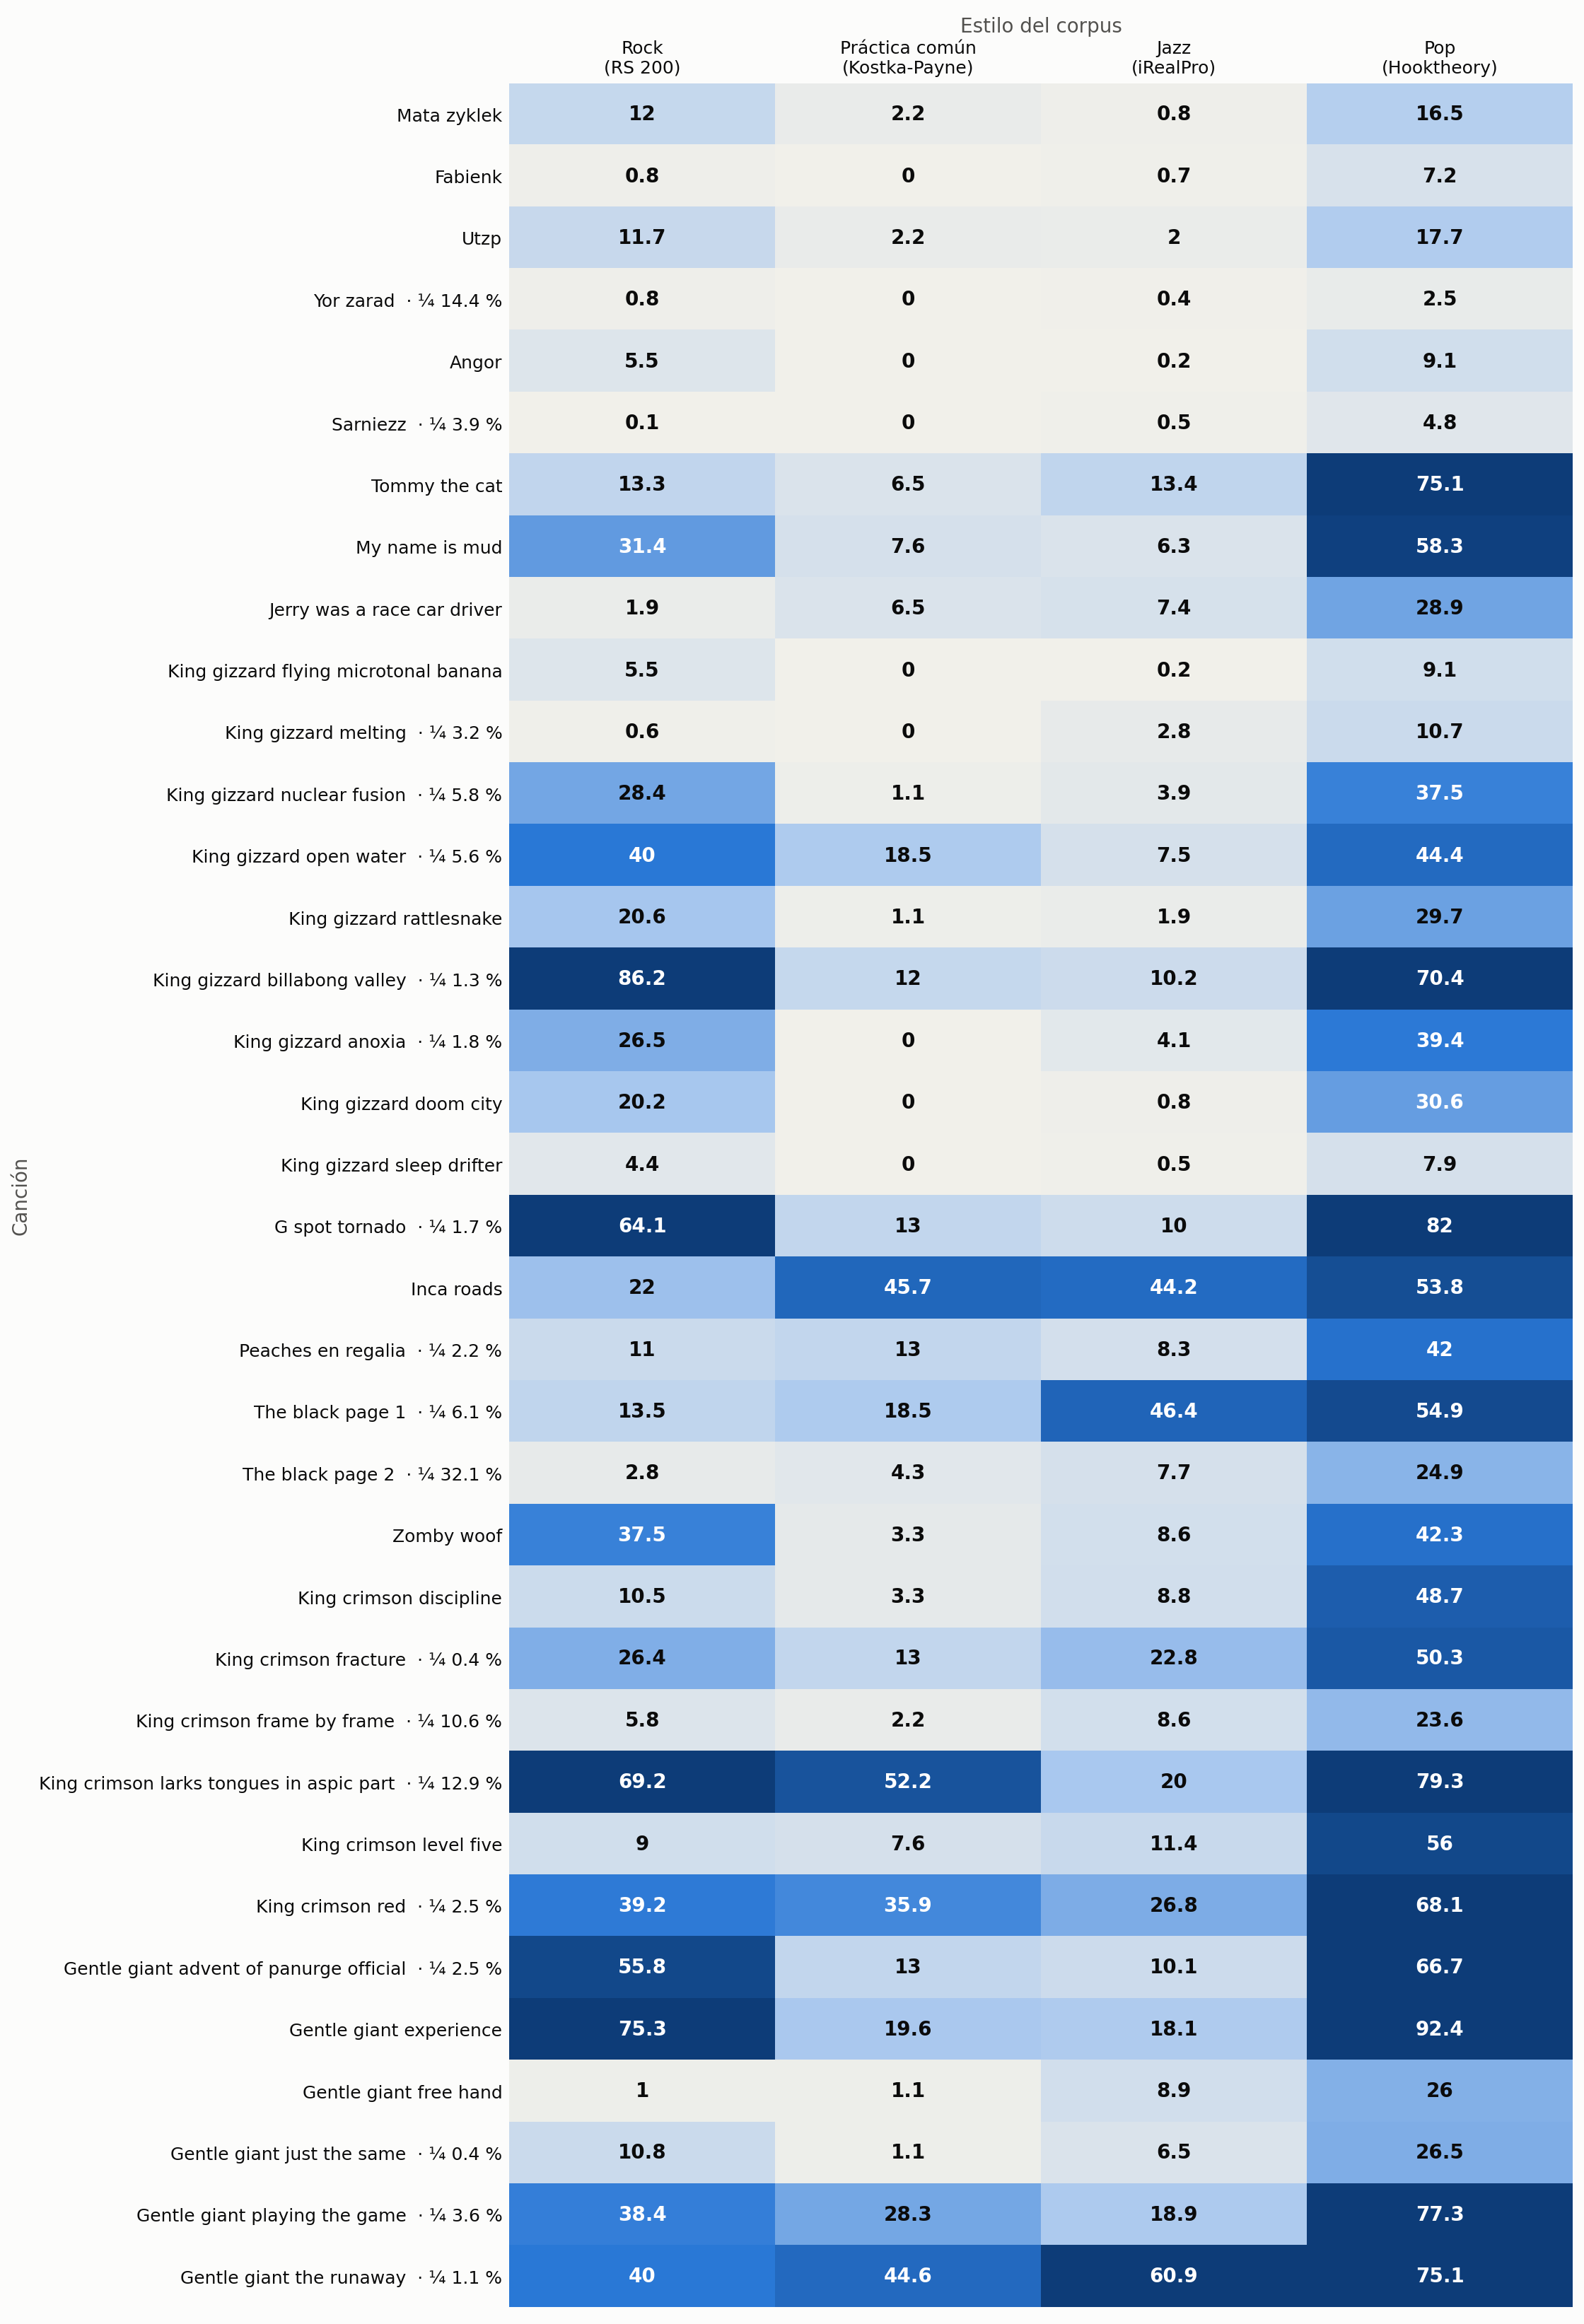
\includegraphics[width=\textwidth,height=0.78\textheight,keepaspectratio]{g_verosimilitud_matriz.png}
  \caption{Matriz de verosimilitud armónica de las 36 canciones frente a rock (RS~200, de Clercq y Temperley), práctica común (Kostka-Payne), jazz (iRealPro) y pop (9 álbumes de Hooktheory). Percentil: porcentaje de piezas del estilo tan o más alejadas que la canción (50 = típica). «¼\,\%»: tiempo con fundamental en cuarto de tono, llevada al grado de abajo.}\label{fig:g-matriz}
\end{figure}

\begin{figure}[!htbp]
  \centering
  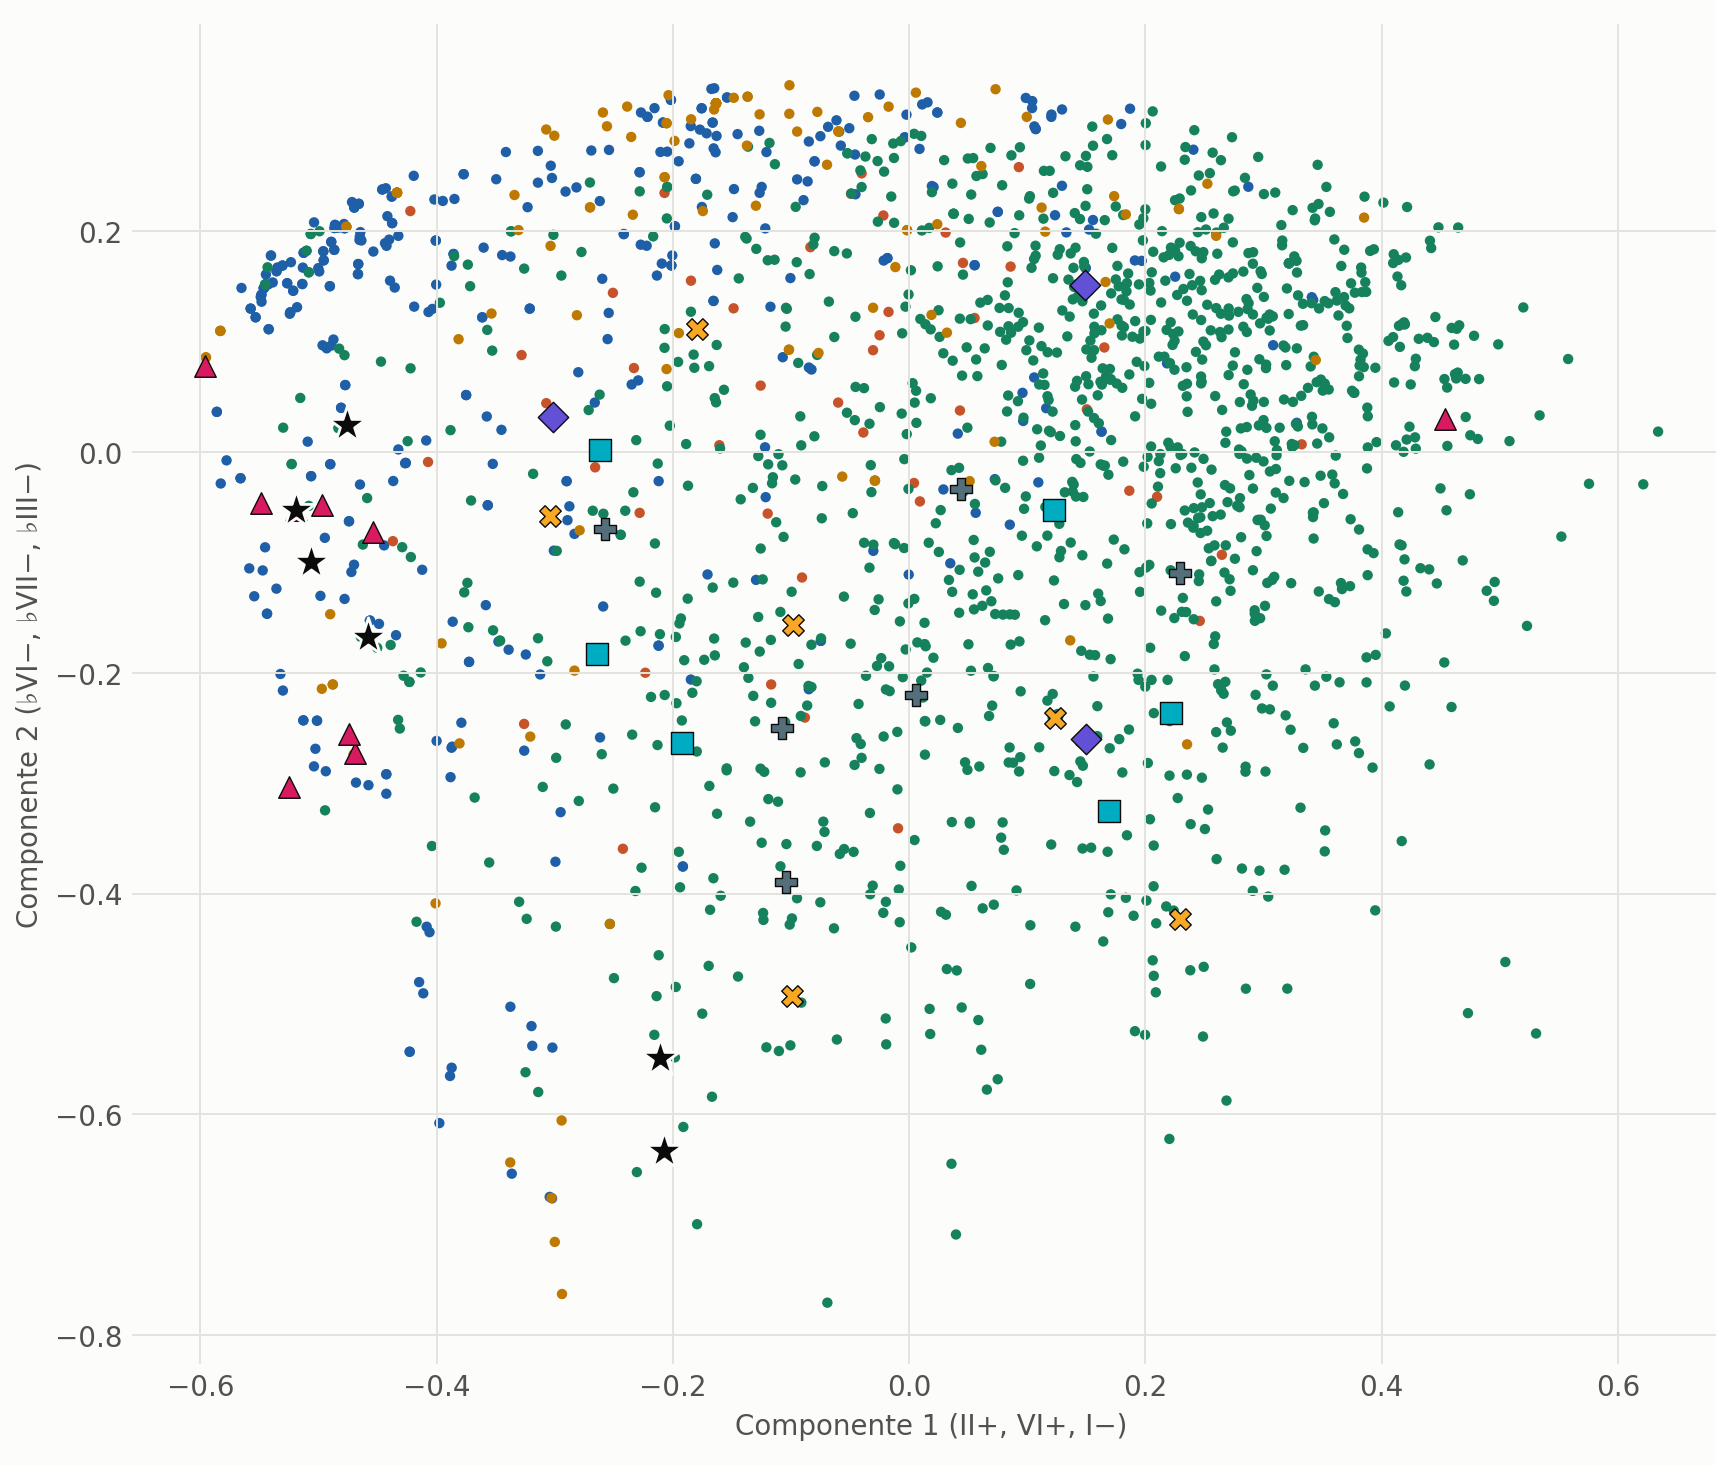
\includegraphics[width=\textwidth]{g_verosimilitud_mapa.png}
  \caption{Mapa de fundamentales de las 36 canciones. Puntos del fondo: rock (azul, RS~200, 400 piezas), práctica común (rojo, Kostka-Payne, 46), jazz (verde, iRealPro, 1186) y pop (naranja, Hooktheory, 121). Símbolos: estrella negra, la banda; rombo violeta, Primus; triángulo rosa, King Gizzard; cuadrado turquesa, Zappa; cruz gris, King Crimson; aspa amarilla, Gentle Giant.}
  \label{fig:g-mapa}
\end{figure}

\begin{figure}[!htbp]
  \centering
  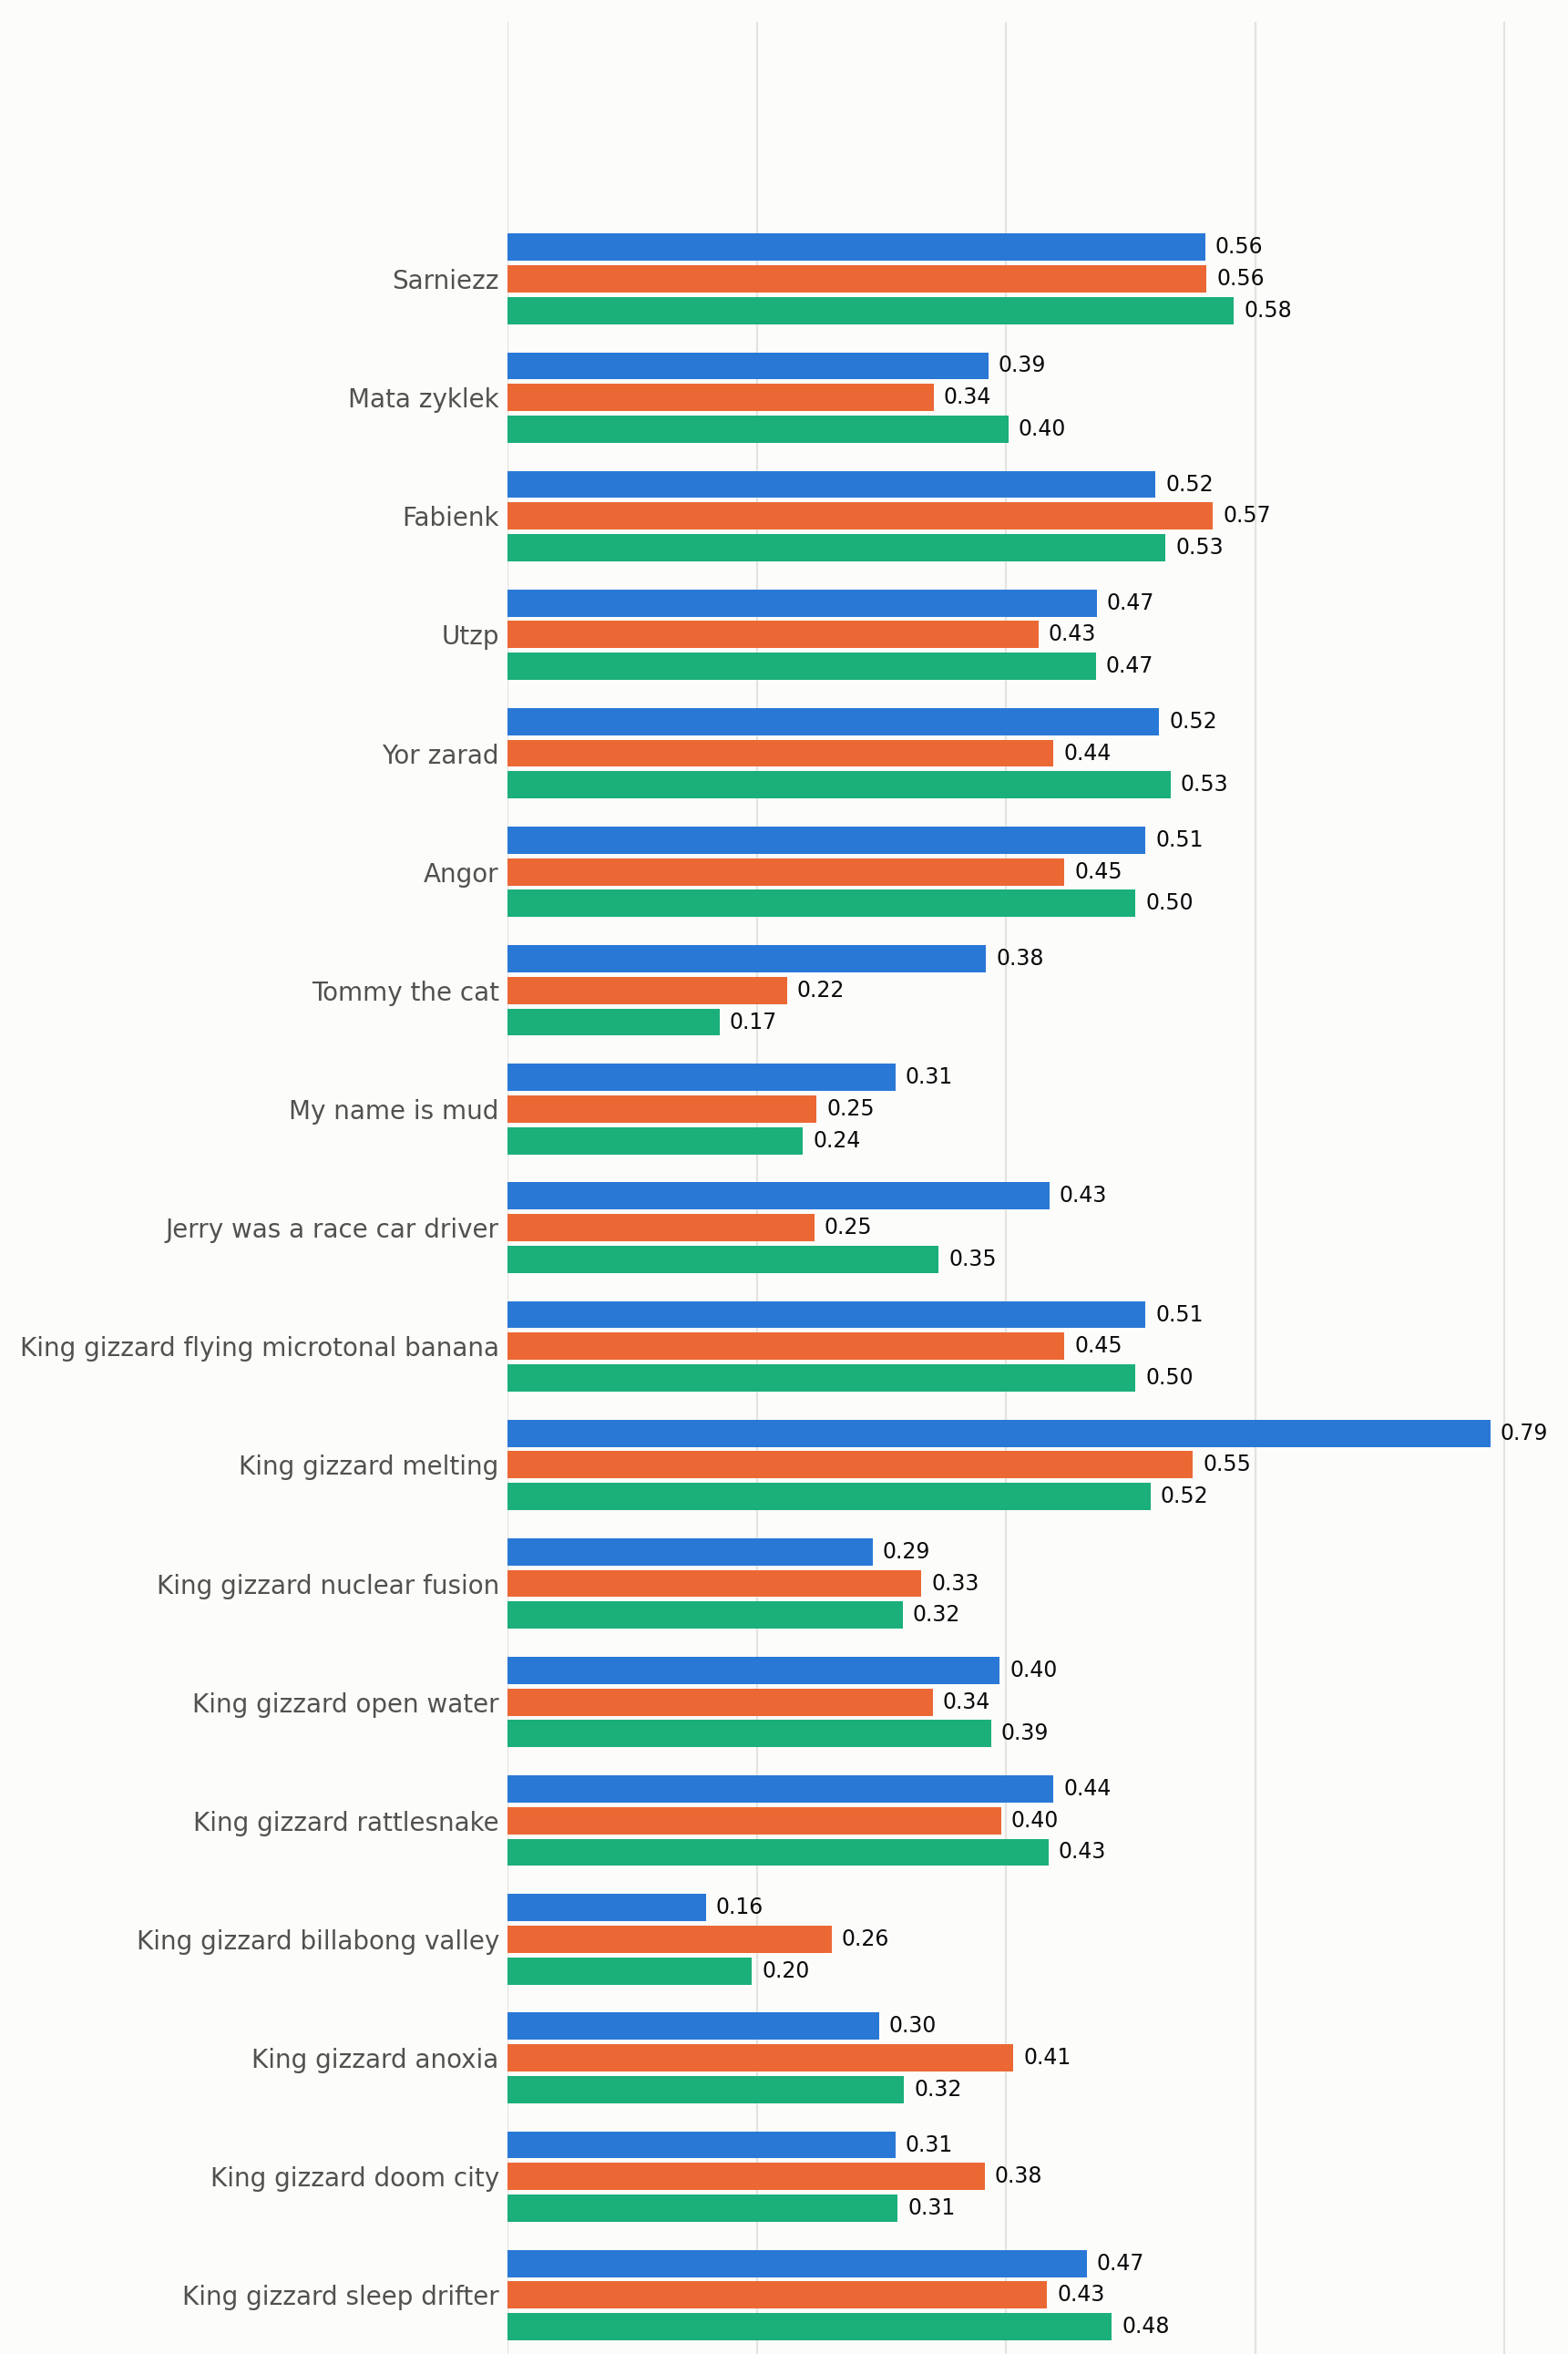
\includegraphics[width=0.495\textwidth]{g_distancias_estilos_a.png}\hfill
  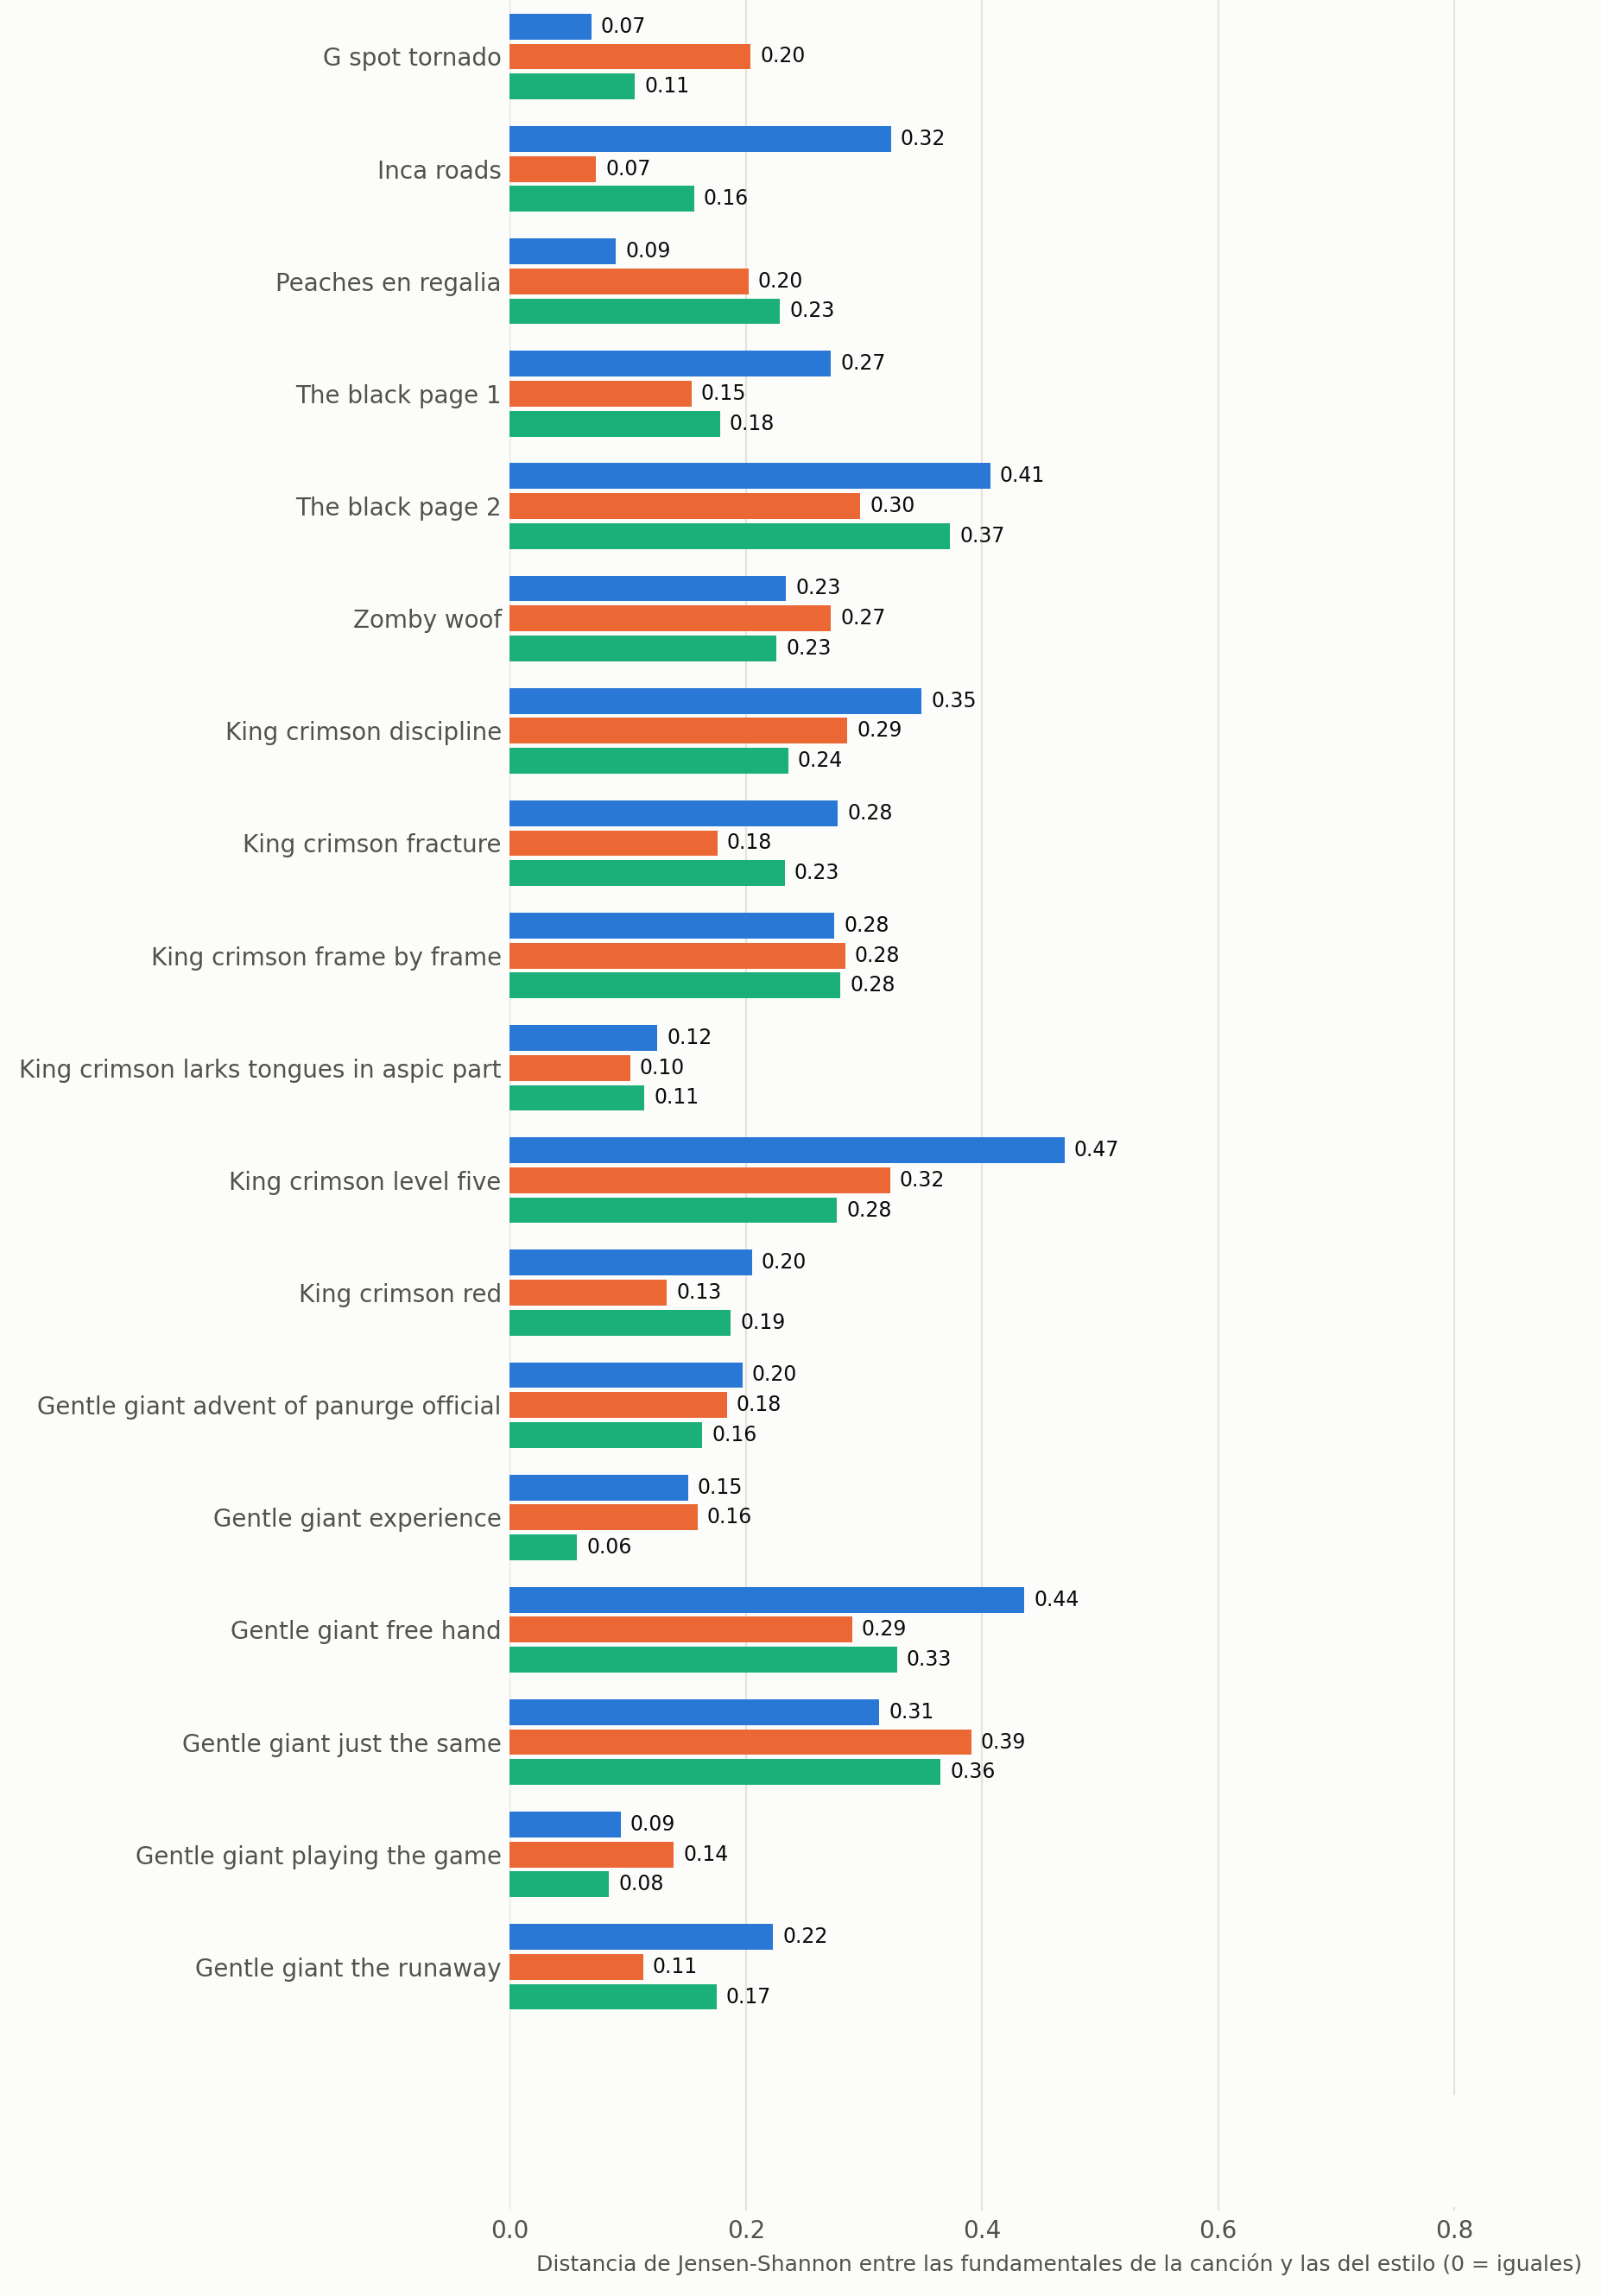
\includegraphics[width=0.495\textwidth]{g_distancias_estilos_b.png}
  \caption{Distancia de Jensen-Shannon de las fundamentales de cada canción a rock (azul, 100 canciones), práctica común (naranja) y pop (verde, 9 álbumes); 0 = iguales. Las canciones siguen en la columna derecha. Versión con reglas, descartada.}
  \label{fig:g-distancias}
\end{figure}

\begin{figure}[!htbp]
  \centering
  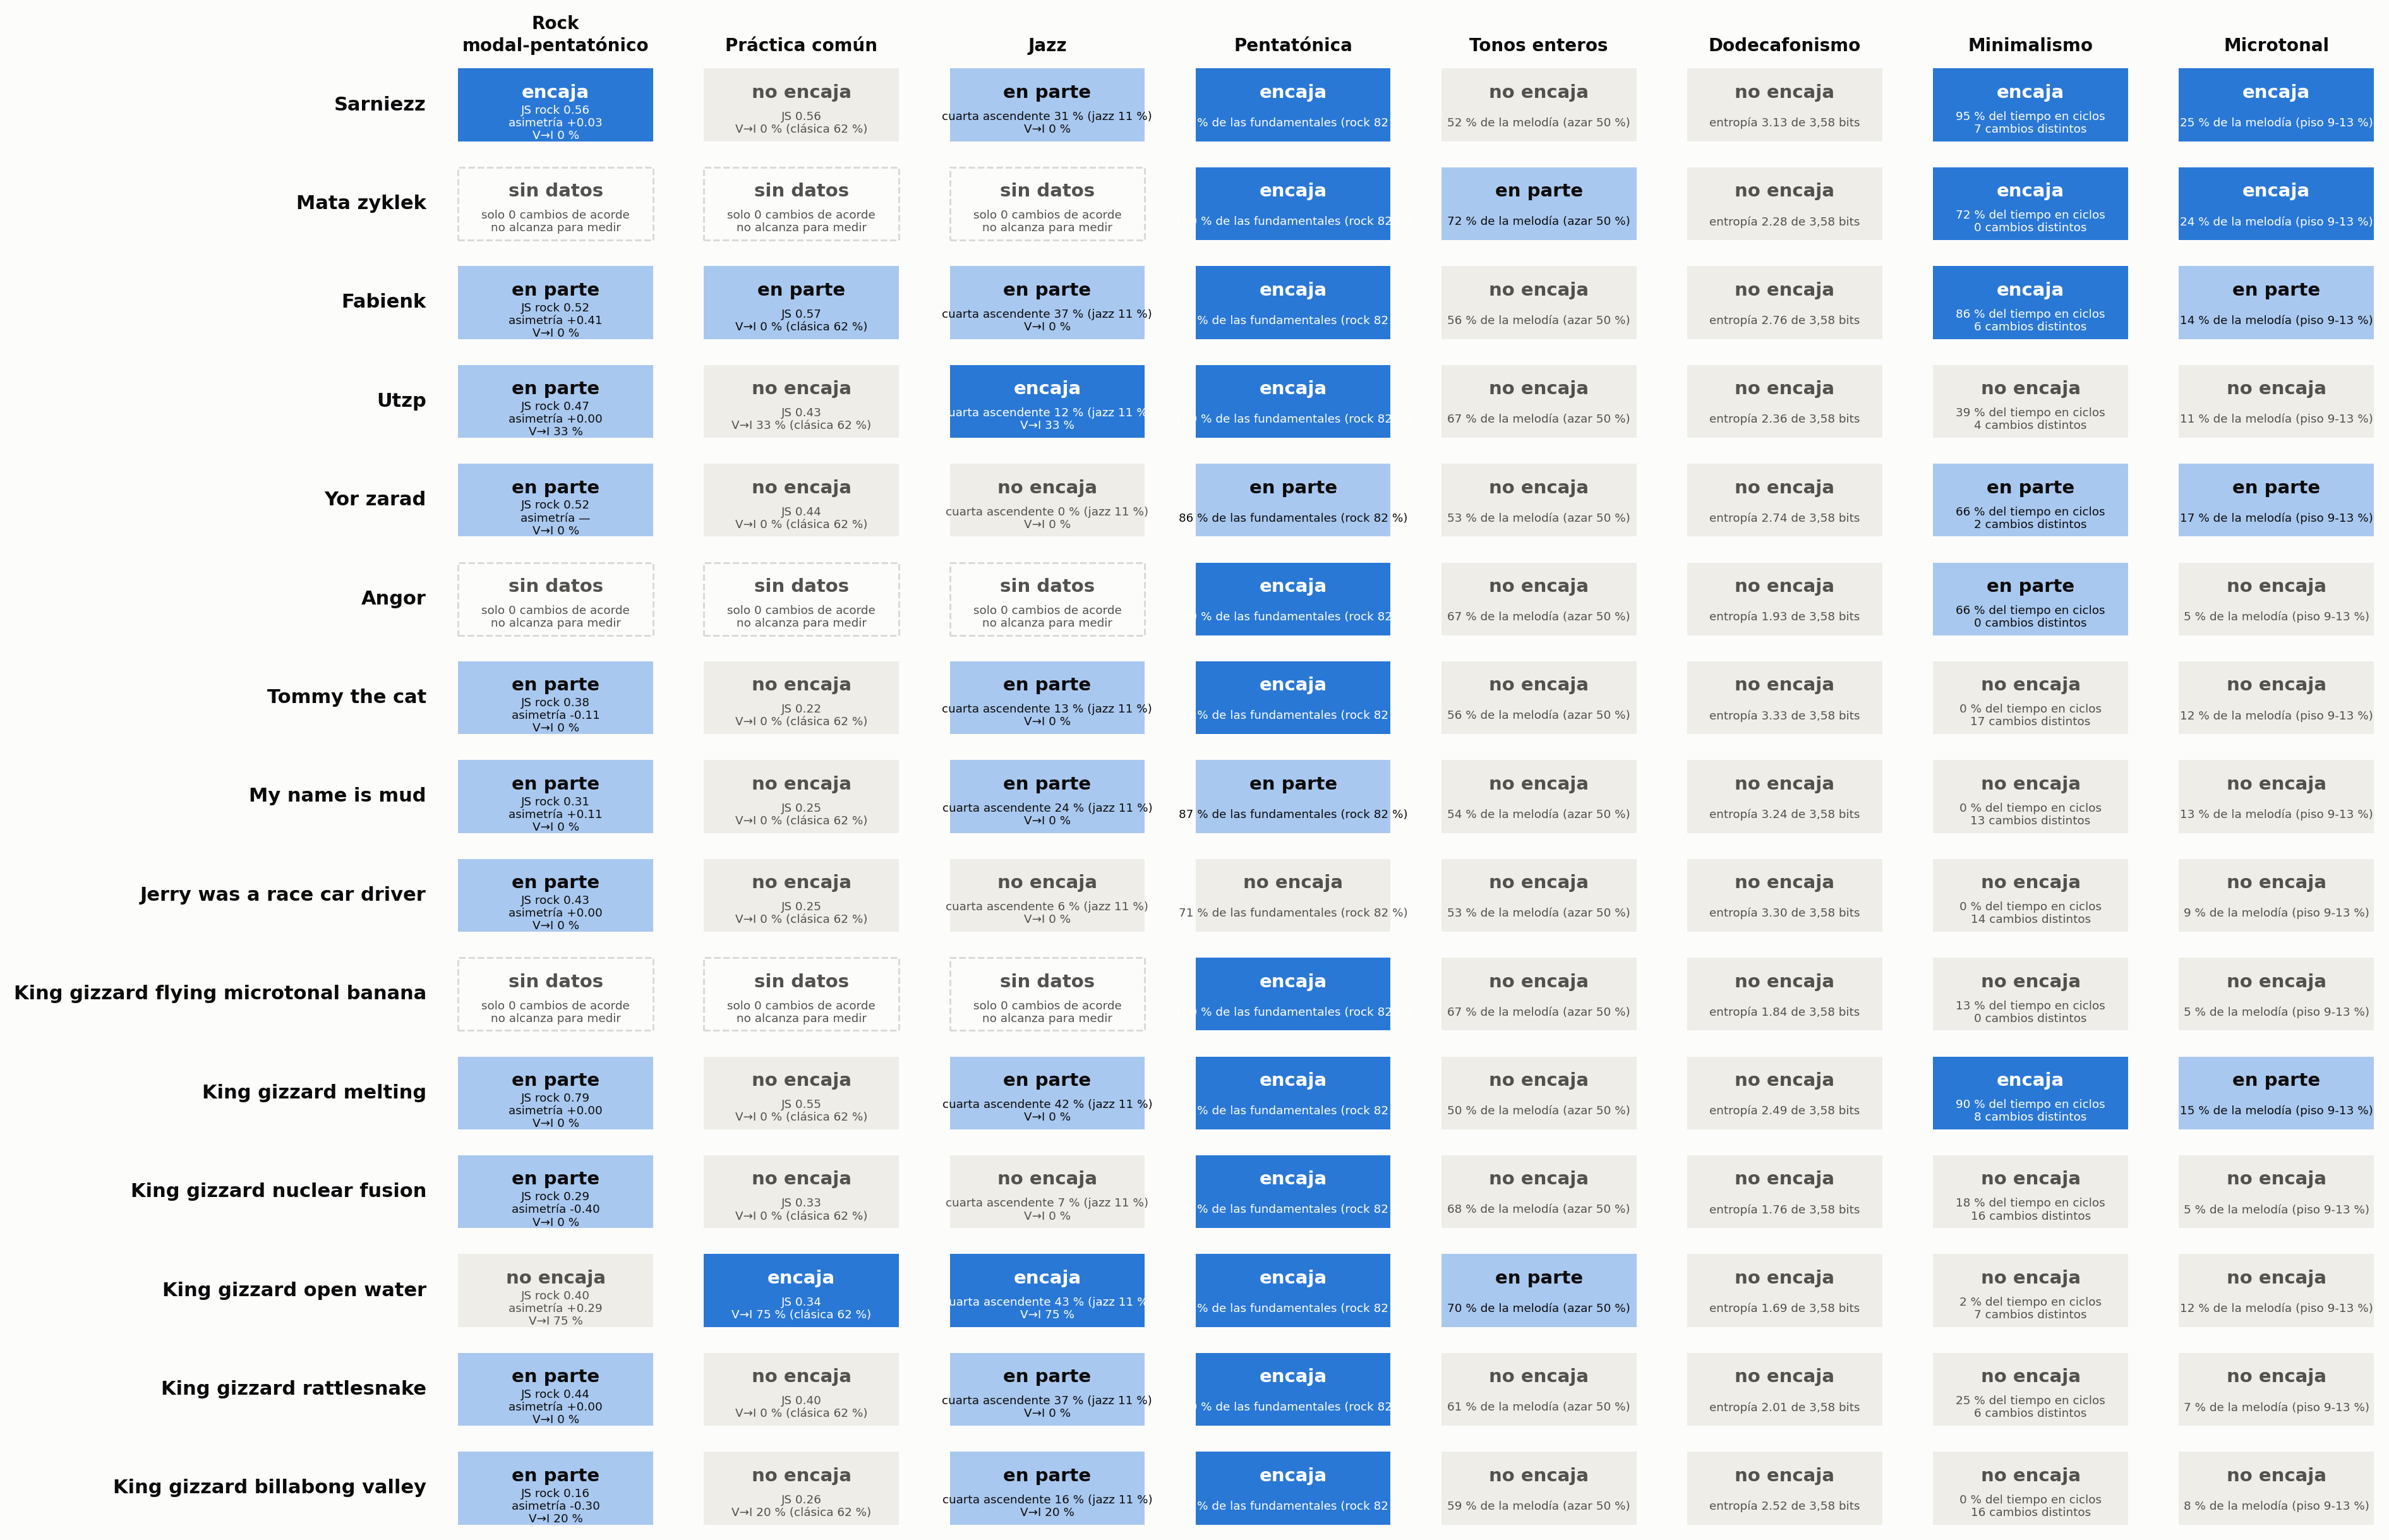
\includegraphics[width=\textwidth,height=0.78\textheight,keepaspectratio]{g_veredictos_estilos_1.png}
  \caption{Pruebas de estilo con reglas, canciones 1--15 (versión descartada). Azul oscuro: encaja; azul claro: encaja en parte; gris: no encaja; blanco: sin datos.}\label{fig:g-veredictos1}
\end{figure}

\begin{figure}[!htbp]
  \centering
  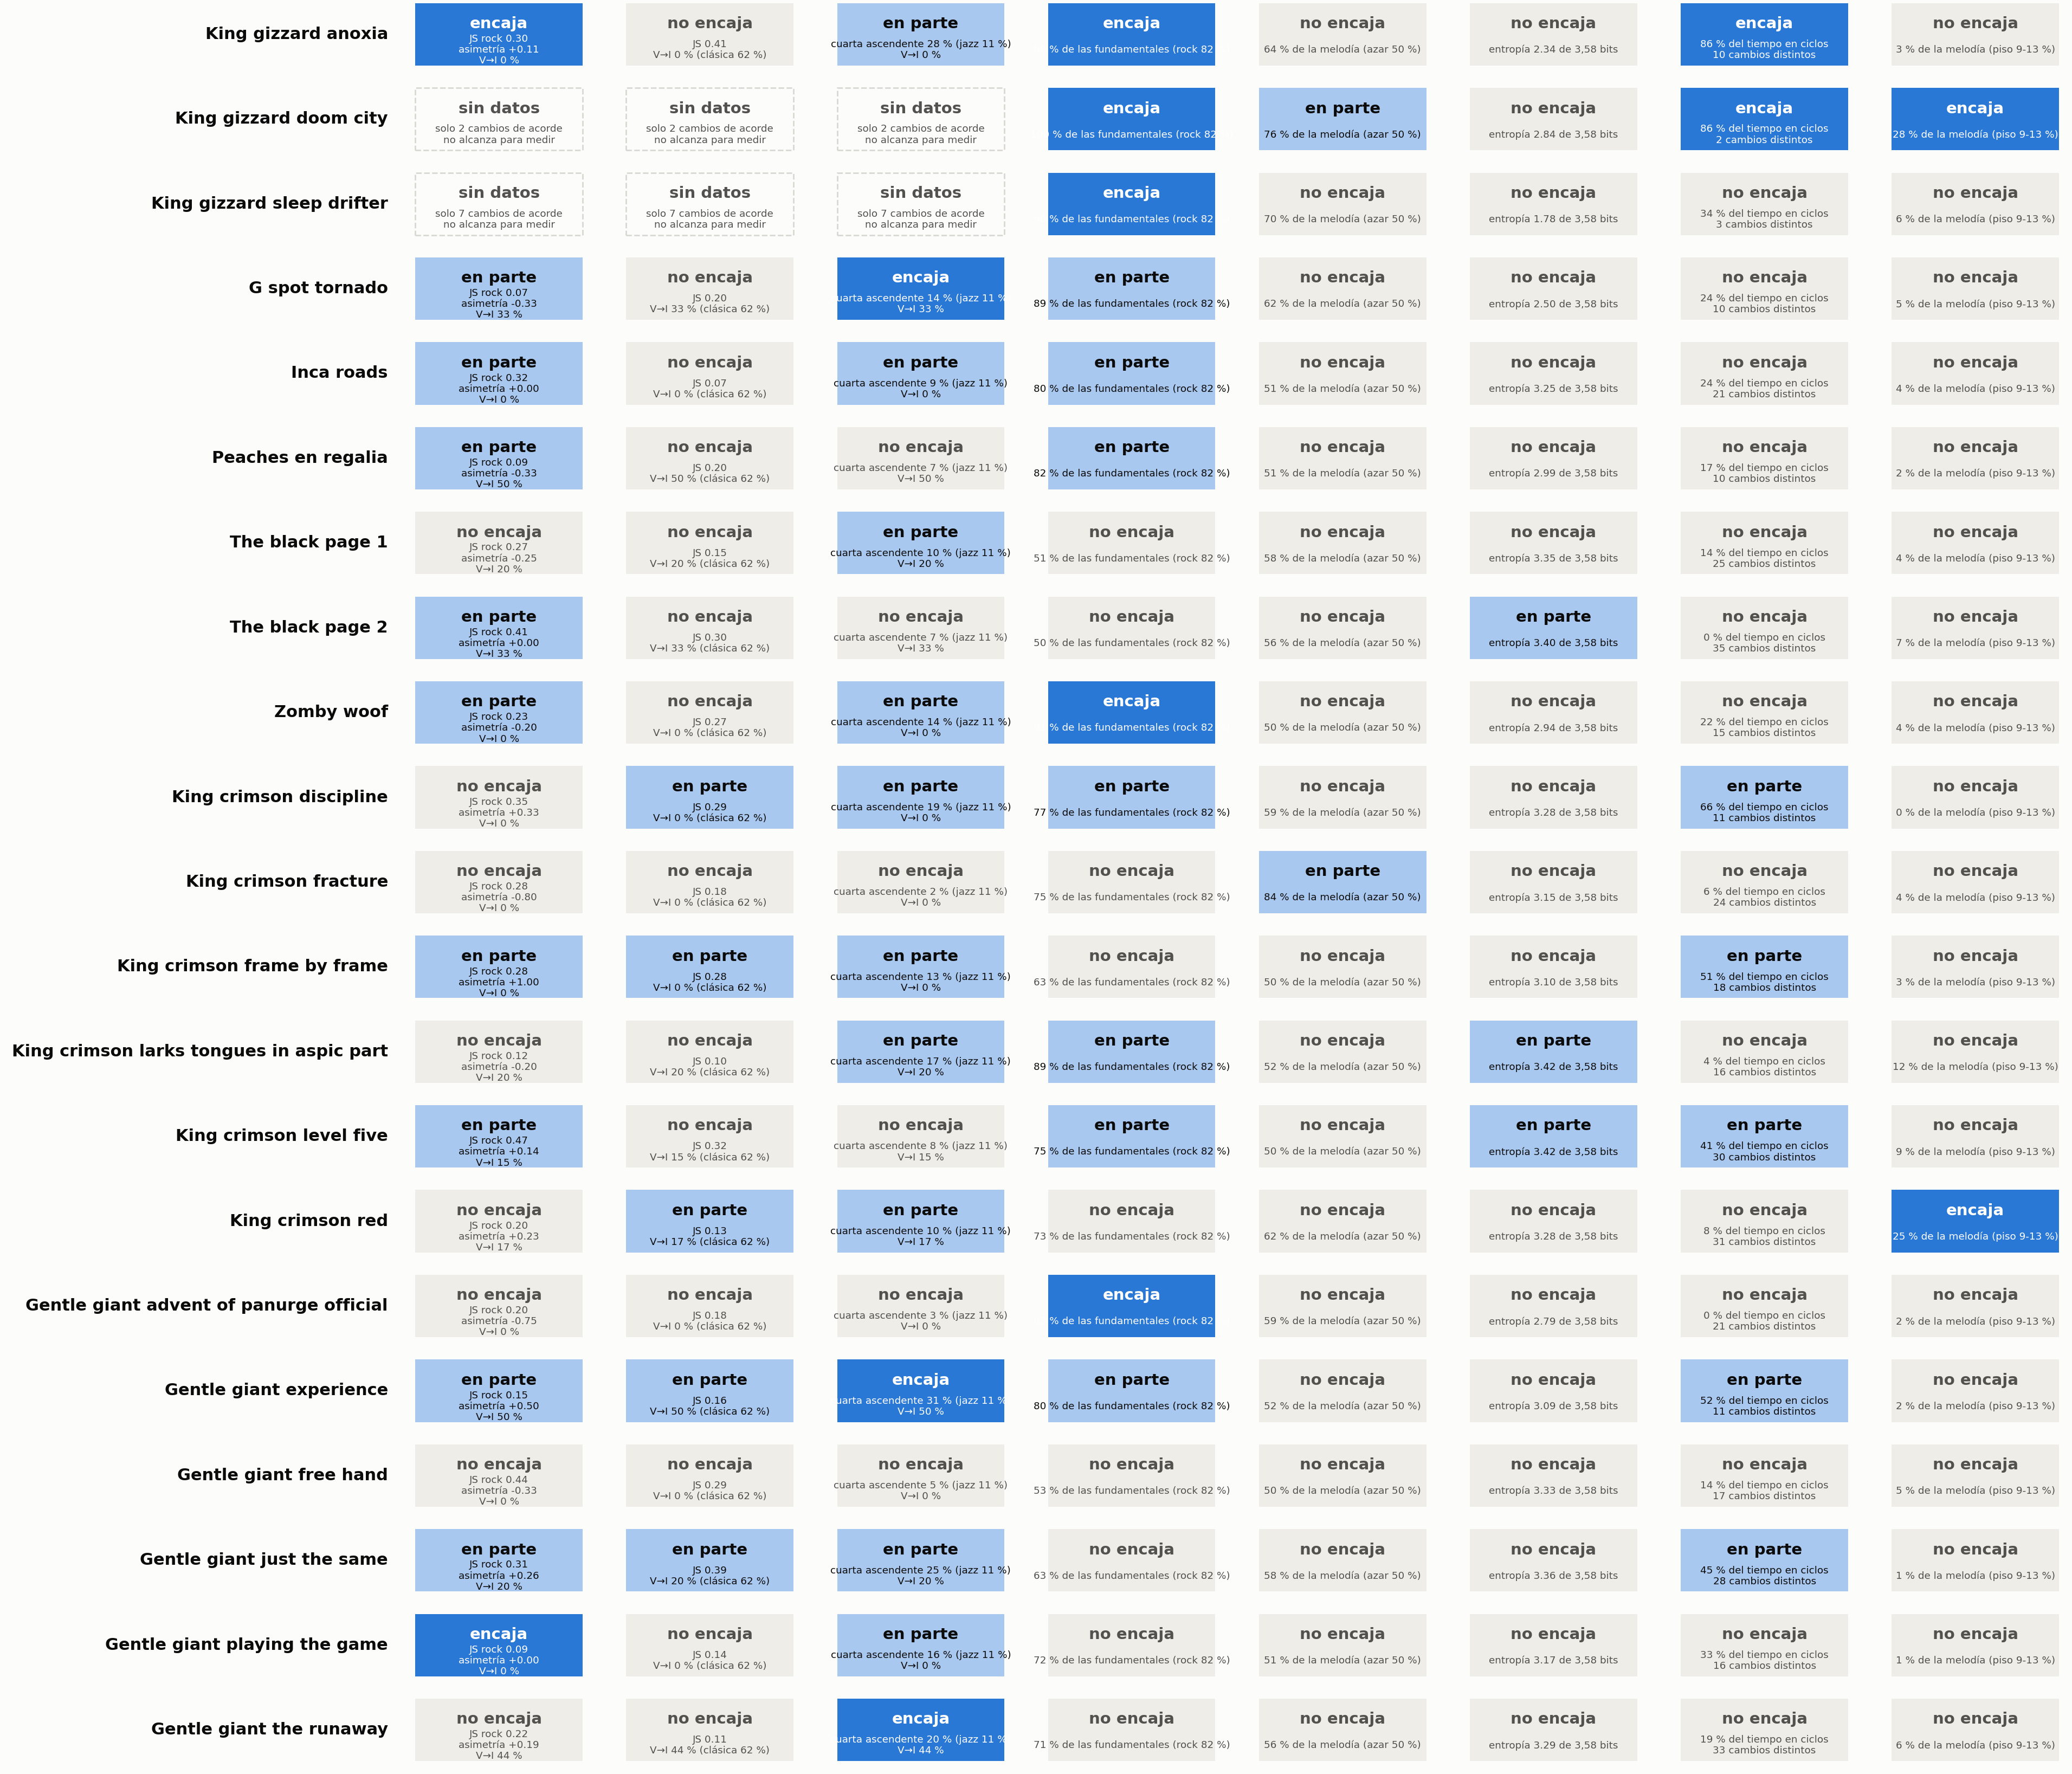
\includegraphics[width=\textwidth,height=0.78\textheight,keepaspectratio]{g_veredictos_estilos_2.png}
  \caption{Pruebas de estilo con reglas, canciones 16--36; misma lectura que la figura~\ref{fig:g-veredictos1}.}\label{fig:g-veredictos2}
\end{figure}

\section{Melodía}

La figura~\ref{fig:g-uso} amplía la figura~\ref{fig:uso} a las 36 canciones, y las figuras~\ref{fig:g-escalas1} y~\ref{fig:g-escalas2} muestran la escala de cada una.

\begin{figure}[!htbp]
  \centering
  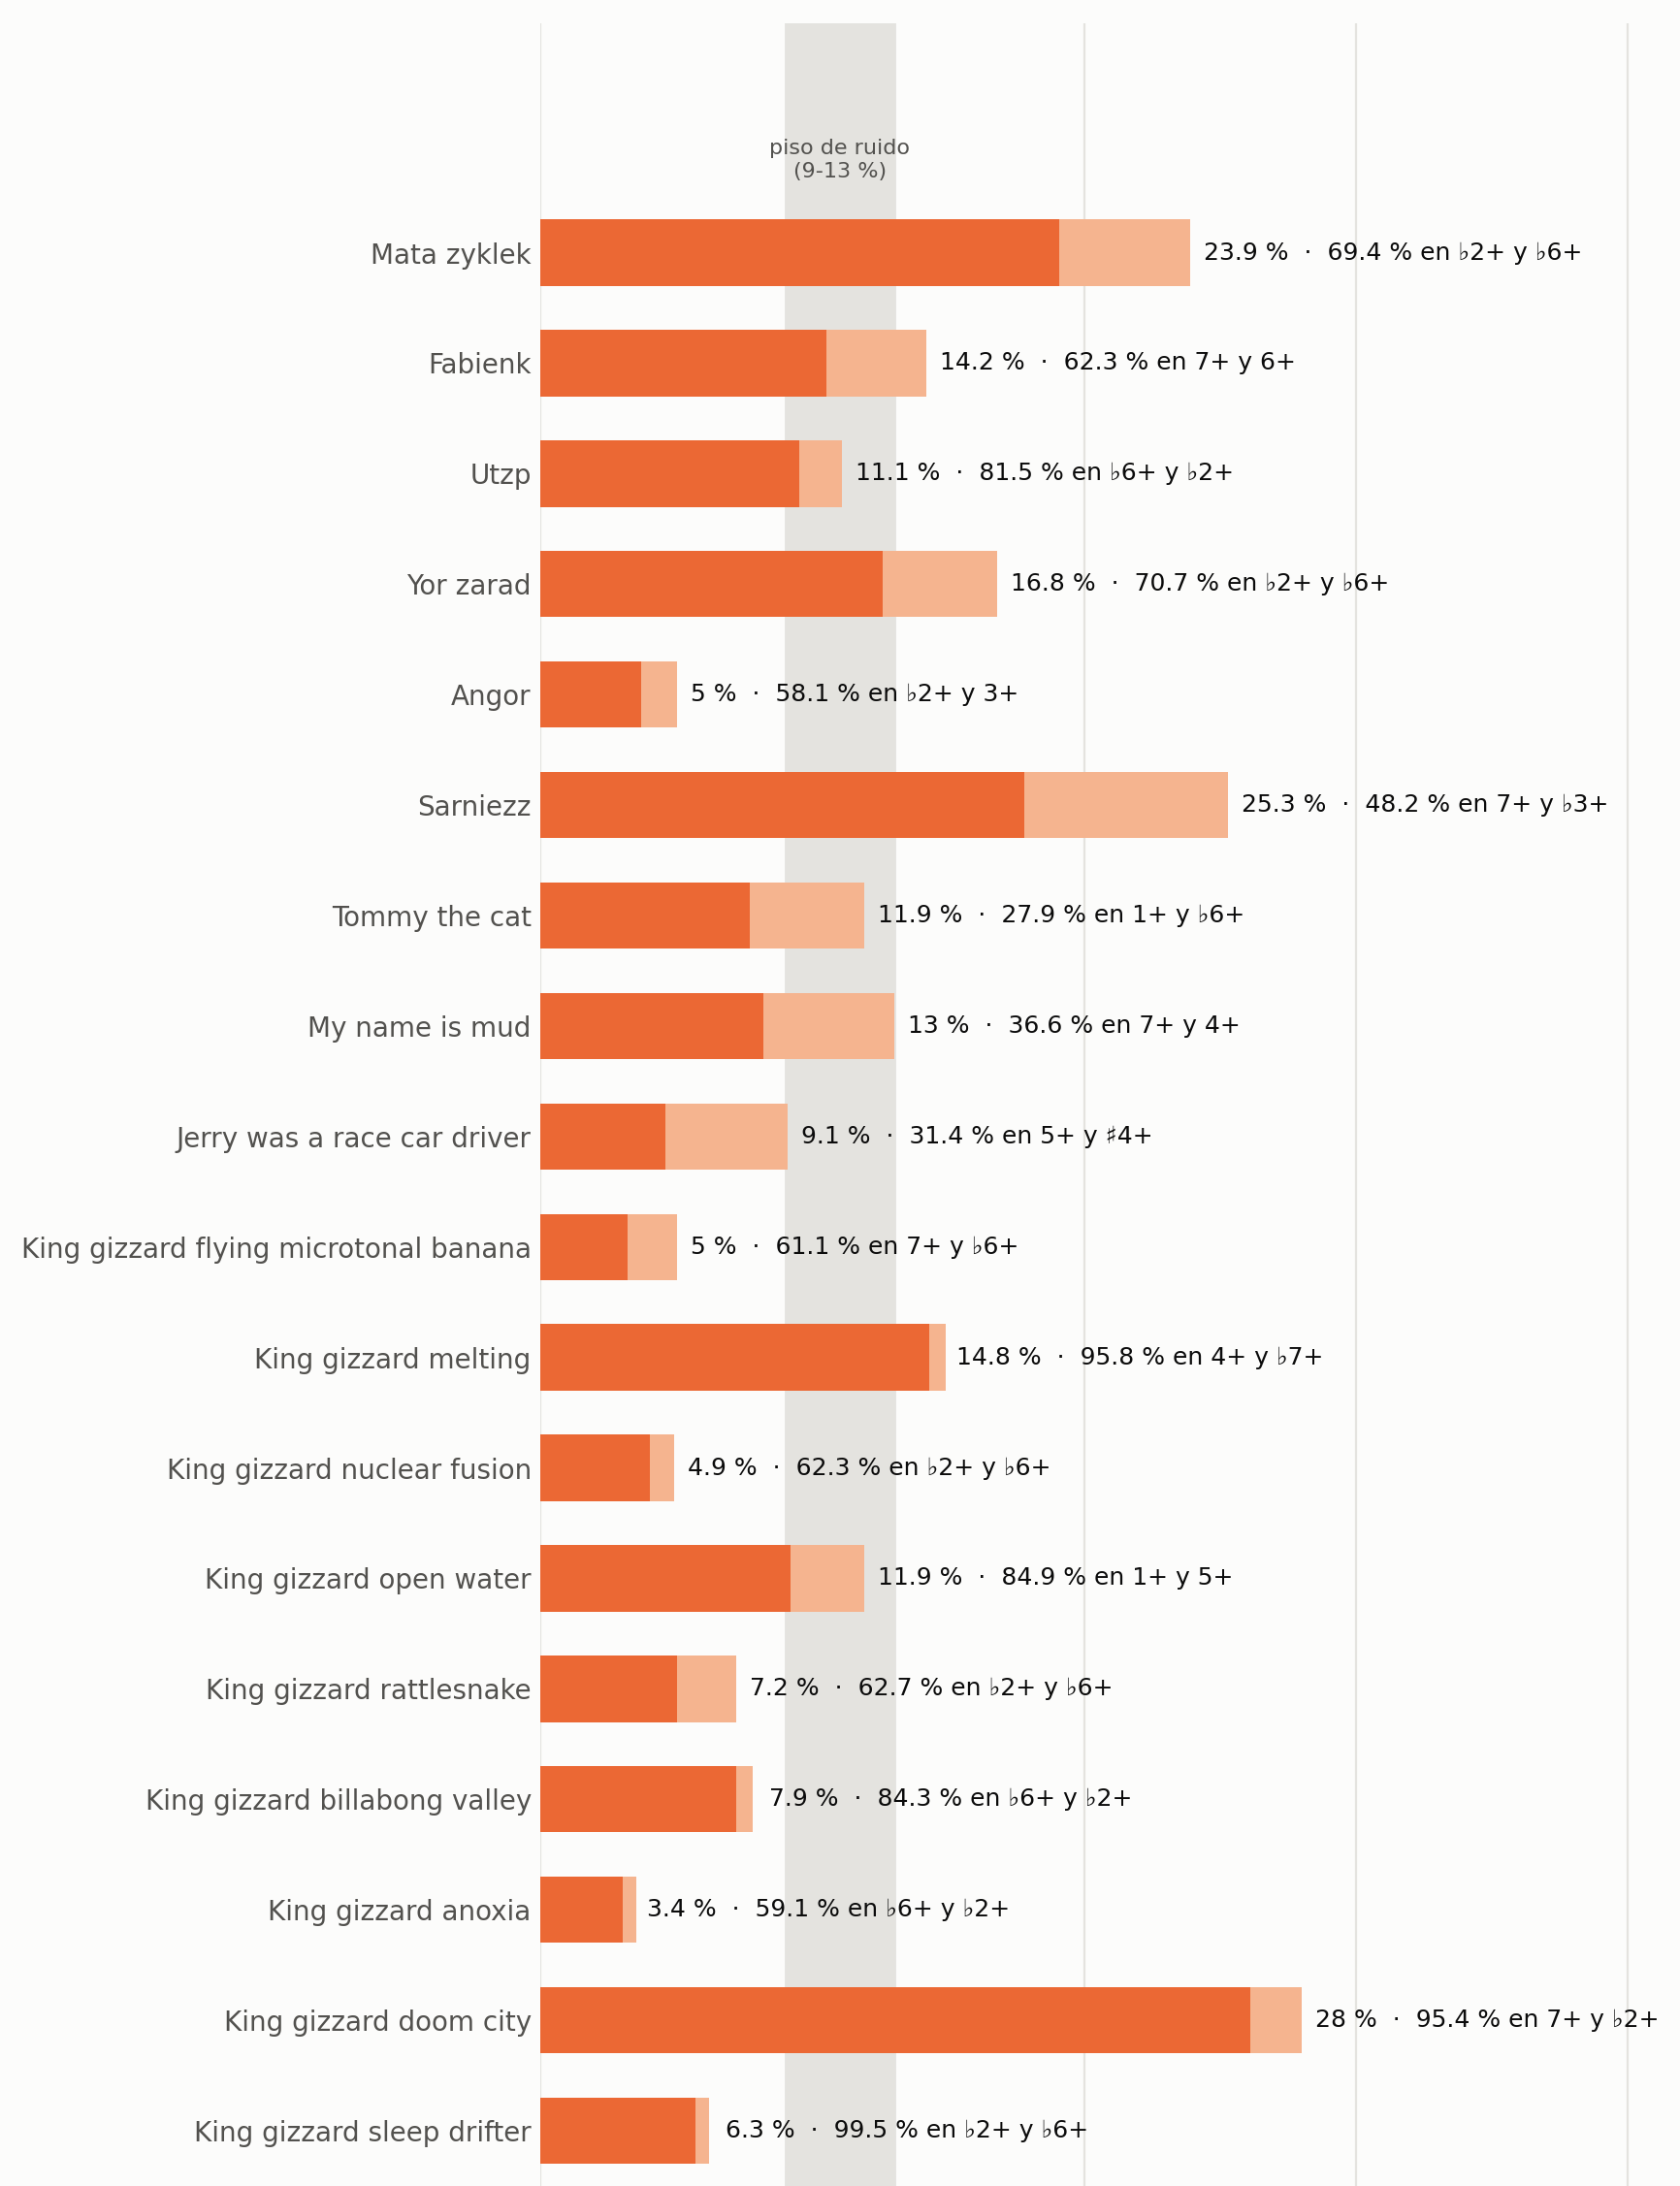
\includegraphics[width=0.495\textwidth]{g_microtonal_uso_a.png}\hfill
  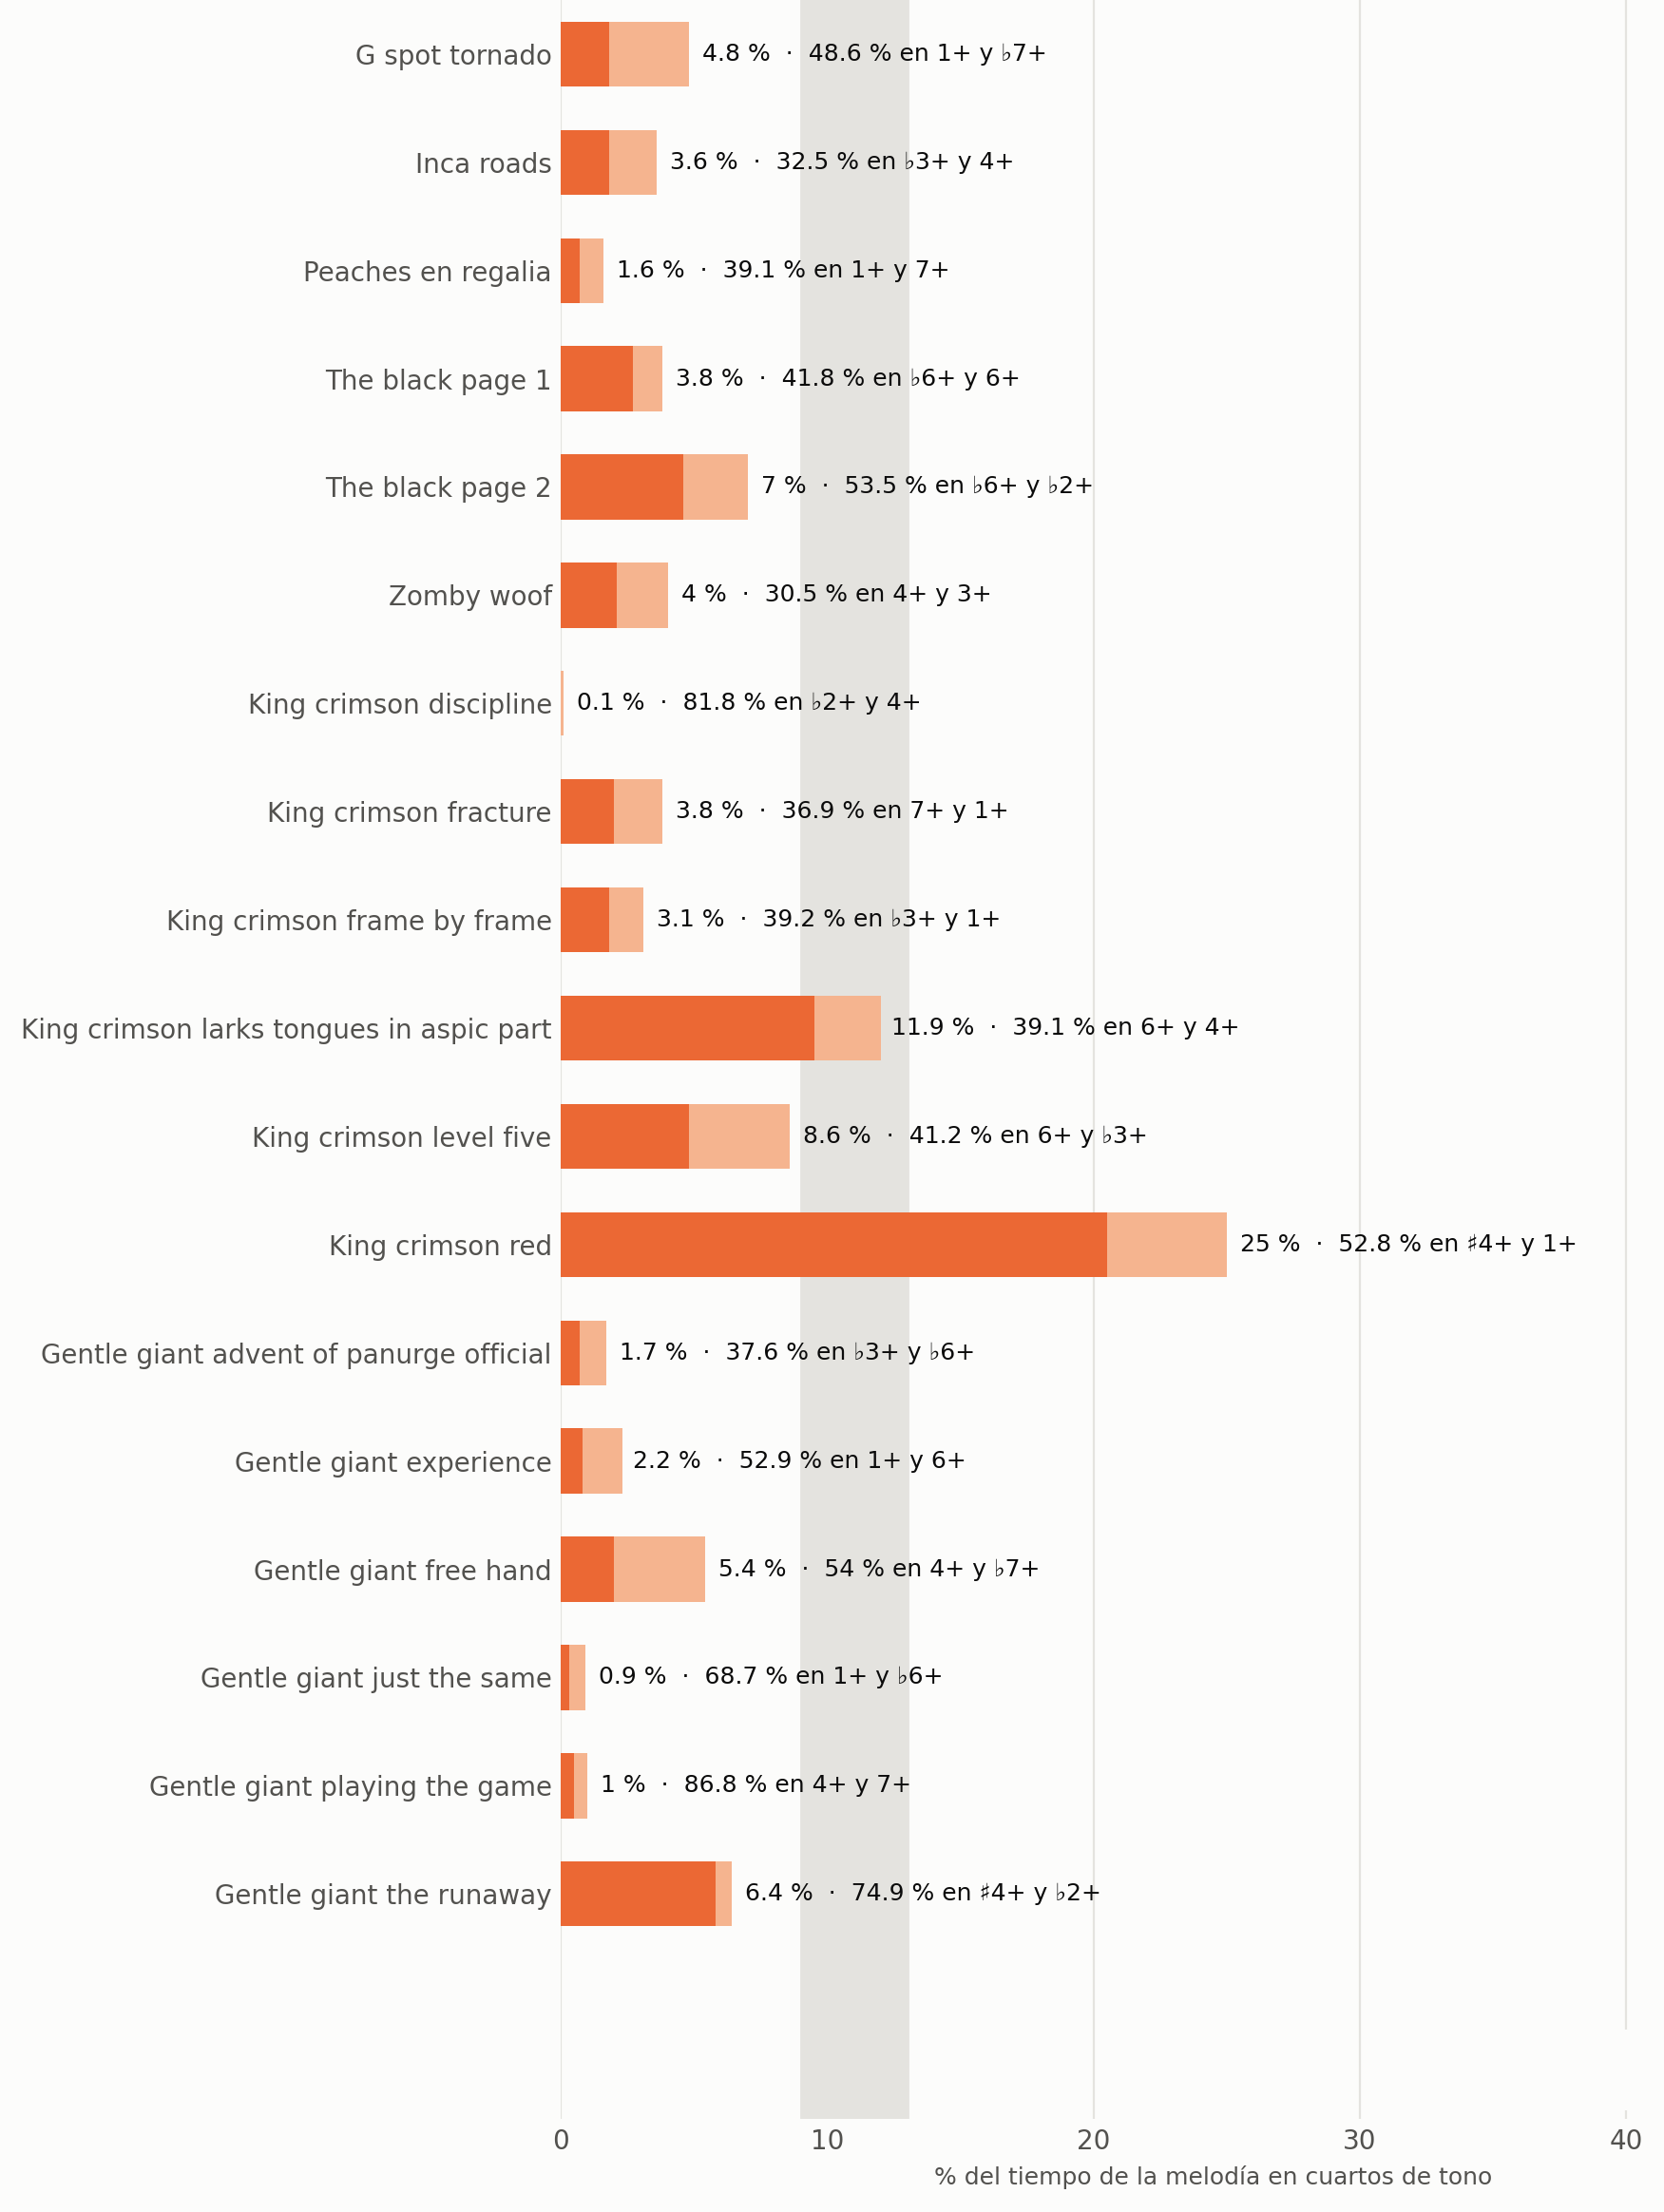
\includegraphics[width=0.495\textwidth]{g_microtonal_uso_b.png}
  \caption{Cuartos de tono en la melodía de las 36 canciones. Naranja oscuro: como grado; claro: como adorno; franja gris: piso de ruido (9--13\,\%). Junto a cada barra, el total y la fracción en los dos grados más usados. Las canciones siguen en la columna derecha.}\label{fig:g-uso}
\end{figure}

\begin{figure}[!htbp]
  \centering
  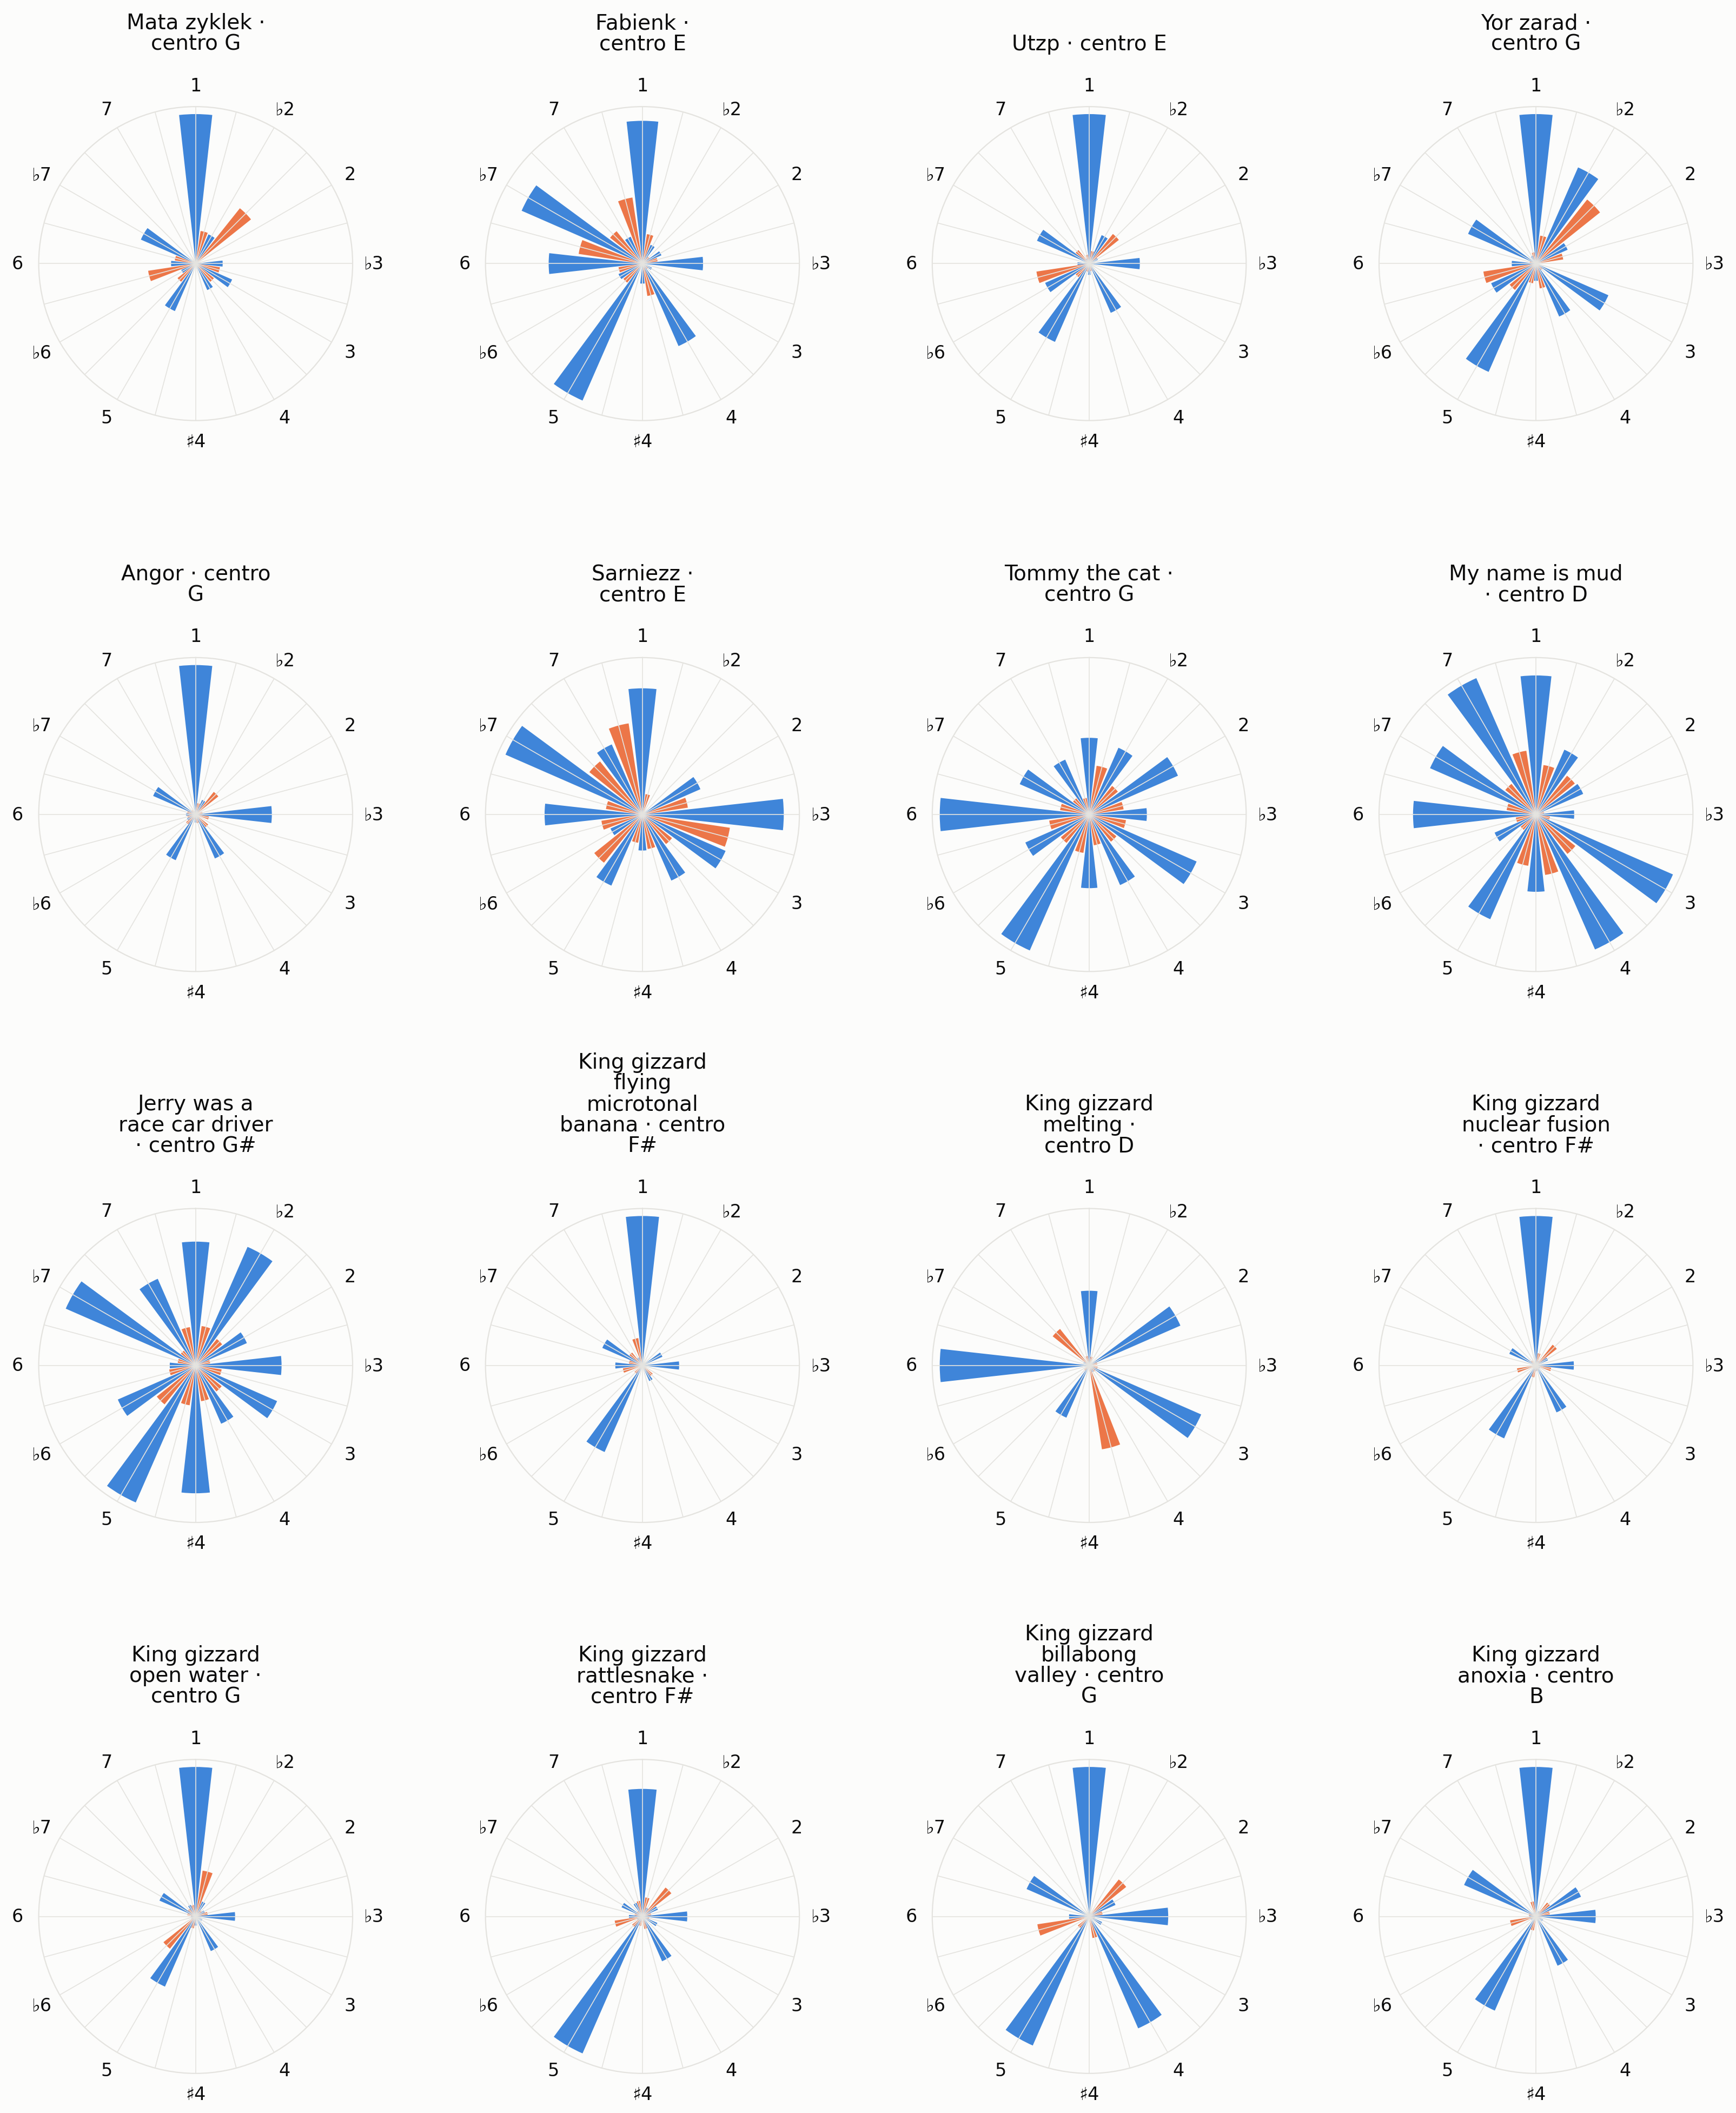
\includegraphics[width=\textwidth,height=0.78\textheight,keepaspectratio]{g_microtonal_escalas_1.png}
  \caption{Escala de cada canción en 24-EDO respecto de su centro (I). Largo del pétalo: tiempo en el grado; azul: grado regular; rojo: cuarto de tono.}\label{fig:g-escalas1}
\end{figure}

\begin{figure}[!htbp]
  \centering
  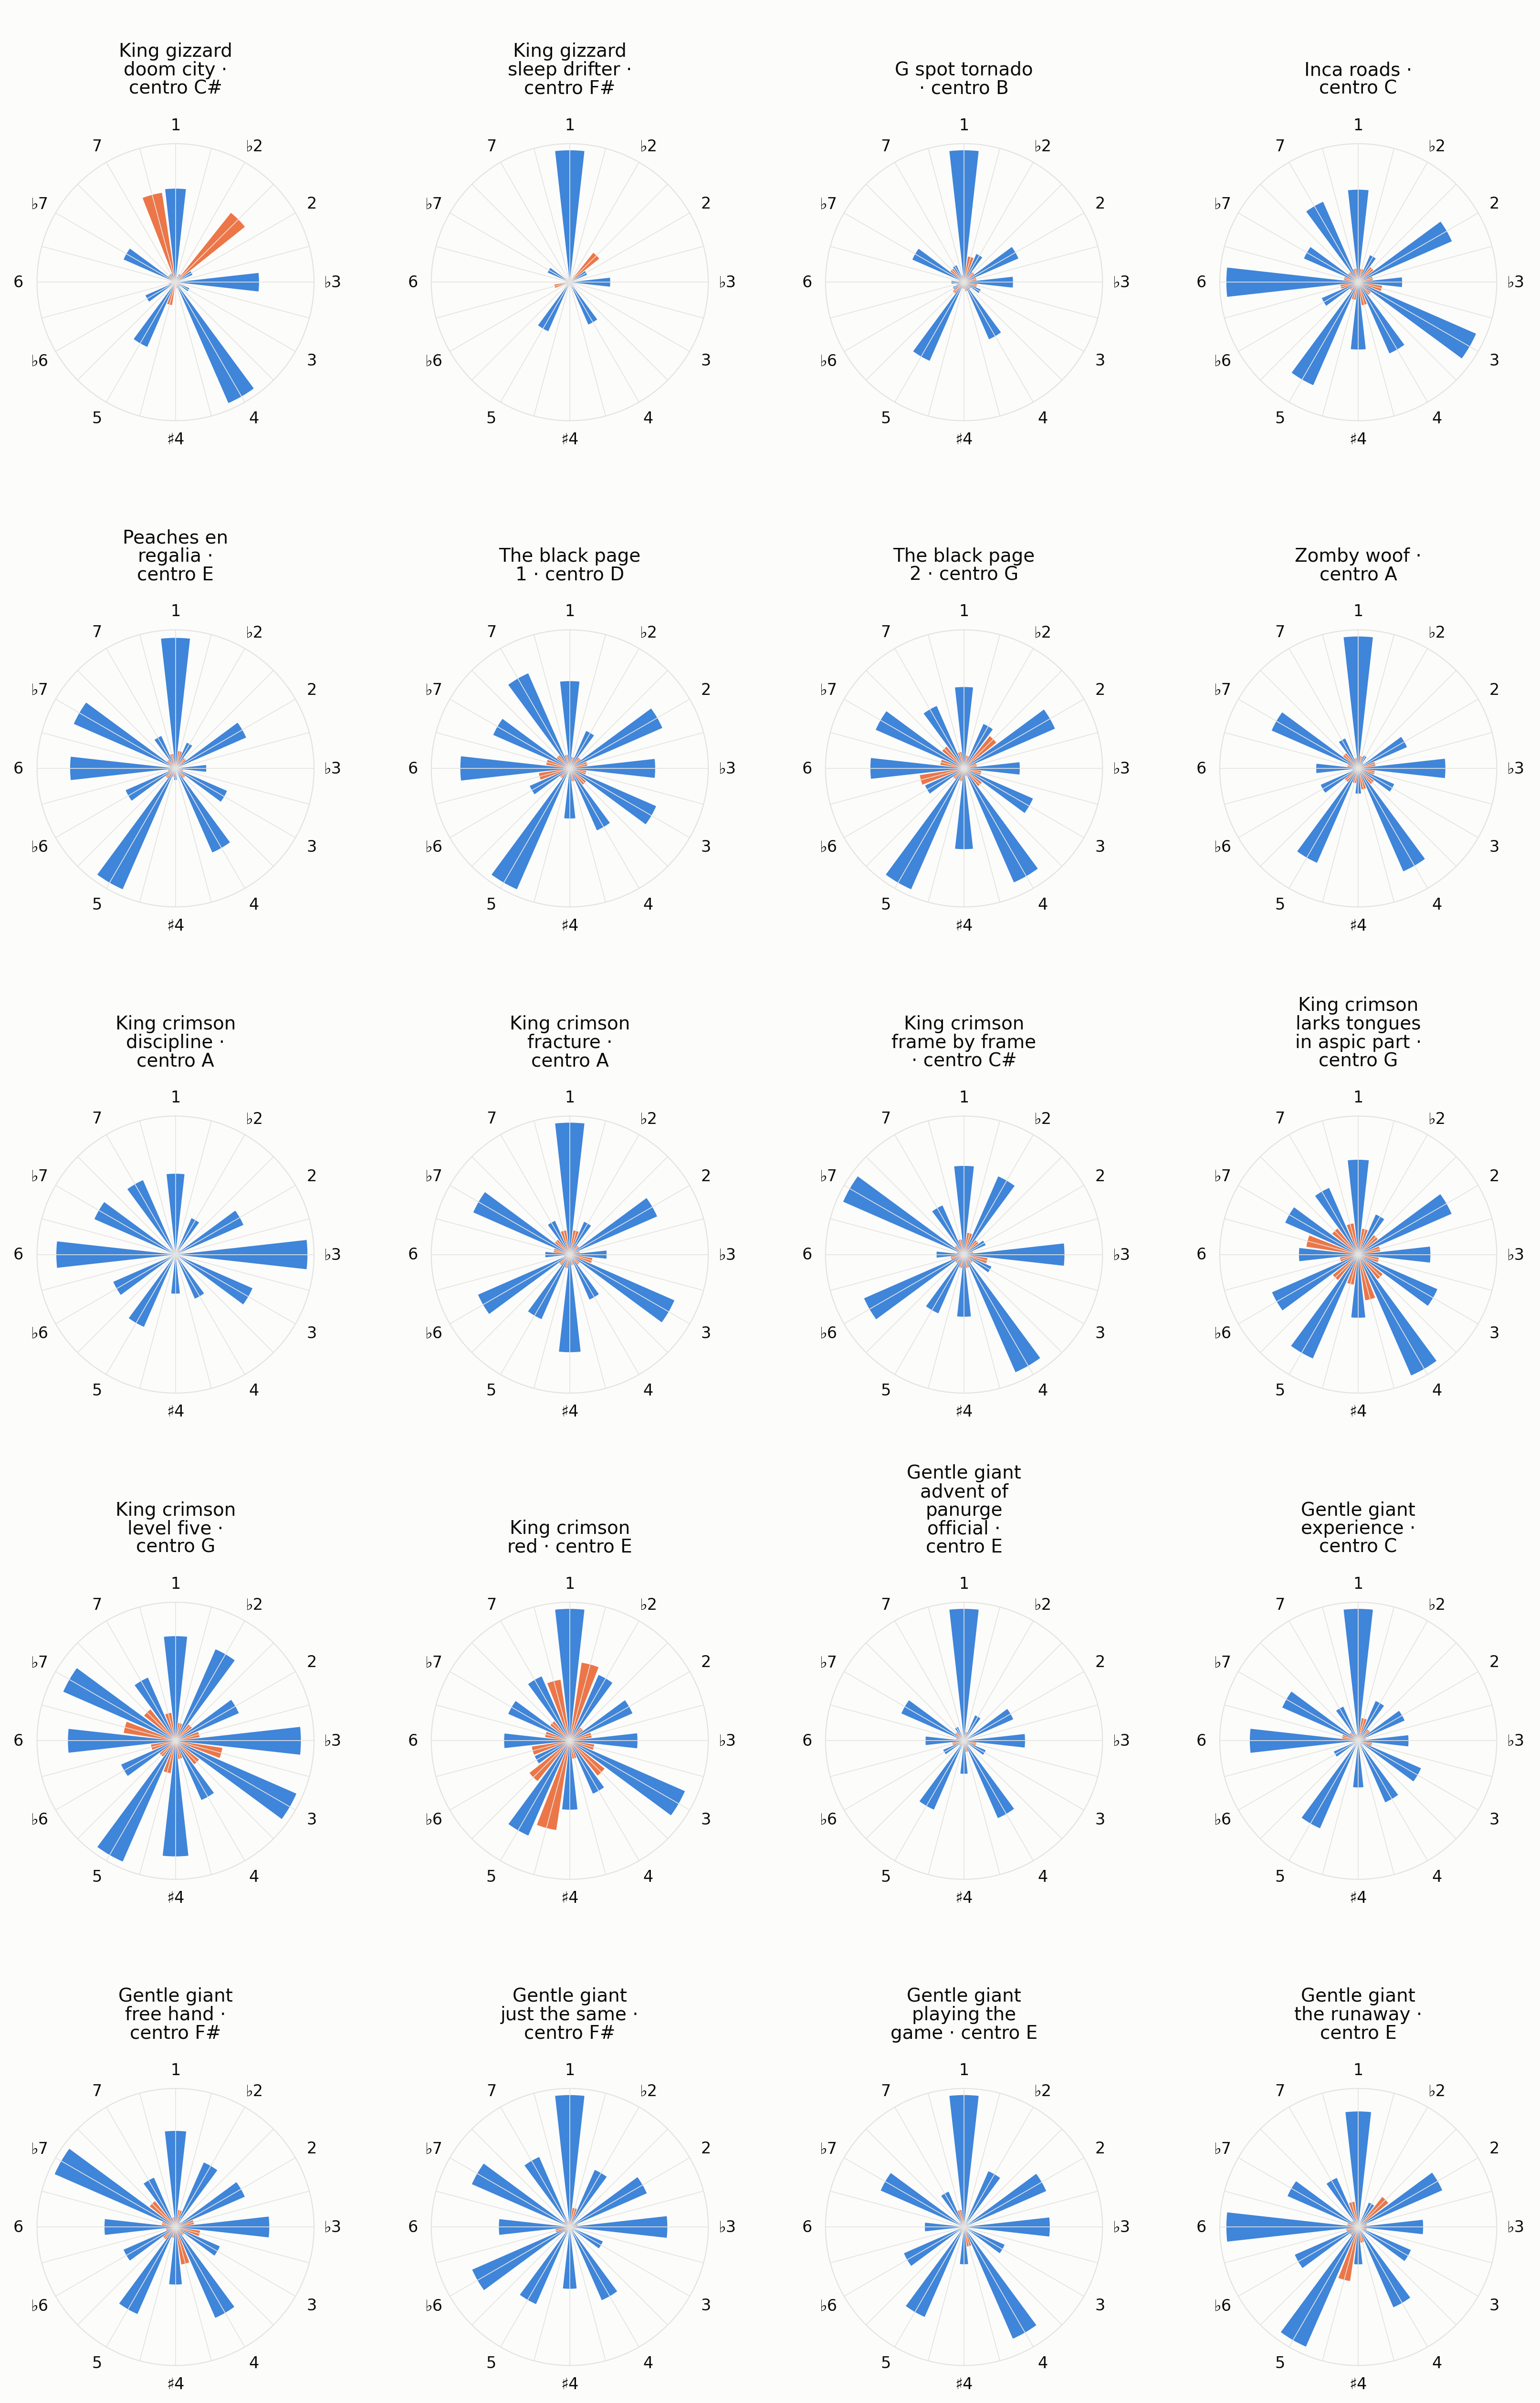
\includegraphics[width=\textwidth,height=0.78\textheight,keepaspectratio]{g_microtonal_escalas_2.png}
  \caption{Escala de cada canción en 24-EDO (II); misma lectura que la figura~\ref{fig:g-escalas1}.}\label{fig:g-escalas2}
\end{figure}

\section{Síntesis}

Las figuras~\ref{fig:g-bloques} y~\ref{fig:g-bloques-sintesis} dan el test por bloques completo (sección~\ref{sec:res-sintesis}).

\begin{figure}[!htbp]
  \centering
  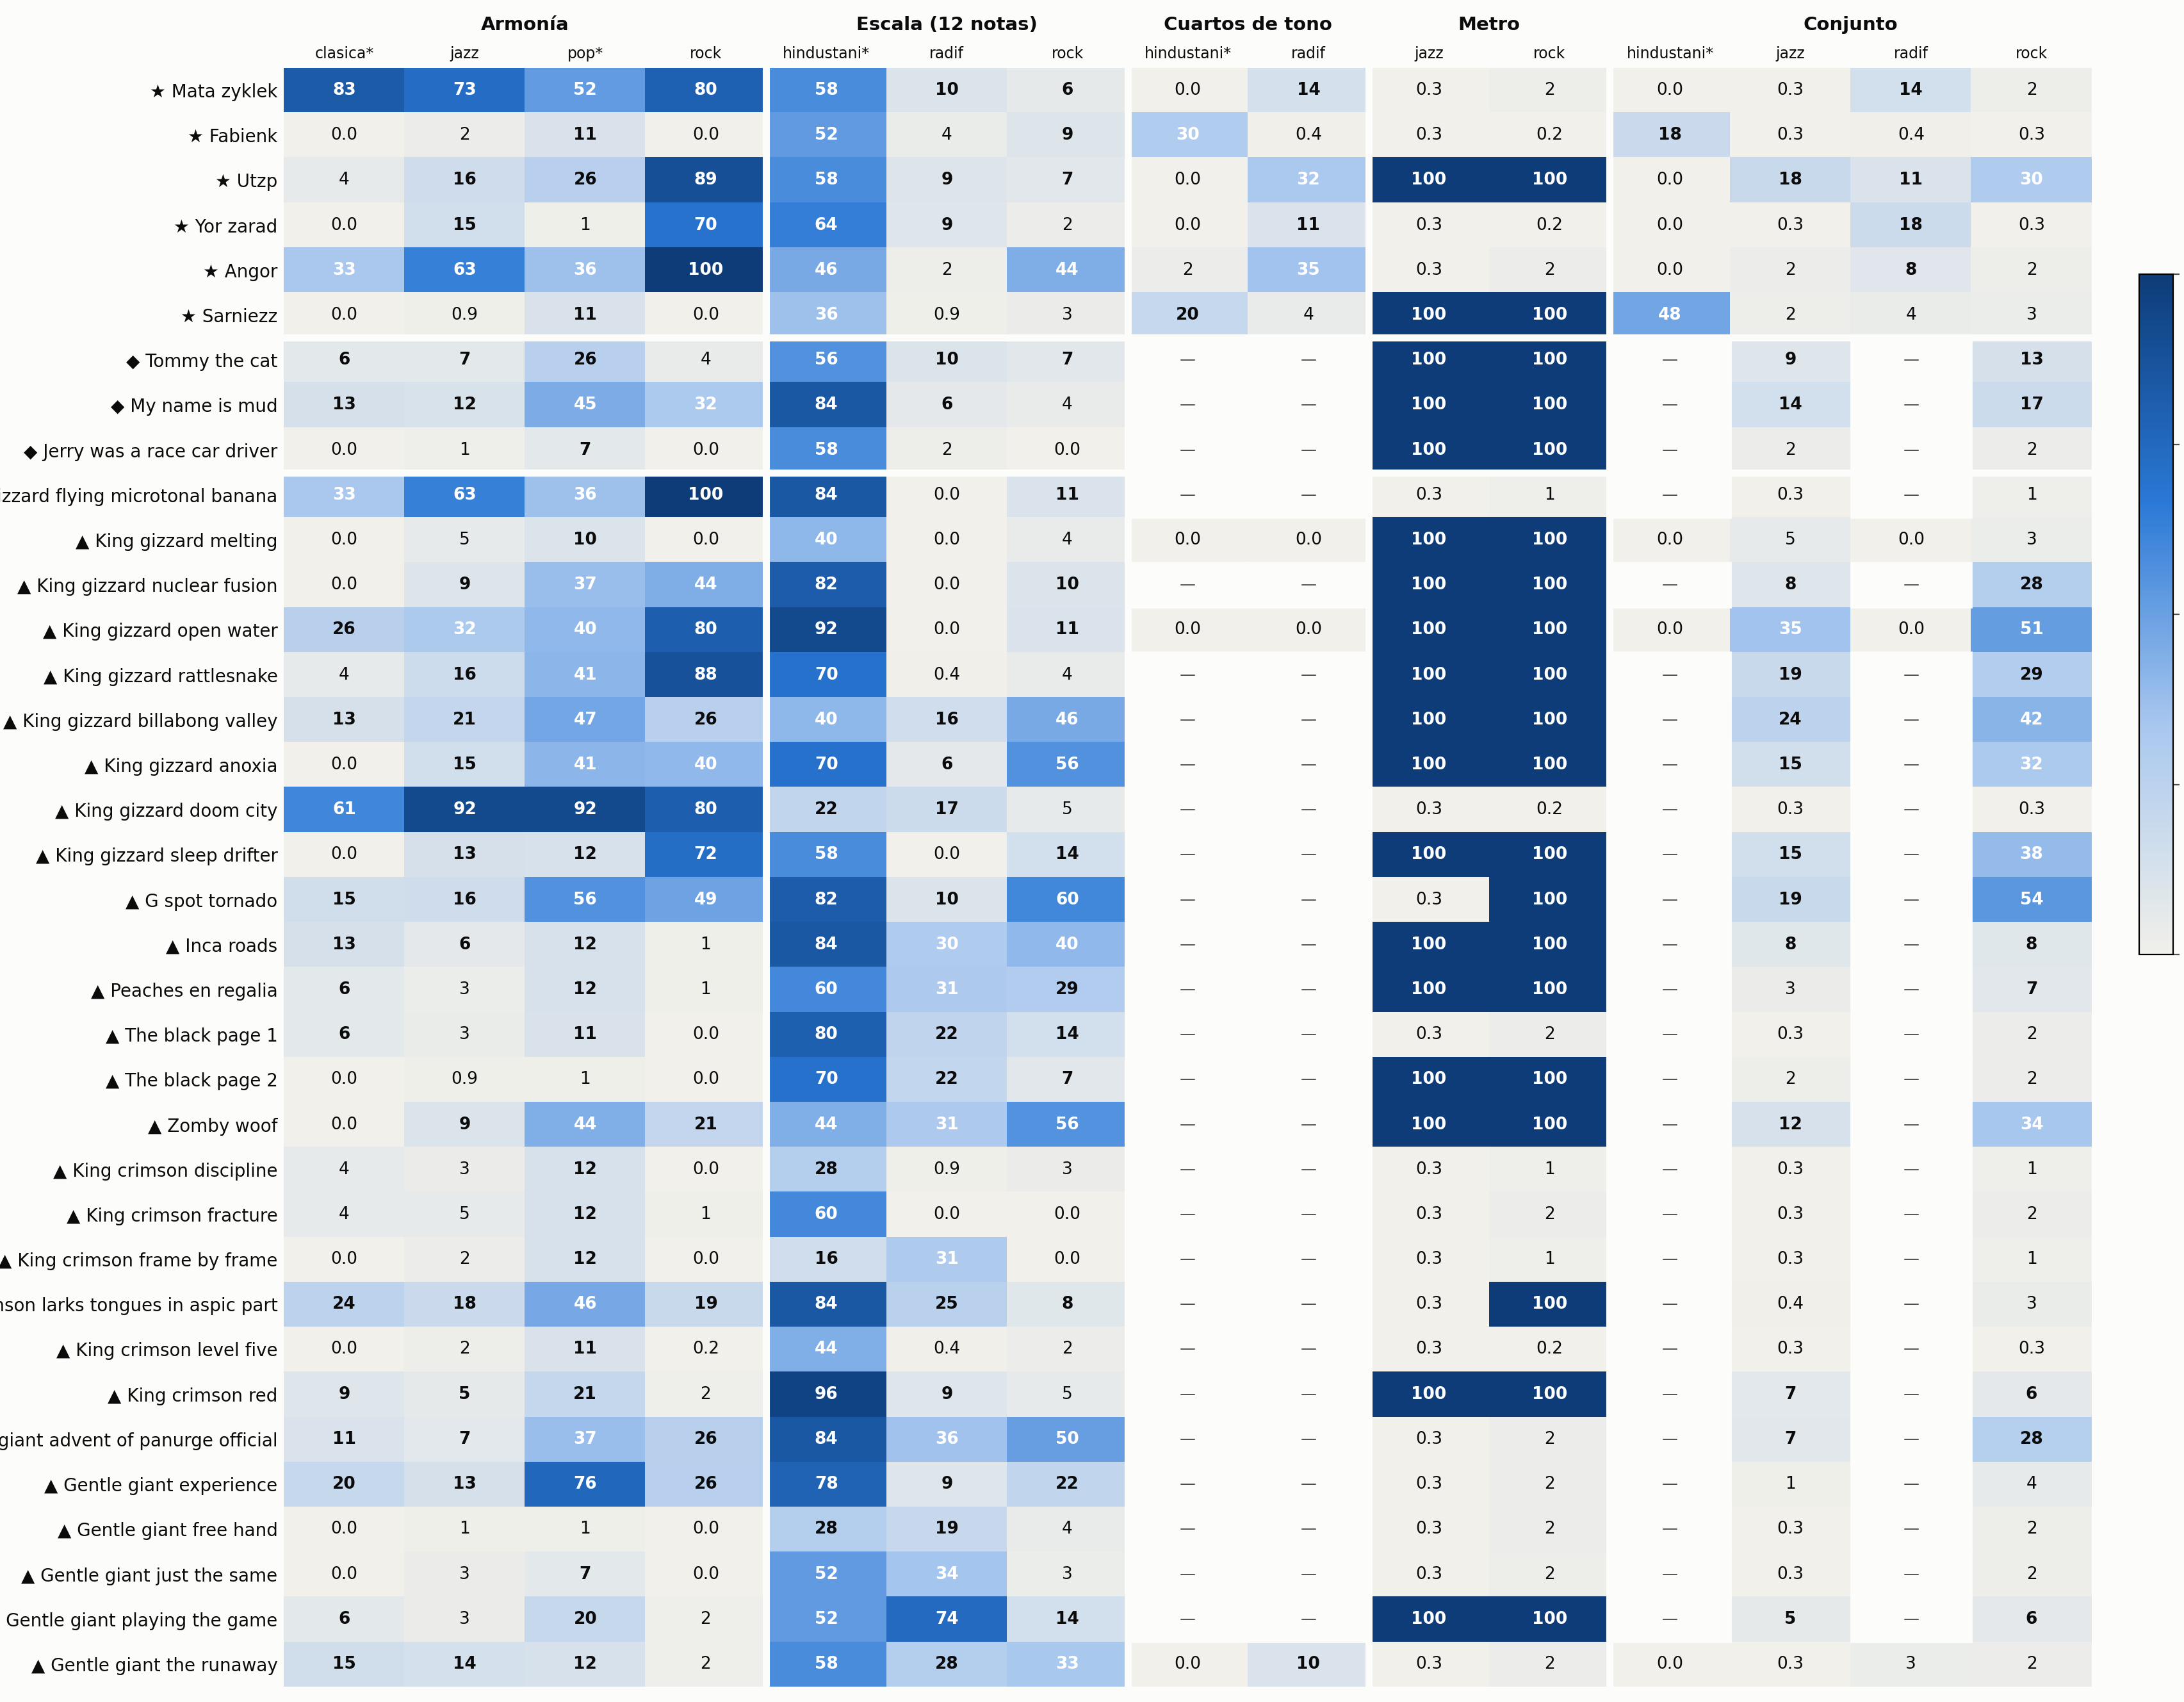
\includegraphics[width=\textwidth,height=0.78\textheight,keepaspectratio]{g_bloques.png}
  \caption{Test por bloques de las 36 canciones: percentil de cada canción en cada corpus y bloque (oscuro = típico). Símbolos: círculo, la banda; rombo, Primus; triángulo, repertorio comparado. Columnas agrupadas por bloque (armonía, escala en 12 notas, cuartos de tono, metro y conjunto). Asterisco: corpus de menos de 100 piezas (los tamaños están en la tabla~\ref{tab:corpus}); raya: sin datos. Las piezas de corpus pasan por el error de la herramienta ($\varepsilon = 0.11$ en altura, $\eta = 0.07$ en metro).}\label{fig:g-bloques}
\end{figure}

\begin{figure}[!htbp]
  \centering
  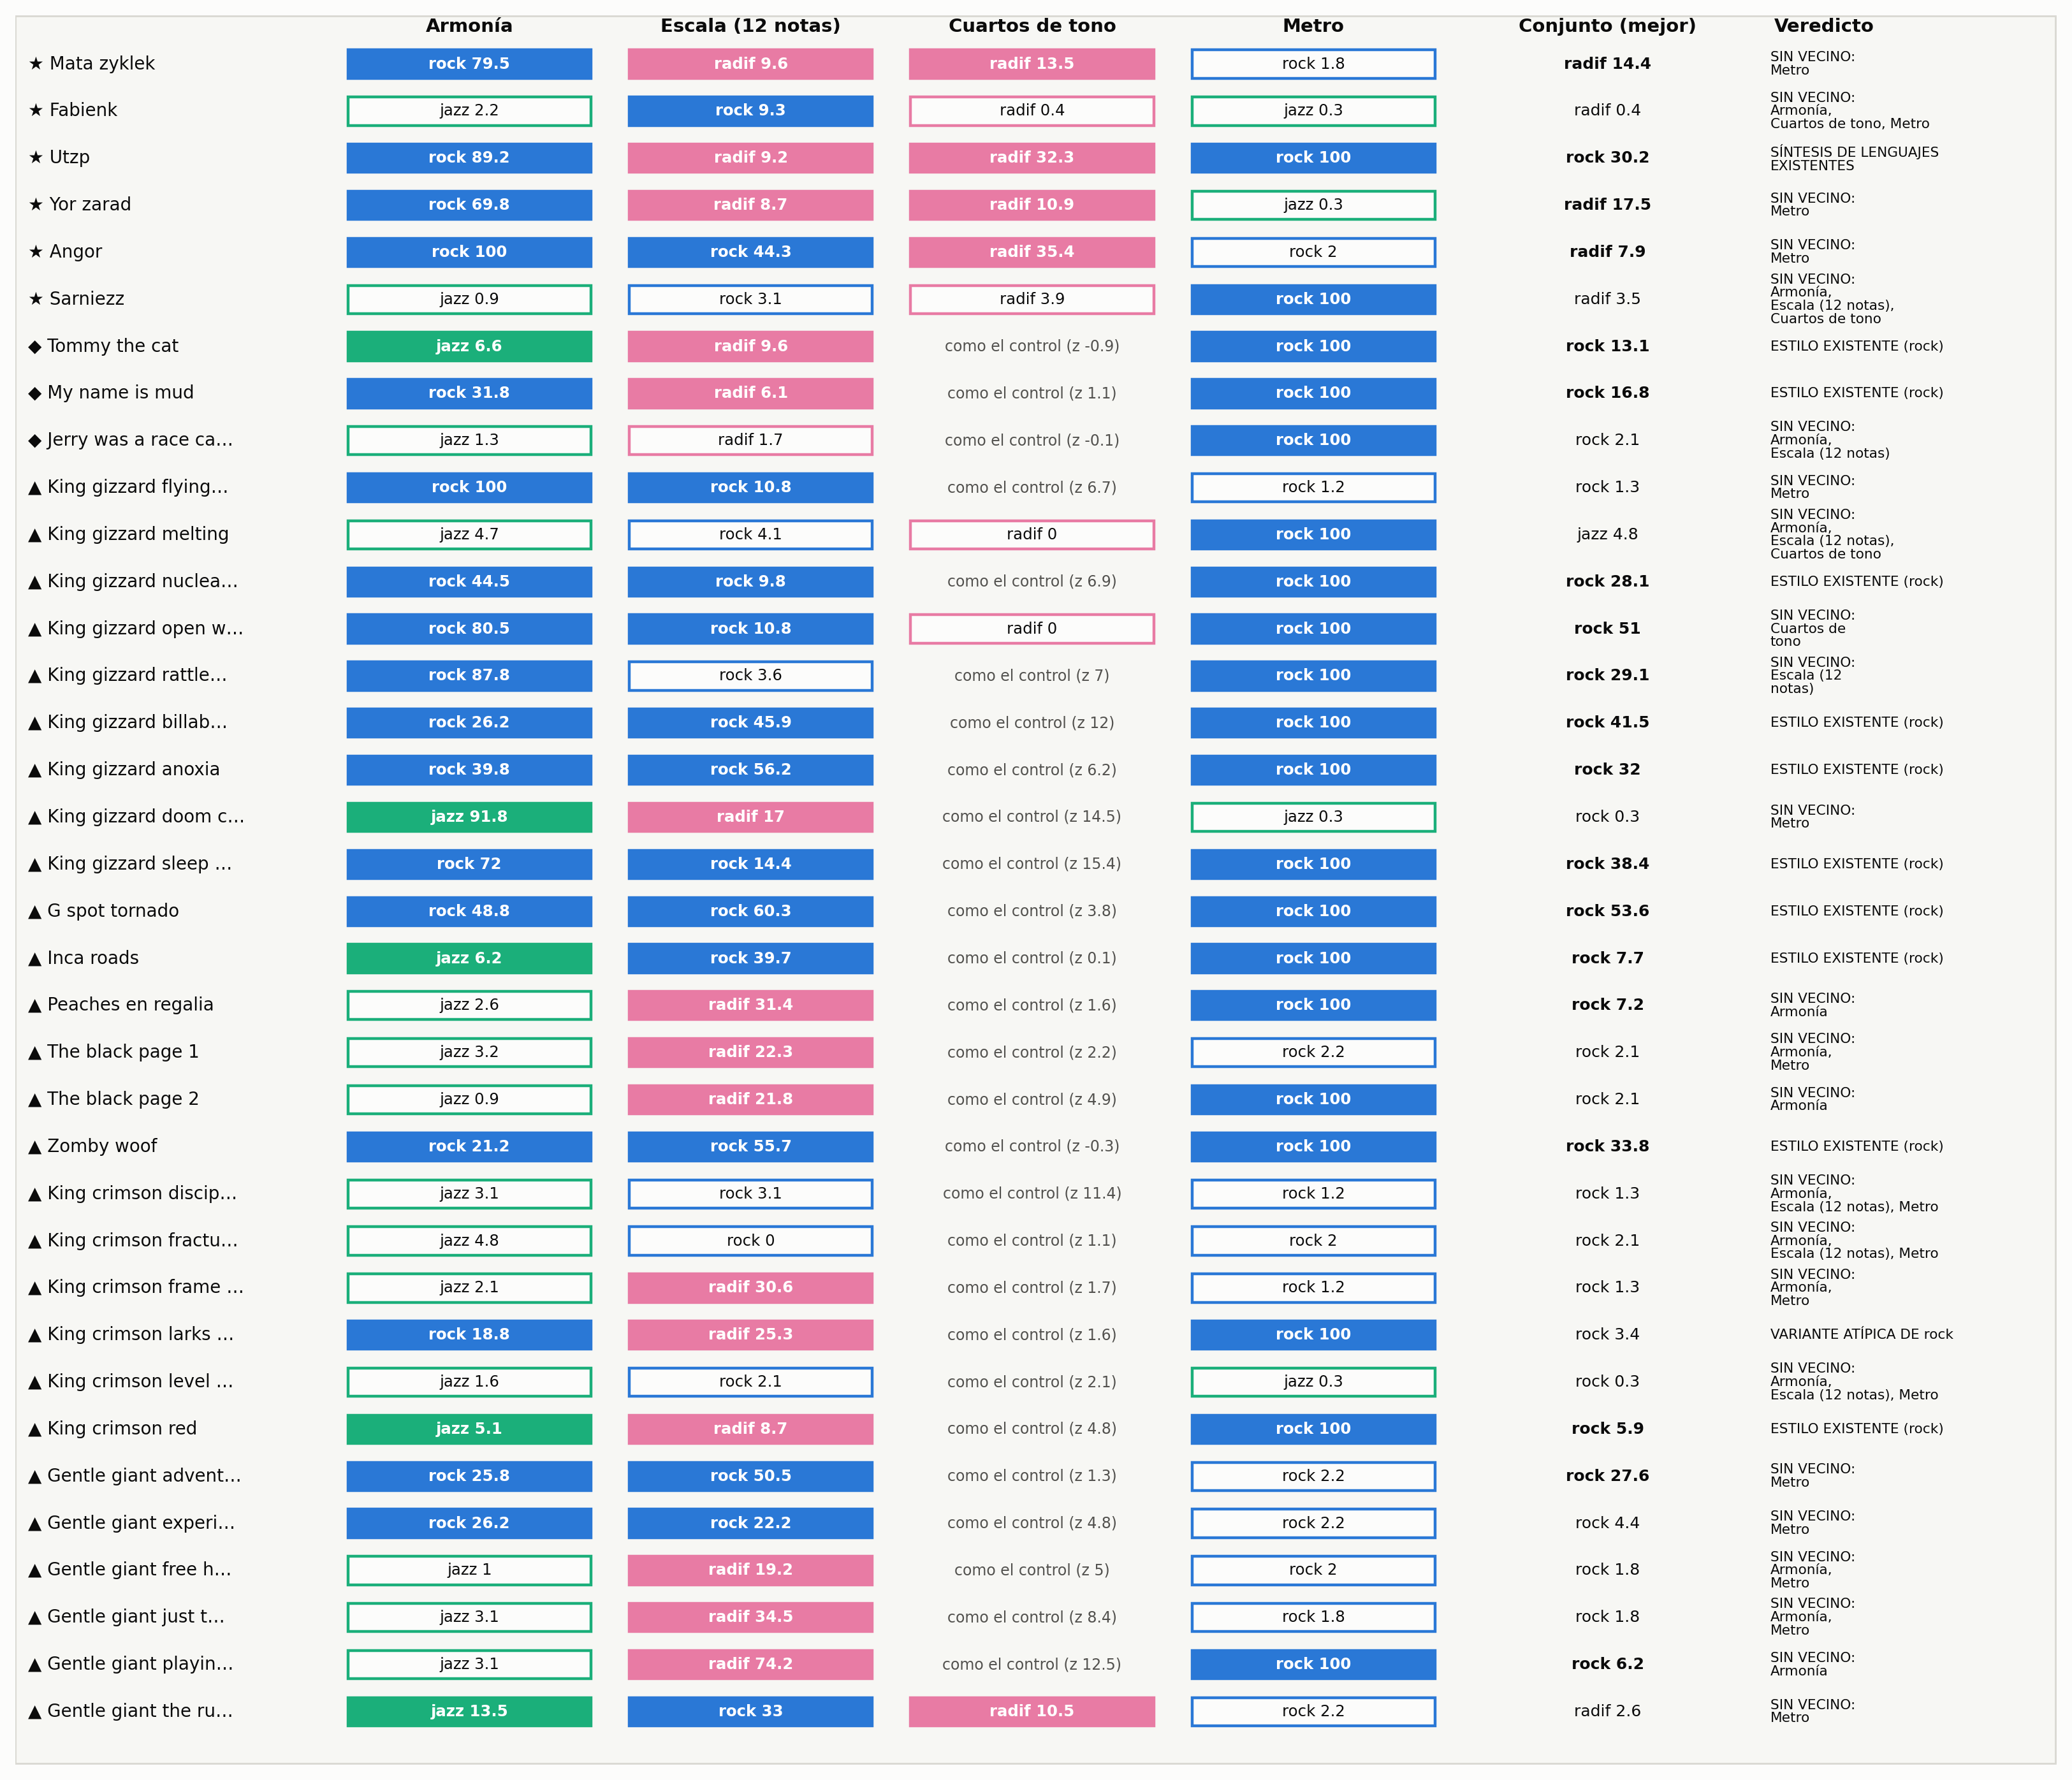
\includegraphics[width=\textwidth]{g_bloques_sintesis.png}
  \caption{Corpus más probable por bloque y veredicto de cada canción. Color: naranja, clásica; verde, jazz; rosa, microtonal; azul, rock o pop. Casilla vacía: hay datos, pero el percentil queda bajo el umbral; raya: sin datos comparables; «como el control»: concentración que no supera la de Primus. En cuartos de tono, la concentración de la banda se compara con la de Primus ($32 \pm 4$\,\%); si no la supera, no se lee como escala microtonal.}\label{fig:g-bloques-sintesis}
\end{figure}

\section{Métricas estructurales}

Las figuras~\ref{fig:tarjetas1} y~\ref{fig:tarjetas2} comparan las métricas crudas de las tarjetas para las 36
canciones (sección~\ref{sec:repertorios}).

\begin{figure}[!htbp]
  \centering
  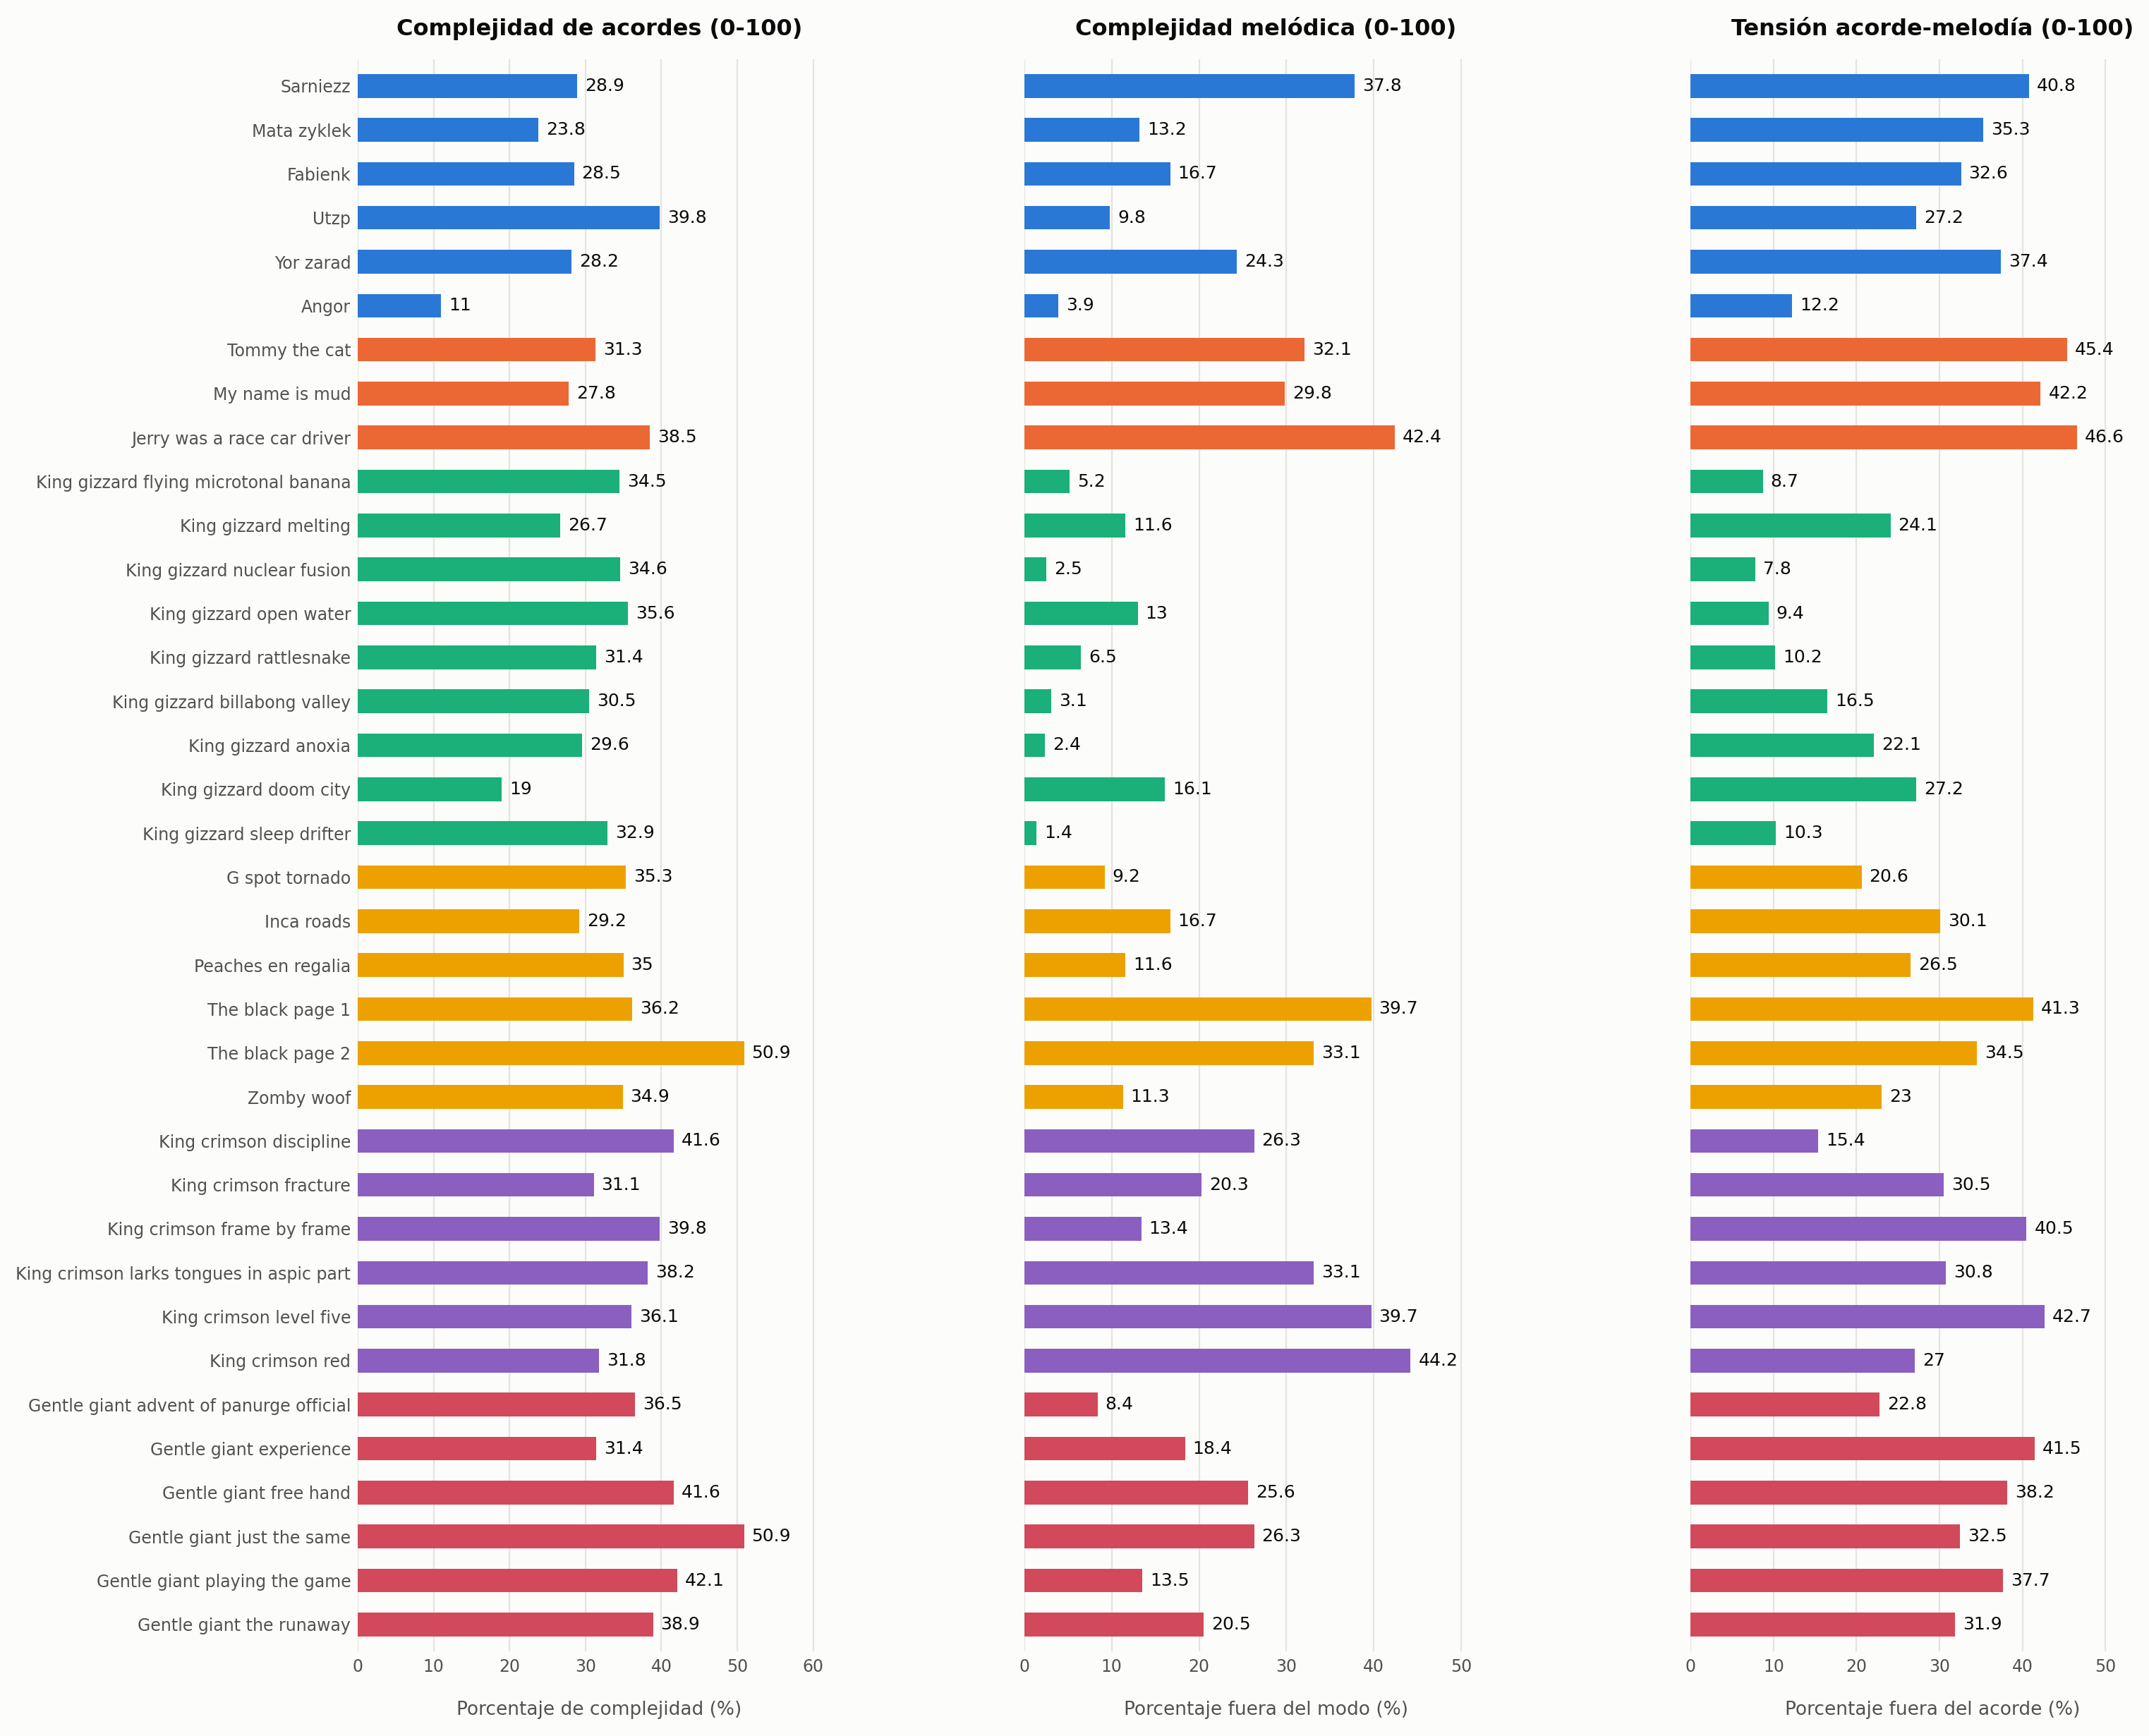
\includegraphics[width=\textwidth,height=0.78\textheight,keepaspectratio]{g_tarjetas_1.png}
  \caption{Métricas crudas de las 36 canciones (I): complejidad de acordes, complejidad melódica y tensión acorde-melodía (0--100). Color por artista: azul, la banda; naranja, Primus; verde, King Gizzard; amarillo, Zappa; violeta, King Crimson; rojo, Gentle Giant.}\label{fig:tarjetas1}
\end{figure}

\begin{figure}[!htbp]
  \centering
  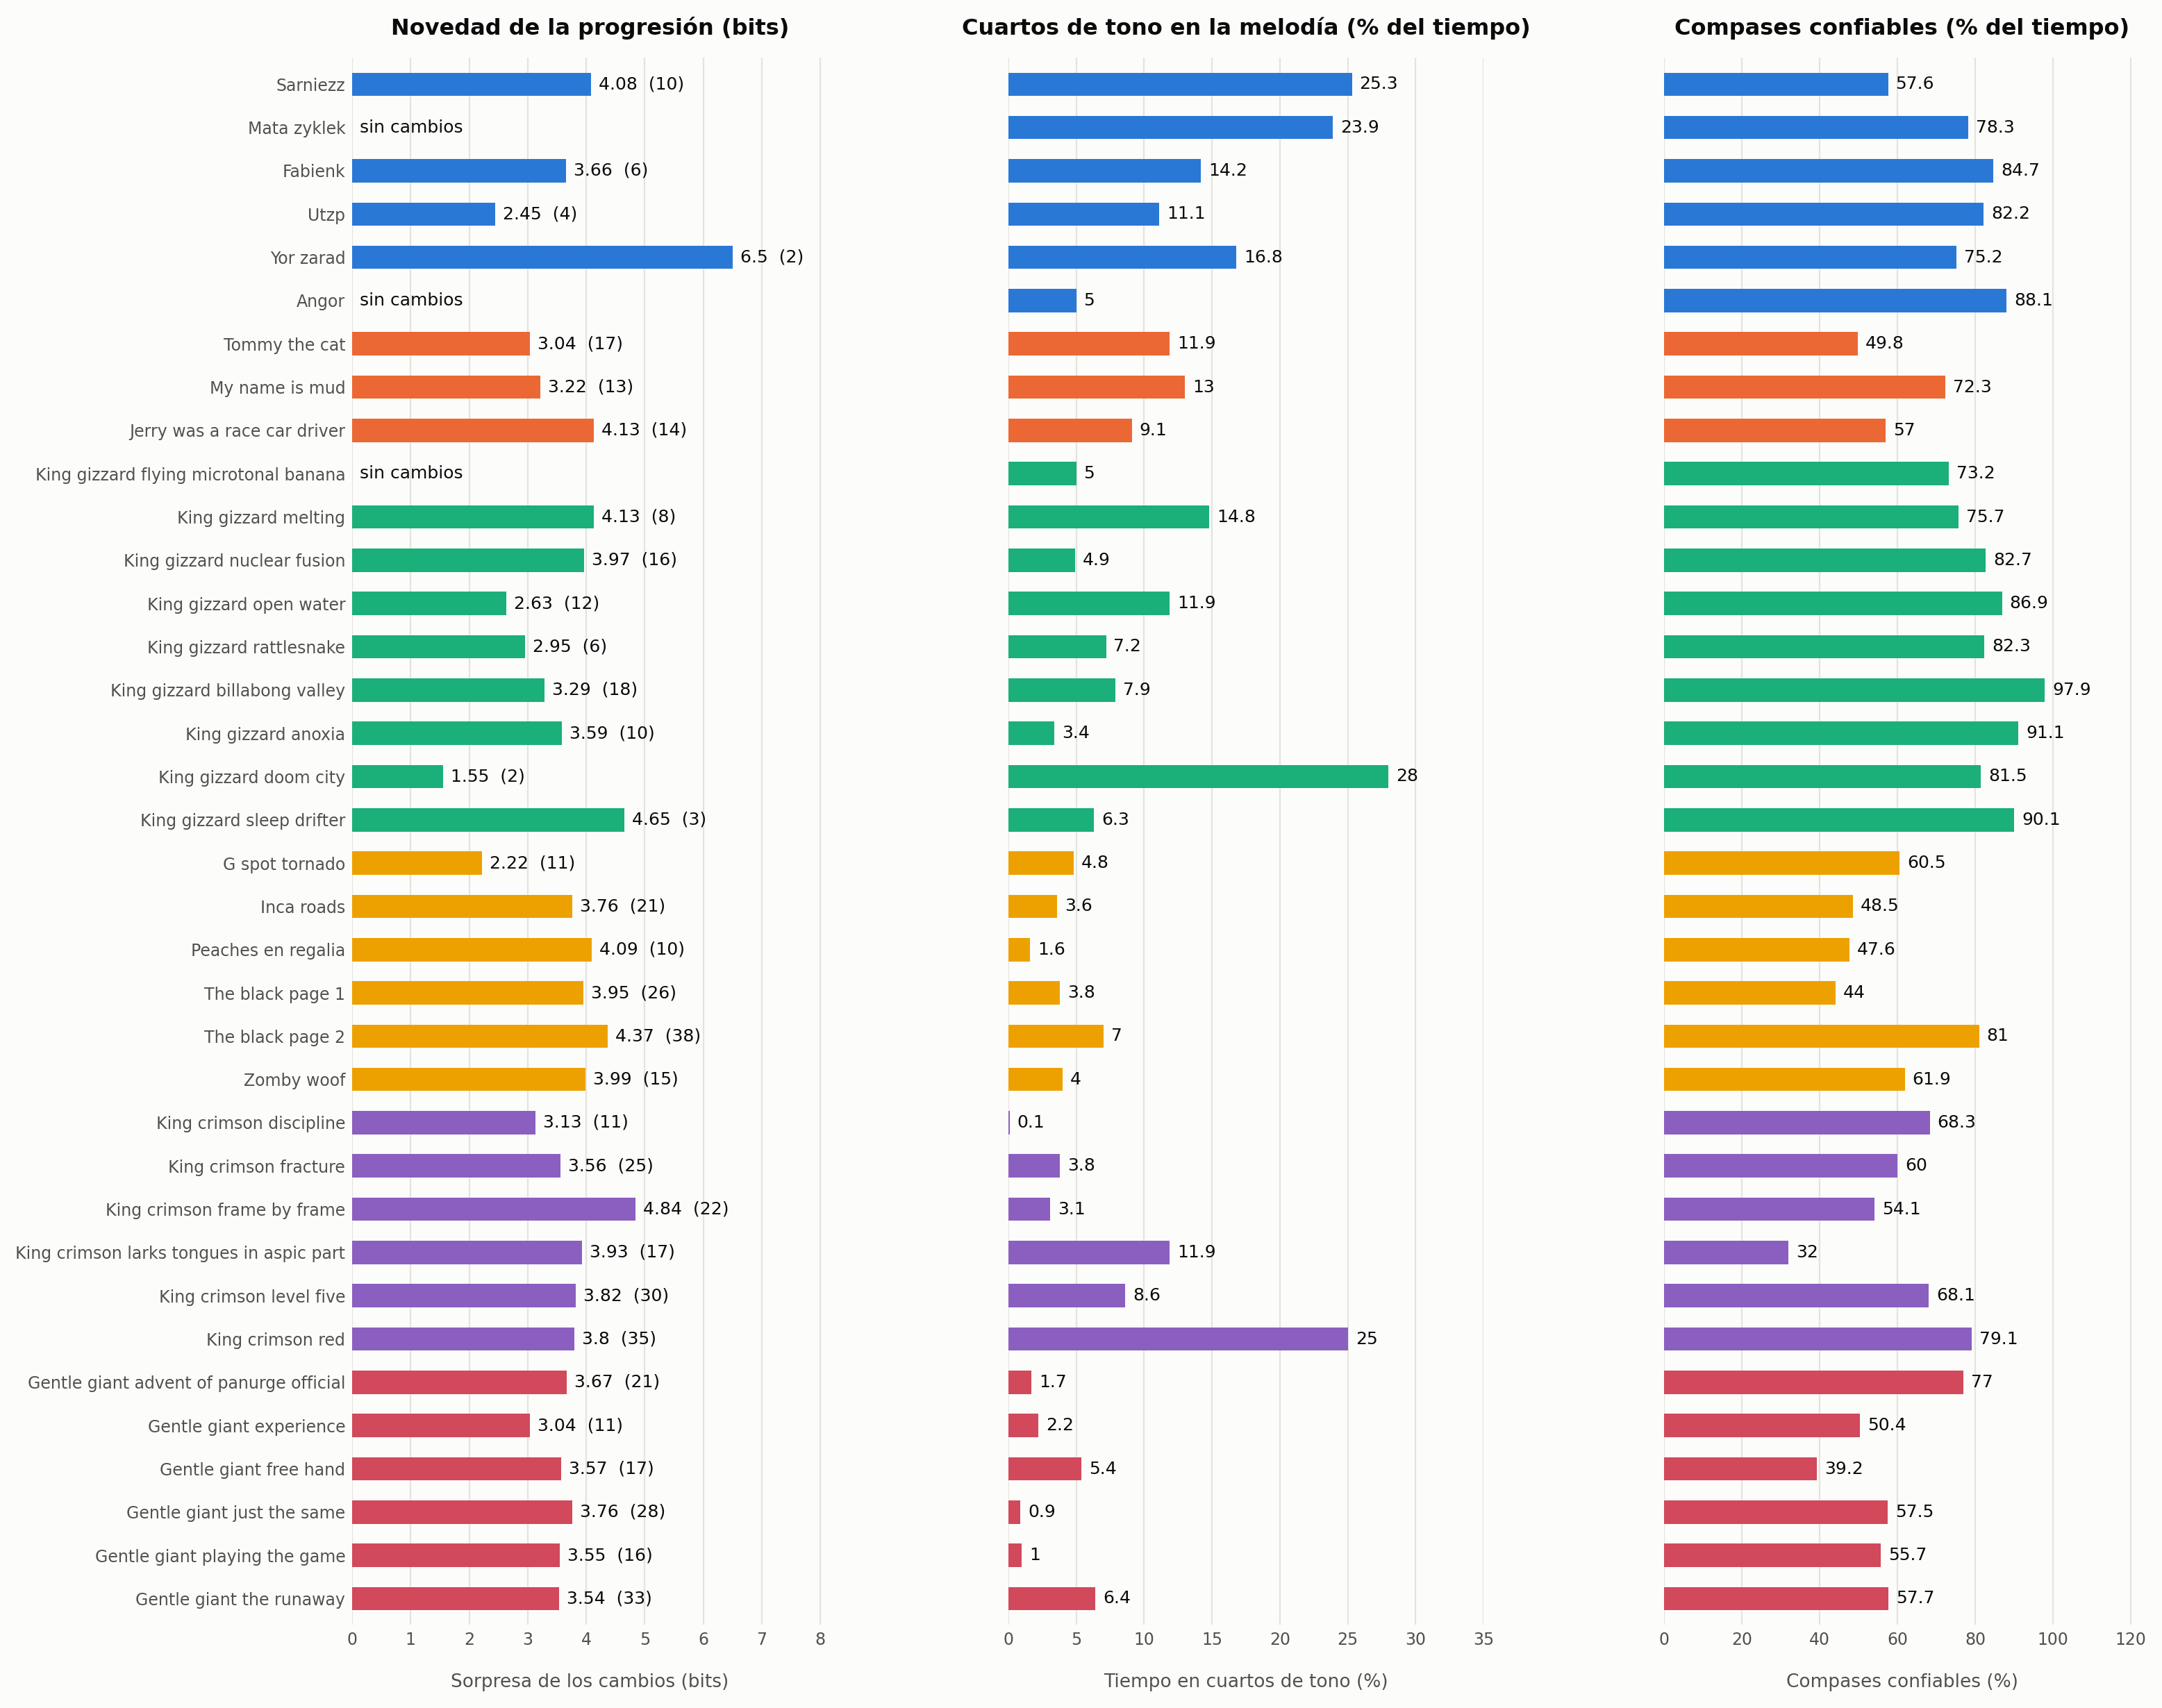
\includegraphics[width=\textwidth,height=0.78\textheight,keepaspectratio]{g_tarjetas_2.png}
  \caption{Métricas crudas (II): novedad de la progresión en bits (entre paréntesis, cambios distintos; con menos de 5 es poco estable), cuartos de tono en la melodía y compases confiables (\% del tiempo). Mismos colores que la figura~\ref{fig:tarjetas1}.}
  \label{fig:tarjetas2}
\end{figure}

\section{Radares de estilo (primera versión)}

Los radares de la figura~\ref{fig:radar-mata} (Mata Zyklek, en el capítulo~\ref{cap:metodologia}) y de las
figuras~\ref{fig:radar-fab-sar} y~\ref{fig:radar-yor-utzp} son de la versión del 15 de noviembre de 2026, anterior
al test por bloques; Angor no tenía todavía corrida en esa versión. Se incluyen como registro del método, no como
resultado.

\begin{figure}[!htbp]
  \centering
  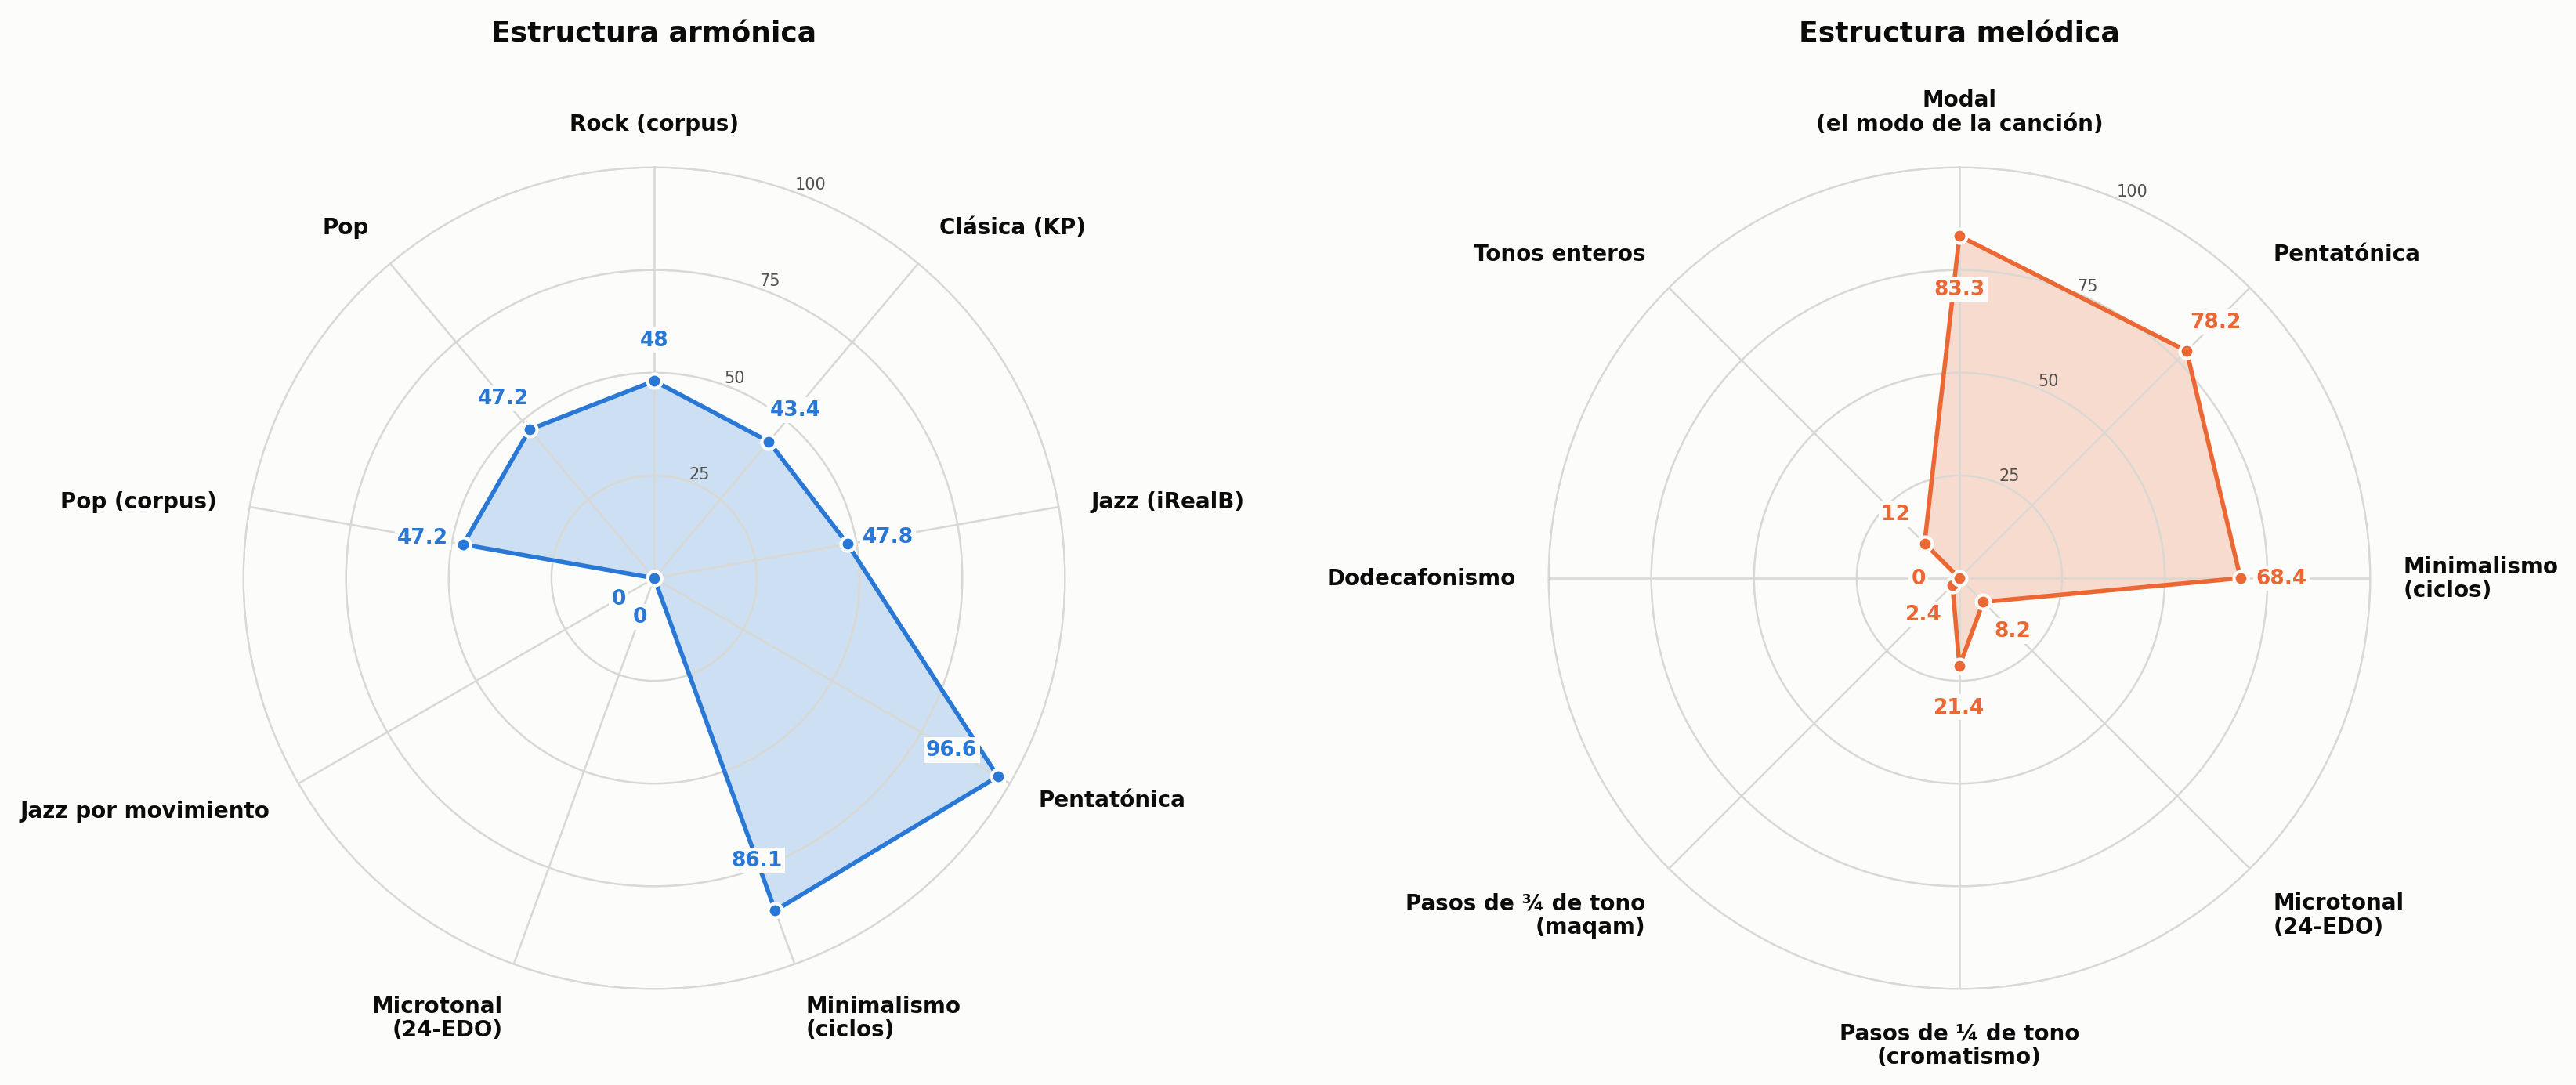
\includegraphics[width=\textwidth]{fabienk_radar_estilos.png}\\[0.5em]
  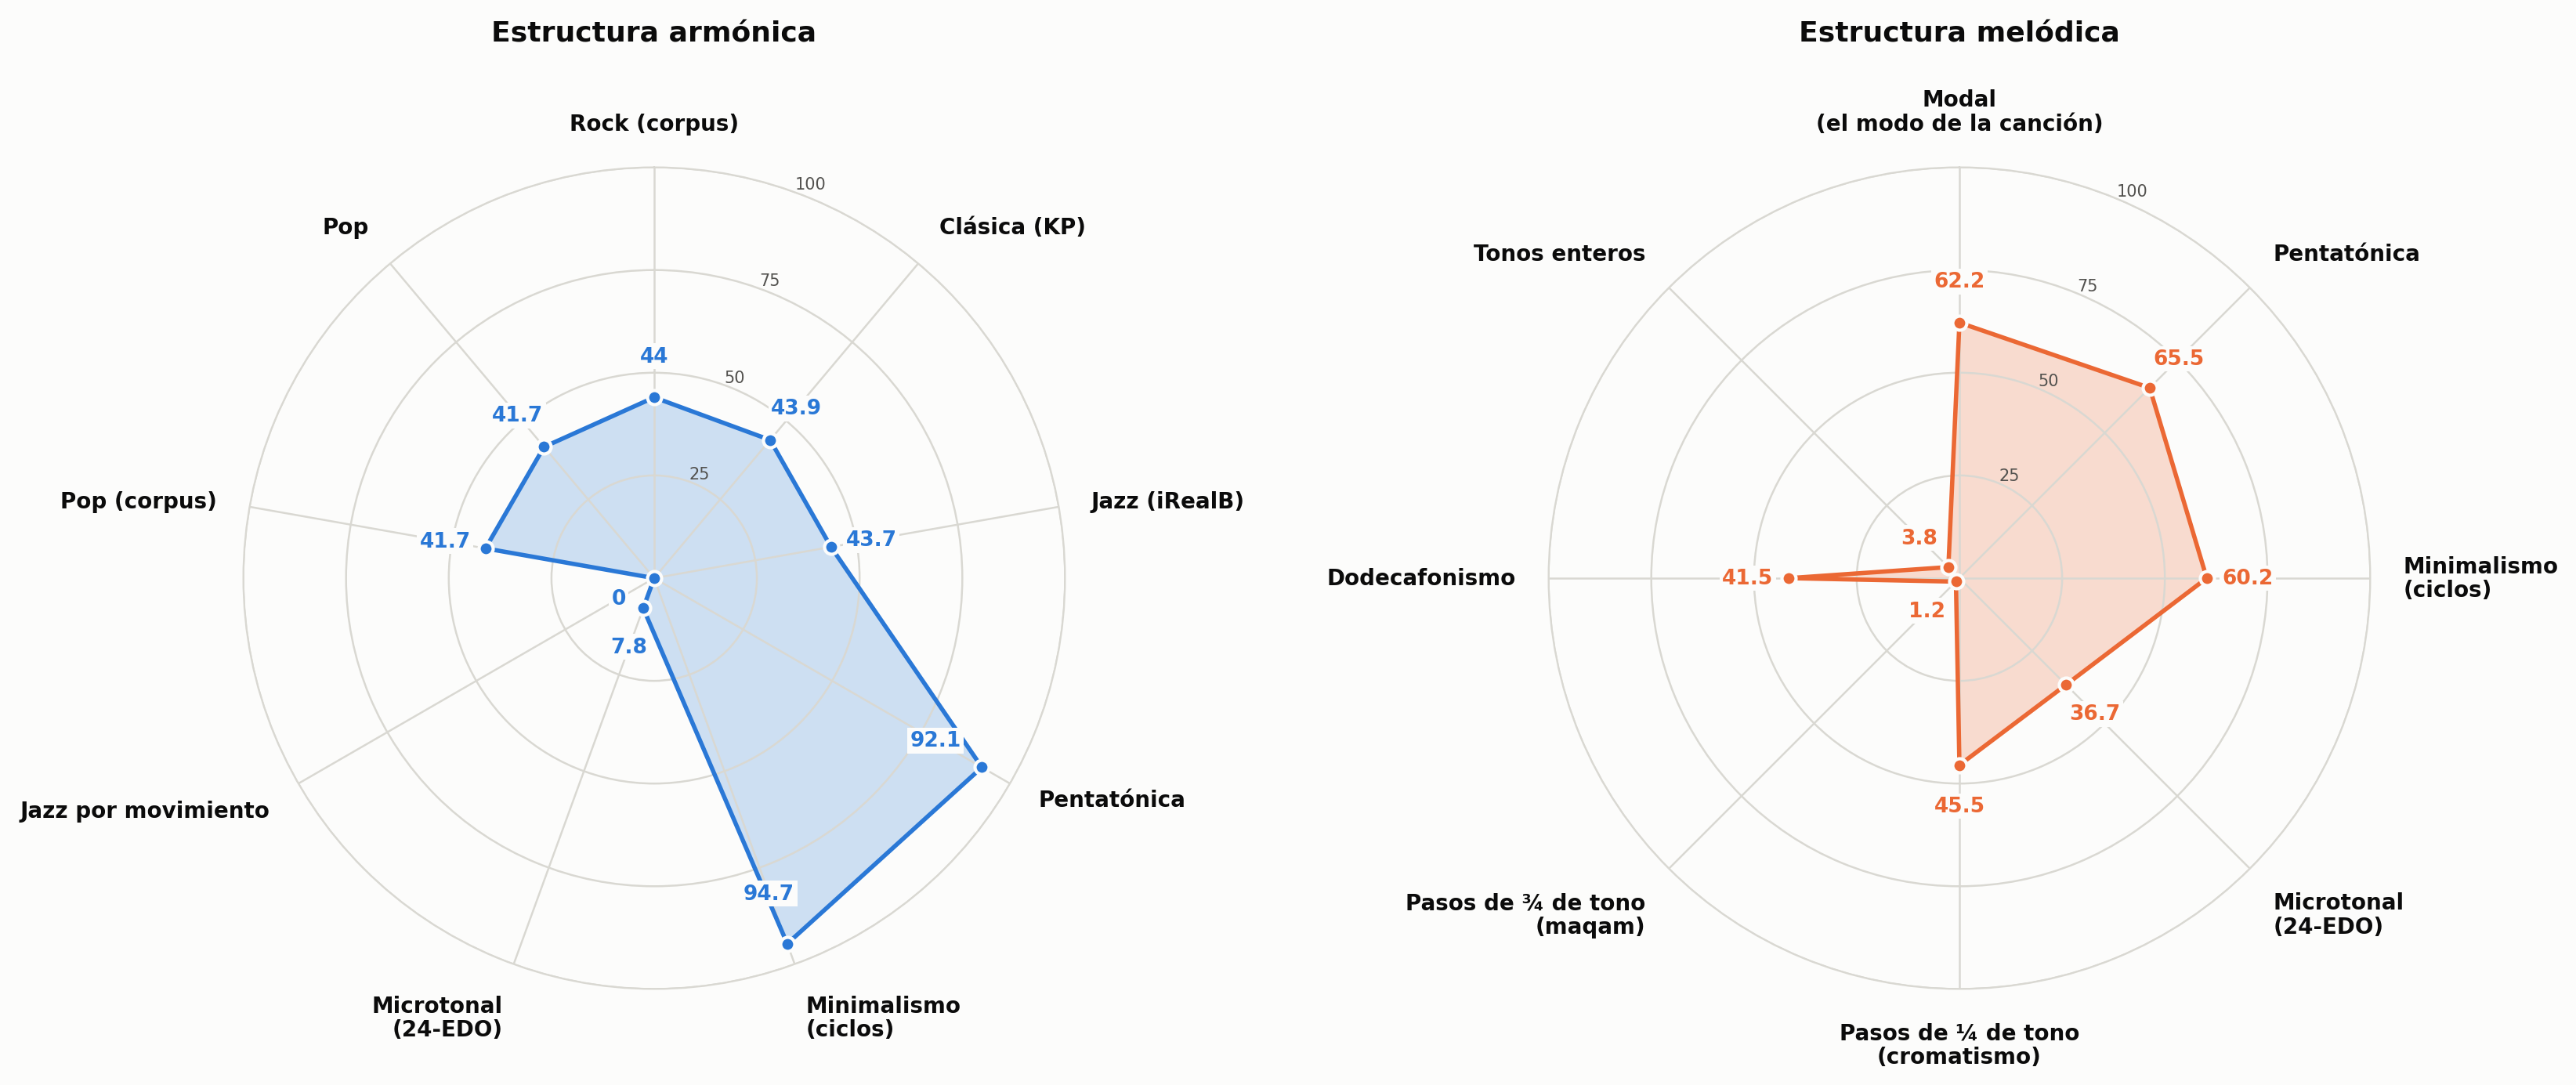
\includegraphics[width=\textwidth]{sarniezz_radar_estilos.png}
  \caption{Radares de estilo (versión descartada): Fabienk (arriba) y Sarniezz (abajo). Misma lectura que la figura~\ref{fig:radar-mata}.}\label{fig:radar-fab-sar}
\end{figure}

\begin{figure}[!htbp]
  \centering
  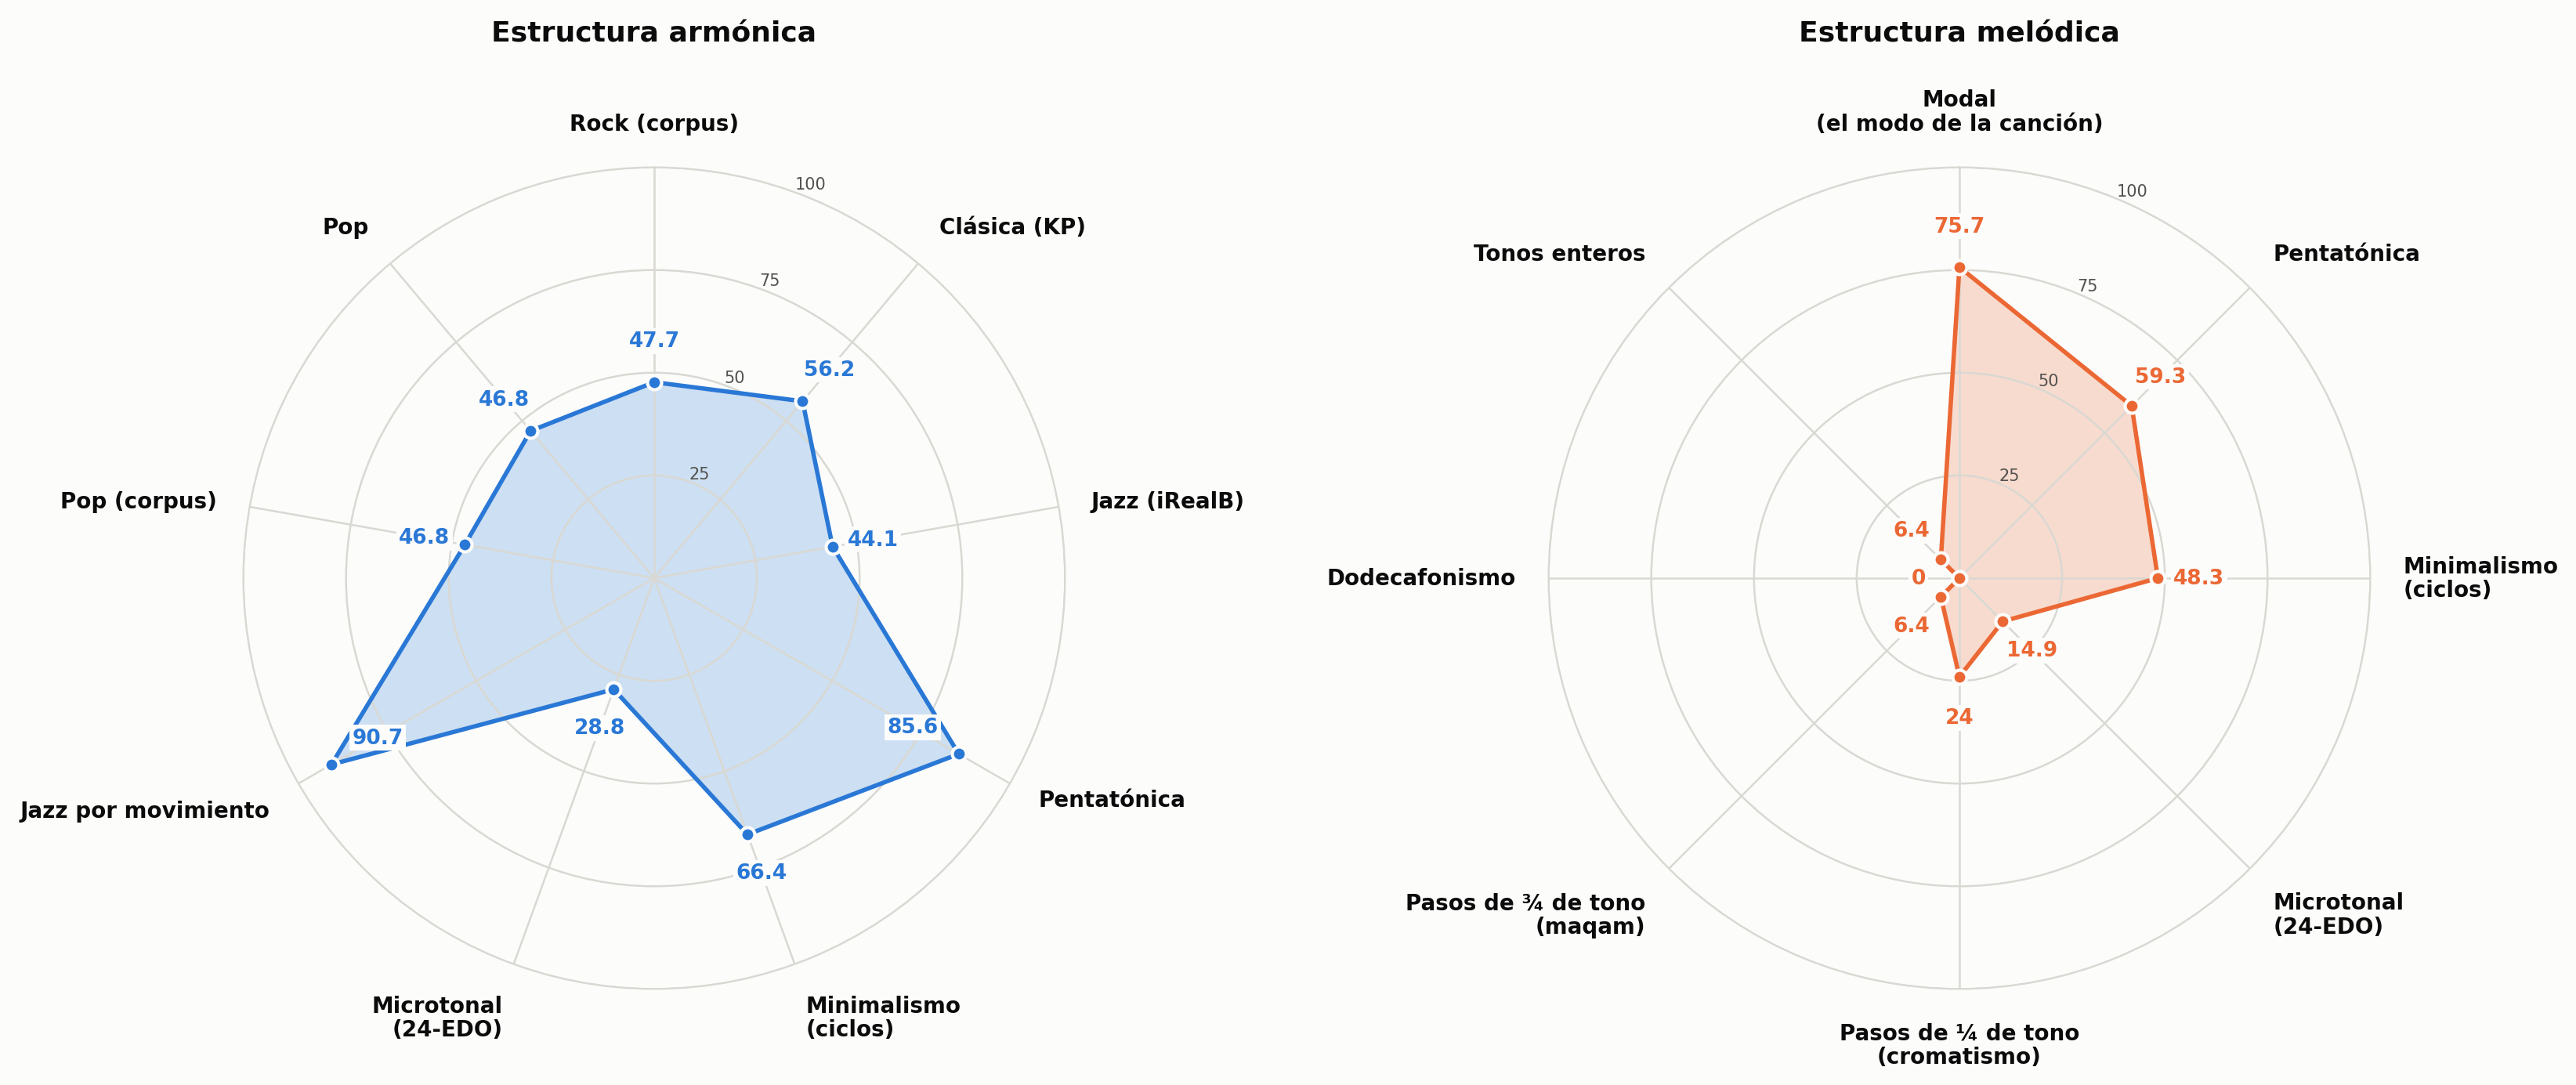
\includegraphics[width=\textwidth]{yor_zarad_radar_estilos.png}\\[0.5em]
  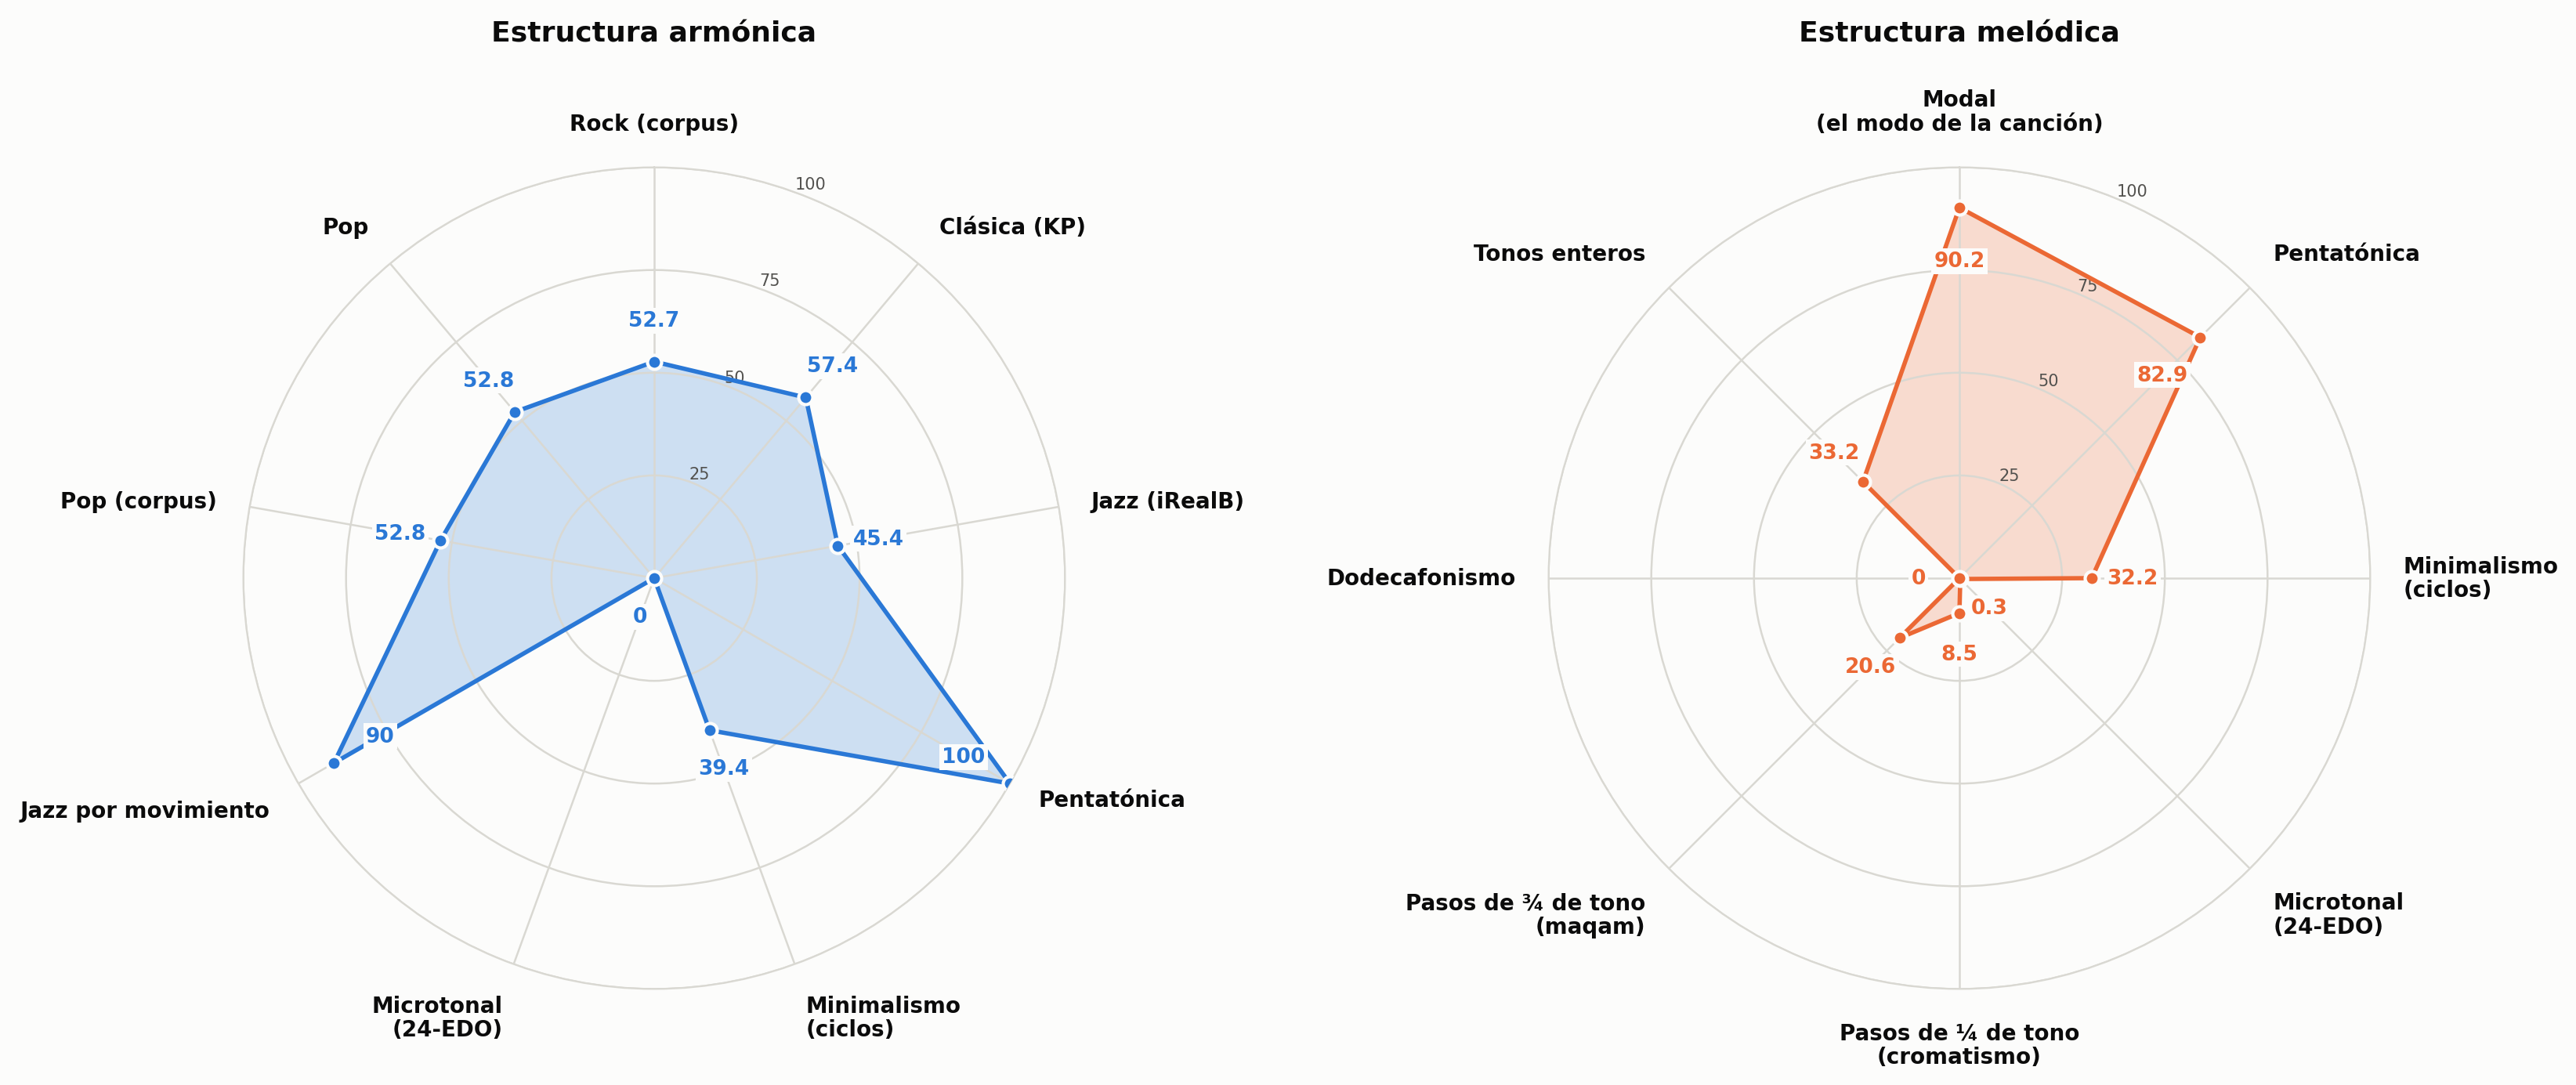
\includegraphics[width=\textwidth]{utzp_radar_estilos.png}
  \caption{Radares de estilo (versión descartada): Yor Zarad (arriba) y Utzp (abajo). Misma lectura que la figura~\ref{fig:radar-mata}.}\label{fig:radar-yor-utzp}
\end{figure}

\chapter{Círculos armónicos por canción}\label{ap:circulos}

El cuaderno dibuja, para cada canción, un círculo armónico de 24 posiciones contadas desde la tónica. Reúne el perfil del
bajo, el de la voz aguda y el de las fundamentales, las transiciones entre fundamentales y el ritmo armónico. Son la
versión por canción, en disposición cromática, de la figura~\ref{fig:circulo}.

\begin{figure}[ht]
  \centering
  \begin{subfigure}{0.48\textwidth}\centering
    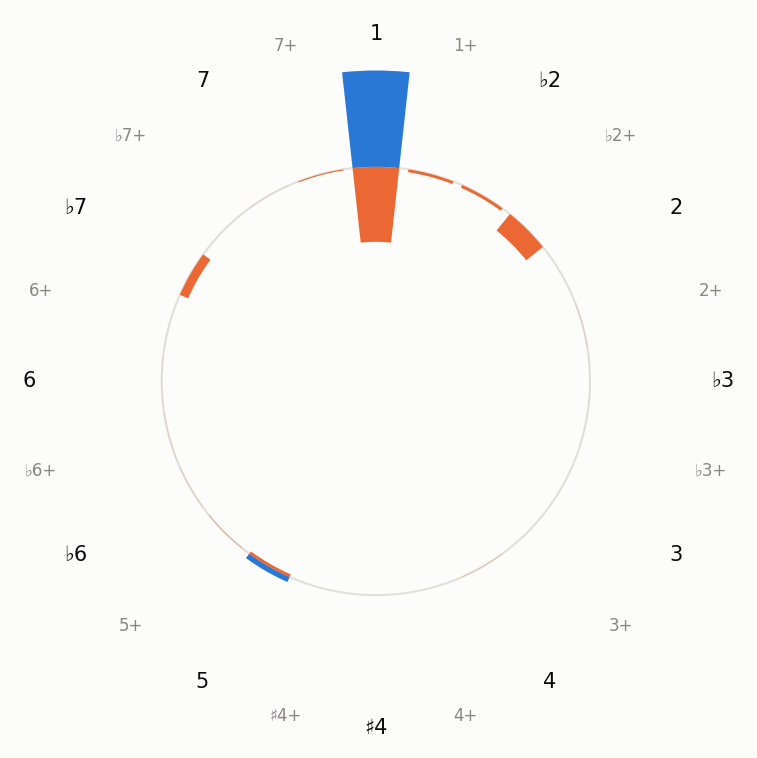
\includegraphics[width=\linewidth]{mata_zyklek_circulo_armonico.png}\caption{Mata Zyklek.}
  \end{subfigure}\hfill
  \begin{subfigure}{0.48\textwidth}\centering
    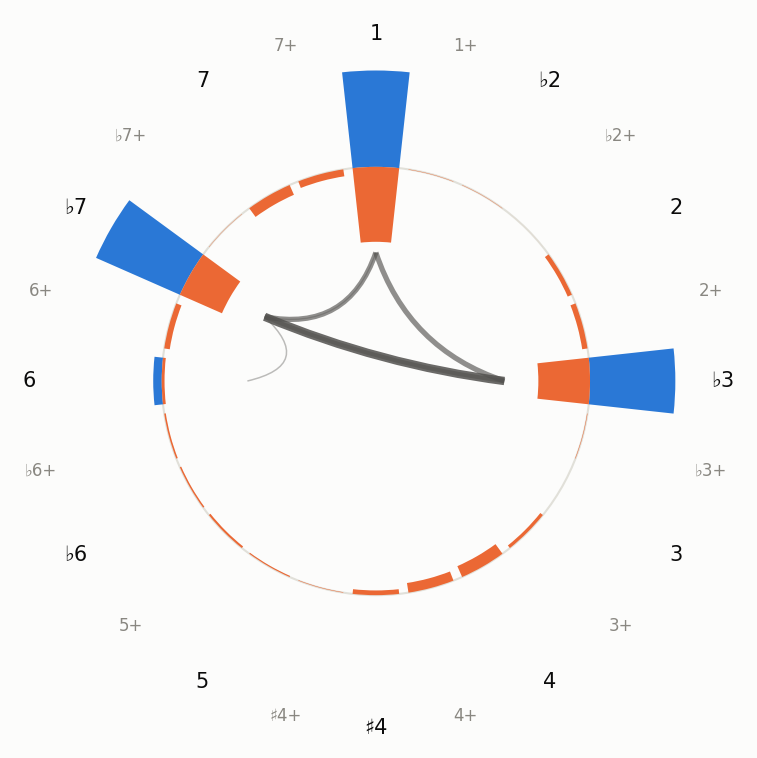
\includegraphics[width=\linewidth]{fabienk_circulo_armonico.png}\caption{Fabienk.}
  \end{subfigure}\\[0.6em]
  \begin{subfigure}{0.48\textwidth}\centering
    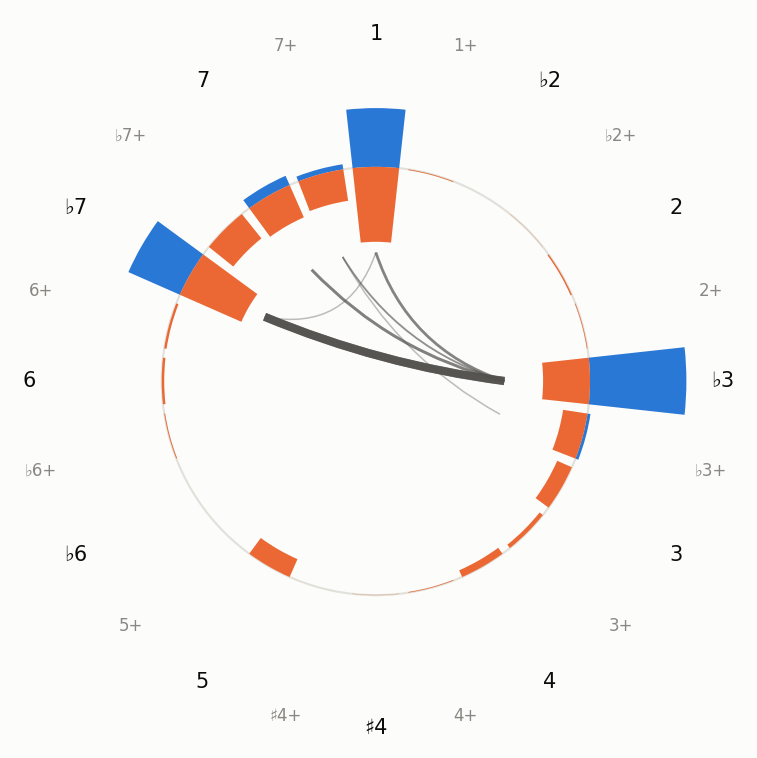
\includegraphics[width=\linewidth]{sarniezz_circulo_armonico.png}\caption{Sarniezz.}
  \end{subfigure}\hfill
  \begin{subfigure}{0.48\textwidth}\centering
    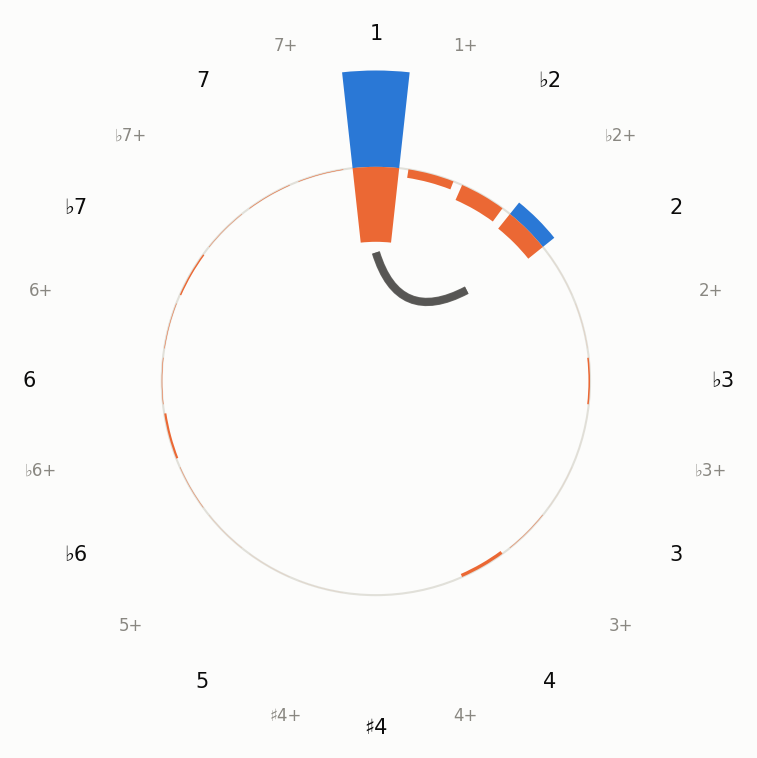
\includegraphics[width=\linewidth]{yor_zarad_circulo_armonico.png}\caption{Yor Zarad.}
  \end{subfigure}
  \caption{Círculos armónicos (I).}\label{fig:circulos1}
\end{figure}

\begin{figure}[ht]
  \centering
  \begin{subfigure}{0.48\textwidth}\centering
    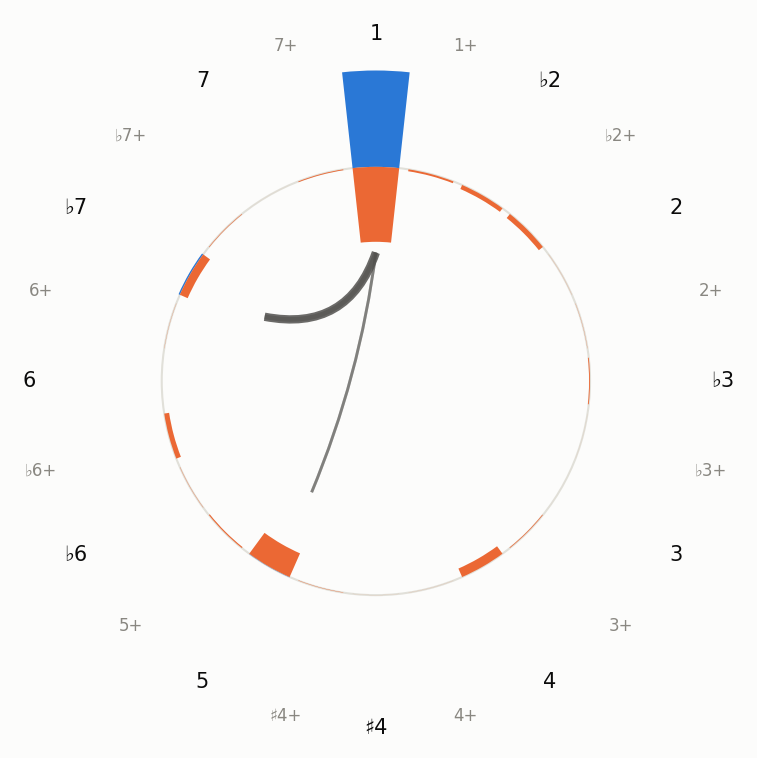
\includegraphics[width=\linewidth]{utzp_circulo_armonico.png}\caption{Utzp.}
  \end{subfigure}\hfill
  \begin{subfigure}{0.48\textwidth}\centering
    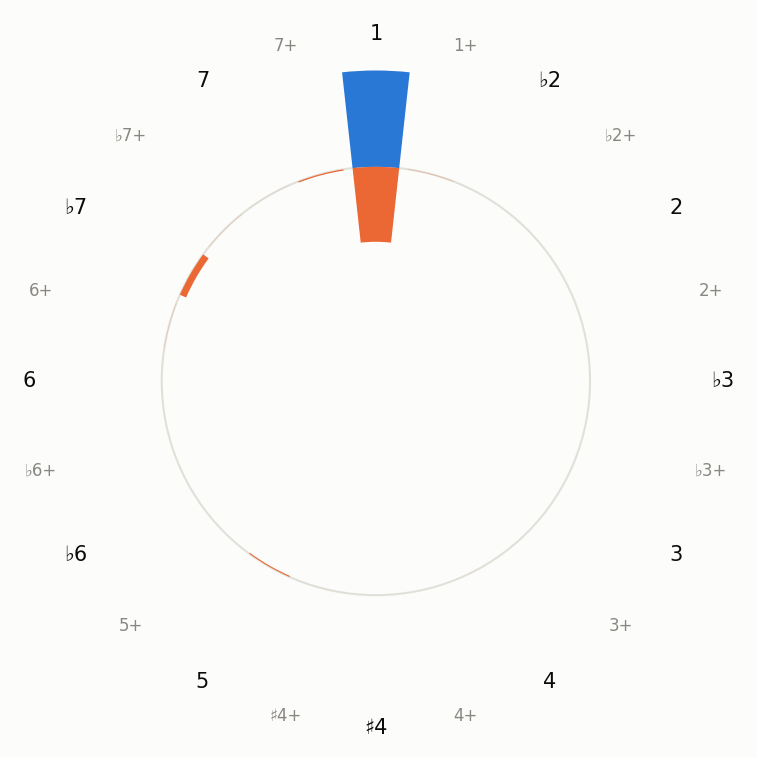
\includegraphics[width=\linewidth]{angor_circulo_armonico.png}\caption{Angor.}
  \end{subfigure}
  \caption{Círculos armónicos (II).}\label{fig:circulos2}
\end{figure}

\chapter{Glosario}\label{ap:glosario}

\section*{Altura y afinación}
\begin{description}[style=nextline,leftmargin=1.2em]
  \item[Cent] Centésima parte de un semitono temperado; la octava mide 1200 cents.
  \item[$q$-EDO] Sistema que divide la octava en $q$ partes iguales. 12-EDO es el temperamento usual; 24-EDO divide cada
  semitono en dos cuartos de tono de 50 cents.
  \item[Cuarto de tono] Intervalo de 50 cents. En este trabajo se escribe «+» sobre la nota o el grado (Sol+, \fl2+).
  \item[Clase de altura] Altura sin importar la octava; en 24-EDO hay 24 clases.
  \item[MIDI fraccionario] Número de nota continuo: $69 + 12\log_2(f/440)$. 52.5 es un cuarto de tono sobre Mi.
  \item[Campo] Cada una de las dos órbitas del ciclo de quintas en 24-EDO: grados regulares y grados en cuarto de tono.
  \item[Tercera neutra] Tercera de 350 cents, entre la menor y la mayor; solo existe con cuartos de tono.
  \item[Grado fijo] Nota de la escala que vuelve en cada vuelta del loop, a diferencia de un adorno de paso.
  \item[Inflexión] Cuarto de tono breve que llega o sale por un paso de cuarto de tono hacia un grado regular: un bend, un
  slide o una nota de paso.
  \item[Piso de ruido] Tiempo en cuartos de tono que la herramienta marca en música sin cuartos de tono (Primus, 9--13\,\%).
\end{description}

\section*{Señal y transcripción}
\begin{description}[style=nextline,leftmargin=1.2em]
  \item[Espectrograma] Energía de cada frecuencia en cada instante, calculada con la transformada de Fourier de tiempo
  corto.
  \item[Saliencia armónica] Evidencia de cada altura candidata, obtenida sumando la energía de sus armónicos.
  \item[pYIN] Estimador de la frecuencia fundamental de una sola voz \citep{mauch2014}.
  \item[Viterbi] Algoritmo de programación dinámica que elige la sucesión de estados de mayor puntaje.
  \item[MFCC] Coeficientes cepstrales en escala Mel: describen el timbre, no la nota.
  \item[Separación de fuentes] Extracción de la pista de cada instrumento a partir de la mezcla (Demucs, BS-RoFormer).
  \item[SDR] \emph{Signal-to-distortion ratio}: qué tan limpia sale una pista separada, en decibeles.
  \item[Looper] Dispositivo que graba una frase y la repite en bucle mientras se toca encima.
  \item[Ciclo] Tramo en que una voz repite un patrón con un periodo fijo; cada ciclo distinto recibe una letra.
  \item[Consenso entre vueltas] Promedio de la saliencia en los instantes equivalentes de vueltas vecinas del ciclo.
  \item[Piano roll] Gráfica con el tiempo en el eje horizontal y la altura en el vertical.
  \item[Tabroll] El piano roll de este trabajo: 24 filas por octava, compases y un acorde por compás, generado desde el
  audio.
\end{description}

\section*{Armonía}
\begin{description}[style=nextline,leftmargin=1.2em]
  \item[Fundamental] Nota que da nombre al acorde.
  \item[Calidad] Tipo de acorde según sus intervalos: quinta sola, menor, neutro, mayor, disminuido, aumentado, sus2 o
  sus4.
  \item[Centro] La nota de reposo de la canción; aquí se mide en tres partes (tiempo, bordes de vuelta y regresos).
  \item[Grado y cifrado] Posición de la fundamental respecto del centro, escrita en números romanos (I, \fl III, \fl VII,
  \fl II+).
  \item[Función] Papel del acorde según Riemann: tónica, subdominante o dominante; neutra para los grados en cuarto de tono.
  \item[Eje] Grupo de grados a distancia de tercera menor que comparten función, según Lendvai.
  \item[Pedal] Nota que se sostiene o se repite mientras la armonía se mueve encima.
  \item[Vaivén] Ida y vuelta repetida entre dos acordes.
  \item[Confianza $\kappa$] Qué tan segura está la herramienta del acorde de un compás; confiable si $\kappa \ge 0.5$.
  \item[Modo] Escala de siete grados con un centro (dórico, frigio, frigio dominante\dots).
\end{description}

\section*{Comparación y evaluación}
\begin{description}[style=nextline,leftmargin=1.2em]
  \item[Corpus] Colección de piezas de un estilo guardadas como notas o acordes.
  \item[Reparto de fundamentales] Fracción del tiempo que la canción pasa sobre cada grado.
  \item[Divergencia de Jensen-Shannon] Medida de diferencia entre dos repartos, de 0 (iguales) a 1 (nada en común).
  \item[Percentil de tipicidad] Porcentaje de piezas del corpus igual o más lejos que la canción: 50 es típica, 0 más rara
  que todas.
  \item[Bloque de rasgos] Conjunto de medidas de una dimensión: armonía, escala, cuartos de tono o metro.
  \item[Sin vecino] Ningún corpus llega al percentil 5 en un bloque.
  \item[Calibración] Aplicar el método a piezas cuya respuesta se conoce para medir cuánto se equivoca.
  \item[Medida F] Media armónica de la precisión y la exhaustividad de una transcripción.
  \item[Referencia corregida de oído] Partitura verificada por el autor contra fragmentos de la grabación.
  \item[Arbitraje a ciegas] Escucha de versiones en orden al azar, sin saber cuál es de la partitura y cuál de la
  herramienta.
  \item[Semilla fija] Valor que fija el azar del programa para que cada corrida dé lo mismo.
  \item[Huella SHA-256] Código de 64 caracteres que identifica un archivo y cambia si el archivo cambia \citep{nist2015}.
\end{description}


\end{document}
